\documentclass[a4paper,openright,11pt]{book}
%\documentclass[b5paper,openright,12pt]{book}
\usepackage[utf8]{inputenc}
\usepackage{graphicx,color}
\usepackage[dvipsnames]{xcolor}
\usepackage{amsfonts}
\usepackage{amsmath}
\usepackage{amssymb}
\usepackage{verbatim}
\usepackage{cite} 
\usepackage{fancyhdr}
\usepackage{epigraph}
\usepackage{caption}
\usepackage{psfrag}
\usepackage{hyperref}
\captionsetup[figure]{font=footnotesize,labelfont=footnotesize}
\graphicspath{{./figures/}}
%To use a kind of times new roman font style
\usepackage{mathptmx}
\usepackage{newtxtext,newtxmath}
\usepackage[titletoc]{appendix}
%To modify the space before title of each chapter
%\usepackage{titlesec}
%\titleformat{\chapter}[display]   
%{\normalfont\huge\bfseries}{\chaptertitlename\ \thechapter}{20pt}{\Huge}   
%\titlespacing*{\chapter}{0pt}{-10pt}{40pt}
%Modificar encabezado y pie de página.
\pagestyle{fancy}
\fancypagestyle{chapters}{%
\fancyhead{}
\fancyhead[LE,RO]{\thepage}
\fancyhead[RE]{Nanoscale hydrodynamics near solids}
\fancyhead[LO]{{\color{Gray}CHAPTER \thechapter.} \leftmark }
\fancyfoot{}
\renewcommand{\headrulewidth}{1pt}
}
%\fancyfoot[LE,RO]{\thepage}
%\fancyfoot[LO,CE]{Chapter \thechapter}
%\fancyfoot[CO,RE]{Author Name}
\fancypagestyle{noHeader}{%
\fancyhead{}
\renewcommand{\headrulewidth}{0pt}
}

%New commands
\renewcommand{\thefootnote}{\roman{footnote}}
\newcommand{\esc}{\!\cdot\!}
\newcommand{\Note}[1]{{\bf \color{red}#1}}    % comments and notes
\newcommand{\Cambio}[1]{{\color{blue}#1}}     % cambio con respecto a los artículos
\newcommand{\Pendiente}[1]{{\color{green}#1}} % pendiente
\newcommand{\Tirar}[1]{{\color{Magenta}#1}}   % tirar
\newcommand{\llangle}{\left\langle}
\newcommand{\rrangle}{\right\rangle}
\newcommand{\llg}{\left\lgroup}
\newcommand{\rlg}{\right\rgroup}
\newcommand{\bra}{\llbracket}
\newcommand{\ket}{\rrbracket}
\newcommand{\cc}{\!\parallel\!}
\newcommand{\GK}[2]{\langle#1 \cc #2\rangle}
\newcommand{\GKrest}[2]{\langle#1 \cc #2\rangle^0}

\begin{document}

\begin{titlepage}
\begin{center}
\begin{Huge}
\textsc{Nanoscale hydrodynamics \\ near solids}
\end{Huge}
\end{center}
\end{titlepage}


\newpage
$\ $
\thispagestyle{empty} % para que no se numere esta pagina

\pagestyle{noHeader}
\chapter*{}
\pagenumbering{Roman} % para comenzar la numeracion de paginas en numeros romanos
\begin{flushright}
blablabla
\end{flushright}

\chapter*{Acknowledgments} % si no queremos que añada la palabra "Capitulo"
%\addcontentsline{toc}{chapter}{Agradecimientos} % si queremos que aparezca en el índice
\markboth{Acknowledgments}{Acknowledgments} % encabezado 
blablabla


\chapter*{Abstract} % si no queremos que añada la palabra "Capitulo"
%\addcontentsline{toc}{section}{Abstract} % si queremos que aparezca en el índice
\markboth{Abstract}{Abstract} % encabezado
blablabla



\chapter*{Resumen} % si no queremos que añada la palabra "Capitulo"
%\addcontentsline{toc}{section}{Resumen} % si queremos que aparezca en el índice
\markboth{RESUMEN}{RESUMEN} % encabezado
blablabla

\tableofcontents % indice de contenidos

\pagenumbering{arabic}
\setcounter{chapter}{-1}

\chapter{Introduction}\label{Chap:Intro}
\pagestyle{chapters}  %define page style for the chapters
\markboth{Introduction}{Introduction}

\Note{Viene de la introducción del paper I}
There  is great  interest  in  the behaviour  of  fluids  in the  nano
\cite{Bocquet2010} and micro  \cite{Lauga2005,Bocquet2011} scales.  At
nanoscales  the structure  of the  fluid starts  playing an  important
role.  The standard  description of structured fluids is  based on the
(classic) Density Functional Theory \cite{Evans1979}, with the density
functional   capturing  all   the  relevant   information  about   the
\textit{equilibrium} state  of the fluid.   In recent years  there has
been a  great interest in  obtaining \textit{dynamic} versions  of the
Density Functional Theory  (DDFT) that would allow one  to discuss not
only equilibrium structured fluids and its correlations but also their
dynamic  behaviour \cite{Lowen2003,Evans2016}.   Since the  pioneering
work by Marconi and Tarazona  \cite{Marconi2000}, which was based on a
Smoluchowski description  for colloidal particles,  several approaches
have been considered  for the formulation of dynamic  versions of DFT,
ranging from  kinetic theory  \cite{Guo2006}, to  projection operators
\cite{Espanol2009d},  and variational  approaches \cite{Schmidt2013}.
Most    existing    works     deal    with    colloidal    suspensions
\cite{Goddard2012,Evans2016}. However, there exist  still a gap in the
treatment  of the dynamics of \textit{simple}  fluids \textit{near  solids} at  scales
where  the  structure  of  the  fluid  is  relevant.   Note  that  the
interaction of  the solid with  the fluid  is the responsible  for the
structuring  of the  density  field near  a wall  (which  is a  purely
reversible and equilibrium effect) but also for irreversible processes
that can be understood, at macroscales, as boundary conditions for the
fluid \cite{Bedeaux1976,Bocquet1994}.

In  Ref.   \cite{Espanol2009d}  we   have  formulated  DDFT  based  on
projection operator  techniques, where the  density field is  the only
relevant variable.  This is appropriate for colloidal systems that are
suspended in  a solvent acting as  a thermal bath.  In  that case, the
density field should  be rather understood as  the concentration field
which,  being  conserved, is  expected  to  be  a slow  variable.   By
selecting  the density  field as  the only  relevant variable,  we are
implicitly assuming that the density  evolves in time scales which are
much larger than  the time scales corresponding to  other variables in
the system.  In contrast to  colloidal systems, simple fluids have the
momentum density and energy density  as conserved variables, and these
variables may  evolve in  comparable time scales  as the  density.  We
have  recently extended  DDFT  to {\em  non-isothermal} situations  by
including the energy density  field \cite{Anero2013}.  Recent attempts
in that direction  have also been taken  by Schmidt \cite{Schmidt2011}
and Wittkowski et al.  \cite{Wittkowski2012}.  The resulting theory is
valid  for \textit{quiescent}  fluids  or solids  in which  convective
motion is not present.  In the  present work, we consider the mass and
momentum density fields of a fluid, allowing to address moving fluids,
but  we do  not  consider energy  transfer. This  is,  we assume  that
momentum transfer is  not affected by energy fluxes. This  is the case
in isothermal  processes or even under  slight temperature differences
whenever the adiabatic coefficient is  close to one, as corresponds to
a practically  incompressible liquid  like water at  room temperature.
The  natural thermodynamic  potential is  the free  energy functional,
instead   of   an   entropy   functional   as   introduced   in   Ref.
\cite{Anero2013}.  In future work we will address the energy transport
at nanoscales.
\Note{Fin de la introducción del paper I}







In Chapter \ref{Chap:NESM} we introduce the Non-Equilibrium Statistical Mechanics


We will see that one important  objective within Non-Equilibrium  Statistical Mechanics
is the derivation of the governing dynamics of a set of coarse-grained
(CG) variables that describe the system at a mesoscopic or macroscopic
level of description  by starting from the microscopic  laws of motion
of the constituent atoms and  molecules of the system \cite{Kubo1991}.
In this quest, the projection  operator technique, as described in the
textbook by Grabert \cite{Grabert1982}, has  proved to be an extremely
useful  tool.   As  discussed   there,  there  are  essentially  three
different  types of  projection operator  theories, associated  to the
names  of   Mori  \cite{Mori1965},  Zwanzig   \cite{Zwanzig1961},  and
Kawasaki  and Gunton  \cite{Kawasaki1973},  with  increasing order  of
generality \cite{Grabert1982}. The Kawasaki-Gunton projection operator
allows one to  obtain non-linear closed equations for  the averages of
the coarse-grained variables. The Zwanzig  projector is a special case
of  the Kawasaki-Gunton  projector  when the  selected variables  are,
instead of  the CG variables themselves,  the \textit{distribution} of
the  CG variables.  This results  into  a governing  equation for  the
probability distribution of CG  variables.  Finally, Mori projector is
obtained    from    Zwanzig     projector    in    near    equilibrium
situations\cite{Grabert1982,Kauzlaric2011a}.   The  resulting  dynamic
equations in  Mori theory are  linear and  allow one to  obtain simple
equations not only for the averages  of the CG variables, but also for
their correlation functions.

The projection operator technique  provides closed and exact equations
for the  evolution of the averages or probabilities  of the CG variables  with only one
assumption about  the initial  distribution of microstates,  which are
assumed   to  be   distributed   with  a   maximum  entropy   ensemble
\cite{Grabert1982}. The exact equations of  motion of the CG variables
contain a reversible  term which is local in time  and an irreversible
integro-differential term describing memory  about the past history of
the CG variables.  The memory  kernel is defined in microscopic terms,
but is completely untractable, as  it involves the so called projected
dynamics which  is different, in  general, from the  usual Hamiltonian
dynamics of the system.

When the  selected CG  variables are  such that  they display  a clear
separation  of time  scales in  its dynamics  then it  is possible  to
resort  to the  Markovian  approximation in  which  the memory  kernel
becomes proportional to  a delta function in time.   Such a separation
of  time scales  happens, in  general, when  the evolution  of the  CG
variables  is the  result of  many minuscule  and fast  contributions.
Under  the Markovian  approximation, the  resulting governing  dynamic
equations    are   non-linear    differential   equations    for   the
nonequilibrium averages  of the  CG variables in  the Kawasaki-Gunton
projector or stochastic  differential equations (SDE) in  the Mori and
Zwanzig projectors.   Within the  Markovian approximation  one obtains
the  transport coefficients  governing  the irreversible  part of  the
dynamics in terms of the time  integral of the time derivatives of the
CG  variables.   These formulae  for  transport  coefficients are  the
celebrated Green-Kubo formulae \cite{Green1952,Kubo1957}.


Chapter \ref{Chap:Theory} corresponds to the published paper \ref{Camargo20018}.\\
Chapter \ref{Chap:Planar} corresonds to the publised paper \ref{}.\\
Chapter \ref{Chap:PBC} corresponds to the published paper \ref{} and \ref{}.\\
Chapter \ref{Chap:Walls} corresponds to the publised paper \ref{} and \ref{}.\\
Chapter \ref{Chap:Slip} corresponds to the publised paper \ref{}.\\


%-----------------------------------------------------------------
%CHAPTER 1
%-----------------------------------------------------------------
\chapter{Nonequilibrium Statistical Mechanics}
\label{Chap:NESM}
\markboth{Nonequilibrium Statistical Mechanics}{}
\epigraph{\textit{There is no future. There is no past. Do you see? Time is simultaneous, an intricately structured jewel that humans insist on viewing one edge at a time, when the whole design is visible in every facet.}}{Watchmen \\ ALAN MOORE} 

\section{Introduction}
\Note{Introducción de Evans y Morriss buena para añadir más intro. histórica}
It was in the nineteen century when the Statistical Mechanics (SM) was born mainly because of the work of Ludwing Boltzmann (1844-1906) and Josiah Willard Gibbs (1839-1903). The goal was to reconcile the Thermodynamics with the microscopic laws. 

Thermodynamics was well-established because it draws its concepts from experiments while the attemps to understand it from the Newton's laws collided with problems such as the imposibility of taking into account the interactions between all the particles of a thermodynamic system, the highly nontrivial of theses interactions, the huge number of degrees of freedom or the Loschmidt's paradox\footnote{The second law of thermodynamics estabishes that the entropy of an isolated system increases with time. This can be understood as a time direction imposed by the increasing of the entropy. Furthermore, Newton's laws are reversible. According to Josef Loschmidt (1821-1895) this apparently conflict could be the responsible of the imposibility to derive the laws of the thermodynamics from the microscopic laws.}. 
To avoid these problems physicist realized that the macro properties of a thermodynamic system does not strongly depend on the exact dynamics of every particle, but more on the averages that eventually polish the details of the behaviour of the particles. 
Thus, the link between the microscopic and macroscopic theory of matter can be stated appling statistical techniques to the microscopical mechanics laws. 
The connection is posible to the notion of ensemble, which is a collection of imaginary systems with a set of common macroscopic properties.  

In this way we may define Statistical Mechanics as a theoretical framework which allows to study the macro-properties of a many-body system from the dynamics of its microcopic constituents.
Therefore, we may roughly say that Statistical Mechanics acts as a bridge between two levels of description: microscopic level governed by the Newton's laws of motion and the macroscopic level where which is measure with experiments.
A beautiful but rough example about how Statistical Mechanics works can be found in the latter book of Dean Rickles, {\it Philosophy of Physics} \cite{Rickles2016}.
He imagines a large musical ensemble playing in concert.
The "global" sound produced by the musicians is analogue to the thermodynamic variables obtained from the colisions between the particles in the system. 
The music can me analized from two levels: the global level, where the harmony and the musical form take an important role, and the individual level, in which we focus in what the musicians are playing to produce the global sound. "In this zooming in and out", in words of Rickles, "from the whole system to its parts, that characterizes the relationship between statistical mechanics and thermodynamics: you won't see harmonies in a single bassoon; likewise, you won't see pressure or temperature in an individual molecule."

In this chapter, we review fundamental concepts of SM such as phase space, phase point and phase trajectory.
We introduce from Classical Mechanics (CM) the Hamilton's equations to describe the time evolution of a phase point in the phase space. 
Because of the non-linearity of these equations we write them in the language of the linear operators, where the Liouville operator $i{\rm L}$ plays an important role in the dynamics of the microstates. 
This techniques allows us to obtain the Hamilton's equations as first order differential equations. 
With these equations the trajectory of a phase point is deterministic, but we can not avoid the fact that we have no access to the position and momenta of all particles of the system. 
We introduce the concept of probability density in order to take into account our lack of knowledge of the initial condition. 
Therefore, the evolution of a phase point in the phase space converts into a stochastic process where the evolution of the probability density  is governed by the Liouville equation.
We review the Lioville theorem that tell us that the evolution of a bunch of phase point inside a volume must be conserved (i.e. the volumen must be the same but not the shape). 

In this chapter, we will review the Theory of Coarse-Graining (ToCG) which allows one to describe the dynamics with variables that capture the essential information of the system. 
These variables are called Coarse-Grained variables (CG variables) and evolve much more slowy than the neglected variables. 

Finally, we will introduce the time-dependent projection operator technique to derive the evolution equation of the CG variables. This technique is an aproximation of the time dependent ensemble, solution of the Liouville equation, with a relevant ensemble plus a correction responsible of the irreversible behaviour. This relevant ensemble is obtained maximizing the entropy functional of Gibbs-Jaynes. 


\section{Hamilton's equations and the evolution of the microstates}
Consider a system consisting of $N$ particles of mass $m$ in a volume $V$. In Classical Mechanics the positions of the particles ${\bf q}^N\equiv ({\bf q}_1,\dots,{\bf q}_N)^T$ and their 3N momenta ${\bf p}^N\equiv ({\bf p}_1,\dots,{\bf p}_N)^T$ specify the state of the system at any time. 
The collection of the positions and momenta of the particles defines the microscopic state of the system $z=(q,p)^T$. which is a phase point in the phase space $\Gamma$ of 6N dimensions. The notation emphasized that $z$ is a column vector, where $T$ is the transpose. Therefore, the time evolution of a phase point $z_t$ is called the phase trajectory and it is determined by the Hamilton's equations of motion

\begin{equation}
    \dot{{\bf q}}_i = \frac{\partial \hat{H}}{\partial {\bf p}_i}, \dot{{\bf p}}_i = -\frac{\partial \hat{H}}{\partial {\bf q}_i}
  \label{HamiltonEqs}
\end{equation}

Typically the Hamiltonian has the form
\begin{align}
    \hat{H}(z) = \sum_{i=1}^{N}\frac{{\bf p}_i^2}{2m}+\hat{U}({\bf q}_1,\dots,{\bf q}_N)+\sum_{i=1}^{N}\Phi({\bf q}_i),
\end{align}

where the first sum is the kinetic energy of the system, the potential of interaction
between particles is $\hat{U}({\bf q}_1,\dots,{\bf q}_N)$ and $\Phi({\bf r})$ is a time-independent external potential. 


Note that the the phase trajectories can not pass through the same point of the phase space because the evolution of the phase point is subject to 6N initial conditions. 
Thus, if two trajectories in phase space cross is because they started at the same phase point.  


Hamilton's equations can be written in compact form as
\begin{align}
  \dot{z}_t = J\cdot\frac{\partial\hat{H}}{\partial{z}}(z_t)\equiv \hat{v}(z_t),
  \label{compactHamiltonEqs}
\end{align}

where we have defined the Hamiltonian vector field $\hat{v}(z_t)$ and $J$ is the symplectic matrix\footnote{J is an orthogonal matriz, $J^TJ=1\to J^T = J^{-1}$, and its square is the minus the identity matrix $J^2=-1$} with the form
$$
\begin{pmatrix} 
  0 & 1_{3N} \\
  -1_{3N} & 0 
\end{pmatrix},
$$
where $1_{3N}$ is the identity matrix of dimension $3N \times 3N$.

Hamilton's equation (\ref{compactHamiltonEqs}) indicates that the trajectory of $z_t$ in phase space is an integral curve of the velocity field. Therefore, if we follow the indications given by the velocity field we can figure out which microstate will be the next one. 


\subsection{Linear Hamilton's equations}
In the last section we have presented Hamilton's equations as a set of \Note{non-linear ordinary differential equations}. However, in the language of linear operators we may obtain linear equations that are amenable of theoretical treatment. 
By analogy with Quantum Mechanics we consider all functions $\hat{B}(z)$ in phase space as a Hilbert vector space. Each function $\hat{B}(z)$ is a vector in the infinite-dimensional Hilbert space vector. As well as the state vector in Quantum Mechanics, $|\Psi\rangle$, each function (vector) $\hat{B}$ has the dimension of all the possible microstates in which the system might be. 
The identity function in phase space is denoted as $\hat{z}$. It takes any microstate $z$ into $\hat{z}(z)=z$. 
We carefuly distinguish the argument $z$, which is a point in the phase space, from the vector of the Hilbert space $\hat{z}$.     


The Liouville operator $i{\cal L}$ is an important operator in the dynamics of the microstatates, which has the following explicit form 
\begin{equation}
    i{\cal L} = -
    \sum_i\left[\frac{\partial \hat{H}}{\partial {\bf q}_i}
\frac{\partial    }{\partial {\bf p}_i}-
\frac{\partial \hat{H}}{\partial {\bf p}_i}
\frac{\partial }{\partial {\bf q}_i}\right]
\label{iL}
\end{equation}
Taking an arbitrary phase function $\hat{B}(z)$ the Liouville operator acts on it in this way
\begin{align}
  i{\cal L}\hat{B}=-\left(\frac{\partial\hat{H}}{\partial z}\right)^T\cdot J\cdot\frac{\partial\hat{B}}{\partial z}
  =\hat{v}^T\cdot\frac{\partial\hat{B}}{\partial z}
  = \frac{\partial^T}{\partial z}\cdot\left(\hat{v}\hat{B}\right) 
  = -\{\hat{H},\hat{B}\}
  \label{iLB}
\end{align}
In order to give a more compact form of the action of the Liouville operator on a phase function we have introduced the Poisson bracket
\begin{align}
  \{\hat{A},\hat{B}\}\equiv\left(\frac{\partial\hat{A}}{\partial z}\right)^T\cdot J\cdot\frac{\partial\hat{B}}{\partial z}= 
  \sum_i\left[\frac{\partial \hat{A}}{\partial {\bf q}_i}
    \frac{\partial \hat{B}}{\partial {\bf p}_i}-          
    \frac{\partial \hat{A}}{\partial {\bf p}_i}
  \frac{\partial\hat{B} }{\partial {\bf q}_i}\right]
    \label{PoissonBracket}
\end{align}

The action of the Liouville operator on the identity function $\hat{z}$ is
\begin{align}
  i{\cal L} \hat{z} = \hat{v}
  \label{iLz}
\end{align}

Therefore, in the language of the Liouville operator we can transform a complicated nonlinear function $\hat{v}$ into the action of a linear operator $i{\cal L}$ on the identity function $z$.

With the Eq. (\ref{iLz}) the Hamilton's equations (\ref{compactHamiltonEqs}) can be written in terms of the Liouville operator as
\begin{align}
  \frac{d}{dt}z_t=i{\cal L}\hat{z}(z_t)
  \label{Devzt}
\end{align}

In order to obtain an expresion for $z_t$ we consider a Taylor expansion of the trajectory $z_t$ around $t=0$, this is
\begin{align}
    z_t=z_0+\frac{dz_t}{dt}(0)t+\frac{1}{2!}\frac{d^2z_t}{dt^2}(0)t^2+\cdots
    \label{ztExp}
\end{align}
From (\ref{Devzt}) we have the first order derivative. All the high order time derivatives are given by
\begin{align}
    &\frac{d^2z_t}{dt^2} = \frac{d}{dt}i{\cal L}\hat{z}(z_t)
    =\hat{v}^T(z_t)\cdot\frac{\partial i{\cal L}\hat{z}}{\partial z}(z_t)
    =(i{\cal L})^2\hat{z}(z_t) \nonumber \\ 
    &\vdots \nonumber \\ 
    &\frac{d^n z_t}{dt^n} =(i{\cal L})^n\hat{z}(z_t)
\end{align}

Evaluating all these time derivatives at $t=0$, the Eq. (\ref{ztExp}) becomes
\begin{align}
    z_t=\hat{z}(z_0)+i{\cal L}\hat{z}(z_0)t
    +\frac{1}{2!}(i{\cal L}^2)\hat{z}(z_0)
    +\cdots
    ={\rm exp}\{i{\cal L}t\}\hat{z}(z_0)
    \label{zt1}
\end{align}
where the exponential operator can be defined as a Taylor expansion

\begin{align}
  {\rm exp}(i{\cal L}t) \equiv {\cal I} + i{\cal L}t + \frac{1}{2!}(i{\cal L}t)^2 + \frac{1}{3!}(i{\cal L}t)^3 +  \frac{1}{4!}(i{\cal L}t)^4 + \cdots,
\end{align}
where ${\cal I}$ is the identity operator.
The notation of the time evolution equation (\ref{zt1}) is usually simplified in this way 
\begin{align}
  z_t = exp\{i{\cal L}t\}z_0
  \label{zt}
\end{align}
without forgetting that what we are doing is to apply an operator ${\rm exp}\{i{\cal L}t\}$ to a phase function $\hat{z}$, giving as a result ${\rm exp}\{i{\cal L}t\}\hat{z}$, and then evaluate this result at the value $z_0$.


\section{The Liouville theorem}
We have seen that Hamilton's equations (\ref{compactHamiltonEqs}) are first order differential equations governing the deterministic evolution of the system. 
These equations need an initial condition $z_0$, which is impossible to know because in general we have not access to the position and momenta of every single particle in the system.Usually, a system is prepared under identical macroscopic conditions that do not allow to fix the value of the initial condition. 
Different configurations of the particles can give an identical macroscopic condition. 
This reason enforces the introduction of a probability density $\rho_0(z)$ which let us to express our knowledge about the initial microscopic of the system in a statistical way. The probability distribution in phase space is usually referred to as an ensemble. One can imagine an ensemble as a collection of systems with equal macroscopic properties but different microscopic configurations.
Note that even though the evolution of $z_t$ is deterministic, the introduction of a probability density converts the evolution in phase space into a stochastic process.
The lack of knowledge of the initial condition and the introduction of the probability density at the initial time produce uncertainty on the microstates at subsequent times. Therefore, we introduce the probability distribution function at a subsequent time $\rho_t(z)$.


This allows us to know at any point in time how the systems of an ensemble are distributed in the phase space.
Therefore, the probability that a system is in a microscopic state at a time $t$ represented by a 6N-dimensional phase point dz is $\rho_t(z)dz$. And $\rho_t(z)$ satisfies:
\begin{align}
    \rho_t(z) \geq 0  \nonumber \\
    \int dz\rho_t(z) = 1
\end{align}

The equation that governs the evolution of the probability density is the Liouville equation
\begin{equation}
    \frac{\partial\rho_t(z)}{\partial t} + \sum_{i=1}^N\left(\frac{\partial\rho_t(z)}{\partial{\bf q}_i}\cdot{\bf \dot{q}}_i+\frac{\partial\rho_t(z)}{\partial{\bf p}_i}\cdot{\bf \dot{p}}_i\right) = 0
\end{equation}
We may express this equation in a more compact way using the Liouville operator (\ref{iL}) 
\begin{align}
    \frac{\partial\rho_t(z)}{\partial t} = -i{\cal L}\rho_t(z)
  \label{LiouvilleEq}
\end{align}
Therefore, the time evolution of the probability density is
\begin{align}
    \rho_t(z) = {\rm exp}\{-i{\cal L}t\}\rho_0(z)
    \label{rhot}
\end{align}
Note that we may express the Lioville equation (\ref{LiouvilleEq}) in the following form
\begin{align}
    \frac{d\rho_t(z)}{dt} = 0 ,
    \label{LiouvilleTh}
\end{align}
which is called the Liouville theorem. It shows that if we take a volume in the phase space bounded by a surface and we follow it during time evolution, we will observe that the surface will move and so do the points (microstates) inside the surface but the volume will remain the same. The reason is that the phase trajectories can not cross because this implies that they started at the same point. In other words: the volume in phase space must be conserved, as we can see in Figure \ref{fig:LiouvilleTh}.

\begin{figure}
    \centering
    \includegraphics[scale=0.9]{Liouville}
    \caption[The Liouville theorem]{Conservation of the volume in the phase space along time. We show two different shapes but with equal volume. The Liouville theorem establishes that the volume will be the same.}
    \label{fig:LiouvilleTh}
\end{figure}

%the Jacobian of the transformation $({\bf r}_i(0), {\bf p}_i(0)) \to ({\bf r}_i(t_1), {\bf p}_i(t_1))$ is equal to 1. 

%The average of any phase space function $\hat{B}(z)$ with respect to the probability density is denoted with
%\begin{align}
%    b = {\rm Tr}[\hat{B}(z)\rho]
%  \label{avgB}
%\end{align}
%
%where the classical trace operator ${\rm Tr}[\cdots]$ denotes macrocanonical sum over particles and an integral over the position and momentum of N particles. 
%
%Now we can express the time evolution of any phase space variable $B(z)$ in the same way as (\ref{solLiouville})
%\begin{align}
%    B(t) = {\rm exp}(i{\cal L})B(0)
%\end{align}
\section{The Theory of Coarse-Graining and the CG variables}
The ToCG consists on eliminate the "useless" information about a system in order to have a simplified version described by the relevant variables, with time scales much larger than the typical molecular scales. 
%Frase copiada del libro de Pep
In the simplication process we may acquire a lot of information about the system by focusing in the essential details and not being distracted by overwhelming number of irrelevant details.

%Referencia Theory of simple liquids
One of the advantages of the theory of coarse-graining is to allow to simulated systems with a computer that otherwise it would not be possible or would be computationally expensive. 
This is because we only not gain in terms of a reduction of the number of particles, but also on the possibility to explore longer time scales. 
Think about a system which its constituents have different scales of length and time.
For example, colloidal suspensions are dispersions of mesoscopic particles suspended in a molecula solvent.
The dimensions of the particles are of the order of tens or hundreds nanometers and they move in time scales of nanoseconds or microseconds, whereas the dimensions of the molecules of the solvent are a fraction of a nanometer (for example, in the case of a molecule of water typically of the order of $0.21$ nm) and their time scales are of the order of picoseconds. To treat this kind of asymmetric systems from a microscopic point of view is unworkable with methods such as molecular dynamics simulation, but if our interest resides on the mesoscopic behaviour the problem is hightly simplified using coarse-graining techniques.    

%Copiado del libro de Pep
One and the same system may be described at different levels of description depending on the amount of information which one retains macroscopically. The state of a system at a given level of description is described by a set of CG variables, which are functions of the microscopic state $z$ of the system and, therefore, are phase functions $\hat{A}(z)$. The symbol $\hat{A}(z)$ denotes a collection of phase functions each one labeled with a discrete index. For example, $\hat{A}=\{\hat{A}_{\mu}(z), \mu=1,\cdots, M\}$. Also, we will consider phase functions that are fields $\hat{A}=\{\hat{A}_{\bf r}(z), {\bf r}\in\mathbb{R}^3\}$ and we understand that the CG variables are labeled with a continuum indes ${\bf r}$. 

The identification of the CG variables is the most important step in the ToCG in order to describe macroscopically a system with many degrees of freedom. There are few guiding principles for the identification of the CG variables such as select the dynamic invariants of the system or observe the features of the system because maybe there is a variable that captures that feature \cite{Karttunen2004}.

Previously we said that different levels of description gives us different amount of information. Coaser levels have a smaller number of variables (slow variables) and in consecuence captures less information. On the other hand, in fine levels the number of variables is so hight that allow to capture too much information. Therefore, depending on what are our interests the choose of a level of description will change. A coarse level can describe phenomena that occur at time scales equal or larger than the typical time scale of the level, but it cannot reproduce the behaviour at shorter time scales.

There are two levels of description particulary important: the microcopic and macroscopic levels. The microscopic level has the position and momenta of all particles of the system as the set of variables characterizing the state of the system. The equation that governs the evolution fo the CG variables are the Hamilton's equations (\ref{compactHamiltonEqs}) and the time scale is the typical collision or vibration time. The macroscopic level is the level of Thermodynamics. The CG variables at this level are the dynamical invariants of the system. Because these variables are constant in time and the time scale is infinite there is not a dynamic equation for them. Between these two levels there is the mesoscopic level, in which the coarse level is included.

The principal objetive of the ToCG is to derive the dynamic equations of the CG variables. The two ideas that allow for derivation of dynamic equations are quasi-equilibrium and separation of time scales.

\subsection{Quasi-equilibrium and separation of time scales}
Two ice cubes are melting inside a glass of water while I am writting this notes. 
The process is slow but not enough to not allow me to see how the ice cubes reduce their size. 
With a sip of water I can appreciate that the temperature of the water has decreased. 
After a while the ice cubes "disappear" and the glass of water reaches an homogeneous mixture in an apparently equilibrium. 
Nevertheless, if I let the glass of water on my desk, the water will begin to evaporate slowly because the equilibration of the system was not a real equilibrium state. 
Moreover, over the years the glass will deteriorate. 
Further, the process will never reach an equilibrium state.
Of course, we may distinguish "different levels" of nonequilibrium. 
Focusing on the time we figure out that the process during the ice cubes are melting is not the same as the deterioration of the glass over the years. The second one is much slower than the first one and allows us to talk about a state of quasi-equilibrium. 

The above example shows that a system can be at a equilibrium state depending on the time scale of the observation. The degradation of the glass along the years is very slow in contrast with the melting of the ice cubes. Therefore, at the time scale of our observations we can found functions that evolve very slow; the may be considered as dynamic invariantes that determine the equilibrium properties of the system. 

%Frase del libro de Pep
The theory of nonequilibrium that we present is based on this notion of
having several “equilibrium time scales” and takes advantage of the partial equilibration of
the system in the time scale of evolution of the selected CG variables.

At the typical time scale of a given level of description, we will observe that the system reaches a quasi-equilibrium state in which the CG variables are dynamics invariants. 
The fast degrees of freedom rapidly reach the equilibrium while the CG variables evolve slowly. 
When quasi-equilibrium is valid, the CG variables which describe our system at this level of description evolve much slowly than the CG of the other more detailed level of description down in the hierarchy of level of descriptions. 
%Frase del libro de Pep
Therefore,the system is approximately described, in the appropriate time scale, with a generalized equilibrium ensemble, called the relevant ensemble or quasi-equilibrium ensemble, that takes into account the CG variables in its definition, as if they were dynamical invariants of the system.

Quasi-equilibrium is connected with the notion of separation of time scales. As we said, the CG variables evolve slowly compared with the rest of degrees of freedom, which is, in fact, a necessary condition to obtain differential equations for the evolution of the CG variables. If there is not a well-separated time scales we may obtain dynamic equations but not simple at all, with complicated memory terms. This situation is referred to as a non-Markovian dynamics, to distinguish it from Markovian desciption in which the future state of the system is only determined by the present, but not for the past of the system. 

\section{The entropy}\label{Sec:TheEntropy}
As well as in equilibrium, in nonequilibrium situations entropy plays a fundamental role. 
%In this section we present the entropy functional proposed by Jaynes \cite{Jaynes1957}.
Suppose that we know the averages of the CG variables of a given system 
\begin{align}
    a = {\rm Tr}[{\hat{A}}\rho] ,
    \label{ave0}
\end{align}
where $\rho$ satisfies
\begin{align}
    {\rm Tr}[\rho] = 1
    \label{intrho}
\end{align}
The trace symbol denotes a macrocanonical sum over particles and an integral over the position an dmomentum of N particles
\begin{align}
  {\rm Tr}\left[\cdots\right]&=\sum_{N=0}^\infty \frac{1}{N!h^{3N}}
\int dzdz'\cdots
\end{align}
Note that 
\begin{align}
    {\rm Tr}[\hat{A}\rho] = \int dz\rho(z)\hat{A}(z) 
\end{align}


There are $n$ possible ensembles $\rho(z)$ which can reproduce the macroscopic information, but we would like to take the one which gives us the least biased macroscopic information.
In the theory of probability this problem is called "Principle of Insufficient Reason" because with the information given we are not able to obtain all the possible ensembles (we would need $(n-2)$ more conditions apart from (\ref{ave0}-\ref{intrho})).

Jaynes \cite{Jaynes1957} proposes that the distribution of probability we should use is that which maximises the Shannon's entropy functional subject to the constraints 
\begin{align}
    H[\rho] = -\sum_i\rho(z_i){\rm ln}(\rho(z_i)),
    \label{ShannonEntropy}
\end{align}
Note that this functional applies to discrete distributions. However, the Gibbs-Jaynes entropy functional $S[\rho]$ is analogous to ($\ref{ShannonEntropy}$) but for continuos set of states $z$
\begin{align}
 {\cal S}[\rho]&=-{\rm Tr}\left[\rho\ln\frac{\rho}{\rho_0}\right]
\label{entropy}
\end{align}
where  $\rho_0=\frac{1}{N!h^{3N}}$,   with  $h$  being   the  Planck's
constant, is  a dimensional  factor that renders  the argument  of the
logarithm  dimensionless  and  that  takes  into  account  the  proper
Boltzmann  counting.  The normalized  probability  density  that maximizes  the
entropy  functional,  subject  to  produce prescribed  values  of  the
averages  (\ref{ave0})  is  denoted  as the relevant  ensemble
$\overline{\rho}$ and has the form of a generalized canonical ensemble
\begin{equation}
\overline{\rho}(z) = \frac{1}{Z[\lambda]} \rho_0\exp\{-\lambda\!\cdot\!\hat{A}(z)\}, 
\label{relens1}
\end{equation}
where
$\lambda$ is the set of variables conjugate  to the relevant
variables $\hat{A}(z)$.  The generalized partition function is given by
\begin{equation}
Z[\lambda] = {\rm Tr}[\rho_0\exp
    \{-\lambda\!\cdot\!\hat{A}(z)\}]
\end{equation}
In general, $\lambda$  will be a collection of  fields and finite
dimensional  vectors.  We  use  the notation  $[\cdots]$,  which  is
typically restricted  to denote  a functional,  also in  the present
mixed case.  The average $a$ of the relevant variables with respect
to the relevant ensemble will be denoted by
\begin{align}
  a &=\langle \hat{A}\rangle^\lambda ={\rm Tr}[\overline{\rho}\hat{A}]
\end{align}
and can be written as 
\begin{equation}
a =\frac{\partial \Phi}{\partial
\lambda}[\lambda] 
\label{cg1}
\end{equation}
where the  (dimensionless) thermodynamic potential  $\Phi[\lambda]$ is
given by
\begin{align}
  \Phi[\lambda]&=-\ln Z[\lambda]
    \label{PhiLambda}
\end{align}
The average $a$  is a function/functional of  $\lambda$. For each
$\lambda$ we  have an average  $a$ given  by Eq. (\ref{cg1}).   If we
take the derivative of (\ref{cg1}) with respect to $\lambda$ we arrive
at
\begin{equation}
\frac{\partial a }{\partial \lambda}= -\langle \delta \hat{A}\delta
\hat{A}\rangle^\lambda
\label{covariances}
\end{equation}
where $\delta  A =  \hat{A}(z)-a$.  The  covariance $\langle  \delta \hat{A}\delta
\hat{A}\rangle^{\lambda}$ is a positive definite matrix and, therefore, the functional
$\Phi[\lambda]$  is convex.  This  implies that  the  Jacobian of  the
change of variables  from $\lambda$ to $a$ can be  inverted to provide
$\lambda[a]$.   Therefore, there  is  a  one to  one  connection
between the  pair of conjugate  variables $\lambda$ and  $a$.

Suppose that $a$ is a discrete variable and $\Phi[\lambda]$ the convex functional plotted in Figure \ref{fig:PhiConvex} (1). 
In (2) is showed the conection one to one between $\lambda$ and $a$ when the functional $\Phi[\lambda]$ is convex.
Finally, (3) shows the second derivative of $\Phi[\lambda]$.  
\begin{align}
    \frac{\partial^2 \Phi}{\partial\lambda_{\mu}\partial\lambda_{\nu}}[\lambda]
    =\frac{\partial a_{\mu}}{\partial\lambda_{\nu}}
    =-\langle\delta A_{\mu}\delta A_{\nu}\rangle^{\lambda}
\end{align}
If $\langle\delta A_{\mu}\delta A_{\nu}\rangle$ is definite positive, $\frac{\delta^2}{\partial\lambda_{\mu}\partial\lambda_{\nu}}$ must be definite negative ((3) in Fig. \ref{fig:PhiConvex}). 
\begin{figure}
    \centering
    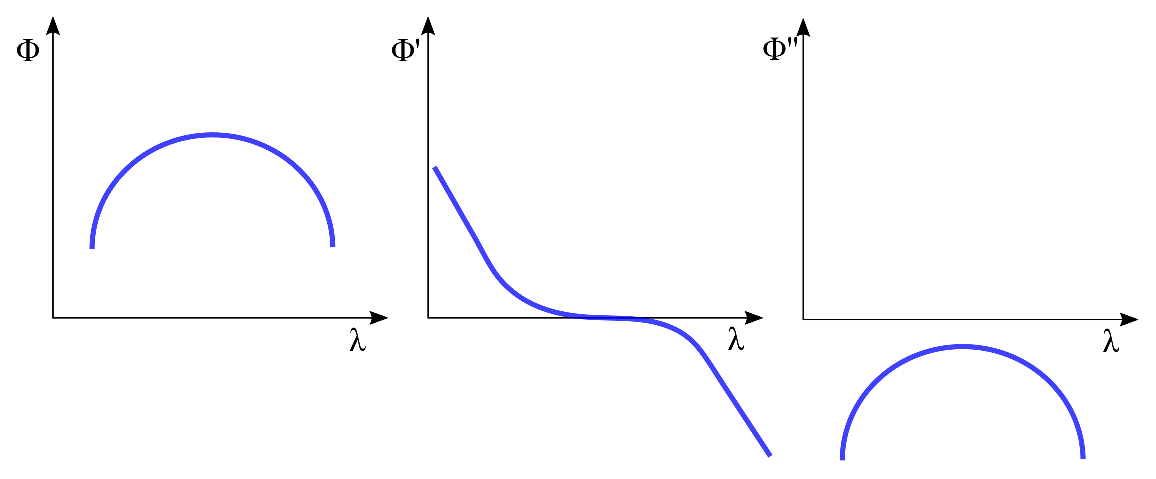
\includegraphics[scale=0.6]{PhiConvex}
    \caption[Connection one to one between $\lambda$ and $a$]{Representation of the convex functional $\Phi[\lambda]$ and its first and second derivative.}
    \label{fig:PhiConvex}
\end{figure}

This argument is  valid for  any pair  of conjugate variables  and it
only depends on  the definition of the  conjugate variables introduced
in Eq. (\ref{relens1}).  It constitutes  the basic content of the DFT
when the relevant variable is the microscopic density operator.

Because the  connection is one  to one,  we may change  variables from
$\lambda$ to $a$.   However, the average $a$ is given  by a derivative
and such a  change of variables implies a loss  of information.  As we
know from the usual treatment in Thermodynamics \cite{Callen1960}, the
correct way to proceed is to  introduce the dimensionless entropy function $S[a]$ of
the given  level of description  as the (minus) Legendre  transform of
the thermodynamic potential in the form
\begin{align}
S[a] &=-\Phi[\lambda[a]]+\lambda[a] a
\label{entropya}\end{align}
The  relation of  this entropy  function $S[a]$  and the  Gibbs-Jaynes
entropy functional  ${\cal S}[\overline{\rho}]$ in  (\ref{entropy}) is
simple. The  former is just  the later  evaluated at its  maximum, the
relevant ensemble (\ref{relens1}). This is
\begin{align}
S[a]={\cal  S}[\overline{\rho}]
\end{align}
Because  the  entropy   $S[a]$  is  the  Legendre   transform  of  the
thermodynamic  potential  $\Phi[\lambda]$,  we have  the  relationship
conjugate to (\ref{cg1})
\begin{align}
  \frac{\partial S}{\partial a}&=\lambda
\label{e3}
\end{align}


\section{The dynamics}\label{Sec:Grabert}
In general it is possible to derive the evolution equation for a given
dynamic  variable  by  using  the technique  of  projection  operators
\cite{Kawasaki1973a,Grabert1982}. The projection operator method can be
understood, at its most fundamental level  as a way to approximate the
actual time dependent ensemble, which is the solution of the Liouville
equation, with a relevant  ensemble of the form (\ref{relens1}),
plus  a correction,  which  is the  responsible  for the  irreversible
behaviour. We  summarize   in  the   rest  of   this  section   the
time-dependent  projection  operator  technique as  presented  in  the
classical  textbook  by Grabert  \cite{Grabert1982}.   

The  aim is  to
derive equations of motion for  the time dependent average $a_i(t)$ of
the set of relevant variables $\hat{A}_i(z)$. The time dependent average
is
\begin{equation}
  a_i(t)={\rm Tr}[\rho_t\hat{A}_i]
  \label{ave}
\end{equation}
where $\rho_t$ is
the nonequilibrium solution of the Liouville equation. As it is shown
in  \cite{Grabert1982},  for  isolated systems  with a time-independent
Hamiltonian,  the   averages  (\ref{ave})  evolve  according   to  the
following closed exact equation

\begin{equation}
\frac{\partial }{\partial t} a_i(t)
= v_i(t) + \int_0^t dt' \sum_j K_{ij}(t,t') \lambda_j(t')
\label{ex}
\end{equation}
The reversible term is given by
\begin{equation}
v_i(t) = {\rm Tr}[\overline{\rho}_t  iL \hat{A}_i]
\label{vit}
\end{equation}
where $iL$ is the Liouville operator (\ref{iL})

The  relevant
ensemble $\overline{\rho}_t$  is of  the form (\ref{relens1}),  with a
time   dependent  conjugate   variable  $\lambda(t)$.   The  conjugate
variables  $\lambda$ are  selected in  such  a way  that the  averages
$a(t)$ of the  real and of the relevant ensemble  coincide.  Note that
if   only  the   reversible  term   $v_i(t)$  would   be  present   in
Eq. (\ref{ex}), we would be  approximating the actual ensemble that it
is a  solution of the Liouville  equation with a relevant  ensemble of
the form (\ref{relens1}) where the conjugate field $\lambda(t)$ is now
a function of time.  The error  in this approximation is, in fact, the
memory term which describes  irreversible behaviour.  The irreversible
term in Eq. (\ref{ex}) involves the memory kernel
\begin{equation}
K_{ij}(t,t') =
{\rm Tr}[\overline{\rho}_{t'} 
\left({\cal Q}_{t'} iL\hat{A}_j\right) G_{t't}
\left({\cal Q}_{t } iL\hat{A}_i\right)]
\label{ker}
\end{equation}
where   the  Kawasaki-Gunton   projection  operator   ${\cal  Q}_{t'}$
\cite{Kawasaki1973a,  Grabert1982}  applied  to an  arbitrary  function
$\hat{F}(z)$ is
\begin{eqnarray}
{\cal Q}_{t'}\hat{F}(z)& = &\hat{F}(z)- {\rm Tr}[\overline{\rho}_{t'} \hat{F}]
\nonumber\\
&-&\sum_i(\hat{A}_i(z)-a_i(t'))\frac{\partial }{\partial a_i(t')}
{\rm Tr}[\overline{\rho}_{t'} \hat{F}]
\label{Q}
\end{eqnarray}
Finally, the time ordered projected propagator $G_{t't}$ is given by formal series
\begin{eqnarray}
G_{t't}&=&1
+\sum_{n=1}^\infty \int_{t'}^tdt_1\cdots\int_{t'}^{t_{n-1}}dt_n
 iL{\cal Q}_{t_n}\cdots  iL{\cal Q}_{t_1}
\nonumber\\
&=&T_-\exp\left\{\int_{t'}^t dt''  iL{\cal Q}_{t''}\right\}
\end{eqnarray}
Eq.   (\ref{ex}) is  a closed  exact equation  for the  time dependent
averages $a(t)$.  The only assumption  taken in deriving (\ref{ex}) is
that the initial  ensemble to be used in the  Liouville equation is of
the relevant form.  This is, it is assumed that  the only knowledge at
the initial  time is the value  of the average $a(0)$  and, therefore,
the  least   biased  initial   ensemble  is   of  the   relevant  form
(\ref{relens1}).  Therefore, the time  dependent average $a(t)$ of the
relevant variables $\hat{A}(z)$  is computed with the  solution of the
Liouville equation $\rho_t(z)$  with an initial condition  which is of
the relevant  form.  The relevant  ensemble is a functional  of $a(t)$
through  $\lambda(t)$.   The kernel  becomes  a  functional of  $a(t)$
through the relevant  ensemble.  

Although Eq.  (\ref{ex})  is a closed
equation it is an integro-differential  equation which is difficult to
treat  in   general.   Nevertheless,  the  exact   transport  equation
(\ref{ex}) can  be approximated by  a memory-less equation  whenever a
clear separation  of time scales  exists between the evolution  of the
averages and  the decay of  the memory kernel. Under  this assumption
and the  neglect of terms of  order ${\cal O}( iL\hat{A}^3)$,  assumed to be
small due to  the slowness of the relevant variables,  one obtains the
Markovian equation \cite{Grabert1982}
\begin{equation}
\dot{a}_i(t) = v_i(t) + \sum_j D_{ij}(t) \lambda_j(t)
\label{ex2}
\end{equation}
where  the  dissipative matrix  is  given  by  the Green-Kubo  formula
\begin{equation}
D_{ij}(t)=\int_0^{\Delta t} dt'\left\langle 
{\cal Q}_t iL\hat{A}_j\exp\{iLt'\}{\cal Q}_t iL\hat{A}_i
\right\rangle^{\lambda(t)}
\label{dij}
\end{equation}
Here,  $\Delta t$ is  a  time large  compared  to the  decay  time of  the
correlation  integrand  but  short  in  front of  the  time  scale  of
evolution of  the relevant variables.  The  dissipative matrix depends
in general  on the  relevant variables  through the  relevant ensemble
and, as such, it is a function of time.  The dissipative matrix is, to
the  extent that  the  Markov property  holds,  positive definite  and
satisfies Onsager's reciprocity \cite{Grabert1982}.

It is straightforward  to show that the  dynamic equations (\ref{ex2})
have  as  a  Lyapunov   function  the  entropy  (\ref{entropya})  and,
therefore,   the   dynamics   complies   with  the   Second   Law   of
Thermodynamics.  The  equations (\ref{ex2})  predict the decay  of any
initial value  of the  average of the  relevant variables  towards its
unique equilibrium  values. Forced situations may  be treated
with the present  formalism \cite{Grabert1982} but we  do not consider
them here for simplicity.


\section{Conclusions}



%-----------------------------------------------------------------
%CHAPTER 2
%-----------------------------------------------------------------
\chapter{Coarse hydrodynamics theory for liquids near solids}\label{Chap:Theory}
\markboth{Coarse hydrodynamics theory for liquids near solids}{}
\epigraph{\textit{Le temps est une invention du mouvement. Celui qui ne bouge pas ne voit pas le temps passer.}}{Métaphysique des tubes \\ AMÉLIE NOTHOMB}
\section{Introduction}
As it was mentioned in the Introduction, Density Functional Theory (DFT) is a successful and well-established theory for the study of the structure of simple and complex fluids at equilibrium. The theory has been generalized to dynamical situations when the underlying dynamics is diffusive as in, for example, colloidal systems. However, there is no such a clear foundation for Dynamic DFT (DDFT) for the case of \textit{simple} fluids in contact with solid walls. In this chapter, we derive DDFT for simple fluids by including not only the mass density field but also the momentum density field of the fluid. The standard projection operator method based on the Kawasaki-Gunton operator is used for deriving the equations for the average value of these fields. 

%The solid is described as featureless under the assumption that all the internal degrees of freedom of the solid relax much faster than those of the fluid (solid elasticity is irrelevant). 
%The fluid moves according to a set of {\em non-local} hydrodynamic equations that include explicitly the forces due to the solid. 
%These forces are of two types, reversible forces emerging from the free energy density functional, and accounting for impenetrability of the solid, and irreversible forces that involve the velocity of both the fluid and the solid. 
%These forces are localized in the vicinity of the solid surface. The resulting hydrodynamic equations should allow one to study dynamical regimes of simple fluids in contact with solid objects in isothermal situations.
We consider a fluid in contact with a 
large  spherical  solid  particle  in  order  to  address  fluid-solid
interactions.   In  usual DFT  approaches,  a  solid wall  is  usually
represented with  an {\em  external hard  potential}.  In  the present
description, a solid  wall is treated with  a coarse-grained procedure
in which  the atoms of the  wall are eliminated from  the description,
under the assumption that any elastic (or any other) degree of freedom
of the  solid is much faster  than the time scales  of the surrounding
fluid.  The  density functional that  emerges now depends not  only on
the density  field of the fluid  but also on the  overall CG variables
that we use to describe the solid.  For simplicity, we focus on a particularly simple particle shape, a solid spherical particle.  By considering the interaction of a  fluid with a solid sphere, we  may address the issue
of total momentum  conservation that may become rather  obscure if one
considers ``planar walls with infinite mass''.  Of course, many of the
results that we obtain will be  easily transferred to planar walls, as
limits in which the  mass and the radius of the  solid sphere are both
very large.   In addition, we  take a spherical particle  because then
only the  position and  momentum of  the center of  mass of  the solid
particle is required in order  to have a coarse-grained description of
the solid.  For non-spherical particles,  it is necessary, in general,
to include also the orientation  and angular velocity of the particle,
as this is expected to play an important role in the dynamics.  Still,
even in the spherical particle case,  it may be important to introduce
angular velocity in order to  have accurate results.  However, for the
sake of simplicity and presentation  of the basic results, we restrict
ourselves in this paper to the simplest case without angular variables
for the  solid particle. Also, and  for the sake of  simplicity, we do
not  consider the  intrinsic spin  of the  fluid, that  may become  an
important        relevant         variable        at        nanoscales
\cite{Hansen2009,Hansen2011a}.

The main result of this chapter is a set of dynamic equations that
govern the non-equilibrium \textit{averages} of hydrodynamic variables
and  the time-dependent  position  and momentum  of  the sphere.   The
dynamic equations  are of the form  of \textit{non-local} hydrodynamic
equations  for  the mass  and  momentum  density fields  coupled  with
Newton's  laws for  the center  of mass  of the  solid particle.   The
coarse-grained forces between the fluid  and the solid have reversible
and  dissipative contributions,  both localized  in a  boundary region
near  the  solid surface.   The  hydrodynamic  equations obtained  can
describe  the structuring  of the  fluid near  the solid  particle and
non-local flow effects that may be important at nano scales.

The  present  theory  is   both,  i)  a
generalization  of density  functional  theory  to dynamic  situations
\textit{in simple  fluids} (fluids that obey  a Hamiltonian dynamics),
and ii) a full description,  at the coarse-grained hydrodynamic level,
of the solid-wall interactions.  The theory describes hydrodynamics at
scales  where the  molecular structure  of the  fluid is  apparent. At
these   scales   the   concept    of   boundary   condition   is   not
applicable. Instead, the interaction of  the fluid with the solid wall
is described with  reversible and irreversible forces  confined at the
vicinity of the wall.

Because  of the  two  aspects of  the present  theory  that have  been
already mentioned, i.e i) non-local hydrodynamics and ii) interactions
with solid walls, we discuss previous  work in these two areas in what
follows.

\subsection{Non-local hydrodynamics}
This   chapter    relies   on   the   pioneering    work   by   Piccirelli
\cite{Piccirelli1968}  who, following  Robertson \cite{Robertson1966},
derived  hydrodynamic   equations  explicitly  from   the  microscopic
dynamics  of  the fluid  system.   The  resulting   exact  hydrodynamic  equations
contained  non-local  transport  coefficients   defined  in  terms  of
Green-Kubo formulae.  In  similar terms, Grossmann \cite{Grossmann1970}
presented a derivation of non-local  hydrodynamics of simple fluids by
using  essentially  the  same  ideas behind  the  projection  operator
technique.    While   the    theory   provided   non-local   transport
coefficients, no connection was made in these early works with Density
Functional Theory,  which was not  yet developed in those  days.  Such
non-local  versions  for hydrodynamics  are  necessary  when the  flow
fields vary rapidly in space,  in the range of molecular correlations.
The  probing of  nanoscales in  MD simulations  has demonstrated  this
point                         very                        convincingly
\cite{Zhang2004,Hansen2007,Todd2008a,Hansen2011}.

\subsection{Fluid-solid  interactions}
Usually, at the hydrodynamic level  of description, the interaction of
a fluid with a solid is described through boundary conditions. Seminal
work  on  the understanding  of  boundary  conditions as  irreversible
interfacial processes  was given  by Bedeaux,  Albano, and  Mazur, who
introduced  interfacial  transport   coefficients  entering  into  the
boundary       conditions      \cite{Bedeaux1976}.        While      a
fluctuation-dissipation   theorem   was   formulated  for   the   slip
coefficient  \cite{Bedeaux1977},  which  could suggest  a  microscopic
evaluation  of  the  interfacial  boundary coefficients  in  terms  of
molecular dynamics, it  was not until the contribution  by Bocquet and
Barrat  that microscopic  expressions for  the interfacial  mechanical
\cite{Bocquet1994}  and   thermal  \cite{Barrat2003}   slip  transport
coefficients were given.   This work was a  conceptual breakthrough in
the extensive field of flow slip at solid surfaces.  However, a debate
was  initiated  by  Petravic  and  Harrowell  \cite{Petravic2007}  who
pointed out  that the  Green-Kubo expression  proposed by  Bocquet and
Barrat provides  not an intrinsic  solid-fluid property but  rather it
depends on the geometry of the setup. This is due to the fact that the
original expression reflects the total  fluid friction for shear flow,
including the slip friction at both  interfaces as well as the viscous
friction  in   the  fluid  \cite{Hansen2011,Kannam2011}.    Hansen  et
al. \cite{Hansen2011} propose to look at a thin slab of fluid near the
wall  and propose  a phenomenological  Langevin equation  relating the
velocity of the  center of mass of  the fluid slab and  the force that
the wall exerts on the slab. The friction coefficient may be computed
from  equilibrium  MD  simulations  by  comparing  the  velocity-force
correlation to the velocity-velocity correlations of the slab. Another
recent approach has considered a Generalized Langevin Equation for the
velocity of a  single atom of the fluid near  a wall \cite{Huang2014}.
Recent  work  by   Ramos-Alvarado  et  al.   \cite{Ramos-Alvarado2016}
compares the above different approaches and concludes that simulations
are  very  sensitive  to  post-processing  issues,  leaving  the  story
somewhat inconclusive.

Our  theoretical approach  is not  restricted to  parallel flow  (i.e.
fluid   slabs)  as   is  typically   considered  in   simulation  work
\cite{Bocquet1994,Petravic2007,Hansen2011,Kannam2011,Ramos-Alvarado2016}.
Most derivations of  Green-Kubo expressions for friction  are based on
linear response theory where the  Hamiltonian is slightly perturbed by
an external  forcing \cite{Bocquet1994,Huang2014}.   We follow  here a
different  approach  in  obtaining   directly  the  full  hydrodynamic
equations from the  microscopic dynamics.  In this  way, the transport
coefficients  that  we obtain  are  the  ones  that really  enter  the
equations  of hydrodynamics  in  any general  flow configuration,  not
limited to homogeneous isotropic flat walls.

Note that  all the  mentioned work  on MD  simulations is  directed to
compute  the  transport  coefficients  that appear  in  slip  boundary
conditions.  When one descends to  the nanoscale, however, the picture
of the effect  of the solid-fluid interactions in terms  of a boundary
condition on an idealized surface  is questionable.  For the scales in
which nanostructure is  visible, e.g.  layering near the  wall, we aim
at  describing  the  fluid solid  interaction  through  coarse-grained
forces that extend  in a short range from the  solid. \Note{No lo entiendo:An early attempt
to use a ``friction field''  appeared in Ref. \cite{Sokhan2002}.  Only
when the  fluid is  macroscopic, we  would expect  these forces  to be
treated as  singular forces such that  its effect can be  described as
truly boundary  conditions on  the fluid. } Recently, Camargo et al. \cite{CamargoBC2018} describe how the present theory gives rise to boundary conditions when the flows are macroscopic.

A precursor of the work presented in this chapter can be found in \cite{Cukier1980}.  that considered a Brownian
hard  sphere in  a  sea of  small  hard spheres  and  used both,  Mori
projection  operator  and  kinetic   theory,  to  derive  hydrodynamic
equations  coupled to  the motion  of the  Brownian particle  (without
boundary conditions).   Our method is  more general in  that continuum
pair-wise   potentials   are   allowed   for,   and   the   non-linear
Kawasaki-Gunton  projection operator  \cite{Kawasaki1973a} is  used for
the   coarse-graining   procedure   instead  of   the   simpler   Mori
projector \cite{Huang2014},   the   latter   being  limited   to   near
equilibrium linear  equations of motion \cite{Grabert1982}.   A theory
of  coarse-graining based  on  the Kawasaki-Gunton  projector gives  a
universal structure based on  the usual thermodynamic potentials.  The
use  of  the  Kawasaki-Gunton  projector  allows  us  to  express  the
reversible  part of  the dynamics  in a  way that  generalizes Density
Functional Theory to moving fluids.

Finally, Cadusch et al.  \cite{Cadusch2008}  show   that  the  use  of  a
non-local translation invariant kernel is not exempt  of problems in high
density fluids in strong nanoconfinement. They state: ``the fundamental
theoretical  challenge  that  remains   is  to  include  the  position
dependence  into   the  kernel   so  that   it  becomes   a  genuinely
inhomogeneous function  of space and  also to appropriately  model the
boundary conditions at the  fluid–wall interface, including stick/slip
boundary conditions.'' The present work addresses this challenge.


\section{The system and the relevant variables}
In this section we use the ToCG described in the previous chapter for describing hydrodynamically a liquid near a solid. 
Consider a liquid system of $N$ monoatomic molecules described
with the position and momenta of  their center of mass.  The molecules
are allowed to move through  space unrestrictedly. To avoid the issues
of  an infinite  number  of particles  required  in the  thermodynamic
limit, and to make closer contact with molecular dynamics simulations,
we simply  assume that  the system  has periodic  boundary conditions.
Interacting with that sea of liquid molecules there is a group of $N'$
bonded atoms forming  what we would understand at a macroscopic level
as a solid object of spherical shape. \Note{By considering the interaction of a liquid with a solid sphere, we may address the issue of total momentum conservation that may become rather obscure if one considers "planar walls with infinite mass".}
In addition, we take a solid sphere because then only the position and the momentum of the center of mass is required in order to have a coarse-grained description of the solid sphere. For non-spherical particles, it is necessary, in general, to include also the orientation  and angular velocity of the sphere, as this is expected to play an important role in the dynamics. 
Still, even in the spherical object case, it may be important to introduce angular velocity in order to have accurate results. 
However, for the sake of simplicity and presentation of the basic results, we restrict ourselves in this paper to the simplest case without angular variables for the solid sphere.  


At the microscopic level the system is described  by the set of
as this is expected to play an important role in the dynamics. Still, all  positions  ${\bf  q}_i$  and  momenta  ${\bf  p}_i=m_i{\bf  v}_i$
($i=1,\cdots,N$) of the liquid atoms plus the positions ${\bf q}_{i'}$
and  momenta ${\bf  p}_{i'}=m_{i'}{\bf v}_{i'}$  ($i'=1,\cdots,N'$) of
the atoms  of the solid  sphere.  For  compactness we will  denote the
microstate in either  of the following forms $z$  or ${q,p,q',p'}$. We
will distinguish  with a prime  the labels of  the atoms of  the solid
sphere from the  unprimed labels of the liquid  atoms.  The microstate
of  the  system  evolves  according to  Hamilton's  equations  with  a
Hamiltonian given by
\begin{eqnarray}
H(z) &=& \sum^N_i \frac{p_i^2}{2m_i} + \sum^{N'}_{i'} \frac{p_{i'}^2}{2m_{i'}}
+ U(z)
\label{H}
\end{eqnarray}
where the potential energy $U(z)$ is given by
\begin{align}
U(z)&=  V^{f}(q)+ V^{fs}(q,q')+ V^{s}(q')
\end{align}
We  assume   for  simplicity  a  pair-wise   potential  energy,  where
$V^{f}(q)=\frac{1}{2}\sum^{{NN}}_{i   j}\phi^{ll}_{ij}$   is   the
potential  of  interaction  between   liquid  atoms,  $  V^{ls}(q,q')=
\sum^{NN'}_{ii'}\phi^{ls}_{ii'}$  is  the   potential  of  interaction
between   liquid   atoms   and   solid   atoms,   and   $   V^{s}(q')=
\frac{1}{2}\sum^{{N'N'}}_{i' j'}\phi^{ss}_{i'j'}$ is the potential
of  interaction  between   the  atoms  of  the   solid  object.   Self
interaction of  the atoms  is not  considered, so  $\phi_{ii}=0$, etc.
There are  no external conservative  potentials acting on  the system,
although  they can  be  easily  introduced. We  do  not consider  such
external potentials  in order to  transparently discuss the  issues of
momentum conservation.

Note that at a microscopic level we do not have boundaries of
  any kind, we only have particles interacting with particles in free
(periodic) space.  In lab  situations, typically, liquids are contained
in flasks and other type of  solid objects that prevent the liquid from
leaking.  We could model a spherical  flask containing a liquid in very
much  the same  way  as we  are  going to  treat  the solid  spherical
particle  surrounded  by  the  (possibly  infinite  in  extension,  or
periodic)  liquid. A solid is
  regarded as a collection of  bounded atoms (that is, their relative
distances  do  not  increase  without   bound)  that  are  moving  and
vibrating. The spherical  shape of the particle  should be understood,
of course, in a statistical sense.

\subsection{The relevant variables}
We describe the system at a coarse grained level by selecting as
relevant variables the  mass and momentum density fields  of the liquid
and  the   center  of  mass   position  and  momentum  of   the  solid
sphere. These are given by the following set of phase functions 
\begin{align}
  \hat{\rho}_{\bf r}(z) &=\sum^{N}_im\overline{\delta}({\bf r}-{\bf q}_i),
&&\hat{\bf R}(z)=\frac{1}{N'}\sum_{i'}^{N'}{\bf q}_{i'}
\nonumber\\
  \hat{\bf g}_{\bf r}(z) &=\sum^{N}_i{\bf p}_i\overline{\delta}({\bf r}-{\bf q}_i),
&&\hat{\bf P}(z)=\sum_{i'}^{N'}{\bf p}_{i'}
\label{CGvar}
\end{align}
where $\overline{\delta}({\bf r}-{\bf q}_i)$ is a coarse delta function as, for example, a normalized Gaussian.
In these phase  functions, the position ${\bf r}$ plays  the role of a
continuous index labeling  the phase function. The  position ${\bf r}$
may take any value in  $\mathbb{R}^3$, or its periodic counterpart, as
we  do  not  have  any  restriction to  the  possible  motion  of  the
particles. \Pendiente{The hamiltonian (\ref{H}) is also a relevant variable.}

For the sake of simplicity, we do not include orientational degrees of
freedom of the  solid for the time being.  Note  that by selecting the
center of  mass variables of the  solid as the only  ones necessary to
describe the  state of the solid  we are implicitly assuming  that the
remaining  solid  degrees   of  freedom  are  much   faster  than  the
hydrodynamic  fields.   In  particular,  we assume  that  any  elastic
behaviour of the solid is  so rapidly decaying towards its equilibrium
state  that elastic  variables  do  not need  to  be  included in  the
description. Should this assumption be violated, the resulting dynamic
equations (not including  these elastic variables for the solid)
would probably  be non-Markovian.

A word is in order about a  model for the solid that is sometimes used
in  simulation work,  where the  solid  is  assumed to  be made  of
``frozen''  particles that  act  as simple  generators  of forces  not
reacting back  to the presence of  the liquid. In this  case, the solid
should be modeled as a static external field acting on the liquid. The
structure of the theory changes in this case as we will discuss later.

\subsection{The time derivatives of the relevant variables}
The time derivatives  of the coarse variables play  a fundamental role
in the final structure of  the dynamic equations (\ref{ex2}). The time
derivative $  iL\hat{A}$ is  the result of  applying the  Liouville operator
(\ref{iL}) to the relevant variables.  In this section, we discuss the
particular  form of  $  iL\hat{A}$ for  the case  of  selected CG  variables
(\ref{CGvar}). The action of the Liouville operator on the CG variables gives \cite{Espanol2015a}
\begin{eqnarray}
  iL \hat{\rho}_{\bf r}(z) &=& -\boldsymbol{\nabla}\esc\hat{\bf g}_{\bf r}(z)
\nonumber\\
iL  \hat{\bf g}_{\bf r}(z) &=& -\boldsymbol{\nabla}{\cdot} \hat{{\bf K}}_{\bf r}(z)+
\hat{\bf F}^l_{\bf r}(z)
\label{ildens}
\end{eqnarray}
Here, the kinetic stress tensor is 
\begin{align}
  \hat{{\bf K}}_{\bf r} &=\sum^{N}_i{\bf p}_i{\bf v}_i
\overline{\delta}({\bf r}-{\bf q}_i)
\end{align}
and the total  force density $\hat{\bf F}^l_{\bf r}(z)$  on the liquid
is defined as
\begin{align}
  \hat{\bf F}^l_{\bf r}(z) &
=\sum_i^N-\frac{\partial U}{\partial {\bf q}_i}\overline{\delta}({\bf r}-{\bf q}_i)
\label{Frtot}
\end{align}
We may decompose  this force density into the
force that  the liquid exerts on  the liquid plus the  force that the
solid   exerts  on  the   liquid,  this   is,  
\begin{align}
   \hat{\bf  F}^l_{\bf
  r}(z)&=\hat{\bf  F}^{\rm l\to  l}_{\bf r}(z)  +\hat{\bf  F}^{\rm s\to
  l}_{\bf r}(z) 
\nonumber\\
\hat{\bf F}^{\rm l\to l}_{\bf r}(z) &= \sum^{NN}_{ij}\hat{\bf F}_{ij}\overline{\delta}({\bf r}-{\bf q}_i)
\nonumber\\
\hat{\bf F}^{\rm s\to l}_{\bf r}(z) &= \sum^{NN'}_{ij'}\hat{\bf F}_{ij'}\overline{\delta}({\bf r}-{\bf q}_i)
\label{Fr}
\end{align}
where $\hat{\bf F}_{ij'}$ is the force  that atom $j'$ of the solid
exerts on  atom $i$ of  the liquid.   This is, $\hat{\bf  F}^{\rm l\to
  l}_{\bf r}(z)  $ is  the microscopic force  density that  the liquid
exerts on the liquid molecules that are around the point ${\bf r}$ and
$\hat{\bf F}^{\rm s\to l}_{\bf r}(z)$ is the microscopic force density
that the solid object exerts on the liquid at the point ${\bf r}$.

We may write the force that the liquid exerts on the liquid 
\begin{align}
  \hat{\bf F}^{\rm l\to l}_{\bf r}(z) &= \frac{1}{2}\sum^{NN}_{ij}\hat{\bf F}_{ij}
(\overline\delta({\bf r}-{\bf q}_i)-\overline\delta({\bf r}-{\bf q}_j))
\end{align}
where we  have used that  the indices are  dummy. By using  a standard
trick \cite{Schofield1982,Grabert1982}, we  may express the difference
of the Dirac delta functions in terms of a divergence
\begin{eqnarray}
\overline\delta({\bf r}-{\bf q}_i)-\overline\delta({\bf r}-{\bf q}_j)
=&\int_0^1d\epsilon\frac{d}{d\epsilon}
\overline\delta({\bf r}-{\bf q}_j-\epsilon{\bf q}_{ij})
\nonumber\\
=&-\nabla\int_0^1d\epsilon{\bf q}_{ij}
\overline\delta({\bf r}-{\bf q}_j-\epsilon{\bf q}_{ij})
\nonumber\\
\label{trick}
\end{eqnarray}
\Note{Aclarar si es $-\epsilon q_{ij}$ o $\epsilon q_{ij}$.}

The liquid  force density  $\hat{\bf F}^{\rm  l\to l}_{\bf  r}(z)$ can
then be expressed  as the divergence of the  microscopic virial stress
tensor, this is
\begin{align}
\hat{\bf F}^{\rm l\to l}_{\bf r}(z)&=-\boldsymbol{\nabla}{\cdot} \hat{\boldsymbol{\Pi}}_{\bf r}(z)
\nonumber\\
\hat{\boldsymbol{\Pi}}_{\bf r}(z)&\equiv \frac{1}{2}\sum^{N}_{ij}{\bf q}_{ij}\hat{\bf F}_{ij}
\int_0^{1}d\epsilon \overline\delta({\bf r}-{\bf q}_i+\epsilon{\bf q}_{ij})
\label{micfluxes}
\end{align}
The time derivative of the momentum density (\ref{ildens}) becomes
\begin{align}
    iL\hat{\bf g}_{\bf r}(z)
    &=-\boldsymbol{\nabla}\cdot \hat{{\bf K}}_{\bf r}(z) - \boldsymbol{\nabla}\cdot \hat{{\bf     \Pi}}_{\bf r}(z) +  {\bf F}^{\rm s\to l}_{\bf r}(z) \nonumber \\
    &= -\boldsymbol{\nabla}\cdot\left(\hat{{\bf K}}_{\bf r}(z)+\hat{{\bf \Pi}}_{\bf r}(z)\right) +{\bf F}^{\rm s\to l}_{\bf r} \nonumber \\
    &=-\boldsymbol{\nabla}\cdot \hat{\boldsymbol{\sigma}}_{\bf r}+{\bf F}^{\rm s\to l}_{\bf r},
\label{gls}
\end{align}
where     $\hat{\boldsymbol{\sigma}}_{\bf r}(z)=\hat{{\bf K}}_{\bf
r}(z)+\hat{\boldsymbol{\Pi}}_{\bf r}(z)$  is the microscopic stress
tensor of the fluid, this is
\begin{align}
  \hat{\boldsymbol{\sigma}}_{\bf r}=&
\sum^{N}_i{\bf p}_i{\bf v}_i
\overline\delta({\bf r}-{\bf q}_i)\nonumber\\
&+
\frac{1}{2}\sum^{N}_{ij}{\bf q}_{ij}\hat{\bf F}_{ij}
\int_0^{1}d\epsilon \overline\delta({\bf r}-{\bf q}_i+\epsilon{\bf q}_{ij})
\label{sigma}
\end{align}
For the solid object we have that the action of the Liouville operator gives
\begin{align}
    iL\hat{\bf R}(z) &=\frac{\hat{\bf P}(z)}{M}
  \nonumber\\
    iL\hat{\bf P}(z) &=-\int  d{\bf r} \hat{\bf F}^{\rm s\to l}_{\bf r}(z)
   \label{Pfsl}  
\end{align} 

Note  that the  total  momentum,  which is  defined  in  terms of  the
coarse-grained variables as
\begin{align}
  \hat{\bf P}_T&=\int d{\bf r} \hat{\bf g}_{\bf r}(z)+\hat{\bf P}(z)
\end{align}
satisfies $ iL\hat{\bf P}_T=0$ and is, therefore, a conserved quantity
of  the  microscopic   dynamics.   We  have  used   that  $\int  d{\bf
  r}\boldsymbol{\nabla}\esc\hat{\boldsymbol{\sigma}}=0$  due to  Gauss theorem  and the  fact
that at the infinite we assume there are no fluid molecules. A similar
argument holds when the domain of integration is periodic.


Summarizing, the time derivatives of the relevant variables of the system are
\begin{align}
    iL \hat{\rho}_{\bf r}(z) &= -\boldsymbol{\nabla}\esc\hat{\bf g}_{\bf r}(z)
\nonumber\\
iL\hat{\bf g}_{\bf r}(z)
&=-\boldsymbol{\nabla}\cdot \hat{\boldsymbol{\sigma}}_{\bf r}(z)+{\bf F}^{\rm s\to l}_{\bf r}(z) \nonumber \\
    iL\hat{\bf R}(z) &=\frac{\hat{\bf P}(z)}{M}
  \nonumber\\
    iL\hat{\bf P}(z) &=-\int  d{\bf r} \hat{\bf F}^{\rm s\to l}_{\bf r}(z)
   \label{timeDerivatives}  
\end{align}

\section{The relevant ensemble and the grand potential}
In section \ref{Sec:TheEntropy} we obtained that the ensemble which maximizes the Gibbs-Jaynes entropy function (\ref{entropy}) is of the type
\begin{equation}
\overline{\rho}(z) = \frac{1}{Z[\lambda]} \rho_0\exp\{-\lambda\!\cdot\!\hat{A}(z)\}
%\label{relens1}
\end{equation}
When the CG variables are those in (\ref{CGvar}), the relevant ensemble $\bar{\rho}(z)$ takes the form
\begin{eqnarray}
  \overline{\rho}(z)&=&\frac{1}{\Xi[\lambda]}\rho_0\exp\left\{-\beta H_N(z)\right\}
\nonumber\\
&\times&
\exp\left\{-\beta\int d{\bf r}\left(\lambda_\rho({\bf r})\cdot\hat{\rho}_{\bf
    r}(z)+\boldsymbol{\lambda}_g{({\bf r})\cdot}\hat{\bf g}_{\bf r}(z)\right)\right\}
\nonumber\\
&\times&
\exp\left\{-\beta \boldsymbol{\lambda}_{R}\esc\hat{\bf R}(z)
-\beta \boldsymbol{\lambda}_{P}\esc\hat{\bf P}(z)\right\}
\nonumber\\
\label{relensln}
\end{eqnarray}
The   normalization   factor   is  the   $\lambda$-dependent
grand-canonical partition function defined as
\begin{align}
&\Xi[\lambda]
\equiv
 \sum_{N=0}^\infty \frac{1}{N!h^{3N}}
\int dqdp dq'dp'
\nonumber\\
&\times\exp\left\{-\beta H_N-\beta \sum_{i=1}^Nm \lambda_\rho({\bf
    q}_i)-\beta \sum_{i=1}^N{\bf p}_i\esc\boldsymbol{\lambda}_g({\bf q}_i)\right\}
\nonumber\\
&\times\exp\left\{-\beta \boldsymbol{\lambda}_{R}\esc\hat{\bf R}(z)
-\beta \boldsymbol{\lambda}_{P}\esc\hat{\bf P}(z)\right\}
\label{xiln}
\end{align}
where we have introduced the coarse conjugate variables as
  \begin{align}
\lambda_\rho({\bf q}_i)&=
\int d{\bf r}\lambda_{\rho}({\bf r})\overline{\delta}({\bf r}-{\bf q}_i)
\nonumber\\
\boldsymbol{\lambda_g}({\bf q}_i)&=
\int d{\bf r}\boldsymbol{\lambda}_g({\bf r})\overline{\delta}({\bf r}-{\bf q}_i)
  \end{align}
The conjugate fields $\lambda$ of the CG variables (\ref{CGvar}) are fixed by the condition that the averages of the CG variables with the relevant ensemble coincide with the averages $\rho({\bf  r}),{\bf  g}({\bf
  r}),{\bf  R},{\bf  P}$  computed  with  the 
  solution of  the Liouville equation (we omit the time  dependence for simplicity). This conditions can be expressed as in Eqs. (\ref{cg1}) 
\begin{align}
  \rho({\bf r}) &=\frac{\delta \Phi [\lambda]}{\delta \lambda_\rho({\bf r}) }
&&{\bf R} =\frac{\partial \Phi [\lambda]}{\partial \boldsymbol{\lambda}_R }
\nonumber\\
  {\bf g}({\bf r}) &=\frac{\delta \Phi [\lambda]}{\delta \boldsymbol{\lambda}_g({\bf r}) }
&&{\bf P} =\frac{\partial \Phi [\lambda]}{\partial \boldsymbol{\lambda}_P }
\label{rgo}
\end{align}
where the $\lambda$-dependent grand-canonical potential is given, as in Eq. (\ref{PhiLambda}) by
\begin{eqnarray}
  \Phi [\lambda]&\equiv&-k_BT \ln\Xi [\lambda]
\label{oh}
\end{eqnarray}
As we saw in section (\ref{Sec:TheEntropy}), there is a one to one connection between the CG variables and the conjugate ones becasuse the functional $\Phi[\lambda]$ is convex.  
Therefore, the  functionals $\lambda_{\rho}[\rho,{\bf  g},{\bf R},{\bf
  P}]$,   $\boldsymbol{\lambda}_g[\rho,{\bf   g},{\bf  R},{\bf   P}]$,
$\boldsymbol{\lambda}_R[\rho,{\bf      g},{\bf      R},{\bf      P}]$,
$\boldsymbol{\lambda}_P[\rho,{\bf g},{\bf  R},{\bf P}]$ exist  and are
unique.   We  can  therefore   switch  from  the  conjugate  variables
$\lambda$   to  the   relevant   variables  $a$   and  construct   the
corresponding hydrodynamic functional.The   hydrodynamic functional   is    given   by   the   Legendre    transform   of   the $\lambda$-dependent grand canonical potential, this is
\begin{align}
{\cal H}[\rho,{\bf g},{\bf R},{\bf P}] &=
\Phi [\lambda_\rho,\boldsymbol{\lambda}_g,\boldsymbol{\lambda}_R,\boldsymbol{\lambda}_P]
\nonumber\\
& -
\int d{\bf r}\rho({\bf r})\lambda_\rho({\bf r})
-
\int d{\bf r}{\bf g}({\bf r})\cdot\boldsymbol{\lambda}_g({\bf r})
\nonumber\\
&
-\boldsymbol{\lambda}_R\cdot{\bf R}-\boldsymbol{\lambda}_P\cdot{\bf P}
\label{oleg}
\end{align}

Note that the hydrodynamic functional  is the negative of the corresponding entropy (\ref{entropya}) for the present level of description. Therefore, the Eq. (\ref{e3}) must be satisfied.

\begin{align}
  \lambda_\rho({\bf r}) &=-\frac{\delta {\cal H}}{\delta \rho({\bf r}) }
&&  \boldsymbol{\lambda}_R =-\frac{\partial {\cal H}}{\partial {\bf R} }
\nonumber\\
  \boldsymbol{\lambda}_g({\bf r}) &=-\frac{\delta {\cal H}}{\delta {\bf g}({\bf r}) }
&&  \boldsymbol{\lambda}_P =-\frac{\partial {\cal H}}{\partial{\bf P} }
\label{lno}
\end{align}

It is possible to find the explicit expression of $\lambda_{g}({\bf r})$ and $\boldsymbol{\lambda}_{\bf P}$ by performing the momentum integrals in Eq. (\ref{xiln}). Replacing in Eq. (\ref{xiln}) the Hamiltonian (\ref{H}) and the momentum of the solid (\ref{CGvar}) we obtain 
\begin{align}
\Xi[\lambda]
&\equiv
\sum_{N=0}^\infty \frac{1}{N!h^{3N}}
\int dqdpdq'dp'
\nonumber \\
&\times\exp\left\{-\beta U(z)-\beta \sum_{i=1}^Nm\bar{\lambda}_\rho({\bf
    r}_i) -\beta \boldsymbol{\lambda}_{R}\esc\hat{\bf R}(z) \right\}
\nonumber \\
&\times
\exp\left\{-\beta \left(\sum_{i=1}^N\frac{{\bf p}_i^2}{2m_i} + \sum_{i=1}^{N'}\frac{{\bf p}_{i'}^2}{2m_{i'}} \right) - \beta \sum_{i=1}^N{\bf p}_i\esc\boldsymbol{\bar{\lambda}}_g({\bf q}_i) 
-\beta \boldsymbol{\lambda}_P\sum_{i=1}^{N'}{\bf p}_{i'}\right\}
\end{align}
We may group the terms in this way
\begin{align}
\Xi[\lambda]
&\equiv
\sum_{N=0}^\infty \frac{1}{N!h^{3N}}
\int dqdpdq'dp'
\nonumber \\
&\times\exp\left\{-\beta U(z)-\beta \sum_{i=1}^Nm\bar{\lambda}_\rho({\bf
    r}_i) -\beta \boldsymbol{\lambda}_{R}\esc\hat{\bf R}(z) \right\}
\nonumber \\
&\times
\exp\left\{-\beta \sum_{i=1}^N\left(\frac{{\bf p}_i^2}{2m_i} + {\bf p}_i\esc\boldsymbol{\bar{\lambda}}_g({\bf q}_i)\right)\right\}
\exp\left\{-\beta \sum_{i=1}^{N'}\left(\frac{{\bf p}_{i'}^2}{2m_{i'}} + \boldsymbol{\lambda}_P{\bf p}_{i'}\right) \right\}
\end{align}
We perform the Gaussian integrals over momenta by using 
\begin{align}
\int_{-\infty}^{\infty} dx e^{-ax^2+bx}=\sqrt{\frac{\pi}{a}}e^{b^2/4a} 
\end{align}
reaching the following expression 
\begin{eqnarray}
\Xi [\lambda]
&\equiv&
 \sum_{N=0}^\infty \frac{1}{N!}
\int \frac{dq}{\Lambda^{3N}}\frac{dq'}{\Lambda^{3N'}}e^{-\beta U}
\nonumber\\
&\times&\exp\left\{-\beta \sum_{i=1}^N\left(m\lambda_\rho({\bf
    r}_i)-\frac{m}{2}\boldsymbol{\lambda}_{g}^2({\bf q}_i)\right)\right\}
\nonumber\\
&\times&\exp\left\{-\beta \left(\boldsymbol{\lambda}_R\cdot\hat{\bf R}-\frac{M'}{2}\boldsymbol{\lambda}_{P}^2\right)\right\},
\label{xiln2}
\end{eqnarray}
where we have introduced the thermal wavelength 
\begin{align}
\Lambda=\left(\frac{h^2\beta}{2\pi m}\right)^{\frac{1}{2}}
\label{ThermalWave}
\end{align}
Together with Eq. (\ref{rgo}) and Eq. (\ref{oh})
\begin{align}
  \rho({\bf r}) &=\frac{\delta \Phi [\lambda]}{\delta \lambda_\rho({\bf r}) } = \frac{1}{\Xi[\lambda]} \frac{\delta\Xi [\lambda]}{\delta \lambda_{\rho}({\bf r})} = m
  \nonumber\\
  {\bf g}({\bf r}) &=\frac{\delta \Phi [\lambda]}{\delta \boldsymbol{\lambda}_g({\bf r}) } =\frac{1}{\Xi[\lambda]} \frac{\delta\Xi [\lambda]}{\delta \boldsymbol{\lambda_g}({\bf r})} = -m\cdot\boldsymbol{\lambda}_g({\bf r})
 \nonumber\\
  {\bf P} &=\frac{\partial \Phi [\lambda]}{\partial \lambda_P} =\frac{1}{\Xi[\lambda]} \frac{\partial\Xi [\lambda]}{\partial \lambda_P} = -M'\cdot\lambda_P
\end{align}
This leads directly to the explicit form of the following conjugate variables
\begin{align}
 \boldsymbol{\lambda}_g({\bf r}) &= -\frac{{\bf g}({\bf r})}{\rho({\bf r})}=-{\bf v}({\bf r})
\nonumber\\
 \boldsymbol{\lambda}_P &= -\frac{{\bf P}}{M'}
\label{nu}
\end{align}
and allows  one to interpret  these conjugate variables  as (negative)
velocities.  


We may express the gran potential (\ref{oh}) as a sum of two contributions
\begin{align}
\Phi [\lambda]&=  \Phi^{\rm pos}[\mu,\boldsymbol{\lambda}_R]
-\frac{M'}{2} {\boldsymbol{\lambda}_P}^2
\end{align}
where we have defined the following grand potential
\begin{align}
\Phi^{\rm pos}[\mu,\boldsymbol{\lambda}_R]
&\equiv-k_BT\ln
 \sum_{N=0}^\infty \frac{1}{N!}
\int \frac{dq}{\Lambda^{3N}}\frac{dq'}{\Lambda^{3N'}}\nonumber\\
&\times
\exp\left\{-\beta  \left(U-\sum_{i=1}^N m\cdot\mu({\bf
    r}_i)+ \boldsymbol{\lambda}_R\cdot\hat{\bf R}\right)\right\}
\label{xpos}
\end{align}
and the chemical potential per unit mass has been introduced as
\begin{align}
  \mu({\bf r})&\equiv\frac{1}{2}\lambda_g^2({\bf r})-\lambda_\rho({\bf r})
\label{chempot}
\end{align}

Note that the gran potential (\ref{xpos}) is similar to the macrocanonical gran potential of a fluid, except for the presence of the solid degrees of freedom and the corresponding conjugate variable $\boldsymbol{\lambda}_R$. 

\section{The free energy}
The Legendre transform of the gran potential for a simple liquid gives the classic (free energy) density functional and we may pursue the same route in order to define the free energy density functional of a fluid in the presence of a solid sphere. The Legendre transform of the gran potential (\ref{xpos}) is
\begin{align}
  {\cal F}[\rho,{\bf R}]&\equiv  \Phi^{\rm pos}[\mu,\boldsymbol{\lambda}_R]
-\mu({\bf r})\frac{\delta\Phi^{\rm pos}}{\delta\mu({\bf r})}[\mu,\boldsymbol{\lambda}_R] 
-\boldsymbol{\lambda}_R\frac{\partial \Phi^{\rm pos}}{\partial \lambda_R}[\mu,\boldsymbol{\lambda}_R] 
\label{legPrev}
\end{align}
The derivatives we need of the functional (\ref{xpos}) are \Note{(No me salen estas dos expresiones)}
\begin{align}
 \frac{\delta \Phi^{\rm pos}}{\delta \mu({\bf r})}[\mu,\boldsymbol{\lambda}_R]&=-
\langle \hat{\rho}_{\bf r}\rangle^{\mu,\boldsymbol{\lambda}_R}
\nonumber\\
  \frac{\partial \Phi^{\rm pos}}{\partial \boldsymbol{\lambda}_R}[\mu,\boldsymbol{\lambda}_R]&=
\langle \hat{\bf R}\rangle^{\mu,\boldsymbol{\lambda}_R}
\end{align}
where               the                averages               $\langle
\cdots\rangle^{\mu,\boldsymbol{\lambda}_R}$   are  defined   in  these
equations.  The second  derivatives of $ \Phi^{\rm pos}$  are given by
covariances  (see   Eqs.  (\ref{cg1})-(\ref{covariances}))   and  this
implies that $\Phi^{\rm  pos}[\mu,\boldsymbol{\lambda}_R]$ is a convex
function.  Therefore, the  connection between $\langle \hat{\rho}_{\bf
  r}\rangle^{\mu,\boldsymbol{\lambda}_R},       \langle       \hat{\bf
  R}\rangle^{\mu,\boldsymbol{\lambda}_R}$         and        $\mu({\bf
  r}),\boldsymbol{\lambda}_R$ is  one to  one. Note also  that because
the phase functions  $ \hat{\rho}_{\bf r}, \hat{\bf R}$  do not depend
on particle's momenta, we have that the averages are given by
\begin{align}
  \langle \hat{\rho}_{\bf r}\rangle^{\mu,\boldsymbol{\lambda}_R} &={\rm Tr}[\overline{\rho}\hat{\rho}_{\bf r}]=\rho_{\bf r}
\nonumber\\
  \langle \hat{\bf R}\rangle^{\mu,\boldsymbol{\lambda}_R} &={\rm Tr}[\overline{\rho}\hat{\bf R}]={\bf R}
\end{align}
Therefore,  we have  a one  to  one connection  between the  conjugate
variables  $\mu({\bf  r}),\boldsymbol{\lambda}_R$   and  the  averages
$\rho({\bf  r}),{\bf  R}$  of  the  CG  variables.


Finally, we have the free energy functional ${\cal  F}[\rho,{\bf R}]$ of a structured fluid in the presence of a solid sphere as the following Legendre transform
\begin{align}
  {\cal F}[\rho,{\bf R}]&\equiv  \Phi^{\rm pos}[\mu,\boldsymbol{\lambda}_R]
+
\int d{\bf r}\rho({\bf r})\mu({\bf r})-\boldsymbol{\lambda}_R\cdot{\bf R}
\label{leg}
\end{align}
whose derivatives are given by 
\begin{align}
   \frac{\delta {\cal F}}{\delta\rho({\bf r})}[\rho,{\bf R}] &=\mu({\bf r},{\bf R})
\nonumber\\
   \frac{\partial {\cal F}}{\partial{\bf R}}[\rho,{\bf R}] &=-\boldsymbol{\lambda}_R
\label{Fd2}
\end{align}
We can obtain an expression for the  hydrodynamic functional (\ref{oleg}) replacing the terms $\Phi[\lambda]$, $\boldsymbol{\lambda}_g({\bf r})$, $\boldsymbol{\lambda}_P$, and $\lambda_R\cdot{\bf R}$ by the Eqs. (\ref{xpos}), $(\ref{nu})$, and $(\ref{leg})$, respectively. 
\begin{align}
  {\cal H}[\rho,{\bf g},{\bf R},{\bf P}] =& 
  -\int d{\bf r} \rho({\bf r})\lambda_{\rho}({\bf r}) 
  +\int d{\bf r}\frac{{\bf g}^2({\bf r})}{\rho({\bf r})} 
  \nonumber\\
  &- {\cal F}[\rho,{\bf R}] -\int d{\bf r}\rho({\bf r})\mu({\bf r}) + \frac{{\bf P}^2}{2M'}
\end{align}
If we replace $\mu({\bf r})$ by the Eq. (\ref{chempot}) and use (\ref{nu}), we finally arrive to an expression of the hydrodynamic functional ${\cal H}$ which is the sum of a kinetic part and a "potential" part. 
\begin{align}
  {\cal H}[\rho,{\bf g},{\bf R},{\bf P}] &=   
  \underbrace{\int d{\bf r}\frac{{\bf g}^2({\bf r})}{2\rho({\bf r})} +\frac{{\bf P}^2}{2M'}}_{kinetic}
  +\underbrace{{\cal F}[\rho,{\bf R}]}_{\rm potential}
\label{oleg2}
\end{align}
In \Pendiente{Appendix \ref{Ap:Forces}}, $\boldsymbol{\lambda}_R$
is just the  average force on the solid due  to the fluid.  Therefore,
the ``potential''  part ${\cal  F}[\rho,{\bf R}]$ of  the hydrodynamic
functional  (\ref{oleg})  really  acts  as a  potential  energy  whose
negative gradient  gives the actual  force on the sphere.   For future
reference,  we  may also  compute  the  functional derivative  of  the
hydrodynamic functional ${\cal  H}$ with respect to  the density field
with the result
\begin{align}
  \frac{\delta {\cal H}}{\delta\rho({\bf r})}[\rho,{\bf g},{\bf R},{\bf P}] &=    
-\frac{{\bf v}^2({\bf r})}{2}+  \frac{\delta {\cal F}}{\delta\rho({\bf r})}[\rho,{\bf R}]
\end{align}

The free energy functional is translationally invariant, this is
\begin{align}
  {\cal F}[T_{\bf u}\rho,T_{\bf u}{\bf R}]&=  {\cal F}[\rho,{\bf R}]
\label{fa}
\end{align}
where the translation operator applied to any function is defined as
\begin{align}
  T_{\bf u}f({\bf r})&=f({\bf r}+{\bf u})
\end{align}
The  invariance  can be  shown  by  performing  a suitable  change  of
variables  inside the  phase space  integrals defining  the partition
function.  By taking the derivative with  respect to ${\bf u}$ in both
sides of Eq.  (\ref{fa}) and  setting afterwards ${\bf u}=0$ we obtain
the identity
\begin{align}
  \int d{\bf r}\frac{\delta {\cal F}}{\delta \rho_{\bf r}}
\boldsymbol{\nabla}\rho_{\bf r}&+\frac{\partial {\cal F}}{\partial {\bf R}}=0
\label{iden1}
\end{align}
This  identity will be  crucial in  order to  show that  total  momentum is
conserved by  the reversible part  of the dynamics.  
\Note{Desde ecuación (55) del paper hasta el final de la sección. En principio no veo que sea necesario añadirlo, pero me queda pensarlo detenidamente.}

\section{The transport equations}
In this section we will obtain the transport equation for a fluid in contact with a solid sphere. In Sec. (\ref{Sec:Grabert}) we obtained an expression for the evolution of the selected variables using the technique of projection operators which consists of an irreversible part and a reversible one. 
\subsection{Exact reversible dynamics}\label{Sec:ExactCont}
In this subsection we consider the reversible part for the case that the CG variables are those in Eqs. (\ref{CGvar}).
For the mass density we have
\begin{align}
\left.\partial_t \rho({\bf r},t)\right|_{\rm rev}
&=  {\rm Tr}[\overline{\rho}_t  iL\hat{\rho}_{\bf r}] 
=-\boldsymbol{\nabla}\cdot {\bf  g}({\bf r},t)
\label{conrho}
\end{align}
where we have used Eq. (\ref{ildens}) and the fact that the relevant
ensemble average of $\hat{\bf g}_{\bf  r}$ is precisely  the momentum
density field ${\bf g}({\bf r},t)$.  On the other hand, and using again the Eq. (\ref{ildens}), the reversible
part of the momentum density evolution equation is
\begin{align}
\left.\partial_t {\bf g}({\bf r},t)\right|_{\rm rev}
&=  {\rm Tr}[\overline{\rho}_t  iL\hat{{\bf g}}_{\bf r}] 
\nonumber\\
&=-\boldsymbol{\nabla}\cdot  {\rm Tr}[\overline{\rho}_t \hat{{\bf K}}_{\bf r}] 
+  {\rm Tr}[\overline{\rho}_t  \hat{\bf F}^{\rm l}_{\bf r}]
\label{grev1}
\end{align}

We will compute the terms of Eq. (\ref{grev1}) taking advantage of the Galilean operator. 


The Galilean operator changes the velocity arguments from ${\bf v}_i\to {\bf v}_i-{\bf v}({\bf q}_i)$ for each $i$ fluid particle, this is
\begin{align}
&  {\cal G}\hat{F}({\bf q}_1,\cdots{\bf q}_N,{\bf p}_1,\cdots{\bf p}_N)
\nonumber\\
=&\hat{F}({\bf q}_1,\cdots{\bf q}_N,{\bf p}_1+m_1{\bf v}({\bf q}_1),\cdots{\bf p}_N+m_N{\bf v}({\bf q}_N))
\end{align}
The intuitive meaning of the Galilean operator is that when applied to a phase function gives how it is seen in a reference frame that moves with the flow field. \Note{Entender bien la forma intuitiva}. Within any trace this is just a change of variables. Therefore, we have the property
\begin{align}
  {\rm Tr}[\bar{\rho}_t\hat{F}] &= {\rm Tr}[({\cal G}\bar{\rho}_t)({\cal G}\hat{F})] \nonumber \\
  \label{Gprop}
\end{align}
The action of the Galilean operator on the relevant variables is
\begin{align}
  {\cal G}\hat{\rho}_{\bf r} &= \hat{\rho}_{\bf r} \nonumber\\
  {\cal G}\hat{g}_{\bf r} &= \hat{g}_{\bf r} + {\bf v}({\bf r})\hat{\rho}_{\bf r} \nonumber \\
  {\cal G}\hat{R}(z) &= \hat{R}(z) \nonumber\\
  {\cal G}\hat{P}(z) &= \hat{P}(z)
\end{align}
Therefore, the action of ${\cal G}$ on the relevant ensemble is \Note{(En el paper aparece $\rho^{eq}$ y no sé de dónde sale...)}
\begin{align}
  {\cal G}\overline{\rho}_t &=
\frac{1}{\Xi[\lambda(t)]}\rho_0
\exp\left\{\beta\int d{\bf r}\mu({\bf r})\hat{\rho}_{\bf r}(z)\right\}
\nonumber\\
&\times
\exp\left\{-\beta \boldsymbol{\lambda}_{R}(t)\esc\hat{\bf R}
-\beta \boldsymbol{\lambda}_{P}(t)\esc\hat{\bf P}\right\}
\label{resrelens}
\end{align}
where  the chemical  potential per  unit mass  has been  introduced in
Eq.  (\ref{chempot}).  \Note{Esta expresión de la colectividad relevante es gaussiana en momento pero el último término hace que sea lineal. ¿Por qué utilizamos el operador galileano si $\bar{\rho}_t$ sigue siendo gaussiana y con término lineal?}
The  action  of the  Galilean  operator on  the
microscopic kinetic stress tensor is
\begin{align}
  {\cal G}\hat{{\bf K}}_{\bf r} &=
\hat{{\bf K}}_{\bf r} 
+{\bf v}({\bf r})\hat{\bf g}_{\bf r}
+\hat{\bf g}_{\bf r}{\bf v}({\bf r})
+{\bf v}({\bf r}){\bf v}({\bf r})\hat{\rho}_{\bf r}
\end{align}
Using (\ref{Gprop}) we have
\begin{align}
  {\rm Tr}[\bar{\rho}_t\hat{{\bf K}}]={\rm Tr}[({\cal G}\bar{\rho}_t)({\cal G}\hat{{\bf K}}_{\bf r})]
\end{align}

By noting that the ensemble (\ref{resrelens}) is Gaussian in momenta, we have finally \Note{No consigo llegar a la siguiente expresión}
\begin{align}
  {\rm Tr}[\overline{\rho}_t \hat{{\bf K}}_{\bf r}] &=
{\bf v}({\bf r}){\bf v}({\bf r}){\rho}({\bf r})+\frac{k_BT}{m}\rho({\bf r})\boldsymbol{\delta}
\label{api}
\end{align}
where $\boldsymbol{\delta}$ is the unit  tensor.  

Now, let us consider the average of the total force density on the liquid, Eq. (\ref{Frtot})
\begin{align}
{\bf F}^l_{\bf r} &\equiv{\rm Tr}[\overline{\rho}_t \hat{\bf F}^l_{\bf r}] =
 \langle \hat{\bf F}^l_{\bf r}\rangle^{\mu,\boldsymbol{\lambda}_R}
\nonumber\\
&=
\frac{1}{\Xi[\mu,\boldsymbol{\lambda}_R]}
 \sum_{N=0}^\infty \frac{1}{N!}
\int \frac{dq}{\Lambda^{3N}}\frac{dq'}{\Lambda^{3N'}}
\left[\sum^{N}_{j}-\frac{\partial U}{\partial {\bf q}_{j}}\delta({\bf r}-{\bf q}_j)\right]
e^{-\beta U}
\nonumber\\
&\times \exp\left\{-\beta  \left( \boldsymbol{\lambda}_R\cdot\hat{\bf R}
-\sum_{i=1}^N m\mu({\bf q}_i)\right)\right\}
\end{align}
where we have  used the definition of the average  with respect to the
relevant ensemble,  after performing the momentum  integrals. Next, we
realize that the  derivative of the Boltzmann factor  is the potential
times the Boltzmann factor itself, this is
\begin{align}
{\bf F}^l_{\bf r}&=
\frac{1}{\Xi[\mu,\boldsymbol{\lambda}_R]}
 \sum_{N=0}^\infty \frac{1}{N!}
\int \frac{dq}{\Lambda^{3N}}\frac{dq'}{\Lambda^{3N'}}
\exp\left\{-\beta  \left(\boldsymbol{\lambda}_R\cdot\hat{\bf R}
-\sum_{i=1}^N m\mu({\bf   r}_i)\right)\right\}
\nonumber\\
&\times k_BT\sum^{N}_{j}\delta({\bf r}-{\bf q}_j)\frac{\partial }{\partial {\bf q}_{j}}e^{-\beta U}
\end{align}
Integrate by parts to obtain
\begin{align}
{\bf F}^l_{\bf r}&=
\frac{1}{\Xi[\mu,\boldsymbol{\lambda}_R]}
 \sum_{N=0}^\infty \frac{1}{N!}
\int \frac{dq}{\Lambda^{3N}}\frac{dq'}{\Lambda^{3N'}}
e^{-\beta U}
k_BT\sum^{N}_{j}-\frac{\partial }{\partial {\bf q}_{j}}\left[\delta({\bf r}-{\bf q}_j)
\exp\left\{-\beta  \left( \boldsymbol{\lambda}_R\cdot\hat{\bf R}
-\sum_{i=1}^N m\mu({\bf q}_i)\right)\right\}\right]
\nonumber\\
&=
\frac{1}{\Xi[\mu,\boldsymbol{\lambda}_R]}
 \sum_{N=0}^\infty \frac{1}{N!}
\int \frac{dq}{\Lambda^{3N}}\frac{dq'}{\Lambda^{3N'}}
e^{-\beta U}
\sum^{N}_{j}\exp\left\{-\beta  \left( \boldsymbol{\lambda}_R\cdot\hat{\bf R}
-\sum_{i\neq j}^N m\mu({\bf   q}_j)\right)\right\}
\nonumber\\
&\times k_BT\left[-\frac{\partial }{\partial {\bf q}_{j}}\delta({\bf r}-{\bf q}_j)
\exp\left\{\beta   m\mu({\bf   q}_j)\right\}\right]
\nonumber\\
&=\frac{k_BT}{m}\boldsymbol{\nabla} \rho({\bf r})
-\rho({\bf r})\boldsymbol{\nabla}\mu({\bf r})
\label{fllr}
\end{align}

By  collecting (\ref{api})  and  (\ref{fllr})  into  the  momentum  density  equation (\ref{grev1}) we obtain
\begin{align}
\left.\partial_t {\bf g}({\bf r},t)\right|_{\rm rev} 
&=-\boldsymbol{\nabla}\cdot\left({\bf v}({\bf r},t)  {\bf g}({\bf r},t)  \right)
-\rho({\bf r})\boldsymbol{\nabla}
\frac{\delta {\cal F}}{\delta\rho({\bf r})}[\rho,{\bf R}]
\label{grev}
\end{align}

In order to obtain the dynamics of the solid variables, we need to compute the average of the total force on the solid ${\bf F}^s$. We may follow identical steps as the case of the total force on the fluid ${\bf F}^f$ and obtain
\begin{align}
{\bf F}^s&={\rm Tr}[\overline{\rho}_t \hat{\bf F}^s]=
 \langle \hat{\bf F}^s\rangle^{\mu,\boldsymbol{\lambda}_R} 
\nonumber\\
&=\frac{1}{\Xi[\mu,\boldsymbol{\lambda}_R]}
 \sum_{N=0}^\infty \frac{1}{N!}
\int \frac{dq}{\Lambda^{3N}}\frac{dq'}{\Lambda^{3N'}}
\left[-\sum^{N'}_{i'}\frac{\partial U}{\partial {\bf q}_{i'}}\right]
e^{-\beta U}
\exp\left\{-\beta  \left(\sum_{i=1}^N m\mu({\bf
    r}_i)+ \boldsymbol{\lambda}_R\cdot\hat{\bf R}\right)\right\}
\nonumber\\
&=
\frac{1}{\Xi[\mu,\boldsymbol{\lambda}_R]}
 \sum_{N=0}^\infty \frac{1}{N!}
\int \frac{dq}{\Lambda^{3N}}\frac{dq'}{\Lambda^{3N'}}
\exp\left\{-\beta  \left(\sum_{i=1}^N m\mu({\bf
    r}_i)+ \boldsymbol{\lambda}_R\cdot\hat{\bf R}\right)\right\}
k_BT\left[\sum^{N'}_{i'}\frac{\partial }{\partial {\bf q}_{i'}}\right]e^{-\beta U}
\nonumber\\
&=
\frac{1}{\Xi[\mu,\boldsymbol{\lambda}_R]}
 \sum_{N=0}^\infty \frac{1}{N!}
\int \frac{dq}{\Lambda^{3N}}\frac{dq'}{\Lambda^{3N'}}
e^{-\beta U}
k_BT\left[-\sum^{N'}_{i'}\frac{\partial }{\partial {\bf q}_{i'}}\right]\exp\left\{-\beta  \left(\sum_{i=1}^N m\mu({\bf
    r}_i)+ \boldsymbol{\lambda}_R\cdot\hat{\bf R}\right)\right\}
\nonumber\\
&=
\frac{1}{\Xi[\mu,\boldsymbol{\lambda}_R]}
 \sum_{N=0}^\infty \frac{1}{N!}
\int \frac{dq}{\Lambda^{3N}}\frac{dq'}{\Lambda^{3N'}}
e^{-\beta U}
\exp\left\{-\beta  \left(\sum_{i=1}^N m\mu({\bf
    r}_i)+ \boldsymbol{\lambda}_R\cdot\hat{\bf R}\right)\right\}
\left[\sum^{N'}_{i'}\frac{\partial }{\partial {\bf q}_{i'}}\right] \boldsymbol{\lambda}_R\cdot\hat{\bf R}
\nonumber\\
&=\boldsymbol{\lambda}_R
\label{lf}\end{align}
This  identity  allows  one  to  interpret  physically  the  Lagrange
multiplier $\boldsymbol{\lambda}_R$ as the  force on the solid sphere.
By  using (\ref{Fd2})  we obtain  that the  total force  on the  solid
sphere is due to the gradient of the free energy functional
\begin{align}
{\bf F}^s&=-\frac{\partial  {\cal F}}{\partial{\bf R}}[\rho,{\bf R}]
\label{Fls}
\end{align}

Therefore, the averages with the relevant ensemble of the solid object variables are
\begin{align}
{\rm Tr}[\overline{\rho}_t  iL\hat{\bf R}] 
&=\frac{\bf P}{M}
\nonumber\\
{\rm Tr}[\overline{\rho}_t  iL\hat{\bf P}] 
&=-\frac{\partial {\cal F}}{\partial {\bf R}}[\rho,{\bf R}]
\end{align}
where we have used the Eq. (\ref{Fls}).

By collecting the  above results, the reversible part  of the dynamics
has the form
\begin{align}
\left.  \partial_t\rho({\bf r})\right|_{\rm rev}&=-\boldsymbol{\nabla}\cdot{\bf g}({\bf r})
\nonumber\\
\left.  \partial_t{\bf g}({\bf r})\right|_{\rm rev}&=-\boldsymbol{\nabla}\cdot\left({\bf g}({\bf r}){\bf v}({\bf r})\right)
-\rho({\bf r})\boldsymbol{\nabla} \frac{\delta {\cal F}}{\delta\rho({\bf r})}[\rho,{\bf R}]
\nonumber\\
\partial_t\left. {\bf R}\right|_{\rm rev}&=\frac{\bf P}{M}
\nonumber\\
\partial_t\left.{\bf P}\right|_{\rm rev}&=-\frac{\partial {\cal F}}{\partial {\bf R}}[\rho,{\bf R}]
\label{rev}
\end{align}
These reversible  equations are exact  as no approximations  have been
made so far. We qualify these  equations as reversible because, as can
be  explicitly  shown,  they   conserve  the  hydrodynamic  functional
(\ref{oleg}), which  is minus the entropy corresponding
  to this level of description.

\subsection{Markovian irreversible dynamics}
While the  reversible part of  the dynamics (\ref{rev}) is  exact, the
irreversible  part  that we  consider  is  approximate
because  we will  assume a  Markovian dynamics.   Under the  Markovian
approximation in which the memory kernel is assumed to decay in a time
scale  short  as compared  to  the  time  scales of  the  hydrodynamic
variables,   the  irreversible   dynamics   is  given   by  the   term
$\sum_jD_{ij}\lambda_j$   in  Eq.   (\ref{ex2}).   Because   the  time
derivatives of  $\rho({\bf r})$ and  ${\bf R}$  are given in  terms of
momenta, which  are relevant variables  themselves, the effect  of the
projection operator in (\ref{Q}) is simply ${\cal Q} iL\rho_{\bf r}=0$
and ${\cal Q}  iL{\bf R}_{\mu}=0$ resulting in  a large simplification
of  the  friction  matrix.   The irreversible  part  of  the  dynamics
$\sum_jD_{ij}\lambda_j$ in Eq. (\ref{ex2}) now takes the form
\begin{align}
\partial_t  \left(
    \begin{array}{c}
\rho({\bf r})\\
\\
{\bf g}({\bf r})\\
\\
{\bf R}\\
\\
{\bf P}
    \end{array}
\right)_{\rm irr}
&=
-\left(\begin{array}{cccc}
  0&0 &0&0\\
\\
0 &\int d{\bf r}'M^{gg}_{{\bf r}{\bf r}'}&0&M^{gP}_{\bf r}\\
\\
  0&0 &0&0\\
\\
0&\int d{\bf r}' M^{Pg}_{{\bf r}'}&0&M^{PP}
\end{array}\right)
\left(    \begin{array}{c}
\frac{\delta {\cal H}}{\delta \rho_{{\bf r}'}}\\
\\
\frac{\delta {\cal H}}{\delta {\bf g}_{{\bf r}'}}\\
\\
\frac{\partial {\cal H}}{\delta {\bf R}}\\
\\
\frac{\partial {\cal H}}{\delta {\bf P}}
    \end{array}
\right)
\label{irr1}
\end{align}
where we have  used (\ref{lno}). The sum over  the continuum ``index''
${\bf  r}$ becomes  an integral.   The domain  of integration  of this
integral  is  $\mathbb{R}^3$,  including  the interior  of  the  solid
sphere. By  using the  results (\ref{lno}),  (\ref{nu}) that  link the
functional derivatives of  the CG Hamiltonian with  respect to momenta
to the velocities, we obtain the following irreversible dynamics
\begin{align}
  \partial_t{\bf g}({\bf r})&=-\int d{\bf r}'M^{gg}_{{\bf r}{\bf r}'}
{\bf v}({\bf r}')-M^{gP}_{\bf r}{\bf V}
\nonumber\\
\frac{d}{dt}{\bf P}(t)&=-\int d{\bf r}' M^{Pg}_{{\bf r}'}{\bf v}({\bf r}')-M^{PP}{\bf V}
\label{IrrMark1}\end{align}
where the matrix elements are  defined in terms of Green-Kubo formulae
as
\begin{align}
  M^{gg}_{{\bf r}{\bf r}'}&=\frac{1}{k_BT}\int_0^{\Delta t} dt\langle 
{\cal Q}  iL\hat{\bf g}_{{\bf r}}(t){\cal Q}  iL\hat{\bf g}_{{\bf r}'}\rangle^\lambda
\nonumber\\
  M^{gP}_{{\bf r}}&=\frac{1}{k_BT}\int_0^{\Delta t} dt\langle 
{\cal Q}  iL\hat{\bf g}_{\bf r}(t){\cal Q}  iL\hat{\bf P}\rangle^\lambda
\nonumber\\
  M^{Pg}_{{\bf r}'}&=\frac{1}{k_BT}\int_0^{\Delta t} dt\langle 
{\cal Q}  iL\hat{\bf P}(t){\cal Q}  iL\hat{\bf g}_{{\bf r}'}\rangle^\lambda
\nonumber\\
  M^{PP}&=\frac{1}{k_BT}\int_0^{\Delta t} dt\langle 
{\cal Q}  iL\hat{\bf P}(t){\cal Q}  iL\hat{\bf P}\rangle^\lambda
\nonumber\\
\label{Ms}
\end{align}
Note that momentum conservation implies that the gain rate of the total momentum
of the fluid is equal to the loss rate of momentum of the particle
\begin{align}
  \int d{\bf r} iL\hat{\bf g}_{\bf r}&=-iL\hat{\bf P}
\label{iLgiLP}
\end{align}
The conservation of momenta then implies the following relationships between
elements of the dissipative matrix
\begin{align}
M^{gP}_{{\bf r}}&=-\int d{\bf r}'M^{gg}_{{\bf r}{\bf r}'}
\nonumber\\
M^{PP}&= - \int d{\bf r}M^{Pg}_{{\bf r}}
\end{align}
and this leads in Eq. (\ref{IrrMark1}) to 
\begin{align}
  \partial_t{\bf g}({\bf r})&=-\int d{\bf r}'M^{gg}_{{\bf r}{\bf r}'}\left({\bf v}({\bf r}')-{\bf V}\right)
\nonumber\\
\frac{d}{dt}{\bf P}(t)&=\int d{\bf r}\int d{\bf r}'M^{gg}_{{\bf r}{\bf r}'}\left({\bf v}({\bf r}')-{\bf V}\right)
\label{IrrMark2}\end{align}
which contain only  the matrix element $M^{gg}_{{\bf  r}{\bf r}'}$ and are
manifestly  Galilean   invariant.   By  using  Eqs.   (\ref{gls})  and
(\ref{Pfsl}) {in} the  definition  of $M^{gg}_{{\bf  r}{\bf r}'}$  in
Eq. (\ref{Ms}),  and inserting  the result in  the equation  of motion
(\ref{IrrMark1}) one obtains
\begin{align}
\left.  \partial_t{\bf g}^\alpha({\bf r})\right|_{\rm irr}&= \boldsymbol{\nabla}_{\bf r}^{\beta}\boldsymbol{\Sigma}^{\alpha\beta}({\bf r}) +\boldsymbol{{\cal S}}^\alpha({\bf r}) 
\nonumber\\
\left.\frac{d}{dt}{\bf P}^\alpha(t)\right|_{\rm irr}&=-\int d{\bf r}'   \boldsymbol{{\cal S}}^\alpha({\bf r}')
\label{Irr}
\end{align}
where the fluid stress tensor is
\begin{align}
  \boldsymbol{\Sigma}^{\alpha\beta}({\bf r})&=
\int d{\bf r}'
\boldsymbol{\eta}^{\alpha\beta\alpha'\beta'}_{{\bf r}{\bf r}'}
\boldsymbol{\nabla}_{{\bf r}'}^{\beta'}{\bf v}^{\alpha'}({\bf r}')
\label{FluidStress}
\end{align}
and the \textit{irreversible surface force density} on the fluid is defined as
\begin{align}
\boldsymbol{{\cal S}}^\alpha({\bf r})=&
-\int d{\bf r}'{\bf G}^{\alpha\alpha'\beta'}_{{\bf r}{\bf r}'}
\boldsymbol{\nabla}_{{\bf r}'}^{\beta'} {\bf v}^{\alpha'}({\bf r}')
\nonumber\\
+\boldsymbol{\nabla}_{{\bf r}}^{\beta}&\int d{\bf r}'{\bf H}^{\alpha\beta\alpha'}_{{\bf r}{\bf r}'}
( {\bf v}^{\alpha'}({\bf r}')-{\bf V}^{\alpha'})
\nonumber\\
-&\int d{\bf r}'
\boldsymbol{\gamma}^{\alpha\alpha'}_{{\bf r}{\bf r}'}( {\bf v}^{\alpha'}({\bf r}')
-{\bf V}^{\alpha'})
\label{Irreversibleforces}
\end{align}
We use Einstein's sum over repeated indices convention (see Appendix \ref{Ap:Notation}).
In   these    expressions   we    have   introduced    the   following
\textit{non-local}  transport   coefficients:  the   viscosity  kernel
$\boldsymbol{\eta}_{{\bf r}{\bf r}'}$ (fourth  order tensor), the slip
kernels ${\bf  H}_{{\bf r}{\bf r}'},{\bf G}_{{\bf  r}{\bf r}'}$ (third
order  tensors), and  the  friction kernel  $\boldsymbol{\gamma}_{{\bf
    r}{\bf  r}'}$ (second  order  tensor).  They  are  defined by  the
Green-Kubo formulae
\begin{align}
  \boldsymbol{\eta}_{{\bf  r}{\bf r}'} &\equiv
\frac{1}{k_BT}\int_0^{\Delta t} dt'\langle 
{\cal Q}_t\hat{\boldsymbol{\sigma}}_{{\bf r}}(t')
{\cal Q}_t\hat{\boldsymbol{\sigma}}_{{\bf r}'}\rangle^{\lambda(t)}
\nonumber\\
{\bf H}_{{\bf r}{\bf r}'}&\equiv\frac{1}{k_BT}\int_0^{\Delta t} dt'
\langle {\cal Q}_t\hat{\boldsymbol{\sigma}}_{{\bf r}}(t')
{\cal Q}_t\hat{\bf F}^{\rm s\to l}_{{\bf r}'}\rangle^{\lambda(t)}
\nonumber\\
{\bf G}_{{\bf r}{\bf r}'}&\equiv\frac{1}{k_BT}\int_0^{\Delta t} dt'
\langle {\cal Q}_t\hat{\bf F}^{\rm s\to l}_{{\bf r}}(t')
{\cal Q}_t\hat{\boldsymbol{\sigma}}_{{\bf r}'}\rangle^{\lambda(t)}
\nonumber\\
\boldsymbol{\gamma}_{{\bf  r}{\bf r}'}&\equiv\frac{1}{k_BT}\int_0^{\Delta t} dt'
\langle 
{\cal Q}_t\hat{\bf F}^{\rm s\to l}_{{\bf r}}(t')
{\cal Q}_t\hat{\bf F}^{\rm s\to l}_{{\bf r}'}\rangle^{\lambda(t)}
\label{GK}
\end{align}
These transport  kernels are state  dependent, i.e.  functions  of the
time  dependent  averages  of  the  relevant  variables,  through  the
dependence of  the relevant ensemble  on these averages.  The explicit
form of the projected currents appearing in these expressions is given
in the Appendix \ref{Ap:Projected}.

\section{The final equations of nano-hydrodynamics} 
By collecting the reversible part  of the dynamics (\ref{rev}) and the
irreversible part  (\ref{Irr}) we  obtain the final  dynamic equations
for the relevant variables
\begin{align}
\partial_t\rho({\bf r})=&-\boldsymbol{\nabla}\cdot{\bf g}({\bf r})
\nonumber\\
\partial_t{\bf g}({\bf r})=&-\boldsymbol{\nabla}\esc{\left({\bf g}({\bf r}){\bf v}({\bf r})\right)}
-\rho({\bf r})\boldsymbol{\nabla}\frac{\delta {\cal F}}{\delta\rho({\bf r})}[\rho,{\bf R}]
\nonumber\\
&+\boldsymbol{\nabla}\esc\boldsymbol{\Sigma}({\bf r})+\boldsymbol{{\cal S}}({\bf r})
\nonumber\\
\dot{\bf R}=&\frac{\bf P}{M}
\nonumber\\
\dot{\bf P}=&-\frac{\partial {\cal F}}{\partial {\bf R}}
-\int d {{\bf r}}\boldsymbol{{\cal S}}({\bf r})
\label{finaleq}
\end{align}
where  the   free  energy  functional  ${\cal   F}[\rho,{\bf  R}]$  is
introduced  in  Eq. (\ref{leg}),  the  velocity  field is  ${\bf  v}({\bf
  r})={\bf  g}({\bf  r})/\rho({\bf  r})$,   the  fluid  stress  tensor
$\boldsymbol{\Sigma}({\bf  r})$ is  given in  (\ref{FluidStress}), and
the irreversible  force $\boldsymbol{{\cal  S}}({\bf r})$ is  given in
Eq. (\ref{Irreversibleforces}).

Eqs.   (\ref{finaleq}), (\ref{GK}),   (\ref{Irreversibleforces}), 
are the  main results of the present  chapter.  They describe
the isothermal non-local  hydrodynamics of a  simple fluid coupled with
the motion of an immersed structureless solid sphere.  These equations
generalize Equilibrium Density Functional Theory for a simple fluid to
non-equilibrium situations in  which the fluid may be  moving around a
solid  sphere.  The  only approximation  that  has been  taken in  the
derivation is the Markovian approximation that neglects memory effects
in the dissipative part of the dynamics.

\Note{Falta desde Let us discuss}

\section{Conclusions}


%-----------------------------------------------------------------
%CHAPTER 3
%-----------------------------------------------------------------
\chapter{Discrete hydrodynamics near solids for planar flows}\label{Chap:Planar}
\markboth{Discrete hydrodynamics near solids for planar flows}{}
\section{Introduction}
In Chapter \ref{Chap:Theory} we  have constructed  from  first
principles a theory  for hydrodynamics in contact with  solids.    Based   on    the   Kawasaki-Gunton   projector
\cite{Kawasaki1973,Grabert1982}, the theory  governs the average value
of the hydrodynamic variables in the  presence of a solid sphere.  The
essential ingredients of  the theory are the  conventional free energy
functional of DFT that governs the  layering of the density field, and
the presence  of irreversible  forces that  are concentrated  near the
solid surface and that are the responsible at the coarse-grained level
of transmitting the  interactions of the solid atoms to  the fluid. 

In   spite   of   its   elegance,   the   theory   as   presented   in
Chapter \ref{Chap:Theory}  cannot yet  be validated  through simulations
for two  reasons.  First,  the amount of  information required  in the
hydrodynamic equations  is exceedingly  large. Non-local  higher order
tensors are  required leading  to an  untractable number  of different
components.   Second, in  order to  compare with  MD simulations,  one
necessarily requires  a discrete version  of such a  theory. Particles
need to  be sorted into  cells in order  to measure ``fields''  in MD.
The  purpose  of  this chapter  is  to  produce  the  discrete
hydrodynamic  equations involving  a  tractable  amount of  measurable
information. The  discrete quantities appearing  in the theory  can be
measured through  equilibrium MD  simulations, and  the theory  may be
then validated by comparing with non-equilibrium MD simulations.  Such
a comparison  allows us to validate  the only assumption on  which the
continuum hydrodynamic equations (\ref{finaleq}) are
based, which  is the  Markovian assumption.   This validation  will be
presented in the following chapters, where  we have observed  that only
for  sufficiently large  discretization cells,  larger than  molecular
sizes,  one observes  Markovian  behaviour.  In  the strict  continuum
limit of  very small cells, a  Markovian theory is unable  to describe
the numerical  results.  
%Therefore, the Markovian  continuum theory of
%Chapter \ref{Chap:Theory} is valid only in  terms  of  coarse  delta
%functions.   This  gives  further
%motivation to introduce the  present discrete hydrodynamic theory with
%its intrinsic built  in length scale given by  the discretization cell
%size.

In  this chapter  we  derive  with  the technique  of  projection
operators the  evolution equations for the  non-equilibrium averages of
the discrete  hydrodynamic variables.   The methodology  follows Refs.
\cite{Espanol2009i,Espanol2009c,DelaTorre2015,EspanolDonev2015}  where
a  set of  discrete hydrodynamic  variables are  introduced through  a
finite  element   basis  function   set.   The   present  work   is  a
generalization of the results  of Ref.  \cite{EspanolDonev2015} in the
presence of solid walls and for the particular case of parallel flows.
The method for deriving the  average evolution of hydrodynamics admits
a straightforward generalization in  terms of fluctuating hydrodynamic
equations as those  in Ref. \cite{EspanolDonev2015}, this  time in the
presence  of  solid  walls,  and will  be  presented  elsewhere.   One
interesting benefit of the discretization methodology that we consider
in this paper is that  the final discrete evolution equations obtained
from first principles are identical to a finite element discretization
of the  continuum equations  (\ref{finaleq}),  once isotropy
and translation invariance along the wall is assumed for the flow.



%In   spite   of   its   elegance,   the   theory presented  cannot yet  be validated  through simulations
%for two  reasons. First,  the amount of  information required  in the
%hydrodynamic equations  is exceedingly  large. Non-local  higher order
%tensors are  required leading  to an  untractable number  of different
%components.   Second, in  order to  compare with  MD simulations,  one
%necessarily requires  a discrete version  of such a  theory. Particles
%need to be sorted into bins in order to measure ``fields'' in MD.  In this chapter we produce  the discrete hydrodynamic
%equations involving a tractable amount of measurable information. The
%discrete quantities  appearing in the  theory can be  measured through
%equilibrium MD  simulations, and the  theory may be then  validated by
%comparing  with non-equilibrium  MD  simulations.   Such a  comparison
%allows  us to  validate the  only  assumption on  which the  continuum
%Dynamic Density Functional Theory given in Chapter \ref{Chap:Theory} is
%based,  which  is  the   Markovian  assumption.   This  validation  conforms the core of the present dissertation  where we  have observed
%that  only for  sufficiently large  discretization cells,  larger than
%molecular  sizes, one  observes  Markovian behaviour.   In the  strict
%continuum limit of  very small cells, a Markovian theory  is unable to
%describe  the numerical  results. Therefore, this  gives  further
%motivation to introduce the  present discrete hydrodynamic theory with
%its intrinsic built  in length scale given by  the discretization cell
%size.

\section{Simpler theory}
The hydrodynamic theory  (\ref{finaleq}) requires
an extremely  large amount of  information in order to  be predictive,
which  is almost  a  contradiction. In particular,
we  need to  know the  transport  coefficients which  are, in  general
non-local,  but  most  dramatically,   tensorial  in  character.   The
Green-Kubo expressions  (\ref{GK}) correlate the  different components
of the  microscopic force vector that  the solid exerts on  the fluid,
and the microscopic stress tensor, defined both in (\ref{sigma}).  The
number  of components  of the  tensorial kernels  is very  large.  The
viscosity  tensor, being  a fourth  order tensor  has in  principle 81
components, but the symmetry of  the microscopic stress tensor reduces
the number  to 36 independent  components.  The tensors  ${\bf G},{\bf
  H}$ are third  order tensors and, on account of  the symmetry of the
microscopic stress  tensor, have 21 independent  components, while the
number of independent  components of the second  order friction tensor
is 9.   Onsager reciprocity reduces  the total  number to 23  which is
still a very large number of components to consider.

For  this reason,  we will  consider a  theory that  is restricted  to
\textit{planar walls}. Specifically, two solid walls made of atoms located at fixed lattice positions enclose our fluid system. The concept of  ``surface'' is subtle  from a
microscopic  point of  view.   In fact,  the solid  is  made of  point
particles that act like centers of  force for the fluid particles. The
concept of  surface of a  solid and its  actual position needs  to be,
therefore, related  to the  interactions between  fluid and  solid, as
discussed in \cite{CamargoBC2018}.

In this chapter we assume that the walls, or rather the interactions felt
by the fluid due to the  walls, are statistically planar and isotropic,
i.e.  invariant under translations in the plane of the wall, and under
rotations around an axis perpendicular to the walls.
In  addition,  we  will  restrict ourselves  to  \textit{planar  flow}
situations  in  which  the  hydrodynamic  flow  depends  only  on  the
coordinate  perpendicular to  the wall,  i.e.  it  is invariant  under
translations tangent to the walls.
In  this way,  the planar  flows  to be considered
include shear  flows (Poiseuille and  Couette, for example)  and sound
wave  propagation perpendicular  to the  walls but  not, for  example,
sound waves that propagate parallel to the walls.

In order to  validate through computer simulations  a continuum theory
like the one presented in Chapter  \ref{Chap:Theory} one needs to follow
three consecutive  steps that  require a  discrete framework.   In the
first  step, equilibrium  MD simulations  should  be run  in order  to
measure  the non-local  transport kernels.   In the  second step,  the
discrete  equations  with  the   measured  kernels  should  be  solved
numerically in order to predict the flow field given a certain initial
velocity  profile.  In  the  third  step, one  should  run a  separate
non-equilibrium MD simulation with  the same initial velocity profile.
By   averaging  over   several   initial  microscopic   configurations
corresponding  to   this  initial   velocity  flow  one   obtains  the
non-equilibrium  average time  evolution  of the  velocity profile  as
measured  from MD.   The  comparison of  the predicted  time-dependent
velocity   profile   with   the    result   obtained   directly   from
non-equilibrium MD simulations allows one to validate the theory.

\textit{All  these  steps  require  the  discretization  of  space  in
  slabs}. In the  first step, this is necessary in  order to deal with
the coarse delta functions that appear  in the force density and stress
  tensor (\ref{sigma}), whose correlations give  rise to the kernels. The
second step  requires a discretization  in order to  solve numerically
Eqs.  (\ref{finaleq}).  Finally, in  the third step the discretization
is required in  order to measure the density and  velocity fields.  It
is  important that  the discretization  in these  three steps  is done
consistently. We have  discussed in Refs. \cite{DelaTorre2015,EspanolDonev2015} how  a method based
on  finite elements  allows one  to construct  the  CG discrete  variables
evolving according  to dynamic  equations that  are consistent  with a
finite  element  discretization of  the  continuum  equations. 


\section{The discrete basis function set}
\label{Sec:DiscreteBasis}
In this chapter, the finite elements are defined in 3D but taking into account the
translation invariance of the flow field along the directions parallel to the walls, as follows.

We bin  the system  in layers  parallel to the  planar walls.   The box
length $L_z$ is  divided in $N_{\rm bin}$ bins labeled  with an index
$\mu$.  Each bin  is a layer or slab of  dimensions $L_x,L_y,\Delta z$
with $\Delta  z=L_z/N_{\rm bin}$.  The  bins are separated  by $N_{\rm
  bin}$ nodes  (actually, nodal  planes) located at  $z_\mu=\mu \Delta
z$,  $\mu=0,\cdots,N_{\rm bin}-1$.   We assume  that we  have periodic
boundary  conditions  in  the  $z$ direction  and,  therefore,  node
$\mu=0$ is equal to the  node $N_{\rm bin}$.  We carefully distinguish
between \textit{nodes} and \textit{bins}: nodes  are points in the $z$
axis, while bins are segments in  this axis.  In 3D, nodes are planes,
while bins are slabs.  As it  will become apparent, from a microscopic
point of view, mass, momentum, and  force densities are defined at the
nodes, while stress is defined at the bins.

We  introduce the  characteristic function  of the  bin $\chi_\mu({\bf
  r})$ that  takes the value  1 if  ${\bf r}$ is  in the bin  and zero
otherwise.  Its explicit form is given by the unit function
\begin{align}
\chi_\mu({\bf r})&=\theta(z_{\mu+ 1}-z)\theta(z-z_\mu)=\chi_\mu(z)
\label{chi}
\end{align}
where $\theta(x)$ is  the Heaviside step function,  $z_{\mu+1}$ is the
position  of the  upper  boundary of  the layer,  and  $z_\mu$ is  the
corresponding  position  of  the  lower boundary  of  the  layer.   The set of characteristic
functions form  a partition of  unity, i.e.  by summing
over all the bins we have
\begin{align}
  \sum_{\mu}^{N_{\rm bin}}\chi_\mu({\bf r})&=1
\label{PartitionUnity}
\end{align}
The volume  integral of the  characteristic function gives  the volume
${\cal V}_\mu$ of the bin
\begin{align}
{\cal V}_\mu&=  \int d{\bf r}\chi_\mu({\bf r})= L_xL_y\Delta z
\end{align}

For each node, we  introduce  a finite element linear  basis  function
$\Phi_\mu({\bf r})$
\begin{align}
  \Phi_\mu({\bf r})=\chi_\mu(z)\frac{z_{\mu+1}-z}{\Delta z}+\chi_{\mu-1}(z)\frac{z-z_{\mu-1}}{\Delta z}
\end{align}
that depends only on the $z$ component of ${\bf r}$. 
The finite element basis functions $\Phi_\mu({\bf r})$ also form a partition of unity, i.e.
\begin{align}
  \sum_\mu\Phi_\mu({\bf r})=1
\label{partition}
\end{align}

We plot  in Figure  \ref{psichi} the  basis function  $\Phi_\mu(z)$ of
node  $\mu$ and  the  characteristic function  $\chi_\mu(z)$ of  bin
$\mu$.
\begin{figure}[h]
  \centering
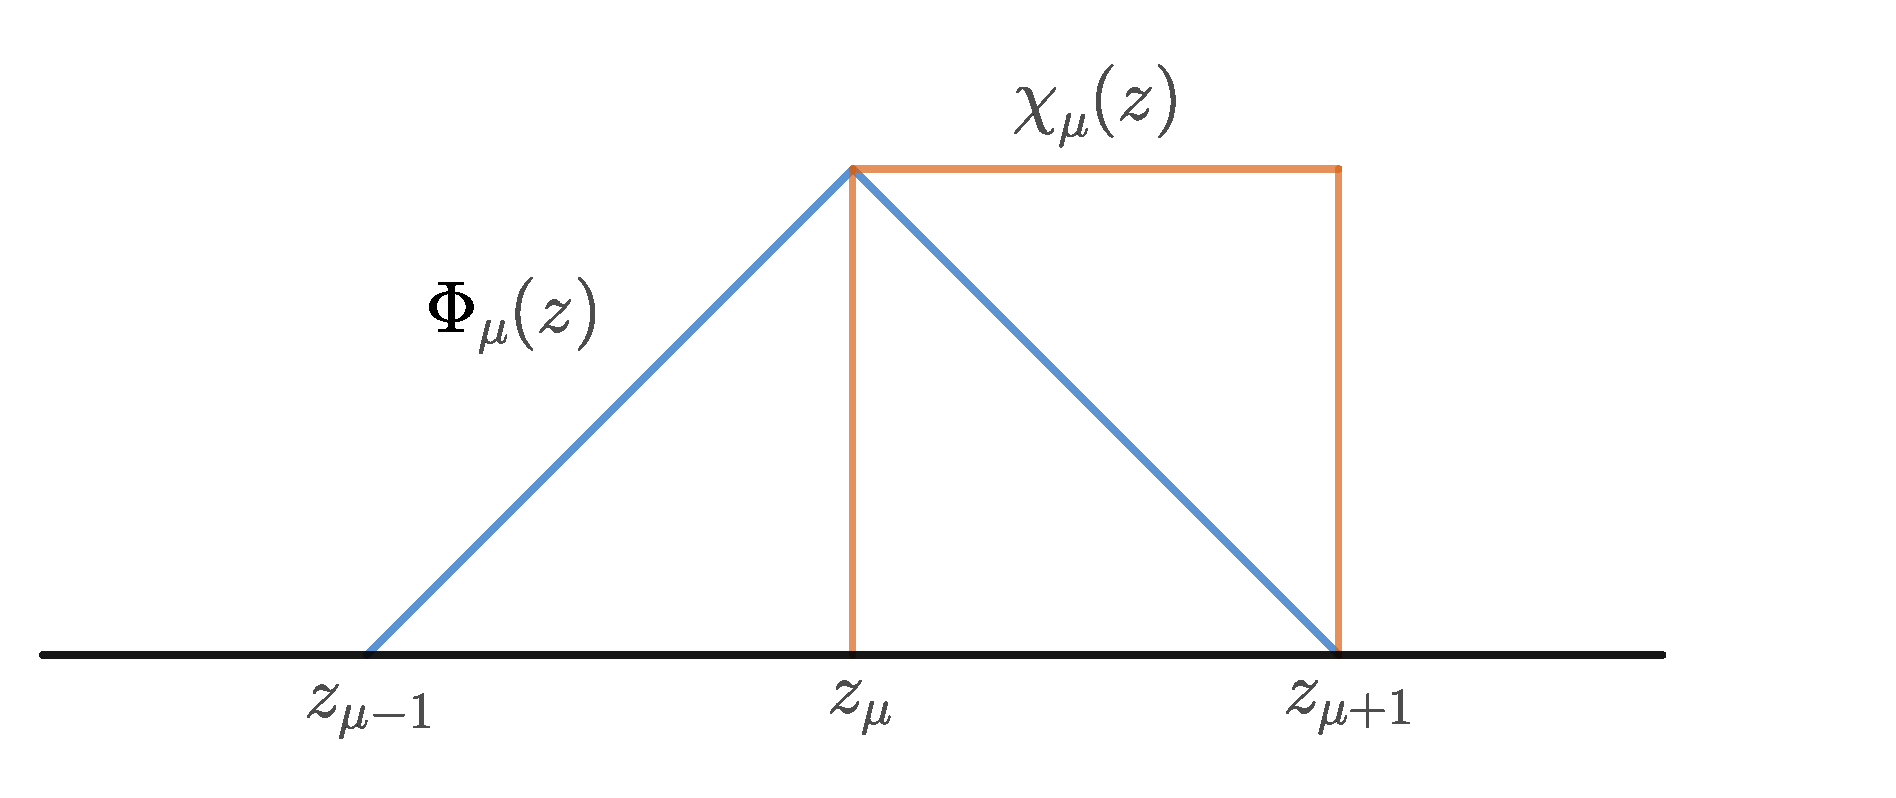
\includegraphics[scale=0.3]{psichi}
\caption{The basis function $\Phi_\mu(z)$ of node $\mu$ (blue) and the characteristic function $\chi_\mu(z)$ of bin $\mu$ (orange).}
\label{psichi}
\end{figure}

The gradient of the basis function is
\begin{align}
\boldsymbol{\nabla}\Phi_\mu({\bf r})&=-\frac{\chi_\mu({\bf r})-\chi_{\mu-1}({\bf r})}{\Delta z}{\bf n}
\label{partialpsi}
\end{align}
where ${\bf n}$ is the unit vector in the normal direction.

Following  Ref. \cite{EspanolDonev2015},  we  now introduce  dual basis  functions
$\delta_\mu({\bf  r})$ and  $\psi_\mu({\bf r})$.   The basis  function
$\delta_\mu({\bf r})$ is used to  discretize a continuum field $v({\bf
  r})$ by defining the discrete values $v_\mu$ according to
\begin{align}
  v_\mu&=\int d{\bf r}v({\bf r})\delta_\mu({\bf r})
\label{Disc}
\end{align}
On the other hand,  the  basis function  $\psi_\mu({\bf r})$ allows one
to construct a continuum field out of a discrete set of values through
interpolation, this is
\begin{align}
  \overline{v}({\bf r}) &=v_\mu\psi_\mu({\bf r})
\label{Cont}
\end{align}
In this chapter, overlined fields indicate  fields interpolated from
a set of discrete values. 
The basis functions are required to
satisfy the biorthonormality condition
\begin{align}
  \int d{\bf r}\delta_\mu({\bf r})\psi_\nu({\bf r})=\delta_{\mu\nu}
\label{biortho}
\end{align}
where $\delta_{\mu\nu}$ is the Kronecker delta. 
It proves convenient to introduce the following 
parenthetical notation for space integrals
\begin{align}
  \llg \cdots\rlg &=\int d{\bf r}\cdots
\label{notation}
\end{align}
and the biorthonormality condition (\ref{biortho}) becomes
\begin{align}
\llg\delta_\mu\psi_\nu\rlg=\delta_{\mu\nu}
\label{biortho2}
\end{align}
We stipulate that the relation between both basis function is linear
\begin{align}
  \delta_\mu({\bf r})&=\sum_\nu M^\delta_{\mu\nu}\psi_\nu({\bf r})
\nonumber\\
  \psi_\mu({\bf r})&=\sum_\nu M^\psi_{\mu\nu}\delta_\nu({\bf r})
\label{dual}
\end{align}
and, then, the biorthonormality condition (\ref{biortho}) implies that 
the matrices are given by
\begin{align}
  M^\delta_{\mu\nu}&= \llg\delta_\mu\delta_\nu\rlg
\nonumber\\
  M^\psi_{\mu\nu}&= \llg\psi_\mu\psi_\nu\rlg
\label{MM}
\end{align}
and these two matrices are inverse of each other.

The biorthonormality  condition ensures the consistency  property that
if  we  discretize  as  in (\ref{Disc})  an  interpolated  field  like
(\ref{Cont}) we get
\begin{align}
  c_\mu&=\int d{\bf r}\delta_\mu({\bf r})\overline{c}({\bf r})
=\sum_\nu\int d{\bf r}\delta_\mu({\bf r})\psi_\nu({\bf r})c_\nu=c_\mu
\end{align}
Therefore,  the   discretization  of   an  interpolated   field  gives
consistently back the original discrete field, and no errors are accumulated in the process.

Let us now specify the actual form of the basis functions.  The finite
element basis  function $\Phi_\mu({\bf  r})$ has an  associated volume
${\cal V}_\mu$ defined as
\begin{align}
  {\cal V}_{\mu}&=\int d{\bf r}\Phi_\mu({\bf r})
\end{align}
and the usual mass matrix of the finite element method is \Note{Entender de forma intuitiva la matriz de masa}
\begin{align}
M^\Phi_{\mu\nu}&=\llg\Phi_\mu\Phi_\nu\rlg  
\label{Mphi}
\end{align}
 and has dimensions of volume. This matrix satisfies 
\begin{align}
\sum_\mu M^\Phi_{\mu\nu} &={\cal V}_\nu
\end{align}
and, by multiplying with the inverse on both sides
\begin{align}
  \sum_\mu {\cal V}_\mu \left[M^{\Phi}\right]^{-1}_{\mu\nu}&=1
\label{sumM}
\end{align}
for all $\nu$.

The discrete  Dirac delta function is  defined in terms of  the finite
element basis function according to \Note{No habría que introducir the discrete coarse delta function?}
\begin{align}
  \delta_\mu({\bf r})\equiv\frac{\Phi_\mu({\bf r})}{{\cal V}_\mu}
\label{DelFE}
\end{align}
The matrices $M^\delta_{\mu\nu}, M^\psi_{\mu\nu}$ defined in (\ref{MM}) are related to
the mass matrix of the finite element basis (\ref{Mphi}) through
\begin{align}
  M^\delta_{\mu\nu}&=\frac{  M^\Phi_{\mu\nu}}{{\cal V}_\mu{\cal V}_\nu}
\nonumber\\
M^\psi_{\mu\nu}&={\cal V}_\mu \left[M^{\Phi}\right]^{-1}_{\mu\nu}{\cal V}_\nu
\label{MdMp}
\end{align}
Given the definition (\ref{DelFE}) for the discrete Dirac delta function,  the interpolant basis function given in (\ref{dual}) takes the form
\begin{align}
  \psi_\mu({\bf r})&
  ={\cal V}_\mu \sum_\nu \left[M^{\Phi}\right]^{-1}_{\mu\nu} \Phi_\nu({\bf r})
\label{PsiFE}
\end{align}
in terms of the finite element basis function set.

\section{The  discrete hydrodynamics equations derived
with the Kawasaki-Gunton projector}
\label{Sec:derivation}
In this section, we present a derivation of the governing equations of
the  dynamics   of  the   non-equilibrium  average  of   the  discrete
hydrodynamic  variables  from first  principles,  i.e.   based on  the
projection operator  technique \cite{Grabert1982}, summarized  in Sec.
\ref{Sec:Grabert} of Chapter \ref{Chap:NESM}.   The coarse-grained variables that we
consider in this chapter are the  total Hamiltonian $\hat{H}(z)$
and the discrete mass and momentum fields, which are defined according to
\begin{align}
\hat{\rho}_\mu&= \sum_i^Nm_i\delta_\mu({\bf q}_i)
\nonumber\\
\hat{\bf g}_\mu&= \sum_i^N{\bf p}_i\delta_\mu({\bf q}_i)
\label{rhogmumic}
\end{align}
No macrocopic variables are assumed fot he solid, because we assumed that it is a very massive wall with definite location.
The  phase  functions (\ref{rhogmumic}),  as  opposed  to  the  microscopic  functions
(\ref{CGvar}) can be  measured directly in a  MD simulation. The
continuum (\ref{CGvar}) and discrete (\ref{rhogmumic}) variables
are connected by
\begin{align}
\hat{\rho}_\mu&= \int d{\bf r}\delta_\mu({\bf r})\hat{\rho}_{\bf r}
\nonumber\\
\hat{\bf g}_\mu&=\int d{\bf r}\delta_\mu({\bf r})\hat{\bf g}_{\bf r}
\label{rhogmumiccont}
\end{align}
The  discrete mass  and momentum  densities are  defined at  the nodal
planes. We see from (\ref{rhogmumic}) that  the mass density at a node
receives a contribution of the mass of fluid molecule $i$ that depends
on  the distance  of  this  molecule to  the  nodal  plane $\mu$,  and
similarly    for   the    momentum.     The   microscopic    variables
(\ref{rhogmumic}) give,  essentially, the number of  particles and the
average velocity of the particles (per  unit volume) that happen to be
``around'' the nodal plane $\mu$.

%By the very
%selection of the  variables (\ref{rhogmumic}) as the  CG variables, we
%are  making a  strong assumption  about  the situations  in which  the
%theory may be applicable.  For  example, the resulting theory will not
%be able to describe situations in which a sound wave is propagating in
%the direction \textit{parallel} to the  walls, because such a wave has
%variations in the parallel direction that cannot be captured by the CG
%variables.  However,  it will  allow us  to discuss  sound propagation
%\textit{perpendicular}  to the  walls.   It is  expected  that the  CG
%variables (\ref{rhogmumic})  will feel the  effects of the walls  in a
%very integrated form, in which the isotropy and translation invariance
%of the  walls will be a  very good approximation.  In  that sense, for
%those situations  in which the  resulting dynamic equations  are valid
%(i.e.  parallel flow),  the assumed isotropy of the  walls is expected
%to be  valid.  
%\Note{No he encontrado la referencia de Donev.} 
%
%The  calculations presented in what follows  are very
%similar to  the ones described  in Ref. \cite{Donev}, except  that the
%present  calculation  deals  with ``canonical''  averages  instead  of
%``microcanonical''  averages  as  in   Ref.  \cite{Donev}.  They  also
%crucially  differ in  that  the present  derivation  accounts for  the
%presence of confining walls.

No macroscopic variables are assumed  for the solid, because we assume
that it  is a very massive  wall with definite location.   By the very
selection of the  variables (\ref{rhogmumic}) as the  CG variables, we
are  making a  strong assumption  about  the situations  in which  the
theory may be applicable.  For  example, the resulting theory will not
be able to describe situations in which a sound wave is propagating in
the direction \textit{parallel} to the  walls, because such a wave has
variations in the parallel direction that cannot be captured by the CG
variables.  However,  it will  allow us  to discuss  sound propagation
\textit{perpendicular}  to the  walls.   It is  expected  that the  CG
variables (\ref{rhogmumic})  will feel the  effects of the walls  in a
very integrated form, in which the isotropy and translation invariance
of the  walls will be a  very good approximation.  In  that sense, for
those situations  in which the  resulting dynamic equations  are valid
(i.e.  parallel flow),  the assumed isotropy of the  walls is expected
to be  valid.  The  calculations presented in what follows  are very
similar to  the ones described  in Ref. \cite{Donev}, except  that the
present  calculation  deals  with ``canonical''  averages  instead  of
``microcanonical''  averages.  They  also
crucially  differ in  that  the present  derivation  accounts for  the
presence of confining walls.

\subsection{The time derivatives}
The time derivatives  of the CG variables  (\ref{rhogmumic}) are given
through the action of the Liouville operator
\begin{align}
i{\cal L}  \hat{\rho}_{\mu}&=\sum_{i=1}^N{\bf p}_i\esc\boldsymbol{\nabla}\delta_\mu({\bf q}_i)
\nonumber\\
i{\cal L}  \hat{\bf g}_{\mu}&=\sum_{i=1}^N{\bf p}_i{\bf v}_i\esc\boldsymbol{\nabla}\delta_\mu({\bf q}_i)
+\hat{\bf F}_\mu
\label{iLMicrhogmu}
\end{align}
In the expression (\ref{iLMicrhogmu}) we see that the momentum density
changes through two different mechanism,  the convective motion of the
particles and  the forces on  the particles.  The total  force density
$\hat{\bf F}_\mu$ felt by the fluid particles at node $\mu$ is
\begin{align}
\hat{\bf F}_\mu&=    \hat{\bf F}^{\rm s\to l}_\mu+  \hat{\bf F}^{\rm l\to l}_\mu
\end{align}
where $  \hat{\bf F}^{\rm  s\to l}_\mu$  is the  force density  on the
fluid  at node  $\mu$ due  to the  solid and  $ \hat{\bf  F}^{\rm l\to
  l}_\mu$ is the force  density on the fluid at node  $\mu$ due to the
fluid. These forces are defined as
\begin{align}
 \hat{\bf F}^{\rm s\to l}_\mu &\equiv\sum_{ij'}\hat{\bf F}_{ij'}\delta_\mu({\bf q}_i)
 \nonumber\\
 \hat{\bf F}^{\rm l\to l}_\mu &\equiv\sum_{ij}\hat{\bf F}_{ij}\delta_\mu({\bf q}_i)
\label{Fbin}
\end{align}
Recall that solid atoms have  primed indices and fluid atoms have unprimed indices.


For future reference,  we express the time derivative  of the discrete
momentum density field  in terms of a discrete stress  tensor. 
The  gradient   of  the  discrete   delta  function  is   given,  from
(\ref{partialpsi}) and (\ref{DelFE}), by
\begin{align}
  \boldsymbol{\nabla}\delta_\mu({\bf r})=-\frac{1}{{\cal V}_\mu}\frac{\chi_\mu(z)-\chi_{\mu-1}(z)}{\Delta z} {\bf n}
\end{align}
This means that the convective part can be expressed in the form
\begin{align}
  \sum_{i=1}^N{\bf p}_i{\bf v}_i\esc\boldsymbol{\nabla}\delta_\mu({\bf q}_i)&=
-\frac{1}{{\cal V}_\mu} \sum_{i=1}^N{\bf p}_i{\bf v}_i\esc{\bf n}\frac{\chi_\mu(z)-\chi_{\mu-1}(z)}{\Delta z}
\nonumber\\ 
\end{align}
For the force due to the fluid we may use the trick
\begin{align}
  \hat{{\bf F}}_\mu^{\rm l\to l}&=  \sum_{ij}^N\hat{\bf F}_{ij}\delta_\mu({\bf q}_i)
\nonumber\\
&=\frac{1}{2}\sum_{ij}^N\hat{\bf F}_{ij}
(\delta_\mu({\bf q}_i)-\delta_\mu({\bf q}_j))
\nonumber\\
&=\frac{1}{2}\sum_{ij}^N\hat{\bf F}_{ij}\int_0^1d\epsilon \frac{d}{d\epsilon}
\delta_\mu({\bf q}_j+\epsilon{\bf q}_{ij})
\nonumber\\
&=\frac{1}{2}\sum_{ij}^N\hat{\bf F}_{ij}{\bf q}_{ij}\esc\int_0^1d\epsilon 
\boldsymbol{\nabla}\delta_\mu({\bf q}_j+\epsilon{\bf q}_{ij})
\end{align}
Therefore we have
\begin{align}
 &  \sum_{ij}^N\hat{\bf F}_{ij}\delta_\mu({\bf q}_i)
=\frac{1}{2}\sum_{ij}^N\hat{\bf F}_{ij}{\bf q}_{ij}\esc{\bf n}\nonumber\\
& 
\times
\int_0^1d\epsilon 
\frac{1}{{\cal V}_\mu}\frac{\chi_\mu({\bf q}_j+\epsilon{\bf q}_{ij})-\chi_{\mu-1}({\bf q}_j+\epsilon{\bf q}_{ij})}{\Delta z} 
\nonumber\\
& 
=\frac{1}{{\cal V}_\mu}\frac{1}{2}\sum_{ij}^N\hat{\bf F}_{ij}{\bf q}_{ij}\esc{\bf n}
\frac{z_\mu(i,j)-z_{\mu-1}(i,j)}{\Delta z} 
\label{Fvir}
\end{align}
where we have introduced the geometric factor 
\begin{align}
z_\mu(i,j)&=  \int_0^{1}d\epsilon\chi_\mu({\bf q}_i-\epsilon{\bf q}_{ij})
\nonumber\\
&=  \int_0^{1}d\epsilon
\theta(z_{\mu+1}-z_i+\epsilon z_{ij})\theta(z_i-\epsilon z_{ij}-z_\mu)
\nonumber\\
&= \frac{1}{z_{ij}} \int_0^{z_{ij}}dz
\theta(z_{\mu+1}-z_i+z)\theta(z_i-z_\mu-z)
\label{int}
\end{align}
The integral can be easily computed with the result
\begin{align}
 z_\mu(i,j)=&\frac{1}{z_{ij}}\left[(z_j-z_\mu) \theta(z_{\mu+1}-z_{j},z_\mu-z_{j} )\right.
\nonumber\\
&-(z_i-z_\mu) \theta(z_{\mu+1}-z_i,z_\mu-z_i)
\nonumber\\
&-(z_{j}-z_{\mu+1}) \theta(z_{\mu+1}-z_{j})
\nonumber\\
&\left.+(z_i-z_{\mu+1}) \theta (z_{\mu+1}-z_i)\right]
\end{align}
where  $\theta(a,b)=\theta(a)\theta(b)$  takes  the value  1  if  both
$a,b>0$, and  zero otherwise.  Note that  $z_\mu(i,j)=z_\mu(j,i)$.  If
both particles are within the bin,  then $ z_\mu(i,j)=1$.  If the line
joining  the   particles  does  not   cross  the  bin   (for  example,
$z_i,z_j<z_\mu$) then  $z_\mu(i,j)=0$.  If both particles  are outside
the  bin, but  the line  joining the  particles crosses  the bin  (for
example,                $z_i<z_\mu,z_j>z_{\mu+1}$)                then
$z_\mu(i,j)=\frac{z_{\mu+1}-z_\mu}{z_j-z_i}$. Finally, if one particle
is   in    the   bin,   and    the   other   outside    (for   example
$z_\mu<z_i<z_{\mu+1},               z_j>z_{\mu+1}$)               then
$z_\mu(i,j)=\frac{z_{\mu+1}-z_i}{z_j-z_i}$.  In  summary, $z_\mu(i,j)$
is  the fraction  of  the segment  of  the \textit{vertical}  distance
between particles $i,j$ that happens to  be within the bin $\mu$. 
%Note that by Thale's theorem this fraction  is equal to the fraction of the \textit{length} of the segment joining particles $i,j$ that happens to be  inside  the bin.  
The  partition  of unity  (\ref{PartitionUnity})
implies also that
\begin{align}
  \sum_\mu z_{\mu}(i,j) =1
\label{zmu1}
\end{align}
as can be seen easily from the definition (\ref{int}).

By                collecting                the                results
(\ref{iLMicrhogmu}),(\ref{Fbin}),(\ref{Fvir}) we end  up
with the final form of the time derivative of the discrete momentum variable
\begin{align}
  i{\cal L}\hat{\bf g}_\mu &=\hat{\bf F}_\mu^{\rm s\to l}-\frac{\hat{\boldsymbol{\sigma}}_\mu-\hat{\boldsymbol{\sigma}}_{\mu-1}}{\Delta z}\esc{\bf n}
\label{Equivalence}
\end{align}
where we have introduced the discrete stress tensor of bin $\mu$ through
\begin{align}
 \hat{ \boldsymbol{\sigma}}_{\mu}
% &=\hat{\bf K}_\mu+\hat{\boldsymbol{\Pi}}_{\mu}
% \nonumber\\
&=
\frac{1}{{\cal V}_\mu} \left[\sum_i{\bf p}_i{\bf v}_i\chi_\mu({\bf r}_i)
+\frac{1}{2}\sum^{N}_{ij}{\bf r}_{ij}\hat{\bf F}_{ij}z_\mu(i,j)\right]
\label{sbin}
\end{align}
The form of  Eq. (\ref{Equivalence}) makes explicit  that the momentum
density changes due to the force density due to the solid wall and the
discrete gradient of  the fluid stress tensor. This  separation of the
force on the fluid into  solid-fluid and fluid-fluid interactions is at
the basis of the final structure of the hydrodynamic equations.

Note  that, while  the force  is discretized  with the  basis function
$\Phi_\mu({\bf r})$, the stress is discretized with the characteristic
function $\chi_\mu({\bf  r})$. Therefore, forces are  defined on nodal
planes    while    stresses    are    defined    on    bins.     Refs.
\cite{Schindler2010,Lion2012} have  considered the definition  of local
pressure following similar lines.


The partitions  of unity (\ref{PartitionUnity}) and  (\ref{zmu1}) ensure
that the arithmetic average of the stress tensor of the bins gives the
total stress tensor of the system, this is
\begin{align}
\frac{1}{N_{\rm bin}}\sum_{\mu=1}^{N_{\rm bin}}\hat{\boldsymbol{\sigma}}_{\mu}=\hat{\boldsymbol{\sigma}}
\end{align}
where the total fluid stress tensor of the system is defined in the usual way as
\begin{align}
  \hat{\boldsymbol{\sigma}}=\frac{1}{V}\left[\sum_{i}{\bf p}_i{\bf v}_i
+\frac{1}{2}\sum_{ij}{\bf r}_{ij}\hat{\bf F}_{ij}\right]
\end{align}
and the total volume of the system is $V=L_xL_yL_z$.

\subsection{Exact reversible part of the dynamics}
As shown in Sec. \ref{Sec:ExactCont} of Chapter \ref{Chap:Theory} , the reversible part
of  the dynamics  is  given by  the average  of  the microscopic  time
derivatives with respect to the  relevant ensemble.  The explicit form
of the relevant ensemble and the corresponding averages leading to the
reversible  part   of  the   dynamics  are   given  in   the  Appendix
\ref{Ap:KG}.  There  it is  shown  that  the  reversible part  of  the
dynamics is given by the \textit{exact} equations
\begin{align}
  \llangle i{\cal L}\hat{\rho}_\mu\rrangle^{\lambda{\bf v}} &=
  \llg\llangle \hat{\rho}_{\bf r}\rrangle^{\lambda{\bf v}}
\overline{\bf v}\esc\boldsymbol{\nabla}\delta_{\mu}\rlg
\nonumber\\
  \llangle i{\cal L}\hat{\bf g}_\mu\rrangle^{\lambda{\bf v}} &=
\llg\llangle \hat{\rho}_{\bf r}\rrangle^{\lambda{\bf v}}
\overline{\bf v}\overline{\bf v}\esc\boldsymbol{\nabla}\delta_{\mu}\rlg
+\llg\delta_\mu\llangle\hat{\rho}_{\bf r}\rrangle^{\lambda{\bf v}}\boldsymbol{\nabla}\overline{\mu}\rlg
\label{ExactRev}
\end{align}
where we have used the  notation (\ref{notation}) for space integrals,
the  notation  (\ref{Cont})  for interpolated  fields,  and  $\llangle
\hat{\rho}_{\bf  r}\rrangle^{\lambda{\bf v}}$  is the  average of  the
microscopic  density field  (\ref{CGvar})  with  respect to  the
relevant  ensemble.  The  chemical potential  field per  unit mass  is
defined by
\begin{align}
  \overline{\mu}({\bf r})&=\overline{\lambda}({\bf r})-\frac{\overline{\bf v}^2({\bf r})}{2}
\end{align}
where the interpolated conjugate variables are defined as
\begin{align}
  \overline{\lambda}({\bf r})&={\lambda}_{\mu}\psi_\mu({\bf r})
\nonumber\\
  \overline{\bf v}({\bf r})&={\bf v}_{\mu}\psi_\mu({\bf r})
\end{align}
The conjugate variables $\lambda_\mu,{\bf v}_\mu$ are functions of the
CG variables averages $\rho_\mu,{\bf g}_\mu$, computed with the real ensemble (i.e. the solution of the Liouville equation). In particular, the velocity ${\bf
  v}_\mu$ is given by
\begin{align}
  {\bf g}_\mu&=\sum_{\nu}\rho_{\mu\nu}{\bf v}_\nu
\label{nu}
\end{align}
where  the mass density matrix is defined by
\begin{align}
  \rho_{\mu\nu} =\int d{\bf r}
\delta_\mu({\bf r})\psi_\nu({\bf r})\llangle\hat{\rho}_{\bf r}\rrangle^{\lambda{\bf v}}
\label{rhomunu}
\end{align}
\Note{Cómo se entiende de forma intuitiva una matriz de masa? Por ejemplo, el elemento 1-6}

\subsection{Approximate reversible dynamics}
The reversible part  of the dynamics (\ref{ExactRev}) is  not given in
\textit{explicit} form in terms of the discrete CG variables, that are
hidden inside  the Lagrange multipliers $\lambda_\mu,{\bf  v}_\mu$ and
the  average $\llangle  \hat{\rho}_{\bf r}\rrangle^{\lambda{\bf  v}}$.
We consider  now an approximation  that will make the  exact equations
(\ref{ExactRev}) explicit in the CG variables.  This approximation has
been named  as the \textit{linear  for spiky approximation}  (LFSA) in
Ref.   \cite{Donev},  and  consists on  approximating,  within  ensemble
averages,  the ``spiky''  fields (\ref{rhogmumic})  with piece-wise
linear functions as \Note{Entender bien de forma intuitiva esta aproximación.}
\begin{align}
  \hat{\rho}_{\bf r}&\simeq \sum_\sigma\hat{\rho}_{\sigma} \psi_\sigma({\bf r})
\nonumber\\
  \hat{\bf g}_{\bf r} &\simeq \sum_\sigma\hat{\bf g}_{\sigma} \psi_\sigma({\bf r})
\label{LFSA}
\end{align}
The left  hand side contains  sums of singular Dirac  delta functions,
while the  right hand  side are piece-wise  linear functions  given in
terms   of   the  discrete   values   $\hat{\rho}_{\sigma} ,\hat{\bf
  g}_\sigma $.   This  approximation  is  expected  to  hold  inside
ensemble averages and to be a good one if there are many particles per
bin. 

In the LFSA, the average of the density field becomes explicit
in the discrete density variables
\begin{align}
  \llangle \hat{\rho}_{\bf r}\rrangle^{\lambda{\bf v}}&\simeq
\sum_\mu\rho_\mu\psi_\mu({\bf r})=\overline{\rho}({\bf r})
\end{align}
and the density matrix (\ref{rhomunu}) becomes explicit in the discrete density 
\begin{align}
  \rho_{\mu\nu} \simeq \sum_\sigma\llg\delta_\mu\psi_\nu\psi_\sigma\rlg\rho_\sigma
=\llg\delta_\mu\psi_\nu\overline{\rho}\rlg
\label{calR1}
\end{align}
Therefore, the discrete velocity  field (\ref{nu}) is given explicitly
in terms of the discrete mass and momentum densities by
\begin{align}
{\bf v}_\mu&=\sum_\nu\rho^{-1}_{\mu\nu}{\bf g}_\nu
\label{un}
\end{align}

Under this  linear for spiky  approximation the reversible  part (\ref{ExactRev}) takes
the \textit{explicit} form
\begin{align}
  \llangle i{\cal L}  \hat{\rho}_{\mu}\rrangle^{\lambda{\bf v}}&= 
\llg \overline{\rho}\;\overline{\bf v}\esc\boldsymbol{\nabla}\delta_\mu\rlg
\nonumber\\
\llangle i{\cal L}  \hat{\bf g}_{\mu}\rrangle^{\lambda{\bf v}} &=
\llg\overline{\rho}\;\overline{\bf v}\;\overline{\bf v}\esc\boldsymbol{\nabla}\delta_{\mu}\rlg
+\llg\delta_\mu\overline{\rho}\boldsymbol{\nabla}\overline{\mu}\rlg
\label{RevDis}
\end{align}
These equations  are explicit in  the CG variables because  the fields
$\overline{\rho}({\bf  r}),\overline{\bf  v}({\bf  r})$  are  explicit
functions  of the  discrete CG  variables $\rho_\mu,{\bf  v}_\mu$.  As
shown  in  the  Appendix  \ref{Ap:KG}, the  last  term  involving  the
chemical potential admits the following form
\begin{align}
  \llg\delta_\mu\overline{\rho}\boldsymbol{\nabla}\overline{\mu}\rlg&=
-\sum_\nu\llg\overline{\rho}\delta_{\mu}\boldsymbol{\nabla}\delta_{\nu}\rlg
\frac{\partial  F}{\partial \rho_{\nu}}(\rho)
\end{align}
where the free energy function depends only on the discrete density field.

\subsection{Irreversible part of the dynamics}
As shown in  Sec. \ref{Sec:Grabert} of Chapter  \ref{Chap:NESM}, the  irreversible part of the
dynamics in  the projection operator  method is given by  the standard
form
\begin{align}
  \sum_jD_{ij}\frac{\partial S}{\partial a_j}
\label{IrrDis0}
\end{align}
where $S$ is the entropy and the dissipative matrix is given by
\begin{align}
  D_{ij}=\frac{1}{k_BT}\int_0^\tau\llangle {\cal Q}i{\cal L}\hat{A}_i(t){\cal Q}i{\cal L}\hat{A}_j\rrangle^{\lambda}
\end{align}
%where $\llangle\cdots\rrangle^\lambda$  is an  average taken  with the relevant  ensemble.
Therefore,  the dissipative  matrix  depends,  in
general on the state of the CG variables.  In the present case, the CG
variables are $\hat{\rho}_\mu$ and $\hat{\bf g}_\mu$.   In the
LFSA (\ref{LFSA}) the time derivative of the density is given by
\begin{align}
  i{\cal L}\hat{\rho}_\mu &=\int d{\bf r}\hat{\bf g}_{\bf r} \esc\boldsymbol{\nabla}\delta_\mu({\bf r})
\simeq \sum_\nu\hat{\bf g}_\nu \llg\psi_\nu\boldsymbol{\nabla}\delta_\mu\rlg
\end{align}
We see  that this time  derivative is given  in terms of  the discrete
momentum which is a CG  variable itself and, therefore, the associated
projected  current vanishes,  ${\cal Q}i{\cal  L}\hat{\rho}_\mu =0$.
This leads to a much simpler dissipative matrix.
% \footnote{In  this  approximation  we are  assuming  that  the
%   Brenner diffusion coefficients are  negligibly small}. 
The derivatives of the entropy are  given in Eqs.  (\ref{derS}) in the
Appendix \ref{Ap:KG}, and we  may write the irreversible  terms (\ref{IrrDis0}) in
the form
\begin{align}
\left.\frac{d}{dt}\left(\begin{array}{c}
\rho_\mu\\
{\bf g}_\mu
\end{array}\right)\right|_{\rm irr}
&=\sum_\nu\left(\begin{array}{cc}
0&0\\
0&{\bf D}_{\mu\nu}
\end{array}\right)\left(
\begin{array}{c}
{\cal V}_\nu \tilde{\lambda}_\nu\\
-{\cal V}_\nu \tilde{\bf v}_\nu
\end{array}\right)
\label{IrrDis}
\end{align}
where the dissipative matrix is given by
\begin{align}
{\bf D}_{\mu\nu}&=  \frac{1}{k_BT}
\int_0^\tau dt \llangle {\cal Q}i{\cal L}\hat{\bf g}_\mu(t){\cal Q}i{\cal L}\hat{\bf g}_\nu\rrangle^{\lambda{\bf v}} 
\label{Dmunu}
\end{align}
and we have introduced the discrete fields
\begin{align}
\tilde{\lambda}_\mu&=\sum_\nu{\cal V}_{\nu}\left[M^\Phi\right]^{-1}_{\mu\nu}\lambda_{\nu}
\nonumber\\
\tilde{\bf v}_\mu&=\sum_\nu{\cal V}_{\nu}\left[M^\Phi\right]^{-1}_{\mu\nu}{\bf v}_{\nu}
\label{overlined}
\end{align}
% These quantities $ \tilde{\rho}_\mu, \tilde{\bf v}_\mu$
% are  a  smoothed  representation  of the  original  discrete  CG
% variables $\rho_{\mu} {\bf v}_{\mu}$.

% \newpage
By  using  now  the  decomposition  (\ref{Equivalence})  of  the  time
derivative  of   the  momentum  density  in   the  dissipative  matrix
(\ref{Dmunu}),  we  obtain  the  following irreversible  part  of  the
dynamics
\begin{align}
&\left.\frac{d}{dt}\rho_\mu\right|_{\rm irr}= 0
\nonumber\\
&\left.\frac{d}{dt}{\bf g}_\mu\right|_{\rm irr}=
\nonumber\\
&-\sum_{\nu}{\cal V}_\nu \frac{{\bf n}\esc\left[\boldsymbol{\eta}_{\mu\nu}-\boldsymbol{\eta}_{\mu-1\nu}-\boldsymbol{\eta}_{\mu\nu-1}+\boldsymbol{\eta}_{\mu-1\nu-1}\right]}{\Delta z^2}:{\bf n}\tilde{\bf v}_\nu
\nonumber\\
&+\sum_{\nu}{\cal V}_\nu\frac{\left[{\bf G}_{\mu\nu}-{\bf G}_{\mu\nu-1}\right]}{\Delta z}\esc{\bf n}\tilde{\bf v}_\nu
\nonumber\\
&+\sum_{\nu}{\cal V}_\nu\frac{{\bf n}\esc\left[{\bf H}_{\mu\nu}-{\bf H}_{\mu-1\nu}\right]}{\Delta z}\esc(\tilde{\bf v}_\nu-{\bf V})
\nonumber\\
&-\sum_{\nu}{\cal V}_\nu\boldsymbol{\gamma}_{\mu\nu}\esc(\tilde{\bf v}_\nu-{\bf V})
\label{Irr-Fin}
\end{align}
where we have introduced the following tensorial transport matrices \Note{¿Añadir superíndice $\lambda {\bf v}$?}
\begin{align}
\boldsymbol{\eta}_{\mu\nu}
% &\equiv  \int \frac{d{\bf r}}{{\cal V}_\mu}
% \int \frac{d{\bf r}'}{{\cal V}_\nu}
% \chi_\mu({\bf r})
% \eta^{||}_{{\bf r}{\bf r}'}\chi_\nu({\bf r})
% \nonumber\\
&=\frac{1}{k_BT}\int_0^{\tau} dt
\left\langle {\cal Q}\hat{\boldsymbol{\sigma}}_{\mu}(t){\cal Q}\hat{\boldsymbol{\sigma}}_{\nu}
\right\rangle
\nonumber\\
{\bf G}_{\mu\nu}&=\frac{1}{k_BT}\int_0^{\tau} dt
\left\langle{\cal Q}\hat{\bf F}^{\rm s\to l}_\mu(t)
{\cal Q}\hat{\boldsymbol{\sigma}}_\nu
\right\rangle
%\nonumber\\
% &{\red \equiv \int \frac{d{\bf r}}{{\cal V}_\mu}\int \frac{d{\bf r}'}{{\cal V}_\nu}
% \psi_\mu({\bf r})G^{||}_{{\bf r}{\bf r}'}
% \chi_\nu({\bf r}')}
\nonumber\\
{\bf H}_{\mu\nu}&=
\frac{1}{k_BT}\int_0^{\tau} dt
\left\langle{\cal Q}\hat{\boldsymbol{\sigma}}_\mu(t){\cal Q}\hat{\bf F}^{\rm s\to l}_\nu\right\rangle
% {\red \equiv \int \frac{d{\bf r}}{{\cal V}_\mu}\int \frac{d{\bf r}'}{{\cal V}_\nu}
% \chi_\mu({\bf r})
% H^{||}_{{\bf r}{\bf r}'}
% \psi_\nu({\bf r}')}
\nonumber\\
\boldsymbol{\gamma}_{\mu\nu}
% \equiv \int \frac{d{\bf r}}{{\cal V}_\mu} \frac{d{\bf r}'}{{\cal V}_\nu}
% \psi_\mu({\bf r})\gamma^{||}_{{\bf r}{\bf r}'}\psi_\nu({\bf r}')
% \nonumber\\
&=\frac{1}{k_BT}\int_0^{\tau} dt
\left\langle 
{\cal Q}\hat{\bf F}^{\rm s\to l}_\mu(t)
{\cal Q}\hat{\bf F}^{\rm s\to l}_\nu\right\rangle
\label{MolTransportCoeff}
\end{align}
The  transport  kernels  (\ref{MolTransportCoeff}) are  given  through
Green-Kubo  formulae.  The  transport  coefficients  are, in  general,
dependent on the CG state of  the system, through the average with the
relevant  ensemble.  This  poses a  large complication  in its  actual
evaluation.  We simply  assume  that we  may
approximate the relevant  ensemble by the equilibrium  ensemble in the
calculation  of the  transport coefficients,  in such  a way  that the
transport coefficients  do not depend  on local values of  density and
momenta.  They depend only on  the global thermodynamic point at which
the equilibrium correlations are computed.

\subsection{The final discretized equations}
By   collecting  the   reversible   (\ref{RevDis})  and   irreversible
(\ref{Irr-Fin})  parts of  the dynamics  we  obtain the  final set  of
discrete equations
\begin{align}
\frac{d}{dt}\rho_\mu=&  \llg\overline{\rho} \; \overline{\bf v}\boldsymbol{\nabla}\delta_\mu \rlg
\nonumber\\
\frac{d}{dt}{\bf g}_\mu=&
\llg\overline{\rho} \overline{\bf v}\;\overline{\bf v}\esc\boldsymbol{\nabla}\delta_{\mu}\rlg
-\sum_\nu\llg\overline{\rho}\delta_{\mu}\boldsymbol{\nabla}\delta_{\nu}\rlg
\frac{\partial  F}{\partial \rho_{\nu}}(\rho)
\nonumber\\
-&\sum_{\nu}{\cal V}_\nu \frac{{\bf n}\esc\left[\boldsymbol{\eta}_{\mu\nu}-\boldsymbol{\eta}_{\mu-1\nu}-\boldsymbol{\eta}_{\mu\nu-1}+\boldsymbol{\eta}_{\mu-1\nu-1}\right]}{\Delta z^2}:{\bf n}\tilde{\bf v}_\nu
\nonumber\\
+&\sum_{\nu}{\cal V}_\nu\frac{\left[{\bf G}_{\mu\nu}-{\bf G}_{\mu\nu-1}\right]}{\Delta z}\esc{\bf n}\tilde{\bf v}_\nu
\nonumber\\
+&\sum_{\nu}{\cal V}_\nu\frac{{\bf n}\esc\left[{\bf H}_{\mu\nu}-{\bf H}_{\mu-1\nu}\right]}{\Delta z}\esc(\tilde{\bf v}_\nu-{\bf V})
\nonumber\\
-&\sum_{\nu}{\cal V}_\nu\boldsymbol{\gamma}_{\mu\nu}\esc(\tilde{\bf v}_\nu-{\bf V})
\label{TheoryDiscFin}
\end{align}
% Note  that Eq.   (\ref{TheoryDiscFin})  contains  information about  a
% single planar wall.   In the case of two planar  walls as those needed
% in MD simulations,  we need to consider the force  density due to both
% walls, which will be of the form
% \begin{align}
% \boldsymbol{{\cal S}}^\pm_\mu
% =&+\sum_{\nu}{\cal V}_\nu\frac{\left[{\bf G}^{\pm}_{\mu\nu}-{\bf G}^{\pm}_{\mu\nu-1}\right]}{\Delta z}\esc {\bf n}\overline{\bf v}_\nu
% \nonumber\\
% &+\sum_{\nu}{\cal V}_\nu\frac{{\bf n}\esc\left[{\bf H}^{\pm}_{\mu\nu}-{\bf H}^{\pm}_{\mu-1\nu}\right]}{\Delta z}
% \esc(\overline{\bf v}_\nu-{\bf V}^\pm)
% \nonumber\\
% &-\sum_{\nu}{\cal V}_\nu\boldsymbol{\gamma}^{\pm}_{\mu\nu}\esc(\overline{\bf v}_\nu-{\bf V}^\pm)
% \label{Spm}
% \end{align}
% where  $\pm$ means  upper  or  lower wall,  which  may have  different
% velocities ${\bf V}^\pm$ in general.

% Note that  the surface  density force  $\boldsymbol{{\cal S}}^\pm_\mu$
% due  to  the  walls  contains   the  transport  kernels  that  involve
% Green-Kubo correlation  with the  microscopic force  $\hat{\bf F}^{\rm
%   s\to l}_\mu$  that the solid atoms  exert on the fluid.   Due to the
% finite range  of interaction of  the microscopic force,  the resulting
% surface force  $\boldsymbol{{\cal S}}^\pm_\mu$ is different  from zero
% only on those bins $\mu$ close to the walls that fall within the range
% of  interaction of  the microscopic  force. Its  worth noting that  the
% present discrete theory does not  require any boundary condition to be
% applied on any of the bins close to the solid. The forces on the fluid
% due to the solid are taken into account explicitly without need of any
% boundary condition.

These equations are a closed system of ordinary differential equations
that  govern the  evolution of  the discrete  variables $\rho_\mu,{\bf
  g}_\mu$. Note  that the transport  kernels (\ref{MolTransportCoeff})
contain too many  components. We consider next how  they simplify when
we assume that the walls are isotropic and traslation invariant.


\subsection{Symmetry assumptions}
We now take  advantage of the assumption that the  system is isotropic
when we rotate  it with respect to an axis  perpendicular to the walls
and reflect  it with respect  to a  plane containing the  axis.  These
symmetries reflect into an enormous simplification of the structure of
the fourth order tensor  $\boldsymbol{\eta}_{\mu\nu}$, the third order
tensors  ${\bf  G}_{\mu\nu},{\bf  H}_{\mu\nu}$ and  the  second  order
tensor  $\boldsymbol{\gamma}_{\mu\nu}$.   Camargo et al. discussed in
\cite{CamargoBC2018} what are  the most  general forms  of the
tensors                     ${\bf                     G}_{\mu\nu},{\bf
  H}_{\mu\nu},\boldsymbol{\gamma}_{\mu\nu}$  satisfying  the  required
symmetries.  In Appendix \ref{Ap:Iso} we discuss
the most general fourth order tensor $\boldsymbol{\eta}_{\mu\nu}$ with
the required  symmetries.  We  introduce normal  ${\bf n}{\bf  n}$ and
tangential  ${\bf T}=\boldsymbol{\delta}-{\bf  n}{\bf n}$  projectors, where $\boldsymbol{\delta}$ is the unit matrix. 
We note that the tangential projector satisfies
\begin{align}
{\bf  T}^{\alpha  z}=\delta^{\alpha z}-{\bf n}^\alpha{\bf n}^z=0\quad\quad \forall \alpha=x,y,z
\label{T3}
\end{align}
and, therefore, the required components of the viscosity tensor for an
isotropic wall  are given, from Eq  (\ref{viscosityTangential}) in the
Appendix \ref{Ap:Iso}, by
\begin{align}
  \boldsymbol{\eta}^{\alpha z\gamma z}&=  
\eta^{||} {\bf T}^{\alpha\gamma}+\eta^{\bot} {\bf n}^\alpha  {\bf n}^\gamma 
\label{etasimple}
\end{align}
The  required components  of the  third order
tensors are, from  Eqs. \Pendiente{(104) and (105)} of Ref. \cite{CamargoBC2018}
\begin{align}
{\bf G}^{\alpha\beta z}
&=G^{||}{\bf T}^{\alpha\beta}+
G^{\bot}{\bf n}^{\alpha}{\bf n}^{\beta}
\nonumber\\
{\bf H}^{\alpha z\gamma}
&=H^{||}{\bf T}^{\alpha\gamma}+
H^{\bot}{\bf n}^{\alpha}{\bf n}^{\gamma}
\label{GH}
\end{align}
and the second order friction tensor becomes, under
isotropic symmetry 
\begin{align}
\boldsymbol{\gamma}
&=\gamma^{||}{\bf T}^{\alpha\beta}+
\gamma^{\bot}{\bf n}^{\alpha}{\bf n}^{\beta}
\label{gg}
\end{align}
In these expressions the transport kernels are
\begin{align}
\eta^{||}_{\mu\nu}&
=\frac{1}{k_BT}\int_0^\tau  dt\left\langle 
{\cal Q}\hat{\boldsymbol{\sigma}}^{xz}_\mu(t){\cal Q}\hat{\boldsymbol{\sigma}}^{xz}_\nu
\right\rangle
\nonumber\\
\eta^{\bot}_{\mu\nu}&
= \frac{1}{k_BT}\int_0^\tau  dt\langle 
{\cal Q}\hat{\boldsymbol{\sigma}}^{zz}_\mu(t)
{\cal Q}\hat{\boldsymbol{\sigma}}^{zz}_\nu\rangle
\nonumber\\
\eta^{\bot}_{\mu\nu}&
= \frac{1}{k_BT}\int_0^\tau  dt\langle 
{\cal Q}\hat{\boldsymbol{\sigma}}^{zz}_\mu(t)
{\cal Q}\hat{\boldsymbol{\sigma}}^{zz}_\nu\rangle
\nonumber\\
G^{||}_{\mu\nu}&
=\frac{1}{k_BT} \int_0^\tau  dt
\left\langle{\cal Q}\hat{\bf F}^{x}_\mu(t)
{\cal Q}\hat{\boldsymbol{\sigma}}^{xz}_\nu
\right\rangle
\nonumber\\
G^{\bot}_{\mu\nu}&=\frac{1}{k_BT} \int_0^\tau  dt
\left\langle {\cal Q}\hat{\bf F}^{z}_\mu(t)
{\cal Q}\hat{\boldsymbol{\sigma}}^{zz}_\nu
\right\rangle
\nonumber\\
H^{||}_{\mu\nu}&
=\frac{1}{k_BT} 
\int_0^\tau  dt
\left\langle{\cal Q}\hat{\boldsymbol{\sigma}}^{xz}_\mu(t){\cal Q}\hat{\bf F}^{x}_\nu\right\rangle
\nonumber\\
H^\bot_{\mu\nu}&=\frac{1}{k_BT} 
\int_0^\tau  dt\left\langle {\cal Q}\hat{\boldsymbol{\sigma}}^{zz}_\mu(t){\cal Q}\hat{\bf F}^{z}_\nu\right\rangle
\nonumber\\
\gamma^{||}_{\mu\nu}&=
\frac{1}{k_BT} \int_0^\tau  dt
\left\langle 
{\cal Q}\hat{\bf F}^{x}_\mu(t)
{\cal Q}\hat{\bf F}^{x}_\nu\right\rangle
\nonumber\\
\gamma^{\bot}_{\mu\nu}&=
\frac{1}{k_BT} \int_0^\tau  dt\left\langle 
{\cal Q}\hat{\bf F}^{z}_\mu(t){\cal Q}\hat{\bf F}^{z}_\nu
\right\rangle
\label{summary_munu}
\end{align}
These expressions have  been obtained by suitable  contractions of the
tensors  in Eqs  (\ref{etasimple})-(\ref{gg})  with ${\bf  n}$ or  the
tracing them out, and then  using the microscopic expressions given in
(\ref{MolTransportCoeff}).


\subsection{Normal and tangent evolution}
When we assume the above symmetries, it makes sense to look separately to the 
the different components of the dynamic equation (\ref{TheoryDiscFin}).
The density $\rho_\mu$ and normal  component of the momentum $g^{z}_\mu$
evolve according to
\begin{align}
\frac{d}{dt}\rho_\mu=&  \llg\overline{\rho} \; \overline{v}^{z}{\nabla}^{z}\delta_\mu \rlg
\nonumber\\
\frac{d}{dt}{g}^{z}_\mu=&
\llg\overline{\rho}\; \overline{v}^{z}\;\overline{v}^{z}{\nabla}^{z}\delta_{\mu}\rlg
-\llg\overline{\rho}\delta_{\mu}{\nabla}^{z}\delta_{\nu}\rlg
\frac{\partial  F}{\partial \rho_{\nu}}(\rho)
\nonumber\\
&+M_{\mu\nu}^{\bot}{\cal V}_\nu(\tilde{v}^{z}_\nu-V^{z})
\label{SoundDisc}
\end{align}
where the dissipative matrix is defined as
\begin{align}
M^{\bot}_{\mu\nu} 
=&-\frac{\left[\eta^\bot_{\mu\nu}-\eta^\bot_{\mu-1\nu}-\eta^\bot_{\mu\nu-1}+\eta^\bot_{\mu-1\nu-1}\right]}{\Delta z^2}
\nonumber\\
&+\frac{\left[{G}^\bot_{\mu\nu}-{G}^\bot_{\mu\nu-1}\right]}{\Delta z}
+\frac{\left[{H}^\bot_{\mu\nu}-{H}^\bot_{\mu-1\nu}\right]}{\Delta z}
-{\gamma}^\bot_{\mu\nu}
\label{Mbot}
\end{align}

On the other  hand, the parallel component  $g^\alpha_\mu$ for $\alpha
=x,y$  of  the  discrete  momentum density  evolves  independently  of
$\rho_\mu,g^{z}_\mu$, and according to
\begin{align}
  \frac{d}{dt}{g}^\alpha_\mu=&-M_{\mu\nu}^{||}{\cal V}_\nu(\tilde{v}^\alpha_\nu-V^\alpha)
\label{ShearDisc}
\end{align}
where the dissipative matrix in this equation is
\begin{align}
M^{||}_{\mu\nu} 
=&-\frac{\left[\eta^{||}_{\mu\nu}-\eta^{||}_{\mu-1\nu}-\eta^{||}_{\mu\nu-1}+\eta^{||}_{\mu-1\nu-1}\right]}{\Delta z^2}
\nonumber\\
&+\frac{\left[{G}^{||}_{\mu\nu}-{G}^{||}_{\mu\nu-1}\right]}{\Delta z}
+\frac{\left[{H}^{||}_{\mu\nu}-{H}^{||}_{\mu-1\nu}\right]}{\Delta z}
\nonumber\\
&-{\gamma}^{||}_{\mu\nu}
\label{Mpar}
\end{align}
Eqs (\ref{SoundDisc})-(\ref{Mpar}) along with the Green-Kubo integrals
(\ref{summary_munu})  are  one  of  the main  result  of  the  present
paper. They display the discrete  hydrodynamics of a fluid confined by
parallel walls  and moving with  a flow that is  translation invariant
along the walls. These equations predict that the tangential component
of the momentum do not depend on  the free energy of the system and is
uncoupled  from  the   dynamics  of  the  normal   component  and  the
density.  This  means that  shearing
motions do not affect the structure of the density field.



\newpage
\section{A finite element discretization}
\label{Sec:Galerkin}
In this section, we show that if we discretize the continuum equations
(\ref{finaleq}) with  a Petrov-Galerkin finite  element discretization
method,  and assume  that the  transport kernels  are isotropic  under
rotations  around the axis  perpendicular  to the  slabs,  we recover  the
discrete equations (\ref{TheoryDiscFin}) that have been obtained directly
from the projection operator technique.

The  first  step  of  the Petrov-Galerkin  method  to  discretize  the
continuum  equations  (\ref{finaleq}),  (\ref{ViscSurf})  proceeds  by
inserting (\ref{ViscSurf}) into (\ref{finaleq}) and then multiply with
$\delta_\mu({\bf  r})$  and  integrate  over ${\bf  r}$.   After  some
integration by parts one gets
\begin{align}
\frac{d}{dt}\rho_\mu=&\int d{\bf r}\boldsymbol{\nabla}\delta_\mu({\bf r})\cdot\rho({\bf r}){\bf v}({\bf r})
\nonumber\\
\frac{d}{dt}{\bf g}_\mu=&\int d{\bf r}\boldsymbol{\nabla}\delta_\mu({\bf r})\esc\rho({\bf r}){\bf v}({\bf r}){\bf v}({\bf r})
\nonumber\\
&-\int d{\bf r}\delta_\mu({\bf r})\rho({\bf r})\boldsymbol{\nabla}\frac{\delta{\cal F}}{\delta\rho({\bf r})}
\nonumber\\
&-\int d{\bf r}\boldsymbol{\nabla}\delta_\mu({\bf r})\esc
\int d{\bf r}'\boldsymbol{\eta}_{{\bf r}{\bf r}'}:{\boldsymbol{\nabla}^\prime}{\bf v}({\bf r}')
\nonumber\\
&-\int d{\bf r}\delta_\mu({\bf r})\int d{\bf r}'{\bf G}_{{\bf r}{\bf r}'}:
{\boldsymbol{\nabla}^\prime} {\bf v}({\bf r}')
\nonumber\\
&-\int d{\bf r}\boldsymbol{\nabla}\delta_\mu({\bf r})\esc \int d{\bf r}'{\bf H}_{{\bf r}{\bf r}'}
\esc ( {\bf v}({\bf r}')-{\bf V})
\nonumber\\
&-\int d{\bf r}\boldsymbol{\nabla}\delta_\mu({\bf r})\int d{\bf r}'
\boldsymbol{\gamma}_{{\bf r}{\bf r}'}\esc( {\bf v}({\bf r}')
-{\bf V})
\label{fulldelta}
\end{align}

According  to Eq.  (\ref{Cont}), from  the discrete  values $\rho_\mu,
{\bf  v}_\mu$  of the  density  and  velocity  of  node $\mu$  we  may
construct  continuum  fields  $\overline{\rho}({\bf  r}),\overline{\bf
  v}({\bf  r})$ through  the  interpolation with  the basis  functions
$\psi_\mu({\bf r})$
\begin{align}
\overline{\rho}({\bf r})&=\sum_\mu{\rho}_\mu\psi_\mu({\bf r})
\nonumber\\
\overline{\bf  v}({\bf r})&=\sum_\mu{\bf v}_\mu \psi_\mu({\bf r})
\label{interpolated}
\end{align}
In terms of  the finite element basis functions $\Phi_\mu({\bf r})$ we may write
(\ref{interpolated})  in the form 
\begin{align}
\overline{\rho}({\bf r})&=\sum_\mu\tilde{\rho}_\mu\Phi_\mu({\bf r})
\nonumber\\
\overline{\bf  v}({\bf r})&= \sum_\mu\tilde{\bf v}_\mu\Phi_\mu({\bf r})
\label{interpolated2}
\end{align}
where  we  have  used  (\ref{PsiFE})   and  the   discrete  field
$\tilde{\bf  v}_\mu$ is  defined in  (\ref{overlined}) with  a similar
definition for $\tilde{\rho}_\mu,$.

The second step in the  Petrov-Galerkin approximation is to substitute
the actual fields $\rho({\bf r}), {\bf  v}({\bf r})$ in the right hand
side    of   (\ref{fulldelta})    with    the   interpolated    fields
(\ref{interpolated})
\begin{align}
 {\rho}({\bf r})&\simeq \overline{\rho}({\bf r})
\nonumber\\
 {\bf v}({\bf r})&\simeq \overline{\bf v}({\bf r})
\label{vapprox}
\end{align}
In general, we  expect that the approximation  (\ref{vapprox}) will be
accurate if the bin width $\Delta z$ is sufficiently small as compared
with  the  length  scale  of variation  of  the  hydrodynamic  fields.

Because  the interpolated  fields are  determined by  the discrete  CG
variables,  we end  up with  the following  closed system  of ordinary
differential equations for the discrete CG variables
\begin{align}
\frac{d}{dt}\rho_\mu=&  \llg\overline{\rho} \; \overline{\bf v}\boldsymbol{\nabla}\delta_\mu \rlg
\nonumber\\
\frac{d}{dt}{\bf g}_\mu=&
\llg\overline{\rho}\; \overline{\bf v}\;\overline{\bf v}\esc\boldsymbol{\nabla}\delta_{\mu}\rlg
-\llg\delta_{\mu}\overline{\rho}\boldsymbol{\nabla}\frac{\delta{\cal F}}{\delta\rho}\rlg
\nonumber\\
-& \sum_\nu\left[
\int d{\bf r}\int d{\bf r}'
\boldsymbol{\nabla}\delta_{\mu}({\bf r})
\boldsymbol{\eta}_{{\bf r}{\bf r}'}:
{\boldsymbol{\nabla}^\prime} \Phi_\nu({\bf r}')\right]\overline{\bf v}_\nu
\nonumber\\
-& 
 \sum_\nu\left[\int d{\bf r}\int d{\bf r}'
\delta_{\mu}({\bf r}){\bf G}_{{\bf r}{\bf r}'}:{\boldsymbol{\nabla}^\prime}\Phi_\nu({\bf r}')\right]
\overline{\bf v}_\nu
\nonumber\\
-& 
 \sum_\nu\left[\int d{\bf r}\int d{\bf r}'
\boldsymbol{\nabla}\delta_{\mu}({\bf r})
{\bf H}_{{\bf r}{\bf r}'}\Phi_\nu({\bf r}')\right]
\esc(\overline{\bf v}_\nu-{\bf V})
\nonumber\\
-&
 \sum_\nu\left[\int d{\bf r}\int d{\bf r}'
\delta_{\mu}({\bf r})\boldsymbol{\gamma}_{{\bf r}{\bf r}'}\Phi_\nu({\bf r}')\right](\overline{\bf v}_\nu-{\bf V})
\label{fulldeltapsi}
\end{align}
Note that the terms
\begin{align}
  \llg \overline{\rho} \; \overline{\bf v}\boldsymbol{\nabla}\delta_\mu\rlg
&= \sum_{\nu\nu'}\overline{\rho}_{\nu}\overline{\bf v}_{\nu'} \cdot\llg\Phi_{\nu}\Phi_{\nu'}\boldsymbol{\nabla}\delta_{\mu}\rlg
\end{align}
etc, are  explicit  functions of  the discrete  variables, where  the term
within  parenthesis in  the  right  hand side  is  a purely  geometric
quantity.


\subsection{The free energy}
The  only  term  that  is  not  explicit  in  the  discrete  variables
$\rho_\mu,{\bf v}_\mu$ in Eqs. (\ref{fulldeltapsi}) is the term
in the  momentum equation involving  the functional derivative  of the
free energy  functional. In order  to have an explicit  expression, we
need to discretize the  equilibrium density \textit{functional} ${\cal
  F}[\rho]$ and convert it into a  free energy  \textit{function}
$F(\rho)$.    The    way    to   proceed    was    introduced    in
Ref. \cite{DelaTorre2015}.   We define  the free energy function $F(\rho)$
 as  the result of  evaluating the free energy  functional at
the interpolated field, this is
\begin{align}
  F(\rho)&\equiv{\cal F}[\rho_\mu\psi_\mu]
\label{DefF}
\end{align}
In the  Appendix \ref{Ap:KG} we  demonstrate that the free  energy function
$F(\rho)$ defined  ``numerically''in this  way is, under  a reasonable
approximation,  the free  energy function  that is  obtained from  the
statistical  mechanics  of  the  level of  description  given  by  the
discrete CG variables (\ref{rhogmumic}).

The partial derivative of the free energy function is
\begin{align}
\frac{\partial  F}{\partial \rho_\mu}(\rho)&=\int d{\bf r}'\frac{\delta {\cal F}}{\delta \rho({\bf r}')}[\rho_\mu\psi_\mu]\psi_\mu({\bf r}')
\end{align}
By multiplying with respect to $\delta_\mu({\bf r})$ and summing over $\mu$ we have
\begin{align}
\sum_\mu\delta_\mu({\bf r})\frac{\partial  F}{\partial \rho_\mu}(\rho)
&=\int d{\bf r}'\frac{\delta {\cal F}}{\delta \rho({\bf r}')}[\rho_\mu\psi_\mu]
\sum_\mu\psi_\mu({\bf r}')\delta_\mu({\bf r})
\end{align}
The  function
\begin{align}
\Delta({\bf  r},{\bf  r}')&\equiv\sum_\mu\psi_\mu({\bf  r}')\delta_\mu({\bf r})  
\label{Delta}
\end{align}
 is  very similar to a  Dirac delta function
(it  has a  width  of the  order  of  the bins  and  is normalized  to
unity).  When  quantities  change  little  from bin  to  bin,  we  may
approximate $\Delta({\bf r},{\bf r}')\simeq \delta({\bf r}-{\bf r}')$,
leading to
\begin{align}
\frac{\delta {\cal F}}{\delta \rho({\bf r})}[\rho_\mu\psi_\mu]
&\simeq\sum_\mu\delta_\mu({\bf r})\frac{\partial  F}{\partial \rho_\mu}(\rho)
\label{gradF}
\end{align}
Therefore, the term in the momentum equation is
\begin{align}
-\llg
\delta_{\mu}\overline{\rho}\boldsymbol{\nabla}\frac{\delta{\cal F}}{\delta\rho}\rlg
\simeq  -\sum_\nu\llg\overline{\rho}\delta_{\mu}\boldsymbol{\nabla}\delta_{\nu}\rlg
\frac{\partial  F}{\partial \rho_{\nu}}(\rho)
\end{align}
which is now a term that depends explicitly on the discrete values of the density $\rho_\mu$.

\subsection{The transport kernels}
We   now  consider   each  term   within  square   brackets  in 
Eqs. (\ref{fulldeltapsi}). The first one is, after using the expression
(\ref{partialpsi}) for the derivatives of the basis functions

\begin{align}
&\int \frac{d{\bf r}}{{\cal V}_\mu}
\int \frac{d{\bf r}'}{{\cal V}_\nu}
\boldsymbol{\nabla}\Phi_\mu({\bf r})
\esc\boldsymbol{\eta}_{{\bf r}{\bf r}'}\esc
{\boldsymbol{\nabla}^\prime}\Phi_\nu({\bf r}')
\nonumber\\
&=
\frac{1}{\Delta z^2}\int \frac{d{\bf r}}{{\cal V}_\mu}
\int \frac{d{\bf r}'}{{\cal V}_\nu}
(\chi_\mu(z)-\chi_{\mu-1}(z))
\nonumber\\
&\times{\bf n}\esc\boldsymbol{\eta}_{{\bf r}{\bf r}'}\esc{\bf n}(\chi_\nu(z)-\chi_{\nu-1}(z))
\nonumber\\
&=
\frac{1}{\Delta z^2} {\bf n}\esc\left[\boldsymbol{\eta}_{\mu\nu}-\boldsymbol{\eta}_{\mu-1\nu}-\boldsymbol{\eta}_{\mu\nu-1}+\boldsymbol{\eta}_{\mu-1\nu-1}\right]\esc{\bf n}
\label{TC1}
\end{align}
where we have introduced the discrete non-local viscosity kernel as
\begin{align}
\boldsymbol{\eta}_{\mu\nu}&\equiv  \int \frac{d{\bf r}}{{\cal V}_\mu}
\int \frac{d{\bf r}'}{{\cal V}_\nu}
\chi_\mu({\bf r})
\boldsymbol{\eta}_{{\bf r}{\bf r}'}\chi_\nu({\bf r}')
\label{s2disc}
\end{align}
% We have to consider the special cases corresponding to
% the outmost nodes $1,M+1$. The cases are $\mu=1,\nu=1$
% \begin{align}
% &\int \frac{d{\bf r}}{{\cal V}_1}
% \int \frac{d{\bf r}'}{{\cal V}_\nu}
% \boldsymbol{\nabla}^{z}\psi_1({\bf r})
% \eta^{||}_{{\bf r}{\bf r}'}
% {\boldsymbol{\nabla}^\prime}^{z}\psi_\nu({\bf r}')
% \nonumber\\
% &=
% \frac{1}{\Delta z^2}\int \frac{d{\bf r}}{{\cal V}_1}
% \int \frac{d{\bf r}'}{{\cal V}_1}
% \chi_1 (z)
% \eta^{||}_{{\bf r}{\bf r}'}\chi_1(z)
% \nonumber\\
% &=
% \frac{1}{\Delta z^2}\eta^{||}_{11}
% \label{TC1b}
% \end{align}
% The case $\mu=1,\nu=2,M+1$
% \begin{align}
% &\int \frac{d{\bf r}}{{\cal V}_1}
% \int \frac{d{\bf r}'}{{\cal V}_\nu}
% \boldsymbol{\nabla}^{z}\psi_1({\bf r})
% \eta^{||}_{{\bf r}{\bf r}'}
% {\boldsymbol{\nabla}^\prime}^{z}\psi_\nu({\bf r}')
% \nonumber\\
% &=
% \frac{1}{\Delta z^2}\int \frac{d{\bf r}}{{\cal V}_1}
% \int \frac{d{\bf r}'}{{\cal V}_\nu}
% \chi_1 (z)
% \eta^{||}_{{\bf r}{\bf r}'}(\chi_\nu(z)-\chi_{\nu-1}(z))
% \nonumber\\
% &=
% \frac{1}{\Delta z^2} \left[\eta^{||}_{1\nu}-\eta^{||}_{1\nu-1}\right]
% \label{TC1c}
% \end{align}
% Next, the case $\mu=2,\cdots,M+1$ and $\nu=1$
% \begin{align}
% &\int \frac{d{\bf r}}{{\cal V}_\mu}
% \int \frac{d{\bf r}'}{{\cal V}_\nu}
% \boldsymbol{\nabla}^{z}\psi_\mu({\bf r})
% \eta^{||}_{{\bf r}{\bf r}'}
% {\boldsymbol{\nabla}^\prime}^{z}\psi_1({\bf r}')
% \nonumber\\
% &=
% \frac{1}{\Delta z^2}\int \frac{d{\bf r}}{{\cal V}_\mu}
% \int \frac{d{\bf r}'}{{\cal V}_\nu}
% (\chi_\mu(z)-\chi_{\mu-1}(z))
% \nonumber\\
% &\times\eta^{||}_{{\bf r}{\bf r}'}\chi_1(z)
% \nonumber\\
% &=
% \frac{1}{\Delta z^2} \left[\eta^{||}_{\mu 1}-\eta^{||}_{\mu-1, 1}\right]
% \label{TC1c}
% \end{align}

The second square bracket in (\ref{fulldeltapsi}) is
\begin{align}
&\int \frac{d{\bf r}}{{\cal V}_\mu}\int \frac{d{\bf r}'}{{\cal V}_\nu}
\Phi_\mu({\bf r}){\bf G}_{{\bf r}{\bf r}'}\esc{\boldsymbol{\nabla}^\prime}\Phi_\nu({\bf r}')
\nonumber\\
&=-\frac{1}{\Delta z}\int \frac{d{\bf r}}{{\cal V}_\mu}\int \frac{d{\bf r}'}{{\cal V}_\nu}
\Phi_\mu({\bf r})G^{||}_{{\bf r}{\bf r}'}
(\chi_\nu({\bf r}')-\chi_{\nu-1}({\bf r}'))
\nonumber\\
&=-\frac{1}{\Delta z}\left[{\bf G}_{\mu\nu}-{\bf G}_{\mu\nu-1}\right]\esc{\bf n}
\label{TC4b}
\end{align}
where we have introduced
\begin{align}
{\bf G}_{\mu\nu}&\equiv \int \frac{d{\bf r}}{{\cal V}_\mu}\int \frac{d{\bf r}'}{{\cal V}_\nu}
\Phi_\mu({\bf r}){\bf G}_{{\bf r}{\bf r}'}
\chi_\nu({\bf r}')
\end{align}
The third square bracket is 
\begin{align}
&-\frac{1}{\Delta z}\int \frac{d{\bf r}}{{\cal V}_\mu}\int \frac{d{\bf r}'}{{\cal V}_\nu}
(\chi_\mu({\bf r})-\chi_{\mu-1}({\bf r})){\bf n}\esc
{\bf H}_{{\bf r}{\bf r}'}\Phi_\nu({\bf r}')
\nonumber\\
&=-\frac{1}{\Delta z}{\bf n}\esc\left[{\bf H}_{\mu\nu}-{\bf H}_{\mu-1\nu}\right]
\end{align}
where
\begin{align}
{\bf H}_{\mu\nu}&\equiv \int \frac{d{\bf r}}{{\cal V}_\mu}\int \frac{d{\bf r}'}{{\cal V}_\nu}
\chi_\mu({\bf r}){\bf H}_{{\bf r}{\bf r}'}
\Phi_\nu({\bf r}')
\label{TC4}
\end{align}
The last square bracket in (\ref{fulldeltapsi}) is
\begin{align}
\boldsymbol{\gamma}_{\mu\nu}&\equiv \int \frac{d{\bf r}}{{\cal V}_\mu} \frac{d{\bf r}'}{{\cal V}_\nu}
\Phi_\mu({\bf r})\boldsymbol{\gamma}_{{\bf r}{\bf r}'}\Phi_\nu({\bf r}')
\label{apgammmunu}
\end{align}
Once  we use  the  microscopic expressions  given  in (\ref{GK})  with
(\ref{sigma}), the discrete  kernels $\boldsymbol{\eta}_{\mu\nu}, {\bf
  G}_{\mu\nu},      {\bf     H}_{\mu\nu},\boldsymbol{\gamma}_{\mu\nu}$
introduced    in    (\ref{TC1})-(\ref{TC4})    turn    out    to    be
\textit{identical} to (\ref{MolTransportCoeff}). 

In summary, by using a Petrov-Galerkin discretization of the continuum
equations (\ref{finaleq}) we  obtain a set of  discrete equations that
are  identical to  the ones  obtained  with the  method of  projection
operators  that  starts directly  from  the  Hamiltonian dynamics  and
considers the  evolution of the discrete  variables (\ref{rhogmumic}).
This consistency property is very pleasant and is a consequence of the
particular  way of  defining  the CG  variables (\ref{rhogmumic}),  in
terms of finite element basis functions.






\section{Conclusions}
In Chapter \ref{Chap:Theory} we presented  a continuum isothermal
hydrodynamic  theory  for  simple  fluids in  the  presence  of  solid
walls. The theory describes solid-fluid interaction through reversible
repulsive forces  that prevent leaking  of the fluid inside  the solid
and irreversible forces concentrated near  the walls. Camargo et al. shown in
\cite{CamargoBC2018} that  the effect of  the forces that  the solid exert  on the
fluid can be described, when  flow fields and geometry are macroscopic
(much larger than molecular scales), as boundary conditions.

Despite  its elegance,  this  general  theory is  very  complex as  it
involves a  large number  of non-local  tensorial kernels  (related to
viscous and friction forces).  In addition, as it is formulated at the
continuum level,  transport kernels involve correlations  of the local
stress tensor and force densities  which involve coarse delta functions
and that cannot  possibly be computed in MD simulations.   In order to
tackle these problems,  in this chapter we  have presented from
first principles a hydrodynamic theory for planar geometries and flows
involving  discrete mass  and  momentum density  variables defined  in
terms of finite element basis functions.  By the very selection of the
CG defined in slabs, we expect to have reasonable predictions from the
discrete theory  only in the  case that the flows  are translationally
invariant in the direction parallel  to the walls.  Only eight kernels
are required  in order  to describe planar  flows in  isotropic walls,
$\eta^{||},G^{||},H^{||},\gamma^{||}$                              and
$\eta^{\bot},G^{\bot},H^{\bot},\gamma^{\bot}$.    Onsager  reciprocity
reduces further  the number of kernels  to six, because the  $H$'s are
transposes of the $G$'s.  The  kernel $\eta^{||}$ appearing for a flow
parallel to the walls (i.e. pure  shear) plays the role of a non-local
shear  viscosity  kernel  while  $\eta^{\bot}$ can  be  understood  as
non-local bulk viscosity kernel needed to discuss a flow perpendicular
to the walls,  i.e. sound.  The rest of kernels  $G,H,\gamma$ give the
overall magnitude of the irreversible  forces that the solid exerts on
the fluid.

Even for the simplest case of a shear flow (i.e. no compression waves)
in which  the dynamics is linear  in the velocity field  and that does
not require a free energy function, one obtains a non-trivial equation
(\ref{ShearDisc}). This  equation is not  trivial as it  describes the
interaction of the fluid with the solid walls not in terms of boundary
condition but rather in terms of irreversible surface forces.

The discrete hydrodynamic equations obtained  in the present paper are
the first  step towards the  validation of the  continuum hydrodynamic
equations    in   the    presence    of   walls    as   obtained    in Chapter \ref{Chap:Theory}. Only discrete equations  can be dealt with MD
simulations. 
%Importantly, we have shown  in the present paper that the
%microscopically derived discrete  equations (\ref{TheoryDiscFin}) have
%the  same form  as a  finite element  discretization of  the continuum
%non-local  hydrodynamic  equations  (\ref{finaleq}) obtained  in  Ref.
%\cite{Camargo2018} when particularized to planar flow configurations.

A  crucial observation  is that  the discrete  theory has  a built  in
length scale given by the width of the bins.  The two main assumptions
under which  the discrete hydrodynamic  theory is obtained are  1) the
Markov  assumption and  2)  Linear for  spiky  assumption (LFSA).   We
expect that the validity of both  assumptions is linked to the size of
the bins used.  In fact, we  have conducted MD simulations in order to
evaluate  the kernels  $\eta^{||},G^{||},H^{||},\gamma^{||}$ appearing
in Eq (\ref{ShearDisc})  describing shear flow. We  have also compared
the predictions of  the discrete equations with  direct measurement of
the   flows   starting   from   non-equilibrium   conditions.    These
simulations, that will  be detailed in the following chapters, show that
for bin sizes $\Delta z$ smaller  than the molecular size the dynamics
near the walls is non-Markovian. Only for bins larger than a molecular
size,  the  Markov   approximation  is  shown  to   be  valid. 
%These observations  suggest  that  the   continuum  theory  leading  to  Eqs
%(\ref{finaleq})  obtained  in  Ref.  \cite{Camargo2018}  needs  to  be
%re-interpreted  in terms  of  continuum hydrodynamic  fields that  are
%defined not with a Dirac delta function as in Eqs (\ref{rhogmiccont}),
%but rather with a coarse delta  function as, for example, a normalized
%Gaussian of  supramolecular width.  
The resulting  hydrodynamic fields vary on length  scales of supramolecular size and  cannot capture, for example, the density layering near walls.




%-----------------------------------------------------------------
%CHAPTER 4
%-----------------------------------------------------------------
\chapter{Space and time locality of hydrodynamics in periodic boundary conditions}\label{Chap:PBC}
\markboth{Space and time locality of hydrodynamics in PBC}{}
\epigraph{\textit{Time is longer than any distance.}}{Absalom, Absalom! \\ WILLIAM FAULKNER}
\section{Introduction}

%In Chapters \ref{Chap:Theory} and \ref{Chap:Planar} we have derived the dynamic equations of a fluid in contact with a solid sphere and we have discretized the resulting equations using the Kawasaki-Gunton projector operator technique.  
%In this chapter and the following ones we will study through Mori theory the space and time locality of a simple fluid in periodic boundary conditions and a fluid in between tow solid slab. 
%
%In the first part of this chapter -- Sec. \ref{Sec:Mori} -- we offer a simple non-trivial solution to the plateau problem by proposing a new corrected Green-Kubo formulae for the transport coefficientes. This new expression for the transport coefficientes reduces to the standart Green-Kubo formula in the limit of large separation of time scales, but corrects it in those situations where the separation of time scales is not extreme but the Markovian approximation still holds, allowing one to use transport coefficientes instead of memory kernels. 

The well-known Navier-Stokes equations of hydrodynamics govern the behaviour of a fluid at large scales \cite{Bird1987, Clarke1995,Rubbert1968}. These equations are based on the conservation of mass, momentum and energy, and are supplemented with
boundary conditions  at the  frontier of the  fluid domain. When the
scales  probed are  shrinked  to  the nanoscale  as,  for example,  in
nanochanels and  nanopores, the Navier-Stokes equations  are no longer
appropriate. Typically,  the atomic structure  of the fluid  starts to
manifest, and this  leads to a number of interesting  effects, such as
the layering of the density near  the walls and the appearance of slip
at the walls.  As a general feature,  the fluid starts to  behave in a
nonlocal way  in both space and  time.  For unconfined fluids  at the
nanoscale the methods of Generalized Hydrodynamics \cite{Boon1980,Mountain1977,
 Hansen2013,Alley1984}  have been very succesfull  in order
to  characterize the  dynamics of  fluids  at nanoscales. These scales can  be
probed with neutron scattering techniques.  Generalized hydrodynamics
considers wavenumber  and frequency dependent  transport coefficients,
reflecting nonlocality in  space and time, respectively,  in order to
extend the validity of the hydrodynamic equations to molecular scales.
Correlation functions of conserved hydrodynamic  and non-hydrodynamic
variables are defined in Fourier space and measured in MD simulations,
thus providing a  wealth of information about the  behaviour of fluids
at small scales \cite{Chung1969,DeSchepper1988,Khayat1989}.

When  the  fluid is  confined,  traslation  invariance is  broken  and
Fourier  techniques  are   no  longer  as  useful   as  in  unconfined
fluids. One is therefore, restricted to  work in real space, where the
hydrodynamic variables should  be defined in a  discrete setting. This
is  typically  done by  binning  space  and  measuring the  number  of
particles, average velocity  and energy of the particles  in that bin, as we showed in Chapter \ref{Chap:Planar}.

In this chapter we reframe in  real space (as opposed
to Fourier space) the discussion of  nonlocality in time and space of
hydrodynamics for unconfined fluids. The  methodology will be  transferrable to
confined fluids allowing  us to discuss wall  effects in Chapters \ref{Chap:Walls} and \ref{Chap:Slip}.  More  specifically, the
objective  here  is  to  assess  to what  extent  it  makes  sense  to
approximate  the  dynamics of  discrete  hydrodynamic  variables in  a
Markovian  way  while,  at  the same  time,  use  nonlocal  transport
coefficients. 


In the study of shear flow of simple fluids at the nanoscale, as those
occuring  in  nanoscale  pores,  there   seems  to  be  two  different
approaches in the literature.  The first approach is the Local Average
Density Model  (LADM) introduced by Bitsanis  et al.  \cite{Bitsanis1987}
while the second  approach is the nonlocal viscosity  model. 
The LADM assumes that the local transport coefficients of an inhomogeneous
fluid can be set equal to the corresponding homogeneous transport coefficientes calculated at a locally averaged density in a way similar to what  is done in Equilibrium Density  Functional Theory for the formulation of Weighted Density  Approximation models for the free energy functional \cite{Tarazona2008}.  %Eq 7.27

%The LADM
%assumes that  local transport coefficients of  inhomogeneous fluids in
%narrow capillary pores can be  set equal to the transport coefficients
%of homogeneous  fluids at  the ``smoothed'' local  densities in  a way
%similar to what  is done in Equilibrium Density  Functional Theory for
%the formulation of Weighted Density  Approximation models for the free
%energy functional  \cite{Tarazona2008}.  
This somewhat  heuristic idea
was given a rigorous foundation from a kinetic theory for dense fluids
proposed by Pozhar et al.  \cite{Pozhar1991a}.  From the computational
side,   Bitsanis  et   al  \cite{Bitsanis1987}   used  Non-Equilibrium
Molecular  Dynamics (NEMD)  to produce  Couette-like flows  in several
external conservative fields and it was shown that the LADM gives good
results.    More     recent    work    by    Hoang     and    Galliero
\cite{Hoang2012a,Hoang2012b} use  NEMD to  measure viscosity
with LADM and they find good agreement for liquids but not so good for
gases.

The second approach that has been used in the description of fluids at
the nanoscale  is based  on the  notion of a  nonlocal (in  space and
time)  generalization of  Newton's  constitutive  equation for  planar
shear  flows. Evans and Morriss \cite{EvansMorriss2008} proposed a nonlocal constitutive equation in  which  the  stress is  related  to  the strain  field $\dot{\gamma}$ in the form
\begin{align}
  P^{xy}({\bf r},t)&=-\int_0^t ds \int_{-\infty}^{\infty} d{\bf r}'
\eta({\bf r},{\bf r}',t-s)\dot{\gamma}({\bf r}',s)
\label{GenNewtonian}   %Ecuación 2.77 de Evans y Morriss. 
\end{align}
where  $P^{xy}({\bf r}, t)$ is the $xy$ pressure tensor element and $\eta({\bf r},{\bf  r}',t)$  is the  shear viscosity  nonlocal
memory kernel.  This is the real-space  version of the wave number and
frequency     dependent    viscosity \cite{EvansMorriss2008}     studied    in     Generalized
Hydrodynamics, that is 
\begin{align}
  P^{yx}(k,t) = -\int_0^t ds\eta(k,t-s)\dot{\gamma}(k,s)
\end{align}
\Note{Entender también de forma intuitiva la viscosidad no local. Es decir, la dependencia $\eta(r,r')$. ¿Donde se está midiendo la viscosidad, en r o r'?}
%Ecuación 4.47 de Evans y Morriss.
For  steady  state flows,  the  constitutive  equation
becomes
\begin{align}
  P^{xy}({\bf r})&=-\int_{-\infty}^{\infty} d{\bf r}'
\eta({\bf r},{\bf r}')\dot{\gamma}({\bf r}')
\label{GenNewtonianSS}
\end{align}
where the shear viscosity nonlocal kernel $\eta({\bf r},{\bf r}')$ in
(\ref{GenNewtonianSS})  has  different  physical dimensions  from  the
memory kernel $\eta({\bf r},{\bf r}',t)$ in (\ref{GenNewtonian}).  For
homogeneous  fluids, translation  invariance  implies that  $\eta({\bf
  r},{\bf r}')=\eta({\bf  r}-{\bf r}')$  which is  just a  function of
just   one  variable   in  planar   flows.   Under   this  simplifying
circumnstances  Zhang  et   al.   \cite{Zhang2004}  considered  planar
Poiseuille  and  Couette  Weeks-Chandler-Andersen (WCA) flows  with NEMD  and  evaluated  the  shear
viscosity  nonlocal kernel.  Further  work in
this        direction        was        pursued        in        Refs.
\cite{Hansen2007,Todd2008a,Cadusch2008}    where    the    wavenumber
dependent  shear viscosity  for steady  states for  the WCA fluid was
computed. It was shown that  the nonlocality stands for 2-3 molecular
diameters.   Todd et  al.   \cite{Todd2008} showed  by using  analytic
arguments, that (space) nonlocality dominates transport phenomena when
the variation in the  strain rate is of the order of  the width of the
viscosity kernel.

It should be  emphasized that all the simulation  work mentioned above
in which  the nonlocal  viscosity kernel or  the LADM  viscosity have
been explicitly  computed deal  with \textit{steady  state} situations
for which the dynamic evolution of the  flow plays no role. We are not
aware of any study of \textit{spontaneously} evolving hydrodynamics at
nanoscale that  make use  of a nonlocal  viscosity. Therefore,  it is
pertinent to question the validity of such an approach.

The strategy  that we follow in  order to answer
the question about nonlocality of hydrodynamics is based on the study
of  \textit{equilibrium time  correlation functions}  of the  discrete
hydrodynamic variables.  The idea is that a constitutive equation like
(\ref{GenNewtonian})     should     govern     the     nonequilibrium
\textit{averages}  of the  momentum  density  field.  Through  Onsager
regression hypothesis, near equilibrium the correlation functions will
obey the  same equation as  the one  for the averages  and, therefore,
from the study of the correlation of the momentum density field we may
extract information about the viscosity  kernel.  We pursue this route
through the  well-stablished Mori projector technique  that allows one
to construct \textit{linear} equations  for the correlation functions.
The  technique produces  formally  exact governing  equations for  the
correlation matrix of the selected  CG variables.  These equations are
integro-differential equations that contain  a memory kernel, which is
not trivial to  compute explicitly.  Therefore, a  clear separation of
time  scales is  usually invoked  in such  a way  that an  approximate
Markovian  differential  equation  is  obtained.   Unfortunately,  the
resulting Green-Kubo expressions for the transport coefficients suffer
from   the  well-known   plateau  problem   \cite{Espanol1998},  first
described in the seminal work by Kirkwood \cite{Kirkwood1949}. In order to avoid the plateau problem, in Sec. \ref{Sec:Mori} we propose an alternative formulation for the transport coefficientes in terms of a  \textit{corrected} Green-Kubo formulae that
does  not suffer  from the  plateau problem. We will use this expression  in order to evaluate the nonlocal
transport coefficients.

The distinctive feature of the  Markovian approximation in Mori theory
is  to  predict  a  (matrix) exponential  decay  of  correlations.  An
important  point of  the present  paper is  to compute  explicitly the
matrix  exponential  and to  validate  to  what extent  the  predicted
solution from  the Markovian approximation describes  the actual decay
of the correlations.

The chapter is structured as follows. In Sec. \ref{Sec:Mori} we summarize
Mori theory in  order to set the notation and  particularize it to the
discrete transverse momentum variable, both in real and Fourier space, and we offer the corrected Green-Kubo formula which avoid the plateau problem.
In Sec. \ref{Sec:SimPBC} we present the simulation results and we conclude
in Sec. \ref{Sec:ConclusionsChapPBC}.


\section{Mori theory}
\label{Sec:Mori}
In this section we present a summary of Mori's theory in order to
set the notation and present a new Green-Kubo formula which avoid the plateau problem. 


At the more microscopic level of description we assume that the system is  well described  by classical  mechanics and  that the  microscopic state $z=\{{\bf q}_i,{\bf p}_i,i=1,\cdots,N\}$  is given by the set of positions  and momenta  of all  the atoms  in the  system.
At a macroscopic  level, we have  the system described with a  set of CG variables  that are phase functions arranged  into a column vector  $\hat{A}(z)$ with components $\hat{A}_\mu(z),\mu=1,\cdots,M$.   
The  corresponding  row  vector  is denoted  by  $\hat{A}^T$, where  $T$  stands  for transpose.   
Without loosing generality, we will assume that the equilibrium average of the CG variables  vanish.  
By  denoting by  $\hat{A}(t)=\hat{A}(z_t)$, the evolution of these functions in phase space is given by
\begin{eqnarray}
\frac{d}{dt}{\hat{A}}(t)=\exp\{i{\cal L}t\}i{\cal L}\hat{A}(z_0)
\label{LA}
\end{eqnarray}
Mori's  exact  Generalized Langevin  Equation  (GLE)  is an  evolution for the set of CG variables given by the following theorem
\begin{align}
\frac{d}{dt}\hat{A}(t) &= -L\esc C^{-1}(0)\esc \hat{A} (t)
-\int_0^tdt'\Gamma(t-t')\esc  C^{-1}(0)\esc \hat{A} (t') +F^+(t),
\label{exact}
\end{align}
where the following matrices have been introduced
\begin{eqnarray}
L&=&\langle \hat{A}i{\cal L}\hat{A}^T\rangle
\nonumber\\
C(0)&=&\langle \hat{A}\hat{A}^T\rangle
\nonumber\\
\Gamma(t)&=&\langle F^+(t)F^{+T}(0)\rangle,
\label{def}
\end{eqnarray}
where  $\langle\cdots \rangle$
denotes an equilibrium average
\begin{equation}
\langle\cdots\rangle\equiv \int dz\rho^{\rm eq}(z)\cdots,
\label{esc}
\end{equation}
and  $\rho^{eq}(z)$ is  the  equilibrium  ensemble.
The so called projected or random force is given by
\begin{align}
F^+(t)&= \exp\{{\cal Q}i{\cal L}t\} {\cal Q}i{\cal L}\hat{A}  
\label{Proj}
\end{align}
The projection operator ${\cal Q}$ is defined as ${\cal Q}=1-{\cal P}$
where  ${\cal P}$  is Mori's  projector whose  effect on  an arbitrary
phase function $\hat{F}(z)$ is
\begin{eqnarray}
  {\cal P}\hat{F}(z) &=& \langle \hat{F}\rangle+ \langle \hat{F}\hat{A}^T \rangle\esc  C^{-1}(0)\esc  \hat{A}(z)
\label{PM}
\end{eqnarray}
The  Mori  projector  (\ref{PM})   satisfies  that  ${\cal  P}\hat{A}=
\hat{A}$ and  transforms an arbitrary  function of phase space  into a
linear combination  of the  CG variables.   The projected  forces have
zero  mean  and  are  uncorrelated  from
previous values of the CG variables, this is 
\begin{align}
\langle  F^+  (t)\rangle&=0  
\nonumber\\
\langle \hat{A} F^+ (t)\rangle&=0 \quad\quad t\ge 0
\end{align}
We can introduce the matrix of correlations 
\begin{align}
  C(t)&=  \llangle \hat{A}(t)\hat{A}^T\rrangle
\end{align}
If we multiply the  exact equation (\ref{exact})  with $\hat{A}^T(z)$
and  average over  the equilibrium  ensemble, we  obtain a  closed and
exact equation for the correlation matrix of the CG variables
\begin{align}
  \frac{d}{dt}C(t)&=-L\esc C^{-1}(0)\esc C(t)
-\int_0^tdt' \Gamma(t-t')\esc C^{-1}(0)\esc  C(t')
\label{exactC}
\end{align}
Therefore, the GLE (\ref{exact}) allows  one to obtain not only an equation for the correlation of the CG variables, but also an equation for  their averages. 
If we multiply  (\ref{exact}) with an initial ensemble $\rho_0(z)$ and integrate over the microstates $z$ we obtain
\begin{align}
  \frac{d}{dt}a(t) &= -L\esc C^{-1}(0)\esc a(t)
  -\int_0^tdt' \Gamma(t-t')\esc  C^{-1}(0)\esc a(t')
\label{exactAve}
\end{align}
where the time-dependent average of the CG variables is defined as
\begin{align}
  a(t)&=\int dz \rho_0(z) \exp\{i{\cal L}t\}\hat{A}(z)
\end{align}
and we have assumed that the average of the random force with respect
to the initial ensemble vanishes, i.e.
\begin{align}
\int dz\rho_0(z)\exp\{{\cal Q}i{\cal L}t\} {\cal Q}i{\cal L}\hat{A}(z)=0
\label{F0}
\end{align}

\subsection{The Markovian approximation}
\label{Sec:MarkovianAprox}
The Markovian approximation assumes that the CG variables evolve in a time scale much larger than the memory time scale. This implies that there exists  a time-independent matrix $M^*$
such that  the linear integro-differential term  in Eq. (\ref{exactC})
can  be  approximated  by  a  memory-less term,  also  linear  in  the
correlation matrix
\begin{align}
\int_0^tdt' \Gamma(t-t')\esc C^{-1}(0)\esc  C(t')&\simeq M^*\esc C^{-1}(0)\esc C(t)
\label{Markov1}
\end{align}
The  Markovian approximation  (\ref{Markov1})  in  the GLE  (\ref{exact})
implies the following evolution equation for the CG variables
\begin{align}
  \frac{d}{dt}\hat{A}(t) = -\Lambda^*\esc \hat{A} (t) +F^+(t),
\label{SDE}
\end{align}
where the dynamic matrix $\Lambda^*$ is defined as
\begin{align}
\Lambda^*\equiv(L+M^*)\esc C^{-1}(0)  
\label{Lambda}
\end{align}
The evolution of the average of the CG variables (\ref{exactAve}) under the Markovian approximation is
\begin{align}
  \frac{d}{dt}a(t) = -\Lambda^*\esc a(t)
\label{AproxAve}
\end{align}
And the evolution equation for the correlations (\ref{exactC}) takes the form  
\begin{align}
    \frac{d}{dt}C(t)&=-\Lambda^*\esc  C(t)
\label{AproxC}
\end{align}
This is  the evolution  equation of the  correlation matrix  under the
Markovian   approximation.    The   form   of   (\ref{AproxAve})   and
(\ref{AproxC}) illustrate Onsager's  regresion hypothesis, that states
that  (correlations  of) fluctuations   decay  as  the  averages.  Eqs
(\ref{AproxAve}), (\ref{AproxC}) show  that the transport coefficients
that appear in the transport equation for the averages are the same as
the  transport   coefficients  governing   the  correlations   of  the
fluctuations in equilibrium.


The solution of (\ref{AproxC})  is given by
the exponential matrix 
\begin{align}
  C(t)=\exp\{-\Lambda^* t\}\esc C(0)
\label{Csol}
\end{align}
This is  the main  prediction of  Mori theory that  states that  for a
linear Markovian theory  the only possibility for a  correlation is to
decay  in an  exponential  matrix  way. This  does  not  mean that  the
elements of  the correlation matrix  $C(t)$ decay as  $e^{-\alpha t}$,
because they are,  in fact, the sum of many  exponential terms that may
lead even to quasi-algebraic decays of correlations, as in the case of
hydrodynamics. 
%Los autovalores de la matriz C(t) decaen de forma exponencial, pero no los elementos de la matriz C(t). Estos, tal y como se observa en las gráficas de correlaciones se ajustan, en escala logarítmica, casi a una recta. Por eso tienen un comportamiento decayendo a cero casi-algebraico.

The Markovian Eq.  (\ref{AproxC})  cannot hold at
very short times,  because at $t=0$ the  exact equation (\ref{exactC})
implies
\begin{align}
    \frac{d}{dt}C(0)&=-L
\end{align}
which is only possible in  (\ref{AproxC}) if $M^*=0$. This paradoxical
result can  also be obtained  from Eq.  (\ref{Markov1}) because  if we
set $t=0$  in that  equation we obtain  again $M^*=0$.   Therefore, we
expect (\ref{AproxC}) to  hold  only after a time
$t=\tau$  larger than  the  decay of  the memory  kernel.  This is  an
important idea to keep in mind: correlations will decay in a Markovian
way only  after the time  beyond which memory  is lost. 
%The  value of
%$\tau$  should be  explicitly measured  in the  procedure to
%validate the Markovian approximation.

\subsection{The usual Green-Kubo formula is problematic}
In the previous section we have seen that the Markovian approximation assume that the memory kernel $\Gamma(t-t')$ decays in a typical molecular time scale in which $C(t')$ does not change appreciably. Therefore, we may approximate $C(t')\simeq C(t)$ within the memory integral, this is
\begin{align}
  \int_0^tdt' \Gamma(t-t')\esc c(t')&\simeq  \int_0^tdt' \Gamma(t-t')\esc  c(t)
\nonumber\\
&\equiv
M^+(t)\esc c(t)
\end{align}
where we have introduced the Green-Kubo running integral
\begin{align}
M^+(t)&\equiv  \int_0^tdt' \Gamma(t') 
\label{Mt}
\end{align}
and the normalized correlation matrix as
\begin{align}
  c(t)=C^{-1}(0)\esc C(t)
\end{align}
that at $t=0$ becomes the identity matrix.


For the Markovian approximation (\ref{Markov1}) to hold, we would need
that the matrix  $M^+(t)$ becomes time-independent.   Unfortunately,  the  matrix
$M^+(t)$ vanishes at $t=0$ and decays to zero at long times. In
fact,  the projected  force defined  in (\ref{Proj})  is a  total time
derivative
\begin{eqnarray}
  F^+ (t)&=&\frac{d}{dt}\exp\{{\cal Q}i{\cal L}t\} \hat{A}  
\end{eqnarray}
and, therefore, the time integral  of a total derivative in (\ref{Mt})
can be integrated directly leading to
\begin{eqnarray}
M^+(t)&=&
  \llangle\left(\exp\{{\cal Q}i{\cal L}t\}  \hat{A}\right)F^{+T}(0)  \rrangle
\label{m+}
\end{eqnarray}
where we  have used that  $ \langle \hat{A} (0)  F^{+T}(0) \rangle=0$.
For  $t\to\infty$ we  expect a  decorrelation  in the  form $  \langle
\exp\{{\cal   Q}i{\cal  L}t\}   \hat{A}F^{+T}(0)  \rangle\to   \langle
\hat{A}\rangle \langle  F^+\rangle =0$.   Therefore, as a  function of
$t$, the matrix $M^+(t)$ starts from 0  and decays to 0 at large times
and, in  general, we do not  expect to find a  time-independent matrix
$M^*$  out  of  $M^+(t)$.   
In other words: one cannot extend  the upper limit of
integration of  the Green-Kubo formulae  to infinity because,  in that
limit, the transport  coefficients vanish. 
This problem  was  recognized  already  by
Kirkwood      as      the      so     called      plateau      problem
%\cite{Kirkwood1949,Espanol_Zuniga1993}.
\cite{Kirkwood1949, Espanol1992}.

The usual  way to  accept that  $M^+(t)\simeq M^*$  is to  assume that
$M^+(t)$ increases  very rapidly, in  a ``molecular'' time  scale, and
then decays  very slowly, displaying a  plateau, in such a  way that a
suitable value for $M^*$ is given by
\begin{align}
  M^* \simeq \int_0^{\tau} dt'\langle F^+ (t') F^{+T}(0)\rangle 
\label{GK0}
\end{align}
where $\tau$ is an  ``intermediate'' time between  the fast
increase and slow decrease of $M(t)$.  It is claimed that the value of
$\tau$ is immaterial, provided that  such a ``clear separation of time
scales''  (i.e.  fast-up, slow-down  structure  of  the memory  kernel
$\Gamma(t-t')$) exists.  Eq (\ref{GK0})  is the  celebrated Green-Kubo
formula for the transport coefficients.
%Immaterial en inglés, haciendo referencia a tau, quiere decir que no importa demasiado el tiempo tau que escojamos a partir del tiempo t a partir del cual empieza a decaer M(t)  


The   approximation
(\ref{Markov1}) is equivalent to take
\begin{eqnarray}
  \Gamma(t) &\approx& M^*\delta^+(t)
\label{Markap}
\end{eqnarray}
where   the Dirac delta function
$\delta^+(t)$ is normalized as
\begin{align}
  \int_0^\infty dt \delta^+(t) =1
\end{align}
To check it we only have to replace in Eq. (\ref{Mt}) the corresponding expression of $\Gamma(t')$ using Eq. (\ref{Markap})

Under the  Markovian approximation,  Eq.  (\ref{Markap})  implies that
the  random force  is  delta  correlated in  time,  implying that  the
ordinary differential equation (\ref{SDE}) should be interpreted as an
stochastic  differential  equation (SDE)  for  times  larger than  the
correlation of $F^+(t)$.


Unfortunately,  there are  situations  in  which \textit{the  Markovian
approximation (\ref{Markov1}) is valid but  a plateau in $M^+(t)$ does
not  exist}.  Therefore,  one  cannot estimate  $M^*$ directly  from
$M^+(t)$ without  incurring in  large error.   Even in  the case  that a
well-defined plateau exists, Eq.  (\ref{GK0}) suffers from yet another
problem.  Note  that the projected current  (\ref{Proj}) evolves under
the  action of  the  projected dynamics  $\exp\{{\cal Q}i{\cal  L}t\}$
which  is  uncomputable numerically  in  a  feasible way.   The  usual
strategy  is to  approximate  the projected  dynamics  with the  usual
unprojected one $\exp\{{\cal Q}i{\cal L}t\}\simeq \exp\{i{\cal L}t\}$.
Although this is a rather  uncontrolled approximation, it is the usual
one  in   order  to  compute   the  transport  coefficients   from  MD
simulations. In the next section we offer an alternative in which this approximation
is not used.



\subsection{A corrected Green-Kubo formula with no plateau problem}
\label{Sec:CorrectedGK}
We now  consider a procedure that  allows one to define  the transport
coefficients from  a modified version  of the Green-Kubo  formula even
when no  plateau exists, \textit{provided}  the dynamics can  still be
approximated by a Markovian equation.

The action  of Mori projector  operator on the phase  function $i{\cal
  L}\hat{A}$ is
\begin{align}
{\cal Q} i{\cal L}\hat{A} &= i{\cal L}\hat{A}-\llangle i{\cal L}\hat{A} \hat{A}^T\rrangle\esc \llangle\hat{A}\hat{A}^T\rrangle^{-1}\esc \hat{A}
\nonumber\\
&=
i{\cal L}\hat{A}+L\esc C^{-1}(0)\esc \hat{A}  
\label{QiLA}
\end{align}
Consider then the following time integral
\begin{align}
M(\tau)&\equiv  \int_0^{\tau} dt \llangle {\cal Q} i{\cal L}\hat{A} (t)i{\cal L}\hat{A}^T\rrangle
\nonumber\\
&=
  \int_0^{\tau} dt \llangle i{\cal L}\hat{A}(t) i{\cal L}\hat{A}^T\rrangle
%\nonumber\\
%&
+L\esc C^{-1}(0)\esc   \int_0^{\tau} dt \llangle \hat{A}(t) i{\cal L}\hat{A}^T\rrangle
\end{align}
where we distinguish $M(t)$ from $M^+(t)$ because the former
involves  the real dynamics $\exp\{i{\cal  L}t\}\hat{A}$, while
the later involves the projected dynamics $\exp\{{\cal Q}i{\cal  L}t\}\hat{A}$.
We have
\begin{align}
M(\tau)&=
  \int_0^{\tau} dt \frac{d}{dt}\llangle \hat{A}(t) i{\cal L}\hat{A}^T\rrangle
%\nonumber\\
%&
-L\esc C^{-1}(0)\esc   \int_0^{\tau} dt \frac{d}{dt}\llangle \hat{A}(t) \hat{A}^T\rrangle
\nonumber\\
&=\llangle \hat{A}(\tau) i{\cal L}\hat{A}^T\rrangle-\llangle \hat{A}(0) i{\cal L}\hat{A}^T\rrangle
%\nonumber\\
%&
-L\esc C^{-1}(0)\esc   \llangle \hat{A}(\tau) \hat{A}^T\rrangle
+L\esc C^{-1}(0)\esc   \llangle \hat{A}(0) \hat{A}^T\rrangle
\nonumber\\
&=-\frac{d}{dt}C(\tau)-L\esc c(\tau)
\label{Math1}
\end{align}
This is a mathematical identity that  relates the time integral of the
correlation  function $\llangle  {\cal Q}  i{\cal L}\hat{A}  (t)i{\cal
  L}\hat{A}^T\rrangle$ with  the correlation  function $C(t)$. 


If  we now  assume  that  the correlation  function  $C(t)$ obeys  the
Markovian   dynamics   (\ref{AproxC})    with   (\ref{Lambda}),   then
Eq. (\ref{Math1}) becomes
\begin{align}
M(\tau)&\simeq M^*\esc c(\tau)
\label{GKCorrected0}
\end{align}
Although   the   time   integral   in    the   left   hand   side   of
(\ref{GKCorrected0}) has  no plateau, as  it is obvious by  looking at
the decaying correlation in the right  hand side, it is still possible
to infer the friction matrix $M^*$ by multiplying (\ref{GKCorrected0})
with the inverse of the normalized correlation, leading to
\begin{align}
M^*&= \int_0^{\tau} dt \llangle {\cal Q} i{\cal L}\hat{A} (t)i{\cal L}\hat{A}^T\rrangle\esc  c^{-1}(\tau)
\label{GKCorrected}
\end{align}
This  is the new  corrected
Green-Kubo  formula  to  calculate  the  friction
matrix $M^*$. Note that (\ref{GKCorrected})  can not  be true at  $\tau=0$ as  this would
imply $M^*=0$.   However, after a  time in the molecular  time scales,
the  right  hand  side  of Eq.   (\ref{GKCorrected})  should  be  time
independent provided that the  Markovian description (\ref{AproxC}) is
valid.  In the limit of very large separation of time scales, when $M(t)$
 has   a  ``fast-up,  slow-down''
structure, we  may assume  that the  normalized correlation  matrix is
very close  to its value at  $t=0$ which is just  the identity matrix,
this  is  $ c^{-1}(\tau)\simeq  1$.  In  this  case, we  recover  from
(\ref{GKCorrected}) the usual  Green-Kubo prescription (\ref{GK0}) for
the transport coefficients.


In summary, Eq. (\ref{GKCorrected}) shows  a way to infer the friction
matrix  $M^*$  in  the  Markovian equation  (\ref{SDE})  from  a  time
integral  even when  it is  not  possible to  identify a  well-defined
plateau.

Because we have inferred $M^*$  from the fact that the  correlation matrix $C(t)$
obeys  the Markovian  equation  (\ref{AproxC}), we may obtain the friction matrix $M^*$
by introducing the time dependent matrix
\begin{align}
\Lambda(t)\equiv-    \frac{d}{dt}C(t)\esc C^{-1}(t)
\label{AproxCtau}
\end{align}
From Eq. (\ref{AproxC}),  if the Markov assumption is  correct, after a
molecular  time   $\tau$,  $\Lambda(t)$  should   become  a
time-independent matrix  $\Lambda^*$
\begin{align}
  \lim_{t\to \infty}\Lambda(t)=\Lambda^*
\label{toLambda*}
\end{align}
Therefore, from (\ref{Lambda}) we can obtain the friction matrix as
\begin{align}
M^*&=  -L+ \Lambda^*\esc C(0)
\label{AproxCtau0}
\end{align}

The  method to  obtain  the  matrix $\Lambda^*$  from  the plateau  of
$\Lambda(t)$ in  (\ref{AproxCtau}) needs  high quality  statistics for
$C(t)$  and  $\frac{dC}{dt}(t)$.   The  same   is  true  for  the  new
Green-Kubo  formulae (\ref{GKCorrected}).   In  fact,  ${C}(t)$ is  an
exponentially  decaying matrix,  and $C^{-1}(t)$  is an  exponentially
growing matrix.   At very large  times, any statistical error  will be
exponentially amplified.  This  means also that $\tau$  should be, in
practice, as small as possible in  order to detect a plateau value for
$\Lambda(t)$,  and for  which  statistical errors  have  not yet  been
amplified to a  catastrophic level.  

\Pendiente{
We note  that there are  situations in  which the
standard  Green-Kubo running  integral indeed  display a  well-defined
plateau.  This can only happen if  some of the assumptions made in the
argument based on the theorem (\ref{Math1}) do not hold.

For example, if we take as CG  variable the position ${\bf r}(t)$ of a
tagged  particle  in a  fluid,  we  have the  well-known  mathematical
identity
\begin{align}
\frac{1}{2}\frac{d}{dt}\llangle({\bf r}(t)-{\bf r}(0))^2\rrangle&=  \int_0^tdt'\llangle {\bf v}(t)\esc {\bf v}\rrangle 
\end{align}
where ${\bf  v}(t)$ is  the velocity of  the particle.   This equation
would correspond to  (\ref{Math1}). It is clear that  because the root
mean square displacement  is a ``correlation'' that does  not decay to
zero, the infinite time integral of  the right hand side does not need
to decay  to zero.  It actually  gives a non-zero  value given  by the
self-diffusion coefficient.

Another example  can be  found whenever  we consider  a
conserved  quantity.  Consider,  for  example,  the  momentum  density
correlation function in an infinite system in Fourier space,
\begin{align}
\hat{\bf g}_{\bf k}&=\sum_i^N{\bf p}_i\exp\{i{\bf k}\esc{\bf r}_i\}
\end{align}
The correlation matrix function is
\begin{align}
  {\bf C}(k,t)&=\llangle \hat{\bf g}_{\bf k}(t)\hat{\bf g}_{-{\bf k}}\rrangle
\end{align}
Eq. (\ref{Math1}) now becomes
\begin{align}
\partial_t  C(k,t)&=-\int_0^tdt'\llangle i{\cal L} \hat{\bf g}_{\bf k}(t) i{\cal L}\hat{\bf g}_{-{\bf k}}\rrangle
\end{align}
The action of the Liouville operator is well-known
\begin{align}
  i{\cal L}\hat{\bf g}_{\bf k}=-i{\bf k}\esc\hat{\boldsymbol{\sigma}}_{\bf k}
\end{align}
where $\hat{\boldsymbol{\sigma}}_{\bf k}$ is the Fourier transform of the Irwing-Kirkwood
stress tensor.  Therefore, we have
\begin{align}
\partial_t  C(k,t)&={\bf k}\esc\boldsymbol{\Theta}(k,t)\esc {\bf k}
\label{Ck}
\end{align}
where the fourth order viscosity tensor is defined as the time integral of the
stress correlation function
\begin{align}
\boldsymbol{\Theta}(k,t)&=  \int_0^tdt'\llangle \boldsymbol{\sigma}_{\bf k}(t) \boldsymbol{\sigma}_{-{\bf k}}\rrangle
\label{Theta}
\end{align}
Eq  (\ref{Ck})  is  what  corresponds now  to  (\ref{Math1})  and  the
argument  is  that  because   the  correlation  $C(k,t)$  decays,  the
viscosity   tensor   $\boldsymbol{\Theta}(k,t)$  \textit{must}   decay
towards zero.   This is  true in  general, but  fails for  the very special
value of ${\bf k}={\bf 0}$.  At this  value, we see that the left hand
side is zero because, for ${\bf k}={\bf 0}$, $\hat{\bf g}_{{\bf k}=\bf 0}$ is
the total momentum  of the system.  As we assume  that the equilibrium
average of the CG variables vanish, we are implicitly assuming that we
are in  the center  of mass  reference frame of  the fluid,  for which
total momentum vanishes.  Therefore, the right hand  side of (\ref{Ck})
vanishes at  ${\bf k}=0$.  At the same time, for  ${\bf k}=0$  the Irwing-Kirkwood
stress tensor becomes the total stress tensor of the fluid
\begin{align}
  \hat{\boldsymbol{\sigma}}^{\alpha\beta}_{{\bf k}={\bf 0}}=\sum_i{\bf p}_i{\bf v}_i+\frac{1}{2}\sum_{ij}{\bf r}_{ij}{\bf F}_{ ij}
\end{align}
and     the     isotropic     fourth    order     viscosity     tensor
$\boldsymbol{\Theta}(0,t)$ has  only two independent  components given
by  the  standard  Green-Kubo  expressions  for  the  shear  and  bulk
viscosities.  Therefore, for ${\bf  k}={\bf 0}$, Eq.  (\ref{Ck}) takes
the trivial form ${\bf 0}={\bf 0}\esc \boldsymbol{\Theta}(0,t)\esc{\bf
  0}$ and $\boldsymbol{\Theta}(0,t)$ is no longer constrained to decay
to  zero anymore  and may  display a  well-defined plateau,  as it  is
observed  empirically. However,  for values  of ${\bf  k}\neq 0$,  the
resulting (nonlocal) viscosities suffer  necessarily from the plateau
problem and  require the  correction presented in  this paper  for its
actual  evaluation.   In forthcoming  publications  we  will show  how
nonlocal transport  coefficients for discrete hydrodynamics  with and
without confining walls can be unambiguously measured by using the new
corrected Green-Kubo formula.
} %Fin pendiente


\section{Mori theory for shear hydrodynamics}
\label{Sec:MoriPBC}
In this section, we use Mori theory in the notation presented in Sec. \ref{Sec:Mori} for predicting the dynamics of equilibrium correlations of transverse momentum density in a periodic box in the time domain. 
\subsection{The CG variables}
\label{Sec:CGVariablesPBC}
In Chapter \ref{Chap:Planar} we gave a detailed description of the definitions of the geometry and the definition of the CG variables. In this section we have a system like the showed in Fig. \ref{fig:PBCBox}
The simulation periodic box of  dimensions $L_x,L_y,L_z$ is divided in
its $L_z$  direction in  $N_{\rm bin}$ \textit{nodal  planes} labelled
with   an    index   $\mu$   located   at    $z_\mu=\mu   \Delta   z$,
$\mu=0,\cdots,N_{\rm bin}-1$ with $\Delta  z=L_z/N_{\rm bin}$.  Due to
periodic  boundary conditions  (PBC)  in the  $z$  direction the  node
$\mu=1$ is equal to node  $\mu=N_{\rm bin}+1$ whereas the node $\mu=0$
is equal to the node  $N_{\rm bin}$.  

\begin{figure}
    \centering
    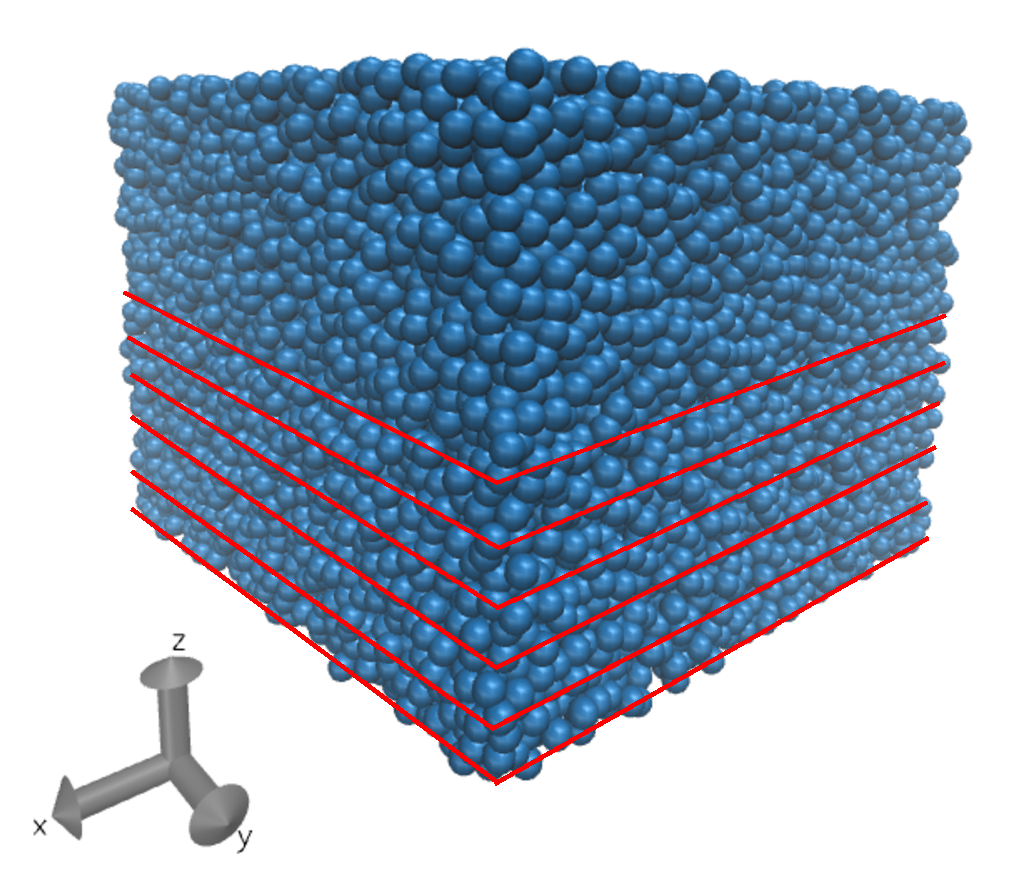
\includegraphics[scale=0.3]{system_nodes_periodic}
    \caption[Periodic box]{A visual representation of the MD simulation with a sketch of the binning used. In red are depicted the nodal planes used.}
    \label{fig:PBCBox}
\end{figure}
We carefully  distinguish between  \textit{nodes} and
\textit{bins}:  nodes are  points  in  the $z$  axis,  while bins  are
segments in this axis.  In 3D, nodes are planes, while bins are slabs.
As it  will become apparent, from  a microscopic point of  view, mass,
momentum, and force  densities are defined at the  nodes, while stress
is  defined  at  the  bins.   Each   bin  is  a  layer  of  dimensions
$L_x,L_y,\Delta z$. 


As CG variables we choose  the set of discrete hydrodynamic
variables,  which are  the  mass density  $\hat{\rho}_\mu(z)$ and  the
momentum  density $\hat{\bf  g}_\mu(z)$  defined at  the nodal  planes
$\mu$   \Note{Realmente la única variable relevante es el momento.}
\begin{align}
\hat{\rho}_\mu(z)&= \sum_i^Nm_i\delta_\mu({\bf r}_i)
% \nonumber\\
% \hat{e}_\mu(z)&= \sum_i^Ne_i\delta_\mu({\bf r}_i)
\nonumber\\
\hat{\bf g}_\mu(z)&= \sum_i^N{\bf p}_i\delta_\mu({\bf r}_i)
%\label{rhogmumic}
\end{align}
where ${\bf r}_i,{\bf p}_i$ are the position and momentum of particle $i$, 
 the discrete Dirac delta function as 
\begin{align}
\delta_\mu({\bf r})&=  \frac{1}{{\cal V}_\mu}\Phi_\mu({\bf r})
\label{delta}
\end{align}
with the volume defined as
\begin{align}
  {\cal V}_\mu&=\int d{\bf r}\Phi_\mu({\bf r}),
\end{align}
and $\Phi_\mu({\bf r})$  is the finite element basis  function, a tent
function centered  at the nodal plane  $\mu$ and that depends  only on
the $z$ component  of ${\bf r}$.  The mass density  at a node receives
information about the  mass of fluid molecule $i$ that  depends on the
distance of this molecule to the  nodal plane $\mu$, and similarly for
the  momentum.   The  microscopic  variables  (\ref{rhogmumic})  give,
essentially, the number  of particles and momentum per  unit volume of
the particles that happen to be ``around'' the nodal plane $\mu$.  The rationale for using this definition has been discussed in Chapter (\ref{Chap:Planar})


Note that the finite  element basis  functions $\Phi_\mu({\bf  r})$  form a
partition of unity, i.e.
\begin{align}
  \sum_\mu\Phi_{\mu=1}^{N_{\rm bin}}({\bf r})=1
\label{PartUnit}
\end{align}
The  partition  of unity  implies  that  if  we compute  the  discrete
integral  (i.e. sum  over bins  times the  volume of  the bin)  of the
discrete hydrodynamic variables we obtain
\begin{align}
  \sum_\mu{\cal V}_\mu\hat{\rho}_\mu(z)&  &&= mN
\nonumber\\
  \sum_\mu{\cal V}_\mu\hat{\bf g}_\mu(z)&=\sum_i^N{\bf p}_i&&= \hat{\bf P}_T(z)
\label{DiscCons}
\end{align}
where we  have introduced the total  mass $mN$ and the  total momentum
$\hat{\bf  P}_T(z)$ of  the  system.  These  are  quantities that  are
conserved under  the Hamiltonian  evolution of the  microscopic state.


In this work we  will only  consider the correlations  of the
component  $\hat{g}^1_\mu$ of  the  momentum density  parallel to  the
bins. These variables are collected into the $N_{\rm bin}$-dimensional
vector           $\hat{g}(z)=\{\hat{g}^1_1(z),\cdots,\hat{g}^1_{N_{\rm
    bin}}(z)\}$ of the $x$ component  of the discrete momentum density
of each of the ${N_{\rm bin}}$ bins in which the periodic box has been
divided.  We  have checked  through MD  simulations that  the coupling
between  this  component  and   the  rest  of  hydrodynamic  variables
(density,  other momentum  components) is  negligible.  Therefore,  we
expect  that a  theory  of  just the  transverse  momentum  is a  good
candidate for  a Markovian theory.  
%Sound perpendicular to  walls that
%requires both the mass density  and the perpendicular component of the
%discrete momentum will be considered elsewhere.

\subsection{The dynamics}
\label{Sec:Trans}
The correlation matrix of the  CG variables $\hat{A}$, assumed to have zero
equilibrium average, is 
\begin{align}
  C(t)&=\llangle \hat{A}(t)\hat{A}^T\rrangle
\end{align}
where the $\llangle\cdots\rrangle$ denotes the equilibrium average and
$T$ is for transpose. 

Mori theory for correlations presented in Sec. (\ref{Sec:Mori}) allows us to obtain the evolution of the matrix of correlations $C(t)$ as
\begin{align}
    \frac{d}{dt}C(t) = -(L+M^*)\cdot C^{-1}(0)\cdot C(t),
\end{align}
where we have use the equations (\ref{AproxC}), (\ref{Lambda}) and the normalized correlation matrix defined as
\begin{align}
  c(t)=C^{-1}(0)\esc C(t)
\end{align}
Note that the reversible matrix $L$ vanishes because it involves an equilibrium average of a function that is even in the momentum variables \Note{Comprobarlo}. Therefore
\begin{align}
    \frac{d}{dt}C(t) = -k_BTM^*\cdot c(t)
    \label{AproxCg}
\end{align}
where, in order to make contact  with known results, we have redefined
the transport  matrix $M^*$  by introducing  a prefactor  $k_BT$ where
$k_B$ is Boltzman's constant and $T$ the equilibrium temperature. 
%As a final
%remark, note that the Markovian equation (\ref{AproxCg}) cannot hold at
%$t=0$, because in that case we get $0=-k_BTM^*$, which is non-sense. Clearly,
%such a Markovian equation can only hold beyond certain time $\tau$, related
%to the neglected memory.

\subsection{The Green-Kubo running integral $M(t)$}
The friction matrix $M^*$ in (\ref{GKCorrected}) is
related to the standard Green-Kubo running integral
\begin{align}
M(t)&=\frac{1}{k_BT}\int_0^{t}dt' \llangle i{\cal L}\hat{g}(t')i{\cal L}\hat{g}^T\rrangle
\label{Mmunu}
\end{align}
that  involves the  time
derivative of the  momentum density which, as shown  in Eq. \Pendiente{(\ref{} Versión disceta)}, is
given by
\begin{align}
  i{\cal L}  \hat{g}_{\mu}(z)&=-\frac{\hat{\sigma}^{13}_{\mu}-\hat{\sigma}^{13}_{\mu-1}}{\Delta z}
\label{iLAcurrentx}
\end{align}
This  is a  discrete expression  of the  momentum balance  equation in
which the time rate of change of the momentum of the node $\mu$ is due
to   the   finite   difference   gradient   of   the   stress   tensor
$\hat{\sigma}^{13}_{\mu}$  of  the  neighbour bins.   The 
microscopic   stress   tensor   of  bin $\mu$ is 

\begin{align}
 \hat{ \boldsymbol{\sigma}}_{\mu}
% &=\hat{\bf K}_\mu+\hat{\boldsymbol{\Pi}}_{\mu}
% \nonumber\\
&=
\frac{1}{{\cal V}_\mu} \left[\sum_i{\bf p}_i{\bf v}_i\chi_\mu({\bf r}_i)
+\frac{1}{2}\sum^{N}_{ij}{\bf r}_{ij}\hat{\bf F}_{ij}z_\mu(i,j)\right]
\label{sbin}
\end{align}
where $\chi_\mu({\bf r})$ is the  characteristic function of bin $\mu$
and $z_{\mu}(i,j)$ is the fraction of the distance between atoms $i,j$
that happens to be within bin $\mu$ (\Pendiente{\ref{} Ref.Versión discreta}).

We may write Eq. (\ref{iLAcurrentx}) in matrix form as
\begin{align}
  i{\cal L}\hat{g}&= -B\esc\hat{\sigma}^{13} =F^T\esc\hat{\sigma}^{13}
\label{iLgMat}
\end{align}
where  $\hat{\sigma}$ is  a  $N_{\rm  bin}$-dimensional column  vector
containing the  discrete stress tensor  of bin  $\mu$ and $B$  is the
backward finite difference matrix.  This matrix is $B=-F^T$, where the
matrix $ F$ is the forward finite difference operator (for PBC)
\begin{align}
 {F}=\frac{1}{\Delta z}\left(
    \begin{array}{rrrrr}
-1&1&0&\cdots&0\\
0&-1&1&\cdots&0\\
\vdots      &&\ddots&&\vdots\\
\\
0&\cdots&0&-1&1 
\\
1&\cdots&0&0&-1 \end{array}
\right)
\label{Dforward}
\end{align}
By using (\ref{iLgMat}) into the Green-Kubo integral matrix $M(t)$ in (\ref{Mmunu})
we have
\begin{align}
  M(t)=F^T\esc\eta(t)\esc F
\label{Mtfef}
\end{align}
where  the  \textit{nonlocal  viscosity  Green-Kubo  matrix}  is  the
running  time integral  of the  correlation  of the  stress tensor  at
different bins,
\begin{align}
  \eta(t) &=\frac{1}{k_BT}\int_0^{t}dt' 
  \llangle \hat{\sigma}^{13}(t')\hat{\sigma}^{13}\rrangle
\label{non-loc}
\end{align}
Note that  for a homogeneous system  (as one with PBC),  the nonlocal
viscosity    matrix   is    translationally    invariant,   this    is
$\eta_{\mu\nu}=\eta(|\mu-\nu|)$.  This kind  of matrices  commute with
the forward differencing matrix
\begin{align}
  F\esc\eta(t)=\eta(t)\esc F
\label{commute}
\end{align}
By using this commutation property 
 in the Green-Kubo
integral (\ref{Mtfef}) we obtain
\begin{align}
  M(t)=-\Delta\esc \eta(t)
\label{MmunuMat}
\end{align}
where we have introduced  the discrete Laplacian matrix (for PBC) as
\begin{align}
\Delta&\equiv  B\esc F
=\frac{1}{\Delta z^2}\left(
    \begin{array}{rrrrr}
-2&1&0&\cdots&1\\
1&-2&1&\cdots&0\\
\vdots      &&\ddots&&\vdots\\
\\
1&\cdots&0&1&-2    \end{array}
\right)
\end{align}

Note that the Green-Kubo integral (\ref{Mmunu}) can also be written
in the form
\begin{align}
    M(t)&= \frac{1}{k_BT} \int_0^t dt'\frac{d}{dt'}\llangle \hat{g}(t') i{\cal L}\hat{g}^T\rrangle
\nonumber\\
&= \frac{1}{k_BT} \llangle \hat{g}(t) i{\cal L}\hat{g}^T\rrangle
=  -\frac{1}{k_BT}\frac{d}{dt}\llangle \hat{g}(t) \hat{g}^T\rrangle=-\frac{1}{k_BT}\frac{d}{dt}C(t)
\label{E1}
\end{align}
Therefore,  Eqs  (\ref{MmunuMat}),(\ref{E1})  lead  to  the  following
\textit{rigorous and exact} result
\begin{align}
\frac{d}{dt}C(t)&= k_BT \Delta\esc \eta(t)
\label{etaExact}
\end{align}
that links the momentum correlation matrix with the stress correlation
matrix.  This  equation shows  that  the  Green-Kubo running  integral
(\ref{non-loc})  for  the viscosity  matrix  $\eta(t)$  cannot have  a
plateau, as it should decay according to the time derivative of $C(t)$
and,  hence, from  (\ref{AproxC})  as the  correlation matrix  $C(t)$
itself.

\subsection{The  friction   matrix  $M^*$  and  the   nonlocal  shear
  viscosity matrix}
By analogy with  (\ref{MmunuMat}), we assume that the  friction matrix $M^*$ in
(\ref{AproxCg}) has the structure
\begin{align}
  M^*=-\Delta\esc \eta^*
\end{align}
for a  certain  matrix  $\eta^*$  referred to  as  the  nonlocal  shear
viscosity  matrix.  The Markovian  dynamics  (\ref{AproxCg})
becomes
\begin{align}
\frac{d}{dt}C(t)&=  k_BT\Delta\esc \eta^*\esc c(t)
\label{AproxCg1}
\end{align}
We  would like  to  obtain  the matrix  $\eta^*$  from the  Green-Kubo
running  integral   (\ref{non-loc})  for  $\eta(t)$.    Comparison  of
(\ref{AproxCg1}) and (\ref{etaExact}) gives
\begin{align}
 \Delta\esc \eta(t) &=\Delta\esc \eta^*\esc c(t)
\label{etaExact1}
\end{align}
If   the   two   matrices    $\Delta,c(t)$   were   invertible,   then
(\ref{AproxCg1}) would  allow to obtain $\eta^*$  from the correlation
of  the  momentum  density,  while Eq.  (\ref{etaExact1})  would  give
$\eta^*$  from the  correlation of  the  stress. Both  routes are,  of
course, mathematically equivalent.  However, both the Laplacian matrix
$\Delta$  and  the  normalized   correlation  matrix  $c(t)$  are  not
invertible.  The reason is that the normalized ``constant'' vector
\begin{align}
  v&=\frac{1}{\sqrt{M}}(1,1,\cdots,1)
\end{align}
is the unique eigenvector of null eigenvalue of the Laplacian operator
with periodic boundary conditions, $\Delta  \cdot v=0$. This vector is
also  eigenvector  of  null   eigenvalue  of  the  correlation  matrix
$C(t)\esc v=0$  due to total momentum  conservation in PBC. 
%Que no tengan un autovalor nulo es condición necesaria para que una matriz sea invertible.
%These two  matrices are
%not invertible, although they are so in the subspace normal to $v$. It is 
%much easier to deal with this issue in Fourier space.
In the next section we take advantage of the periodicity and the translational invariance of the system in order to deal with that issue in Fourier space. 

\subsection{Fourier space}
Consider the unitary matrix with elements
\begin{align}
E_{\mu\nu}=\frac{1}{\sqrt{N_{\rm bin}}}\exp\left\{i\frac{2\pi}{N_{\rm bin}}\mu\nu\right\}
\end{align} 
This matrix has the following inverse
\begin{align}
E^{-1}_{\mu\nu}=\frac{1}{\sqrt{N_{\rm bin}}}\exp\left\{-i\frac{2\pi}{N_{\rm bin}}\mu\nu\right\}
\end{align} 
The indices  are assumed  to run  in the  range $\mu=0,1,\cdots,N_{\rm
  bin}-1$.  
We define the Fourier transform $\tilde{A}$ of a matrix $A$ as
\begin{align}
    \tilde{A}&=E^{-1}\esc A\esc{E}
 \end{align}
with the inverse relation 
 \begin{align}
     A&=E\esc  \tilde{A}\esc{E}^{-1}
\label{FT}
\end{align}
The discrete Laplace operator diagonalizes in Fourier space, this is
\begin{align}
  E^{-1}  \esc {\Delta} \esc E= \tilde{\Delta}
\label{EDE}
\end{align}
where $\tilde{\Delta}$ is a diagonal matrix whose diagonal  elements are
\begin{align}
\tilde{\Delta}_{\mu\mu}&=-\frac{2}{\Delta z^2}
\left(1-\cos\left( \frac{2\pi \mu}{N_{\rm bin}}\right)\right)\le0  
\label{Dmumu}
\end{align}
This is the  spectrum of the discrete Laplace  operator $\Delta$. 


The matrix $E$ diagonalizes any traslation invariant and periodic
matrix    $A_{\mu\nu}$    satisfying    $A_{\mu\nu}=a(|\mu-\nu|)$    and
$a(\mu)=a(N_{\rm bin}-1-\mu)$ as it is easily seen
\begin{align}
&\left[  E^{-1}\esc A\esc E\right]_{\mu\nu}
\nonumber\\
&=
\frac{1}{N_{\rm bin}}\sum_{\mu'=0}^{N_{\rm bin}-1}\sum_{\nu'=0}^{N_{\rm bin}-1} e^{-i\frac{2\pi}{N_{\rm bin}}\mu\mu'}a(|\mu'-\nu'|)
e^{i\frac{2\pi}{N_{\rm bin}}\nu'\nu}
 \nonumber\\
&=\frac{1}{N_{\rm bin}}\delta_{\mu\nu}\underbrace{\sum_{\sigma=0}^{N_{\rm bin}-1}a(\sigma)e^{i\frac{2\pi}{N_{\rm bin}}\sigma\nu}}_{\tilde{a}(\nu)}
\end{align}

Because  the  matrix  $C(t)$  is periodic  traslation  invariant,  the
Fourier     transform     is     a    diagonal     periodic     matrix
$\tilde{C}_{\mu\nu}(t)=\delta_{\mu\nu}\tilde{C}_{\mu\mu}(t)$.
The two equations (\ref{AproxCg1}),(\ref{etaExact1}) become in Fourier space
\begin{align}
  \frac{d}{dt}\tilde{C}(t)&=  k_BT\tilde{\Delta}\esc \tilde{\eta}^*\esc \tilde{c}(t)
\nonumber\\
 \tilde{\Delta}\esc \tilde{\eta}(t) &=\tilde{\Delta}\esc \tilde{\eta}^*\esc \tilde{c}(t)
\label{Fou1}
\end{align}
All matrices  appearing in  these equations are  diagonal.  Therefore,
except  for $\mu=0$,  where $\tilde{c}_{00}=0$  due to  total momentum
conservation,  we  may  infer  the  diagonal  elements  of  the  shear
viscosity matrix in Fourier space  $\tilde{\eta}^*$ from either any of
these two equations
\begin{align}
  \tilde{\eta}^*_{\mu\mu}&= \frac{1}{ k_BT\tilde{\Delta}_{\mu\mu}  \tilde{c}_{\mu\mu}(t)}\frac{d}{dt}\tilde{C}_{\mu\nu}(t)
\nonumber\\
\tilde{\eta}_{\mu\mu}^*&=\frac{\tilde{\eta}_{\mu\mu}(t) }{\tilde{c}_{\mu\mu}(t)}
\label{FouFin}
\end{align}
These two expressions are mathematically  equivalent but they allow to
obtain   the    nonlocal   shear    viscosity   in    Fourier   space
$\tilde{\eta}_{\mu\mu}^*$ either  from the correlation of  momemtum or
from the  correlation of stress.   The existence  of a plateau  in the
time-dependent  functions of  the  right hand  side in  (\ref{FouFin})
constitute both, a validation of  the Markovian assumption, as well as
a way to computate the nonlocal shear viscosity.

If we wish  to recover the nonlocal shear viscosity  in real space we
need   to  know   all   their  eigenvalues.    However,  the   element
$\tilde{\eta}_{00}$  cannot be  computed  from (\ref{FouFin})  because
$\tilde{c}_{00}=0$.  Note that this value  can be obtained directly by
recognizing that
\begin{align}
    \tilde{\eta}_{00}(t)&=E_{0\mu}^{-1}\cdot\eta_{\mu\nu}(t)\cdot E_{\nu 0}=\frac{1}{N_{\rm bin}}
\sum_{\mu\nu}\eta_{\mu\nu}(t)
\label{eta00}
\end{align}
From
(\ref{sbin}) and the fact that $\chi_\mu({\bf r}),z_{\mu}(i,j)$ form a partition of unity, we have
that the total stress is the arithmetic average of the stress in each bin is given by
\begin{align}
\hat{\sigma}_T^{13}=\frac{1}{N_{\rm bin}}\sum_\mu\hat{\sigma}_\mu^{13}
\label{TotStress2}
\end{align}
where the  total stress $\hat\sigma_T^{13}$ is defined  in the usual way
\begin{align}
\hat{\sigma}_T^{13}&=\frac{1}{V_T}\left[\sum_{i}{\bf p}^1_i{\bf v}^3_i
+\frac{1}{2}\sum_{ij}{\bf r}^1_{ij}\hat{\bf F}^3_{ij}\right]
\label{TotStress}
\end{align}
and $V_T$ is the total volume of the system. 

By using (\ref{non-loc}) in (\ref{eta00}) we obtain
\begin{align}
    \tilde{\eta}_{00}(t)&=\frac{1}{N_{\rm bin}}\frac{1}{k_BT}\int_0^tdt'\llangle \sum_{\mu}\hat{\sigma}^{13}_{\mu}(t')\sum_{\nu}\hat{\sigma}^{13}_{\nu}\rrangle
\end{align}
Using the Eq. (\ref{TotStress2})
\begin{align}
    \tilde{\eta}_{00}(t)&=\frac{N_{\rm bin}}{k_BT}\int_0^tdt'\llangle \hat{\sigma}^{13}_T(t')\hat{\sigma}^{13}_T\rrangle
\end{align}
Introducing the \textit{local}  shear viscosity given by the standard Green-Kubo
integral
\begin{align}
  \eta_0(t) &\equiv \frac{V_T}{k_BT}\int_0^t dt'\llangle \hat{\sigma}_T^{13}(t')\hat{\sigma}_T^{13}
\rrangle
\label{etat}
\end{align}
we finally reach 
\begin{align}
    \tilde{\eta}_{00}(t)=\frac{N_{\rm bin}}{V_T}\eta_0(t)
\end{align}
Therefore, the eigenvalue $\tilde{\eta}_{00}(t)$ can be computed independently from
the local shear viscosity.

\subsection{The nonlocal kinematic viscosity matrix}
It is convenient to introduce the nonlocal kinematic viscosity matrix
$\nu^*$ as  the nonlocal shear  viscosity matrix $\eta^*$  divided by
some ``mass density''. As we will see, the notion of locality in space
is best addressed with the kinematic  viscosity and that is the reason
of introducing it here. In  a discrete setting, the connection between
the  discrete momentum  and  the discrete  velocity  is slightly  more
involved than  in the continuum  for which  one has the  simple result
${\bf g}({\bf  r})=\rho({\bf r}){\bf  v}({\bf r})$.  In  the discrete,
the proportionality  between velocity and  momentum is through  a mass
density \textit{matrix} \cite{3}.  Let us see the details.

\Pendiente{As  shown  in Appendix  \ref{Ap:Cov},  the  covariance $C(0)$  of  the
discrete momentum density in PBC is given by
\begin{align}
C_{\mu\nu}(0)&= \frac{k_BT}{{\cal V}_\mu} \rho_{\mu\nu}
\label{gg}
\end{align}
where we have introduced the mass density matrix $\rho_{\mu\nu}$ as
\begin{align}
  \rho_{\mu\nu}&\equiv  m{\cal V}_\mu n \left[ M^\delta_{\mu\nu}-
\frac{1}{n N}  \llangle \hat{n}_\mu\hat{n}_\nu\rrangle\right]
\label{MassMat}
\end{align}
where  $\hat{n}_\mu=\hat{\rho}_\mu/m$ is  the number  density  of node $\mu$ and $n=N/V$  is the  average
number density.  The
matrix $M^\delta_{\mu\nu}$ is
\begin{align}
  M^\delta_{\mu\nu}&=\int d{\bf r}\delta_\mu({\bf r})\delta_\nu({\bf r}) 
\end{align}
For a system  with regular bins with constant volume  ${\cal V}$ each,
this matrix takes the form
\begin{align}
{M}^\delta&=\frac{1}{6{\cal V}}
\left(\begin{array}{cccccc}
4&1&0&\cdots &0&1\\
1&4&1&\cdots &0&0\\
\vdots&&&\ddots&&\vdots\\
0&0&0&\cdots &4&1\\
1&0&0&\cdots&1&4
\end{array}\right)
\end{align}
The last  term in (\ref{MassMat}) scales  as the inverse of  the total
number  $N$ of  particles and  it is  negligible in  the thermodynamic
limit.  However, we  should keep it as it  has observable consequences
in  our simulations.   In fact,  this  term is  responsible for  total
momentum conservation (\ref{DiscCons}), this is
\begin{align}
  \sum_\mu{\cal V}_\mu\llangle \hat{g}_\mu\hat{g}_\nu\rrangle &=0
\end{align}
as   it   should,   because    the   total   momentum   $\sum_\mu{\cal
  V}_\mu\hat{g}_\mu$ vanishes  in the  center of mass  reference frame
that we take.
} %Fin pendiente


By using the explicit form (\ref{gg}) of the covariance matrix, we may
express Eq. (\ref{AproxCg1}) in the form
\begin{align}
\frac{d}{dt}C(t)= \Delta\esc \nu^*\esc C(t)
\label{SDECpi}
\end{align}
where we  have introduced  the nonlocal  \textit{kinematic} viscosity
matrix through the matrix
\begin{align}
\nu^*&\equiv  \eta^*\esc{\cal V}\esc \rho^{-1}
\label{nustar}
\end{align}
where ${\cal  V}$ is a diagonal  matrix that contains in  the diagonal
the volume ${\cal  V}_\mu$ of the bins.   In Fourier space Eq. (\ref{nustar})
takes the diagonal form
\begin{align}
  \tilde{\nu}_\mu^*&=  \frac{{\cal V}_\mu \tilde{\eta}_\mu^*}{\tilde{\rho}_\mu}
\end{align}
We now show why we refer to the matrix $\eta^*$ as the nonlocal shear
viscosity  and  to  the  matrix $\nu^*$  as  the  nonlocal  kinematic
viscosity.   According   to  Mori  theory,  which   encompass  Onsager
regression  hypothesis, the  evolution  of the  average  value of  the
discrete momentum should evolve according to a vector equation analogous to
(\ref{SDECpi}) for the correlation matrix
\begin{align}
  \frac{d}{dt}g(t)&={\cal V}\esc \Delta\esc\eta^*\esc v(t)
%   \frac{d}{dt}g(t)&=\Delta\esc
% \eta^*\esc k_BTC^{-1}(0)\esc g(t)
\label{dgDnug}
\end{align}
where we have defined the discrete velocity field $v$ according to

\begin{align}
  v_\mu&\equiv\sum_\nu \rho_{\mu\nu}^{-1}g_\nu
\label{vel}
\end{align}
The matrix  $\rho_{\mu\nu}$ defined in (\ref{MassMat})  has dimensions
of a mass density and it  is fairly diagonal.  Its inverse $\rho^{-1}$
is concentrated on the diagonal (in fact, it decays exponentially fast
as we move out from the diagonal).  Because of this, we may interprete
$v_\mu$ defined in (\ref{vel}) as a velocity that contains information
about   the   discretization   method   used.    The components of
Eq. (\ref{dgDnug}) are
\begin{align}
  \frac{d}{dt}{g}_\mu(t)&=
-\sum_\nu{\cal V}_\nu 
\frac{\left[
\eta^*_{\mu+1\nu}-2\eta^*_{\mu\nu}+\eta^*_{\mu-1\nu}\right]}{\Delta z^2}{v}_\nu^1(t)
\end{align}
where we have used the translation invariance of the viscosity matrix.
By a suitably rellabeling  of indices we have
\begin{align}
  \frac{d}{dt}{g}_\mu(t)&=\sum_\nu{\cal V}_\nu \eta^*_{\mu\nu}
\frac{\left[{v}_{\nu+1}^1-2{v}_{\nu}^1+{v}_{\nu-1}^1\right]}{\Delta z^2}
\label{SDELap0} 
\end{align}

Eq. (\ref{SDELap0}) looks    like    a   discretization    of    the    following
integro-differential  equation
\begin{align}
  \frac{d}{dt} g^1(z)&=\int dz'{\eta}^*(z-z')\partial^2_{z'} v^1(z')
\label{congx}
\end{align}
This is  a nonlocal generalization  of the diffusion equation  of the
continuum transverse  momentum,
\begin{align}
  \partial_t g^1(z)&=\nu^*_0\partial^2_{z}g^1(z')
\label{congx3}
\end{align}
Eq.   (\ref{congx3})   is  obtained  from  (\ref{congx})   by  setting
$\eta^*(z-z')=\eta^*_0\delta(z-z')$,   where   the   local   kinematic
viscosity is  $\nu^*_0=\eta^*_0/\rho$.  Therefore, it is  justified to
refer to the matrix $\eta^*_{\mu\nu}$ introduced in (\ref{non-loc}) as
the  nonlocal shear  viscosity matrix  and to  $v_\mu$ introduced  in
(\ref{vel}) as the velocity.


\subsection{The local in time prediction}
By using (\ref{EDE})  and (\ref{Dmumu}), the Fourier  transform of the
equation of motion (\ref{SDECpi}) is then
\begin{align}
  \frac{d\tilde{C}_\mu}{dt}(t)&=-\frac{1}{\tau_\mu}\tilde{C}_\mu(t)  
\label{SDECpiDiag}
\end{align}
where the correlation time is given by 
\begin{align}
 \frac{1}{\tau_\mu}&\equiv \frac{2}{\Delta z^2}
\left(1-\cos\left( \frac{2\pi \mu}{N_{\rm bin}}\right)\right)
\tilde{\nu}_\mu^*
\label{taumu}
\end{align}
The  solution of  Eq.  (\ref{SDECpiDiag})  with ``initial  condition''
$\tilde{C}_\mu(\tau)$ at time $\tau$ is the exponential function
\begin{align}
  \tilde{C}_\mu(t)&=\exp\left\{-\frac{t-\tau}{\tau_\mu}\right\}  \tilde{C}_\mu(\tau)
\label{solexp}
\end{align}
The eigenvalues must be decay in an exponential way if the Markovian aproximation is correct. 
The displacement of the initial condition to the time $\tau$ is due to
the fact that  we know that the exponential behaviour  cannot start at
$t=0$  where   the  Markovian  equation  (\ref{AproxC})   and,  hence
(\ref{SDECpiDiag}), cannot hold strictly.

In real space, the correlation matrix is given by Eq. (\ref{SDECpi})
\begin{align}
  C(t)&=\exp\left\{\Delta\esc \nu^* (t-\tau) \right\}C(\tau)
\label{Cmunut}
\end{align}
where the exponential matrix takes the form
\begin{align}
\left[\exp\left\{\Delta\esc \nu^* t \right\}\right]_{\mu\nu}
&=\frac{1}{N_{\rm bin}}\sum_{\mu'}\exp\left\{i\frac{2\pi}{N_{\rm bin}}(\mu-\nu)\mu'\right\}
\nonumber\\
&\times
\exp\left\{-\frac{t}{\tau_{\mu'}}\right\}
\end{align}
In summary, the prediction of the correlation matrix in Fourier space
is given  by single exponentials, while  in real space is  given by a
linear combination of  single exponentials. As we will  see, the later
will give rise to quasi-algebraic decay of correlations.

\subsection{The local in space prediction}
The   discrete   version   of  the   local   continuum   hydrodynamics
Eq. (\ref{congx3}) is simply
\begin{align}
  \frac{d}{dt}{g}_\mu(t)=&\nu_0\Delta_{\mu\nu}{g}_\nu(t)
\label{gloc}
\end{align}
By comparing  this discrete equation  in the local  approximation with
the nonlocal  discrete equation  (\ref{dgDnug}) we conclude  that the
local approximation of the nonlocal viscosity matrix $\nu^*$ becomes a
diagonal matrix of the form
\begin{align}
\nu_{\mu\mu'}^*&\simeq \nu_0 \delta_{\mu\mu'}
\end{align}
where the local kinematic viscosity is given by
\begin{align}
\nu_0&\equiv \sum_{\mu'}\nu_{\mu\mu'}^* \quad \quad \quad\forall \mu
\label{nu0}
\end{align}
In the  local approximation, the differential  equation (\ref{SDECpi})
for the correlation matrix becomes
\begin{align}
  \frac{d}{dt}{C}(t)=&\nu_0{\Delta}\esc { C}(t)
\label{LocalEq}
\end{align}
The Fourier transform of the local Eq. (\ref{LocalEq}) is identical to
(\ref{SDECpiDiag})  but  with  a  constant  value  for  the  kinematic
viscosity in (\ref{taumu})
\begin{align}
\tilde{\nu}^*_\mu&= \nu_0
\label{numunu0}
\end{align}
for all $\mu$. Therefore, the  local hydrodynamic prediction says that
the Fourier kinetic viscosity  coefficients $\tilde{\nu}_\mu$ take the
constant value $\nu_0$ given in (\ref{nu0}).
In the local approximation, the relaxation time (\ref{taumu}) is given by 
\begin{align}
 \frac{1}{\tau^{\rm loc}_\mu}&=\frac{2}{\Delta z^2}
\left(1-\cos\left( \frac{2\pi \mu}{N_{\rm bin}}\right)\right)
\nu_0
\label{taumuloc}
\end{align}

%\subsection{Conclusions of the theory}
%The  two main  quantities of  concern  are the  correlation matrix  of
%discrete momentum  $C(t)$ and the  correlation matrix of  the discrete
%stress  that appears  in  the Green-Kubo  running integral  $\eta(t)$.
%These two  matrices can be measured  from MD simulations. In  order to
%test the locality in time, we use the simple prediction (\ref{solexp})
%for the  eigenvalues of the correlation  matrix. In order to  test the
%nonlocality  in space,  from Eq.   (\ref{FouFin}) we  will infer  the
%nonlocal shear viscosity matrix  $\tilde{\eta}^*$ and from the Fourier
%transform   of  (\ref{nustar})   the  nonlocal   kinematic  viscosity
%$\tilde{\nu}^*$. The local  approximation in space will be  good if we
%can approximate  $\tilde{\nu}^*$ as in (\ref{numunu0}).   Once we have
%measured  $\Lambda^*$  or  equivalently  $\eta^*$ or  $\nu^*$  we  can
%compare  the  prediction  (\ref{Cmunut})  from Mori  theory  with  the
%correlation matrix measured in the simulation.


\section{MD simulations}
\label{Sec:SimPBC}
In Sec. (\ref{Sec:MoriPBC}) we saw that the  two main  quantities of  concern  are the  correlation matrix  of
discrete momentum  $C(t)$ and the  correlation matrix of  the discrete
stress  that appears  in  the Green-Kubo  running integral  $\eta(t)$.
These two  matrices can be measured  from MD simulations. In  order to
test the locality in time, we use the simple prediction (\ref{solexp})
for the  eigenvalues of the correlation  matrix. In order to  test the
nonlocality  in space,  from Eq.   (\ref{FouFin}) we  will infer  the
nonlocal shear viscosity matrix  $\tilde{\eta}^*$ and from the Fourier
transform   of  (\ref{nustar})   the  nonlocal   kinematic  viscosity
$\tilde{\nu}^*$. The local  approximation in space will be  good if we
can approximate  $\tilde{\nu}^*$ as in (\ref{numunu0}).   Once we have
measured  $\Lambda^*$  or  equivalently  $\eta^*$ or  $\nu^*$  we  can
compare  the  prediction  (\ref{Cmunut})  from Mori  theory  with  the
correlation matrix measured in the simulation.

The objective of this section is to present the simulations we made to measure the
momentum  correlation  matrix  $C(t)$  and  the  Green-Kubo  nonlocal
viscosity $\eta(t)$.   From these primary quantities,  we obtain their
Fourier transforms  $\tilde{C}(t),\tilde{\eta}(t)$ which  are diagonal
matrices  due to  traslation invariance.  

\subsection{Simulation set up}
\label{Sec:SimSetUpPBC}
Interactions between equal particles has been simulated in PBC with the open source code LAMMPS \cite{Plimpton1995}. The interaction between particles is describeb by a truncated Lennard-Jones (LJ) potential,
\begin{align}
  V_{ij}(r_{ij}) = \left\lbrace
  \begin{array}{ll}
    4\epsilon_{ij}\left[\left(\frac{\sigma_{ij}}{r_{ij}}\right)^{12}-\left(\frac{\sigma_{ij}}{r_{ij}}\right)^6\right] & \textup{if } r_{ij}\leq r_c \\
    0 & \textup{if } r_{ij}>r_c
  \end{array}
  \right.
  \label{LJ}
\end{align}
where $r_{ij}$ is the distance between particles $i$ and $j$, $\epsilon_{ij}$ is the depth of the potential well, $\sigma_{ij}$ is the distance at which $V_{ij}$ is zero, and $r_c$ is the cutoff radius (taken equal to $2.5\sigma_{ij}$). The parameters $\epsilon_{ij}$ and $\sigma_{ij}$ take the value 1. 

In Fig. \ref{fig:system_nodes_periodic} a snapshot of the simulation is showed.
The box  size is $40\times40\times30$, the  number of particles with mass $m=1$
is $N=28749$, and the time step is $0.002$ in reduced units.  After an
equilibration  of  $10^5$ timesteps  with  a  Langevin thermostate  to
produce a microstate typical  from a thermodynamic point corresponding
to $T=2,\rho=0.6$ in  reduced units, the system is  evolved under NVE
microcanonical conditions for a  further $10^5$ timesteps.  After this
equilibration  phase,  production  runs   of  $15\cdot 10^5$  time  steps  are
launched.   The $z$  axis is  binned  in $60$  bins on  which the  $x$
component of the momentum density is recorded.  The
width of the  bin is $\Delta z=0.5\sigma$ which is  subatomic.  In the
presence of walls,  such a bin allows to resolve  the density layering.  A total of $60\times  60$ correlations corresponding to the
elements of  the correlation matrix  are computed in  each simulation.
The correlations are computed with the LAMMPS command {\it fix ave/correlate}. During $7.5\cdot 10^5$ time steps the $x$ component of the momentum density is recorded every $2$ time steps. These values are used to obtain the correlations with a support of $15\cdot10^4$ time steps. %LAMMPS 7500 puntos curva de correlación separados por 2*dt-> soporte de 15000 (i.e. t=30)
After $7.5\cdot 10^5$ steps the correlations are averaged with the previous one. 
In  order to  increase  statistics,  we 
exploit   the   traslation   invariance   of   the
system.  Although computing  all the  correlation matrix  elements may
seem  unnecessary,  we will  use  the  same methodology  for  confined
fluids. In  this later  case, traslation invariance  is broken  and we
need to consider the full correlation matrix.

\subsection{The correlation matrix $C(t)$}

In  Fig. \ref{fig:Ct-matrix-PBC} we  plot the  correlation  matrix of  the
transverse     momentum      $C_{\mu\nu}(t)=\llangle     g_{\mu}(t)\
g_\nu\rrangle$ at  the time  $t=2$ and $t=0.6$.  This  matrix is  periodic and
traslation invariant.  Therefore, statistical errors have been further
reduced by averaging this matrix ``along diagonals''.  In addition, we
have taken advantadge of the  analytical calculation of the covariance
$\llangle g_{\mu} g_\nu\rrangle$ in the Appendix \ref{Ap:Cov} in a
manner that we describe below.

\begin{figure}[h!]
\centering
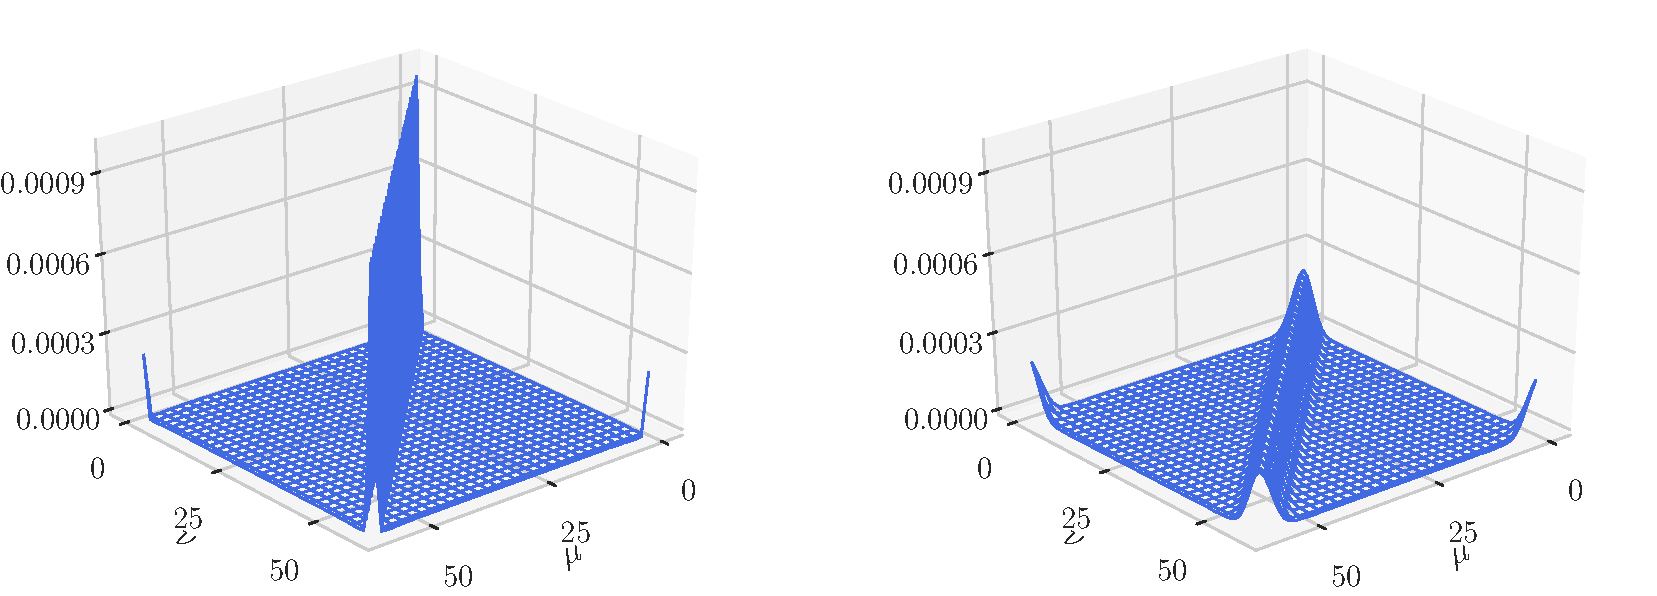
\includegraphics[scale=0.4]{Ct-matrix-PBC}
\caption[Correlation matrix $C(t)$ at $t=0$ and $t=0.6$ for PBC system.]{The   correlation    matrix   $C_{\mu\nu}(t)=\llangle
g_{\mu}(t)  g_\nu\rrangle$ for  $t=0$ (left) and $t=0.6$ (right).}
\label{fig:Ct-matrix-PBC}
\end{figure}

In  Fig.    \ref{fig:Ct-mu30nu-PBC}  the   correlations  $\llangle
g_{\mu}(t)  g_\nu\rrangle$ for  $\mu=30$ and  different values  of
$\nu$ at $t=0$ (blue), $t=0.2$ (orange), $t=0.4$ (purple) and $t= 0.6$ (green) is shown.  This is the row 30 of the matrix plotted
in Fig. \ref{fig:Ct-matrix-PBC}.  We  observe a diffusive
behaviour over  a negative  background.  The  origin of  this negative
global  correlation for  nodes that  are far  appart is  due to  total
momentum conservation in PBC.  If a bin has  a positive momentum, the rest of
bins should  have an  overall negative  value in  order for  the total
momentum to  be zero. In order  to improve the statistical  quality of
the matrix  $C(t)$ we have  used the analytical value  (\ref{Cneg}) of
the  background,  as  provided  by the  analytic  calculation  of  the
covariance in the Appendix \ref{Ap:Cov}.

\begin{figure}[h!]
\centering
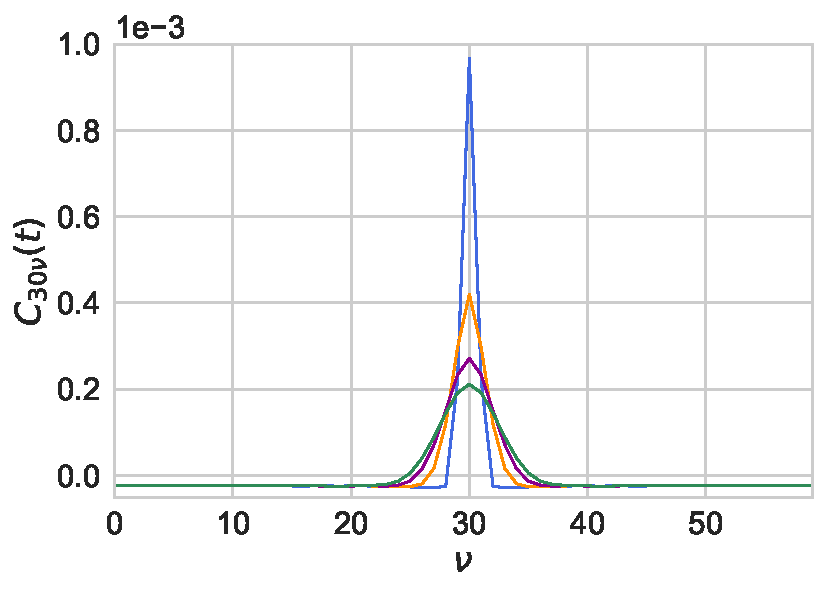
\includegraphics[scale=0.45]{Ct-mu30nu-PBC}
\caption[$C_{30\nu}(t)$ for PBC system.]{$C_{\mu\nu}(t)=\llangle  g_{\mu}(t) g_\nu\rrangle$  for $\nu=30$
 as a  function of node index  $\nu$ and for times $t=0, 0.2, 0.4, 0.6$ in descending order.}
 \label{fig:Ct-mu30nu-PBC} 
\end{figure}

The autocorrelation $\llangle  g_{\mu}(t) g_\mu\rrangle$ (which is
the same for  all $\mu$) is shown in  Fig.  \ref{fig:Autocorrelation-PBC}
as a function of time in both  linear and log scales.  Also shown is a
function $\propto  t^{-1/2}$.  The observed decay  does not correspond
to this algebraic decay.  As discussed in Appendix \ref{Ap:Cont}, only
in both,  the continuum and  thermodynamic limits, we expect  the long
time  tail   $\propto  t^{-1/2}$  behaviour  predicted   by  continuum
hydrodynamics.

\begin{figure}[h!]
\centering
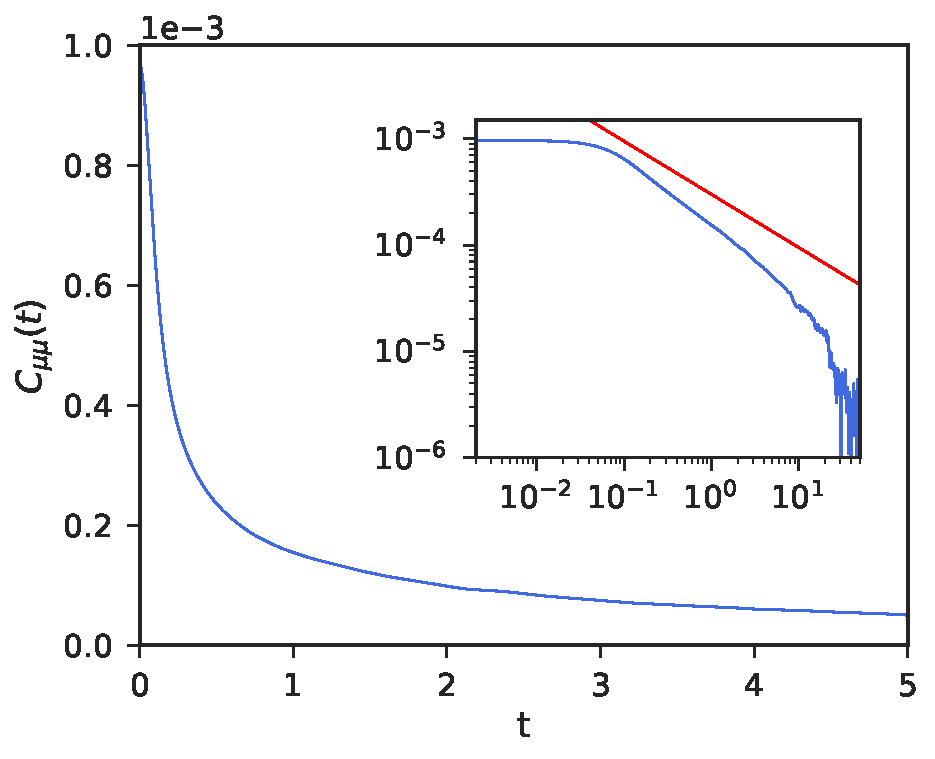
\includegraphics[scale=0.45]{Ct-mu30nu30-PBC}
\caption[Autocorrelation for PBC system.]{The autocorrelation
  $\llangle g_{\mu}(t) g_\mu\rrangle$ (for  any $\mu$)
  . The correlation  decays very
slowly, in an  apparent algebraic way as can be  seen in logscale in the inset.}
  \label{fig:Autocorrelation-PBC}
\end{figure}


\begin{figure}[h!]
  \centering
  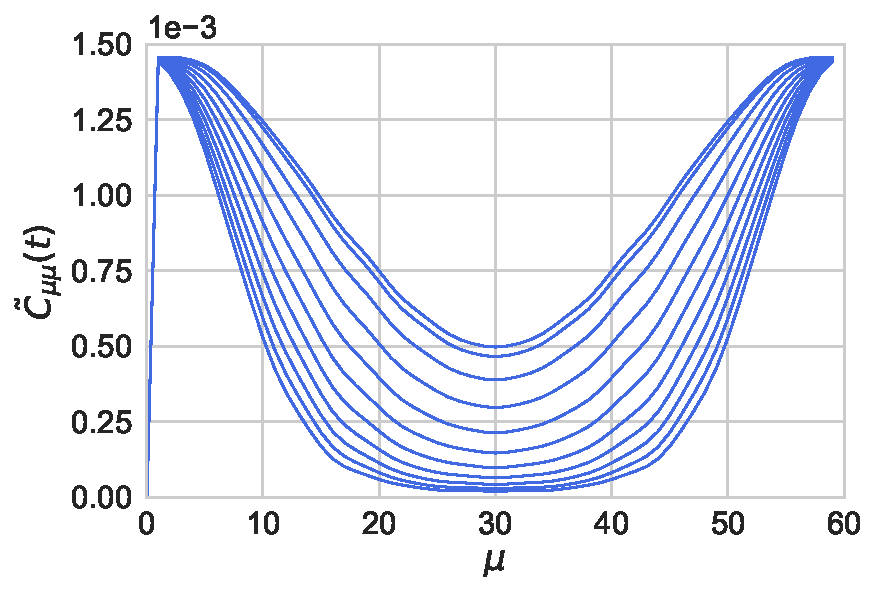
\includegraphics[scale=0.45]{CtFourier-PBC}
  \caption[Diagonal $\tilde{C}_{\mu\nu}(t)$ for PBC]{The diagonal $\tilde{C}_{\mu\mu}(t)$ of the Fourier transform
  of the correlation  matrix $C(t)$ for different values  of the time.
In      descending     order      the     plotted      times go from $t=0.10$ to $t=0.20$ in intervals of $0.02$. }
\label{fig:CtFourier-PBC}
\end{figure}

\begin{figure}[h!]
  \centering
  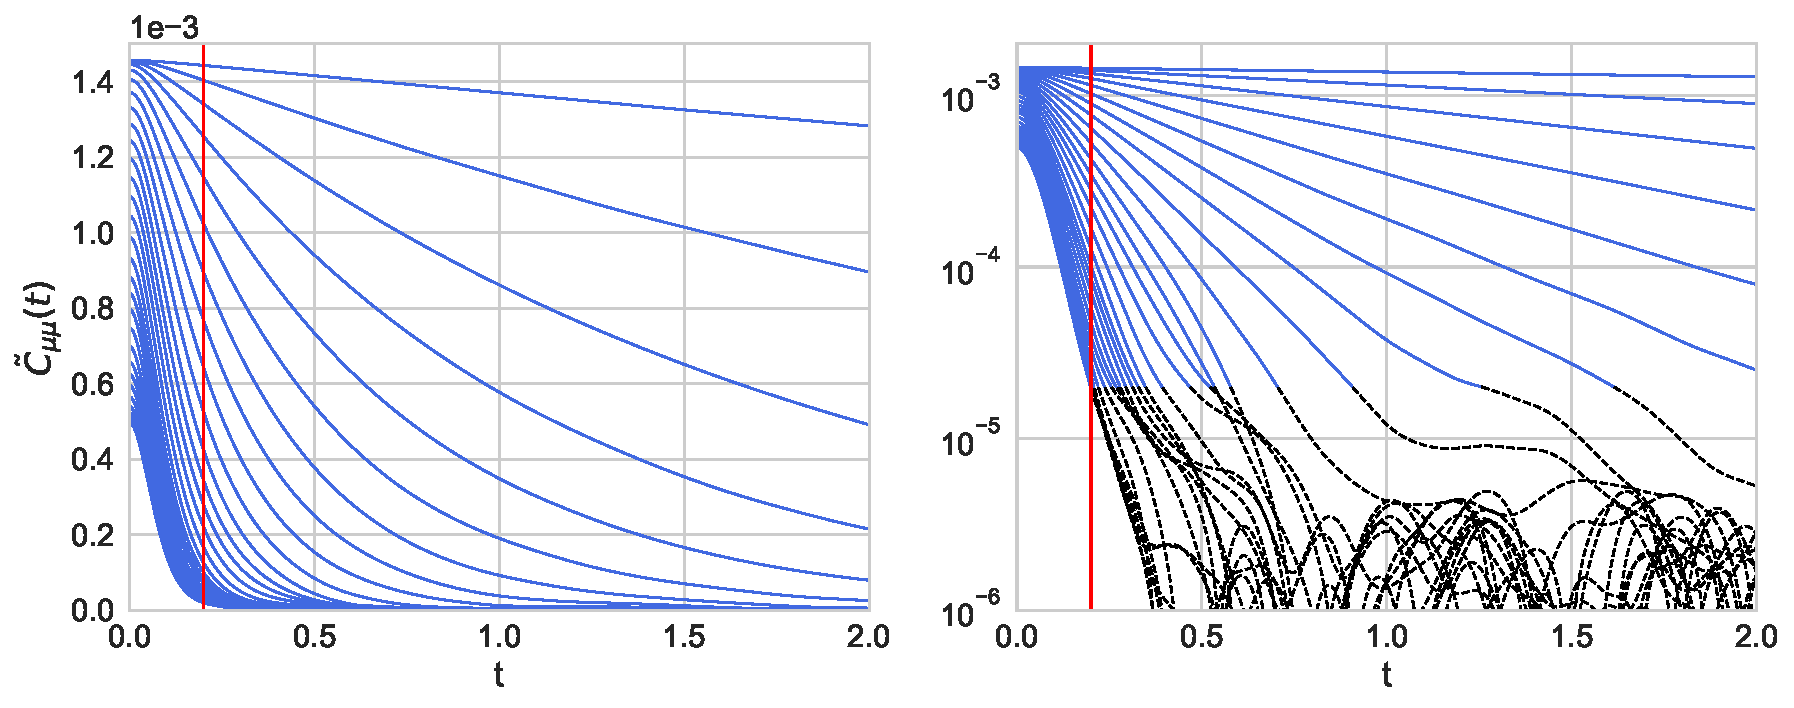
\includegraphics[scale=0.45]{CtFourier-PBC-exp}
  \caption[Evolution of different eigenvalues $\tilde{C}_{\mu\nu}(t)$ for PBC]{
  The  evolution of  the different
  eigenvalues  $\tilde{C}_{\mu\mu}(t)$ of  the  correlation matrix  of
  momentum  as  a  function  of   time  in  a  lin-lin  plot  (left)
  and   log-lin   plot
  (right). Also  plotted are  a vertical line  at $t=\tau=0.2$  and a
  horizontal  line  at  the   value  $2\times10^{-5}$,  signaling  the
  threshold below which statistical errors give spurious results. }
\label{fig:CtFourier-PBC-exp}
\end{figure}

The Fourier transform $\tilde{C}(t)$  of the correlation matrix $C(t)$
is a diagonal matrix.  The diagonal $\tilde{C}_{\mu\mu}(t)$ is plotted
in Fig.   \ref{fig:CtFourier-PBC} as a function of the mode
$\mu$      for      different       values      of      the      time,
from $t=0.10$ to $t=0.20$ in intervals of $0.02$ in  descending   order.   Note that the  mode
$\mu=0$ gives a vanishing value  because of momentum conservation. At the largest times plotted,
the  value  of  the  diagonal  correlation  matrix  in  Fourier  space
$\tilde{C}_\mu(t)$ goes to  zero for modes with  values near $\mu=30$,
implying the  amplification of the  statistical errors in  the inverse
matrix in that  region.  In Fig.  \ref{fig:CtFourier-PBC-exp}  left panel we
plot the  eigenvalues $\tilde{C}_{\mu\mu}(t)$  as a function  of time.
Observe  that after  a time  around  $\tau=0.2$ (red line) the  decay in  log-lin
(right  panel) is  approximately  linear,  suggesting an  exponential
decay. Also we have represented in black and dashed lines the values of the eigenvalues $\tilde{C}_{\mu\nu}$ which statistical errors give spurious results. 


\subsection{Validation of the Markov property}
\label{Sec:ValidateMarkovPBC}
When the  Markov equation (\ref{AproxC})  is valid, we have  that the
eigenvalues of  the correlation matrix decay  exponentially, according
to the prediction (\ref{SDECpiDiag}).  In order to better discriminate
the exponential behaviour we introduce the time-dependent matrix
\begin{align}
\Lambda(t)\equiv-    \frac{dC}{dt}(t)\esc C^{-1}(t)
\label{AproxCtau}
\end{align}
that according  to the Markov equation  (\ref{AproxC}), should evolve
towards a constant time  independent matrix $ \Lambda(t)\to \Lambda^*$
after   certain  time.   In  Fourier   space  all   matrices  in   Eq.
(\ref{AproxCtau}) are diagonal and, therefore
\begin{align}
\tilde{\Lambda}_{\mu\mu}(t)\equiv -    \frac{1}{\tilde{C}_{\mu\mu}(t)}\frac{d\tilde{C}_{\mu\mu}}{dt}(t)
\label{AproxCtau2}
\end{align}
Note that for times $t>\tau$ we have that $\tilde{\Lambda}_{\mu\mu}(t)\to \frac{1}{\tau_\mu}$
where the relaxation time is given in Eq. (\ref{taumu}).
\begin{figure}[h!]
  \centering
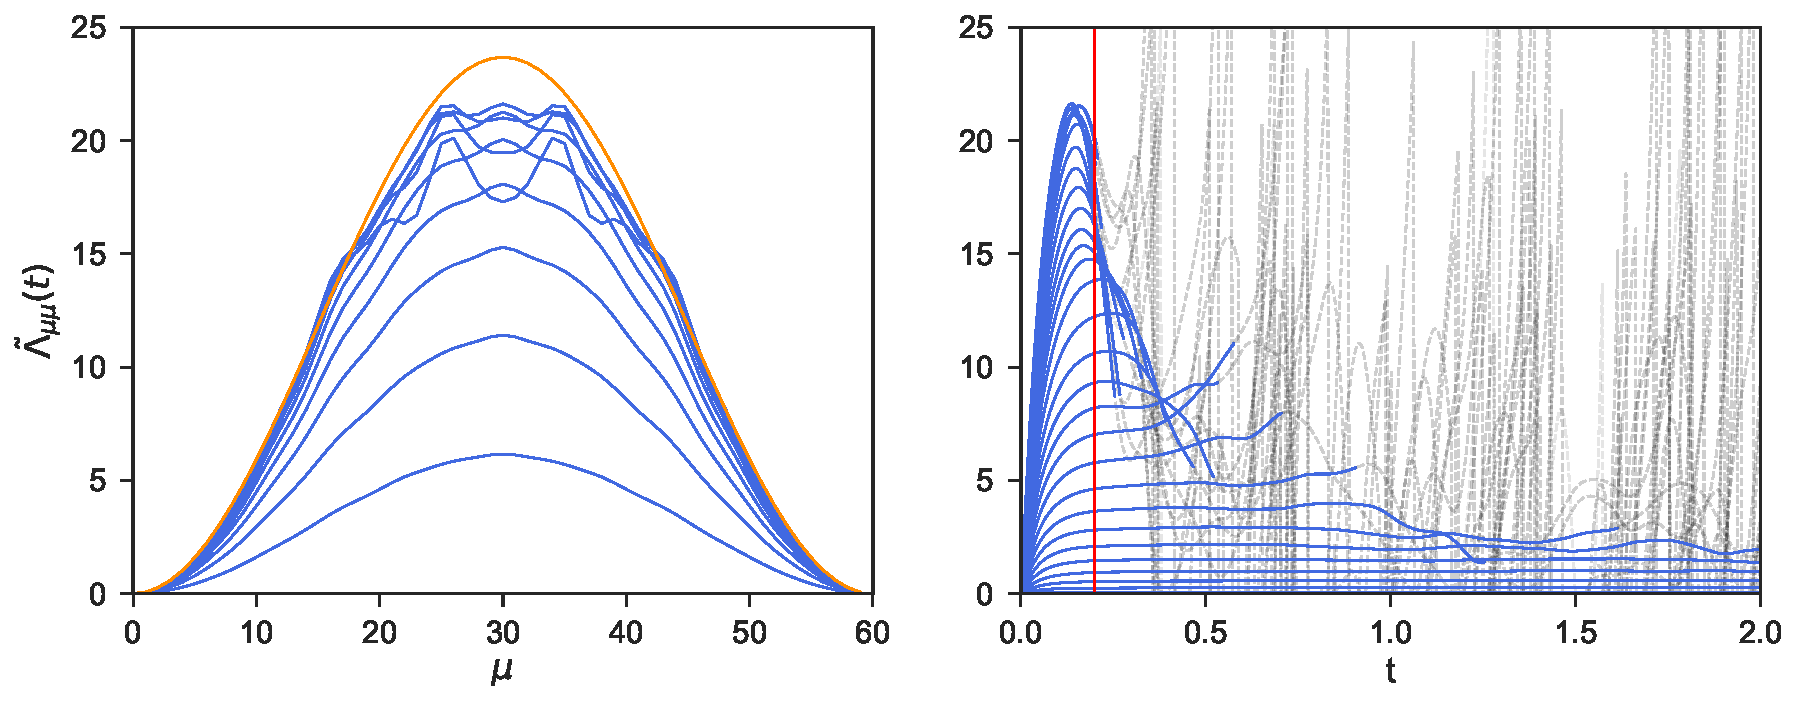
\includegraphics[scale=0.45]{LambdatFourier-PBC}
\caption[Diagonal elements  $\tilde{\Lambda}_{\mu\mu}(t)$ of  the Fourier transform of $\Lambda(t)$]{The  diagonal elements  $\tilde{\Lambda}_{\mu\mu}(t)$ of  the
  Fourier transform of $\Lambda(t)$ defined in (\ref{AproxCtau}), as a
  function of  $\mu$ (left)  and $t$  (right).  In  the top  panel, in
  ascending  order the  plotted times  go  from $t=0$  to $t=0.20$  in
  intervals of $0.02$.  The dotted line is the local approximation Eq.
  (\ref{Lambdaloc}) with a  value of the local  kinematic viscosity of
  $\nu_0=1.48$.   In the  right panel,  we observe  a clear  plateau,
  beyond  $\tau=0.2$  indicating  the  exponential  behaviour  of  the
  correlations in Fig. \ref{fig:CtFourier-PBC-exp}.}
\label{fig:LambdatFourier-PBC}
\end{figure}

In       Fig.         \ref{fig:LambdatFourier-PBC}       we       plot
$\tilde{\Lambda}_{\mu\mu}(t)$  as a  function of  $\mu$ for  different
times (left) and as a function of $t$ for the different values of $\mu$
(right). In the left panel,  the different curves correspond to values
of  $t$ from  $0$ to  $0.20$ in  intervals of  $0.02$.  The  structure
observed  in the  central region  is spureous  and due  to statistical
errors.   These   errors  increase  with   time.   We  also   plot  in
Fig. \ref{fig:LambdatFourier-PBC}  the theoretical prediction  of this
matrix in the local approximation  given in Eq. (\ref{taumuloc}) for a
fitted value  of the  local kinematic  viscosity of  $\nu_0=1.48$. \Pendiente{This value corresponds to the kinematic viscosity of a fluid with density $\rho=0.6$ and temperature $T=2.0$ \cite{Woodcock2006}}.  We
observe that  the local approximation (\ref{taumuloc})  gives a fairly
reasonable approximation  for the converged  value $\tilde{\Lambda}^*$
of the  relaxation matrix in Fourier  space.  In the right  panel, we
plot $\tilde{\Lambda}_{\mu\mu}(t)$ for all $\mu$ as a function of time
$t$.  We  have disregarded the data  points beyond times in  which the
statistical  errors  lead  to  meaningless results  (those  below  the
threshold  in  the  eigenvalues  in Fig  \ref{fig:CtFourier-PBC-exp}).   We  may
appreciate a  very clear  plateau for  the modes  of low  $\mu$ (large
wavelengths).  As the wavenumber increases, for wavenumbers $\mu\ge20$
the plateau dissappears  and this is concomittant  with the appearance
of great distorsions that are due  to the lack of statistics necessary
to describe  the inverse  of the correlation matrix.  Therefore, we  cannot decide
from the plots  wether there is no plateau at  large wavenumber or, on
the contrary,  there is a  plateau but it is  obscured by the  lack of
statistics.  A clear convergence of $\tilde{\Lambda}_{\mu\mu}(t)$ to a
constant  plateau  value  $\tilde{\Lambda}^*$ is  observed  for  times
larger than $t\simeq  2$. Therefore, we select the  time $\tau=0.2$ as
the best compromise  satisfying that $\tilde{\Lambda}_{\mu\mu}(t)$ has
attained  its  constant  value  but  does  not  suffer  from  dramatic
statistical errors.     The existence  of a  plateau
beyond  $\tau=0.2$  signals  to   the  exponential  behaviour  of  the
correlations  in  Fig.   \ref{fig:CtFourier-PBC-exp}  beyond  this  time.   We
measure  then   the  relaxation   matrix  in  Fourier   space  through
$\tilde{\Lambda}^*_{\mu\mu}=\tilde{\Lambda}_{\mu\nu}(\tau)$.      This
measured relaxation  matrix is  compared with its  local approximation
$\tilde{\Lambda}^{\rm loc}_{\mu\mu}$ which, from Eq. (\ref{taumuloc}),
is given by
\begin{align}
\tilde{\Lambda}^{\rm loc}_{\mu\mu}&=\frac{2}{\Delta z^2}
\left(1-\cos\left( \frac{2\pi \mu}{N_{\rm bin}}\right)\right)
\nu_0
\label{Lambdaloc}
\end{align}

\begin{figure}[h!]
  \centering
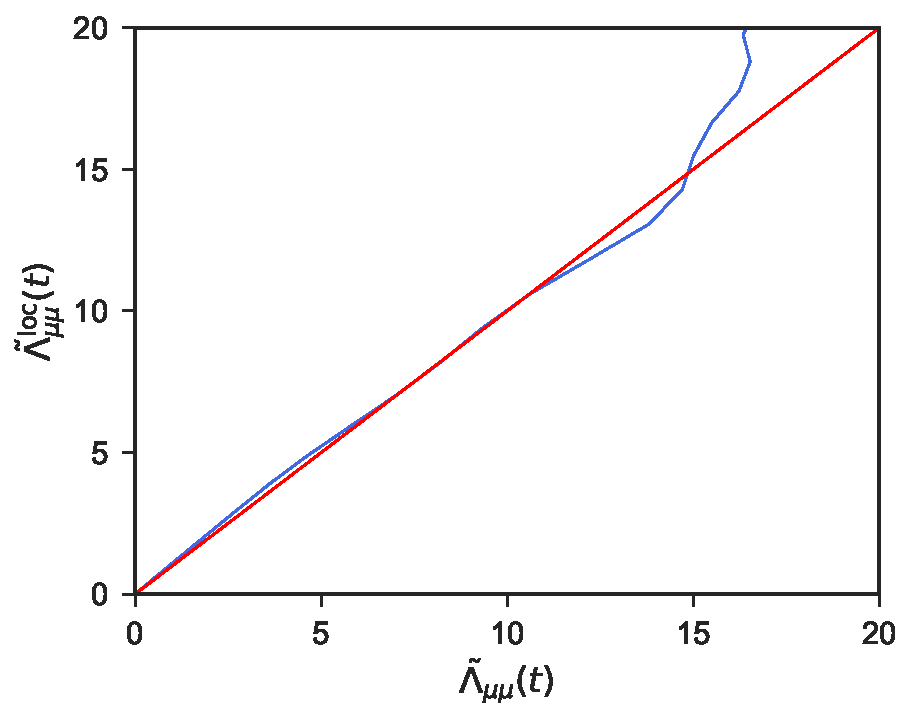
\includegraphics[scale=0.45]{CompareLambdas-PBC}
\caption[Comparison $\tilde{\Lambda}^*_{\mu\mu}$ and $\tilde{\Lambda}_{\mu\mu}(\tau)$]{Comparison $\tilde{\Lambda}^*_{\mu\mu}=\tilde{\Lambda}_{\mu\mu}(\tau)$ for $\tau=0.2$ with $\tilde{\Lambda}^{\rm loc}_{\mu\mu}$ in Eq. (\ref{Lambdaloc}) with $\nu_0=1.48$. The red line has slope $1$ and it is for guide the eye.}
\label{fig:CompareLambdas-PBC}
\end{figure}
In         Fig.           \ref{fig:CompareLambdas-PBC}         we         plot
$\tilde{\Lambda}^*_{\mu\mu}=\tilde{\Lambda}_{\mu\mu}(\tau)$        for
$\tau=0.2$    against    $\tilde{\Lambda}_{\mu\mu}^{\rm    loc}$    in
(\ref{Lambdaloc})   with  $\nu_0=1.48$. Observe that the linear behaviour of this plot
indicates  that,  to  a  very good  degree,  the  local  approximation
describes well the relaxation matrix $\Lambda^*$.
From the Fourier transform  of the diagonal matrix $\tilde{\Lambda}^*$ i
we may  obtain the relaxation  matrix $\Lambda^*$ in real space which,  by comparing
(\ref{AproxC})      with     (\ref{SDECpi})      is     given      by
$\Lambda^*=\Delta\nu^*$. From Eq.  (\ref{Cmunut}) we can
now  have the  prediction of  Mori theory  for the  correlation matrix
$C(t)$.  In Fig.  \ref{fig:Predictionsmumu-PBC} we compare the autocorrelation
$C_{\mu\mu}(t)$ measured in  MD with the predictions  of the nonlocal
(orange) and local  (green) theories.  The arrow is at  $t=\tau$ where the
three curves  coincide by  construction.  The  agreement of  the three
curves  is  excellent beyond  $\tau$.   This  is best  appreciated  in
logscale (right panel). The curving at long times,
reflecting the  finite size  of the simulation  box \Pendiente{(see  appendix)} is
captured in  both theories.  The inset  in the left panel of Fig.  \ref{fig:Predictionsmumu-PBC}
shows a zoom at short times,  where one appreciates that the nonlocal
theory gives  a better  prediction than the  local prediction  but, of
course,  yields  poor results  at  very  short  times. Note  that  the
Markovian theory leads to a cusp at $t=0$ in the correlation while the
MD  results  have   a  vanishing  value  of  the   derivative  of  the
correlation.

\begin{figure}[h!]
  \centering
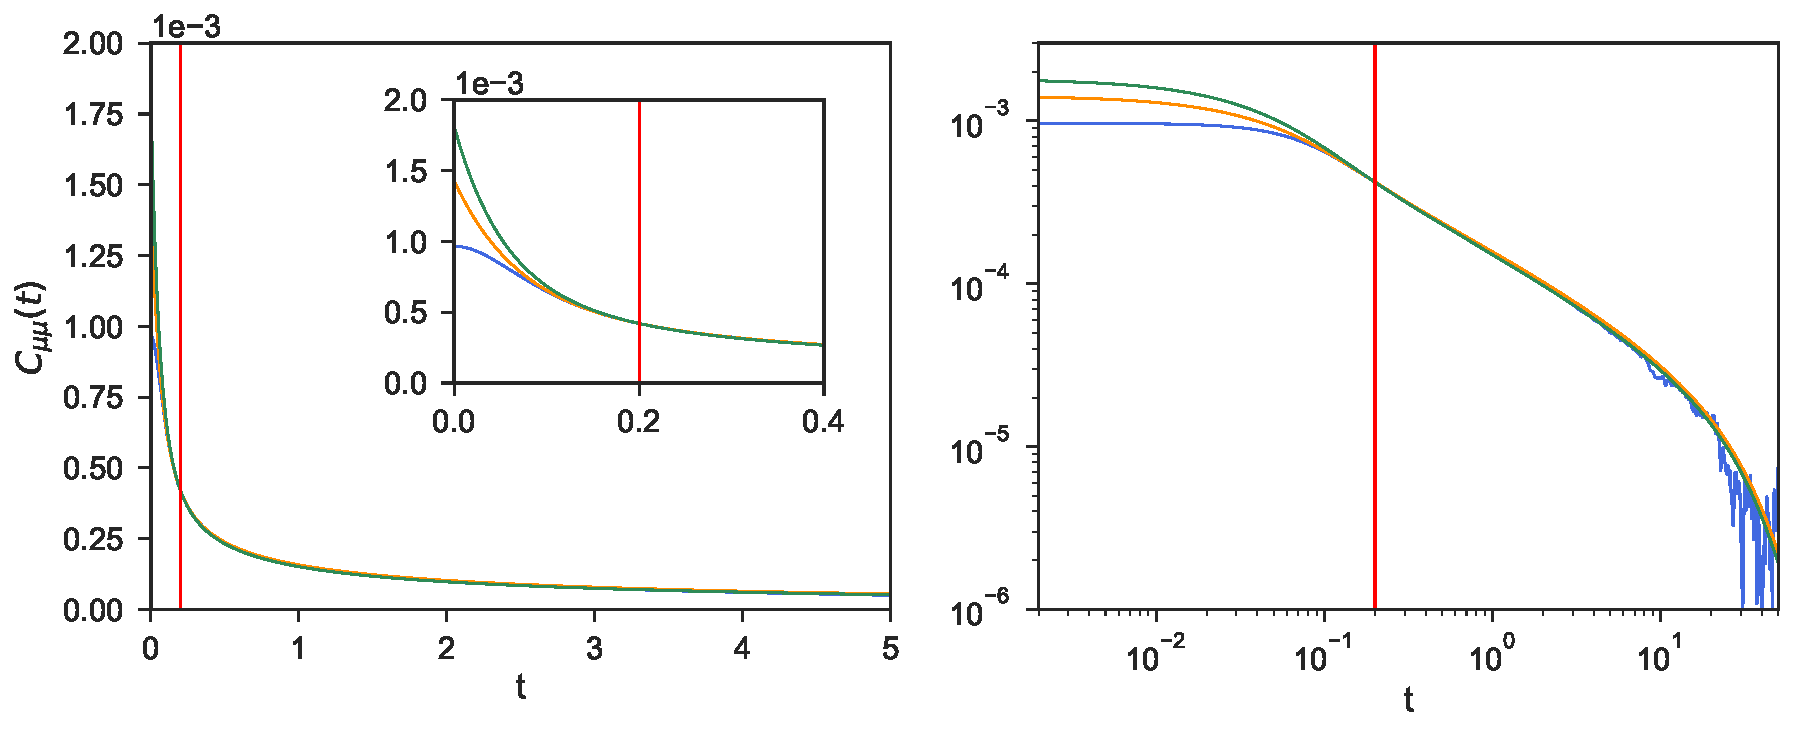
\includegraphics[scale=0.45]{Predictionsmumu-PBC}
\caption[Comparison of autocorrelation $C_{\mu\mu}$ with the predicions for PBC system]{Comparison of autocorrelation $C_{\mu\mu}(t)$ with the predictions of the nonlocal (orange) and local (green) theries. The left panel is in linscale and the right panel in logscale. The red line is at $t=\tau$ where the three curves coincide by construction. The inset shows a zoom at short times.}
\label{fig:Predictionsmumu-PBC}
\end{figure}

In Fig. \ref{fig:Predictionsmumu+1-PBC} we compare the cross correlation $C_{\mu\mu+1}(t)$ in the same way as we did with the autocorrelation in Fig. \ref{fig:Predictionsmumu-PBC}. The agreement of the the three curves (predictions, nonlocal and local theories) is excellent beyond $\tau$, but we appreciate that for long times \Note{the local prediction is better than the nonlocal prediction}. 

\begin{figure}[h!]
  \centering
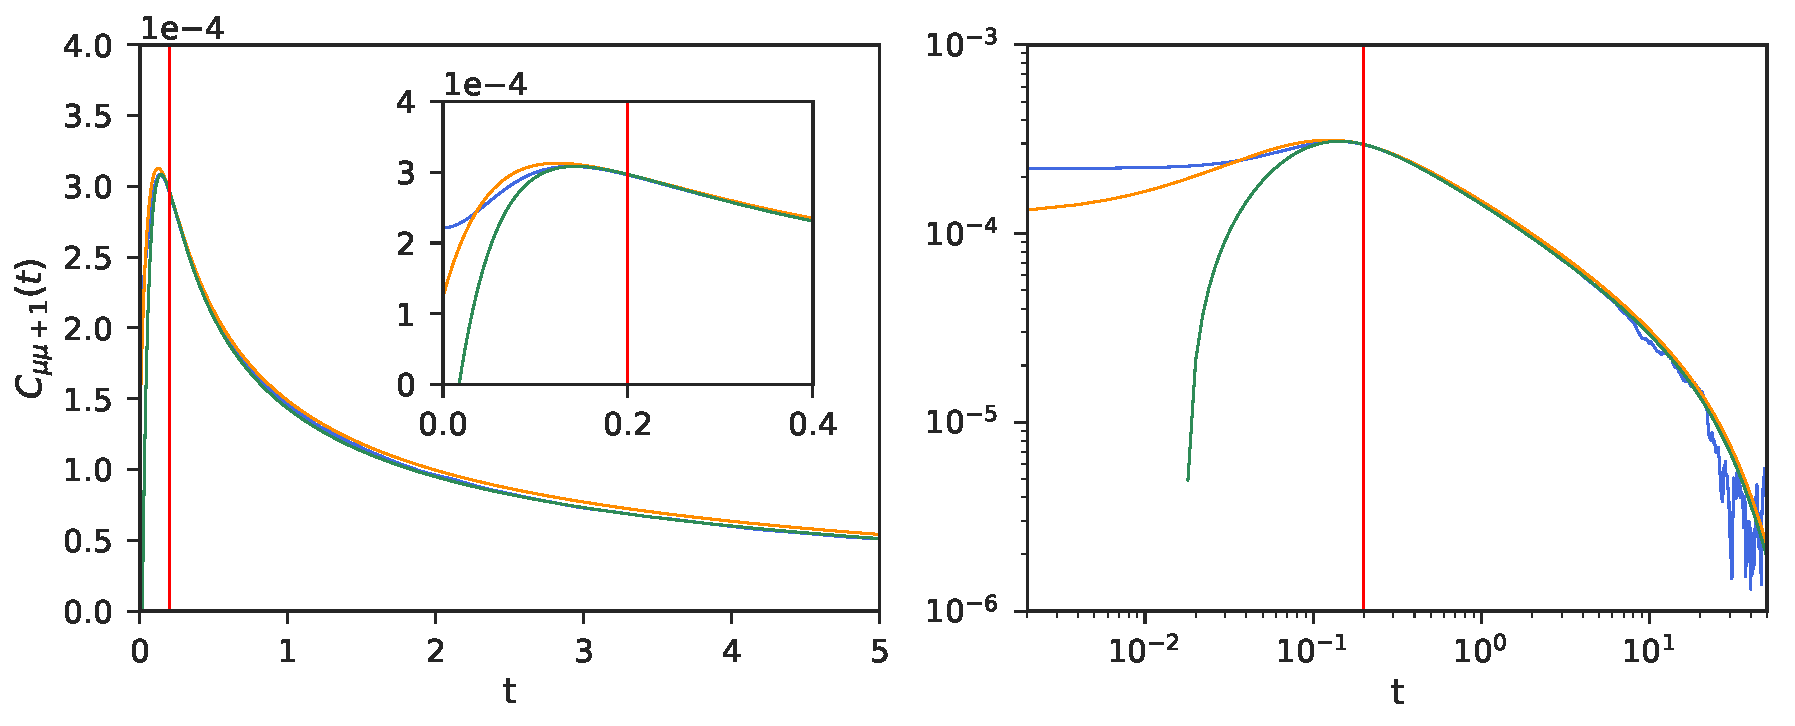
\includegraphics[scale=0.45]{Predictionsmumu+1-PBC}
\caption[Comparison of cross correlation $C_{\mu\mu+1}$ with the predicions for PBC system]{Comparison of autocorrelation $C_{\mu\mu+1}(t)$ with the predictions of the nonlocal (orange) and local (green) theries. The left panel is in linscale and the right panel in logscale. The red line is at $t=\tau$ where the three curves coincide by construction. The inset shows a zoom at short times.}
\label{fig:Predictionsmumu+1-PBC}
\end{figure}

In summary, in the present subsection we have shown that the Markovian
approximation  is  an   excellent  one  for  the   prediction  of  the
correlation matrix of the  transverse momentum beyond a characteristic
time $\tau$.   We have also  observed that, \textit{beyond}  this time
$\tau$,  a  local  in  space  approximation  gives  equally  excellent
predictions.




\subsection{The Green-Kubo nonlocal viscosity matrix}
In   this  section,   we  discuss   the  nonlocal   viscosity  matrix
$\eta_{\mu\nu}(\tau)$  defined   Eq.   (\ref{non-loc}).    To  compute
$\eta_{\mu\nu}(t)$   we    record   the   stress   tensor    per   bin
$\hat{\sigma}_\mu$,  defined in  (\ref{sbin}),  and  compute the  time
integral     of     the      equilibrium     correlation     $\llangle
\hat{\sigma}_{\mu}(t)\hat{\sigma}_\nu\rrangle$.         In        Fig.
\ref{fig:Etat-PBC}  we  plot  the nonlocal  shear  viscosity
matrix  $\eta_{\mu\nu}(t)$  for  $\mu=30$   and  different  values  of
$\nu=30-40$.   We observe  that  $\eta_{\mu\nu}(t)$ starts  from 0  at
$t=0$  and  attains a  maximum  at  a  time  that increases  with  the
separation between bins. Even though in linear scale there seems to be
a plateau after the maximum, the logscale representation in the bottom
panel of Fig.  \ref{fig:Etat-PBC} reveals that such a plateau
does  not exist  as a  very slow  algebraic decay  is apparent.   This
result reveals strikingly that  the standard Green-Kubo expression for
the nonlocal  viscosity has no plateau  and cannot be used  to define
the nonlocal viscosity  because there is no a priori  criteria to fix
the  upper  limit   of  integration  $\tau$.   Of   course,  from  Eq.
(\ref{etaExact})  we already  observed  that $\eta(t)$  cannot have  a
plateau because the time derivative of the correlation function decays
at  long times.   Note  that the  non-existence of  a  plateau in  the
nonlocal viscosity matrix $\eta(t)$ is  in clear contrast to the case
of  the Green-Kubo  running  integral for  the  local shear  viscosity
$\eta_0(t)$ which,  according to Eqs.  (\ref{eta00})  and (\ref{etat})
is proportional to the sum of all the function $\eta_{\mu\nu}(t)$ that
decay  in a  quasi  algebraic  manner. 

\begin{figure}[h!]
  \centering
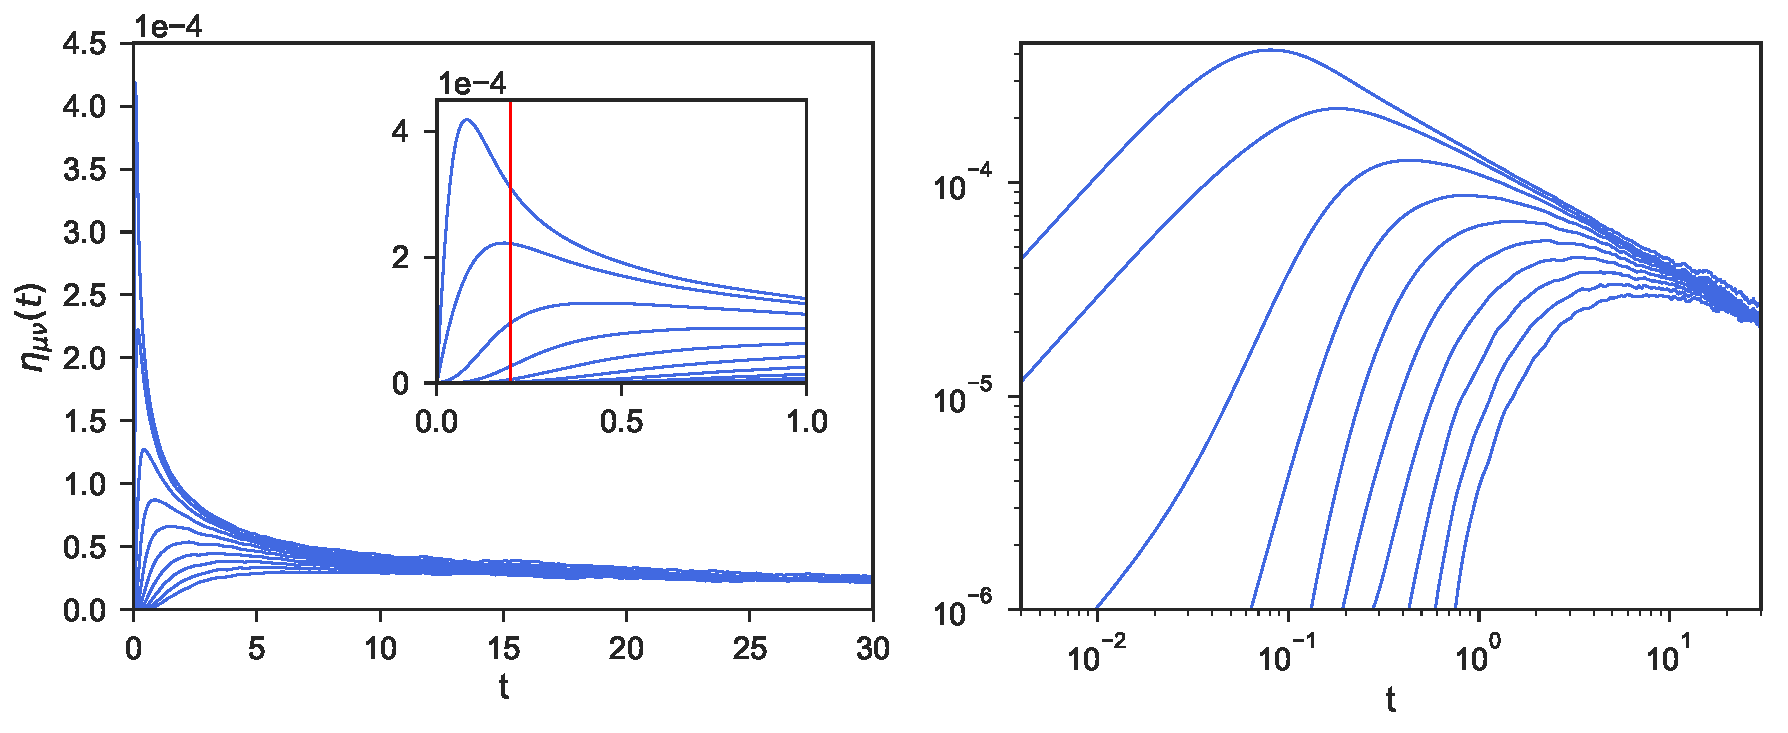
\includegraphics[scale=0.45]{Etat-PBC}
\caption[The nonlocal viscosity as a function of time for PBC system]{The nonlocal viscosity $\eta_{\mu\nu}(t)$ as a function of time, for $\mu=30$ and, in descending order, $\nu=30-40$. The left panel is in linscale, while the right panel in logscale. The inset is a zoom and the red line is at $t=\tau$.}
\label{fig:Etat-PBC}
\end{figure}


In Fig.
\ref{fig:KinVisc0t-PBC} we plot $\nu_0(t)$  which we recall that
is the sum  of the curves in  the left panel of Fig. \ref{fig:Etat-PBC} divided by the density. We observe  a very neat
plateau.  Of course, the plateau cannot extend indefinitely because of
the  finite number  of terms  involved  in the  sum (\ref{eta00}).  \Note{ Entnder bien :We
expect that after  an estimated time of the order  of $L^2/\nu_0$ that
takes the vorticity to diffuse the entire system size the plateau will
curve down.  In our system  this time is  $\sim 600$, well  beyond our
observation  span. After  this  time  we expect  that  the plateau  in
$\nu_0(t)$ will start to decrease due to finite size effects.}
\begin{figure}[h!]
  \centering
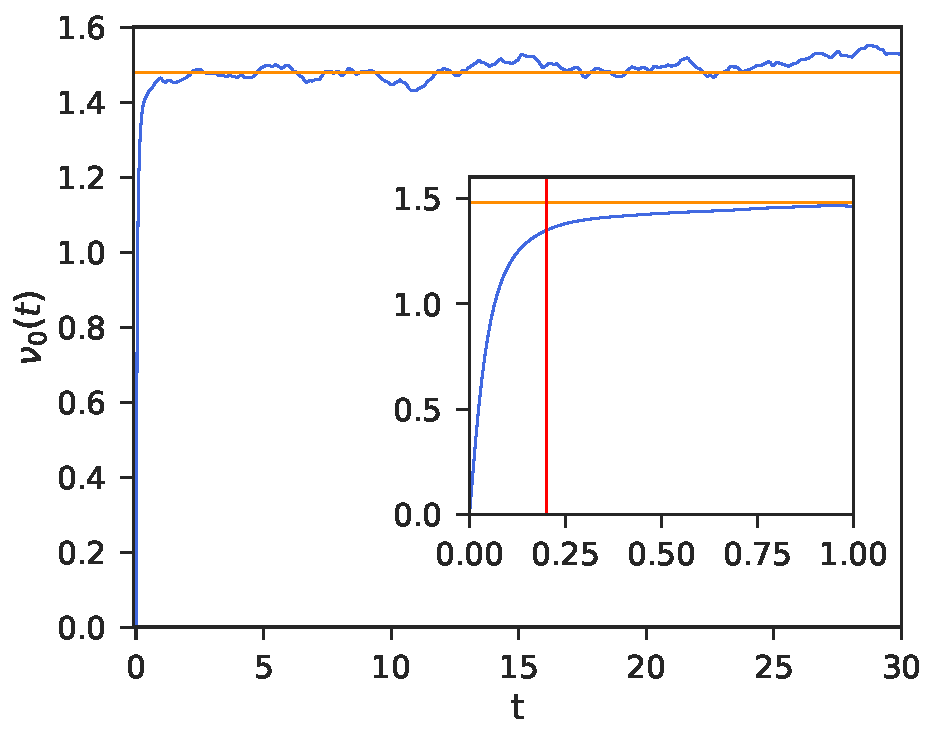
\includegraphics[scale=0.45]{KinVisc0t-PBC}
\caption[The local kinematic viscosity for PBC system]{The local kinematic viscosity $\nu_0(t)=\eta_0(t)/\rho^{\rm eq}$ as a function of time where the shear viscosity is computed with the data from Fig. \ref{fig:Etat-PBC}. A horizontal orange line at $\nu_0=1.48$ is also plotted in order to guide the eye in the plateau region.}
\label{fig:KinVisc0t-PBC}
\end{figure}

By following a  strategy similar to the one given  in Sec. \ref{Sec:Mori} \Note{Sección o referenciar paper?} we
have shown in  Eq. (\ref{FouFin}) how to evaluate  the nonlocal shear
viscosity  matrix  $\tilde{\eta}^*_{\mu\mu}$  not  from  the  standard
Green-Kubo  formula but  rather from  a corrected  version of  it that
accounts for the  fact that the Green-Kubo running  integral decays as
the correlation of  the CG variables themselves. In  order to evaluate
$\tilde{\eta}^*_{\mu\mu}$ we introduce the time dependent eigenvalue
\begin{align}
\tilde{\eta}_{\mu\mu}^*(t)&=\frac{\tilde{\eta}_{\mu\mu}(t) }{\tilde{c}_{\mu\mu}(t)}
\label{FouFint}
\end{align}
which, according  to Eq. (\ref{FouFin})  should have a plateau  if the
Markovian approximation is appropriate.

In    Fig.      \ref{fig:EtaStartFourier-PBC}    we    show     the    function
$\tilde{\eta}_{\mu\mu}(t)$  as a  function of  time for  the different
modes.   We observe  that, whenever  the  statistics allow  for it,  a
reasonable plateau  is obtained. Therefore,  it is possible  to define
the  nonlocal  shear  viscosity  matrix  $\eta^*_{\mu\nu}$  from  the
Fourier transform  of the plateau  value $\tilde{\eta}_{\mu\mu}(\tau)$
where $\tau=0.2$.  This  is shown in Fig.  \ref{fig:CompareEtas-PBC} where the
diagonal structure  is apparent,  with a width  that has  around $\sim
5\sigma$.  This  is, approximately  twice the  cutoff distance  of the
Lennard-Jones potential.  One way to  explain this width is  by noting
that  the stress  tensor of  a bin,  defined in  (\ref{sbin}) contains
contributions of pairs  of atoms through the fraction  of the distance
between the atoms. Bins which are  at a distance larger than twice the
LJ cutoff radius  do not have any atom  that simultaneously contribute
to the stress tensor in each  bin. Therefore, it is plausible to infer
that the width of the stress correlation is a consequence of the absence
of correlation between the stress through atoms that contribute to the stress
in both bins.


The kinematic viscosity  in Fourier space is  obtained by transforming Eq. (\ref{numunu0})
to Fourier space  and gives
\begin{align}
\tilde{\nu}_\mu(t)&=  \frac{{\cal V}_\mu \tilde{\eta}_\mu(t)}{\tilde{\rho}_\mu}
  \label{kinViscFourier}
\end{align}
We plot $\tilde{\nu}_\mu(t)$  in Fig.  (\ref{fig:KinVisctFourier-PBC}) as a  function of time
$t$ for  different modes  $\mu$ (left)  and as a  function of  the mode
number $\mu$  at different times from $t=0$ to $t=0.2$ in intervals of $0.01$ (right). From
the last plot  we observe that the modes around  $\sim 30$ are subject
to  large statistical  error because  for these  modes the  eigenvalue
$\tilde{c}_\mu(t)$ of  the correlation  matrix has already  taken very
low values, thus  amplifying though its inverse  the small statistical
errors present. In  any case, we observe  that $\tilde{\nu}_\nu(t)$ is
almost constant for all values of $\mu$ and that for times larger than
$\tau=0.2$ the  kinematic viscosity  of all  modes is  fairly constant
$\tilde{\nu}_\nu(\tau)\simeq\nu_0=1.48$  in  reduced units.  This  is,
another reflection  of the  fact that the  discrete hydrodynamics in 
periodic boundary conditions is fairly local, and can be described with
 a local in space approximation, as has been corroborated in Figs. 
 \ref{fig:Predictionsmumu-PBC}, \ref{fig:Predictionsmumu+1-PBC} and \ref{fig:EtaStartFourier-PBC}.


\begin{figure}[h!]
  \centering
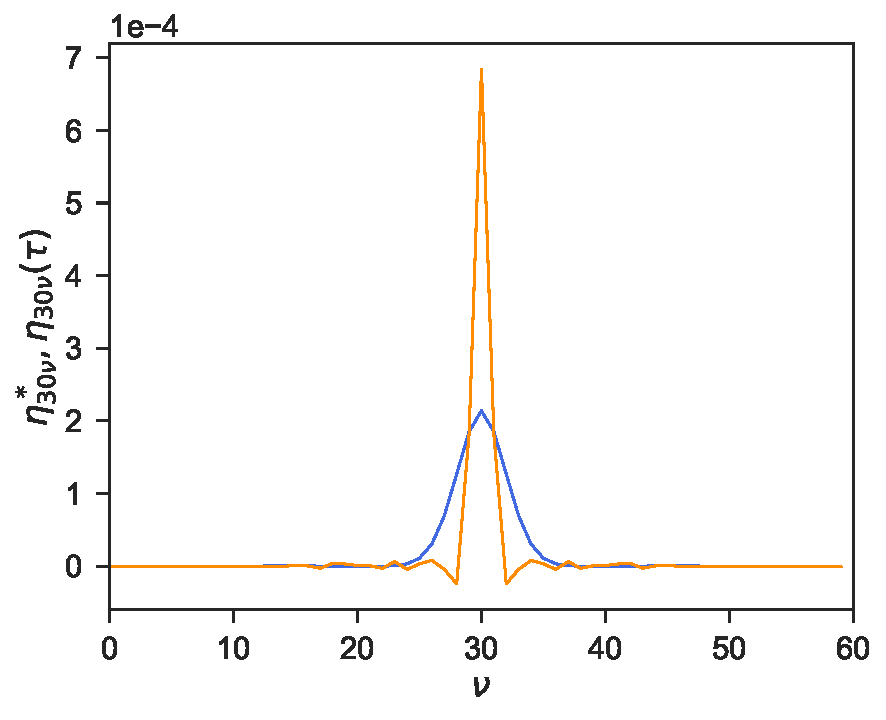
\includegraphics[scale=0.45]{CompareEtas-PBC}
\caption[Comparison $\eta^*_{30,\nu}$ and $eta_{30,\nu}$]{The nonlocal shear viscosity $\eta_{\mu\nu}$ (blue) and its corrected form $\eta^*_{\mu\nu}$ (orange) for $\mu=30$ as a function of node index $\nu$ at $t=0.2$.}
\label{fig:CompareEtas-PBC}
\end{figure}



\begin{figure}[h!]
  \centering
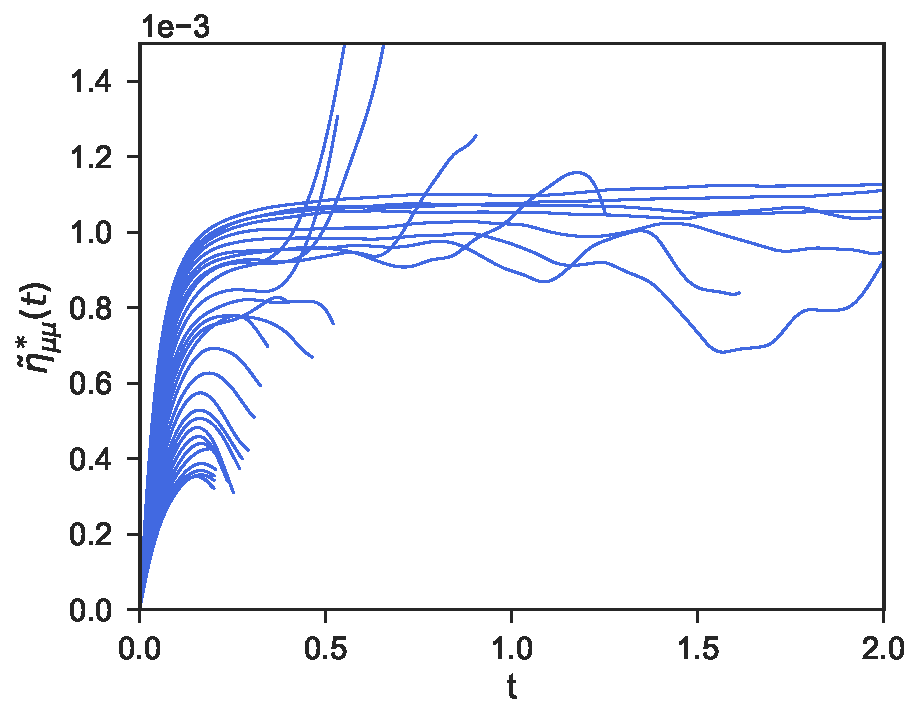
\includegraphics[scale=0.45]{EtaStartFourier-PBC}
\caption[The nonlocal shear viscosity kernel for PBC system]{The nonlocal shear viscosity kernel from corrected Green-Kubo formula $\tilde{\eta}^*_{\mu\mu}=\frac{\tilde{\eta_{\mu\mu}(t)}}{\tilde{c}_{\mu\mu}(t)}$}
\label{fig:EtaStartFourier-PBC}
\end{figure}
\begin{figure}[h!]
  \centering
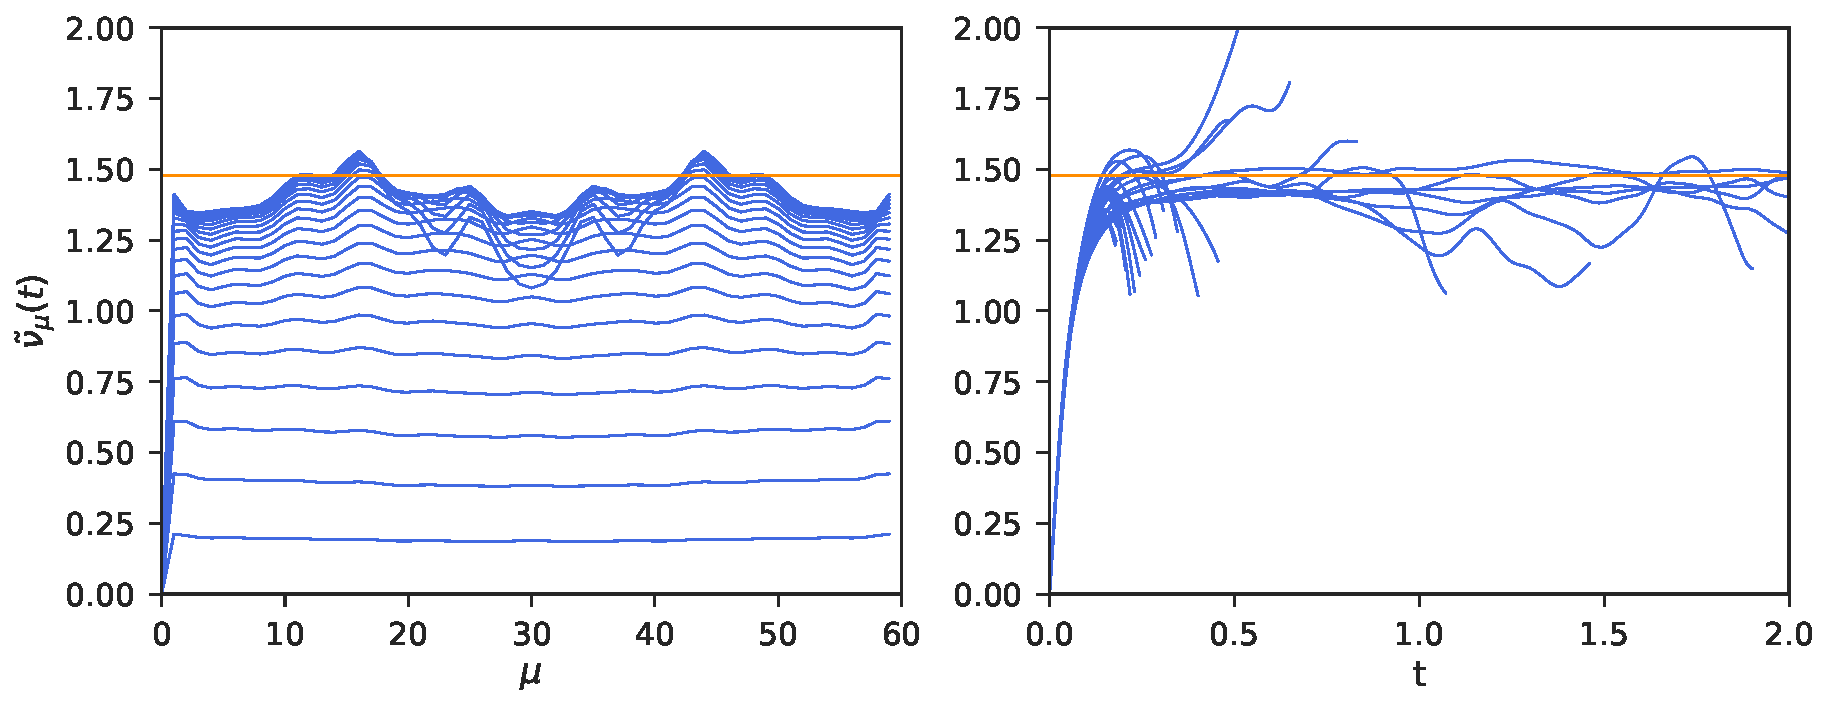
\includegraphics[scale=0.45]{KinVisctFourier-PBC}
\caption[The eigenvalues of the nonlocal kinematic viscosity matrix for PBC system]{The eigenvalues of the nonlocal kinematic viscosity matrix defined in Eq. (\ref{kinViscFourier}) as a function of time (right panel), and as a function of the mode index por times from t=0 to t=0.2 in ascending order in intervals of $0.01$. The orange line at $\nu_0=1.48$ is plotted in order to guide the eye in the plateau region.}
\label{fig:KinVisctFourier-PBC}
\end{figure}

\newpage
\section{Conclusions}
\label{Sec:ConclusionsChapPBC}
In the first part of this chapter -- Sec. \ref{Sec:Mori} -- we have addressed  the plateau problem that  appears in
the  expression of  transport  coefficient in  terms  of the  standard
Green-Kubo running integrals.  In the  case of Markovian dynamics with
not an extreme separation of time  scales, the decay of the Green-Kubo
running integral does  not allow to determine  unambiguously the value
of the  transport coefficients.  We  have shown in  Eq.  (\ref{Math1})
that  the  Green-Kubo  running  integral necessarily  decays  to  zero
because it  is given in terms  of the correlation of  the CG variables
and its  time derivative.  With  this observation, we have  proposed a
correction  to  the  standard  Green-Kubo  expression  that  does  has  a
well-defined infinite time limit. We have seen also that it is crucial
to  distinguish between  the  three  different ``friction  matrices'':
$M(t)$ involving the real dynamics (that  goes to zero as time goes to
infinity), $M^+(t)$  involving the projected dynamics  (that also goes
to zero  with time  going to  infinity, in  spite of  claims otherwise
\cite{Kubo1991,Espanol1993}),  and $M^*$,  a putative  constant
matrix   given    by   the    non-zero   infinite   time    limit   in
Eq. (\ref{GKCorrected}).


In the second part of this chapter -- Sec. \ref{Sec:MoriPBC} and Sec. \ref{Sec:SimPBC} --  we  have computed from  MD simulations  the equilibrium
time-dependent correlation matrix of  the discrete transverse momentum
density.   Under  the Markovian  approximation,  Mori  theory gives  a
definite prediction for the correlation  matrix in terms of a decaying
matrix exponential.   As we  have discussed in Sec. \ref{Sec:MarkovianAprox}, the  Markovian prediction
\textit{cannot}  hold for  very small  times. Only after a time $\tau$ in which the memory
has fade out one can expect a Markovian approximation to hold. We validated it though MD simulations in Sec. \ref{Sec:ValidateMarkovPBC}.


A number of conclusions can be drawn from the simulation results:
\begin{enumerate}
\item We  have observed that  the relaxation matrix  $\Lambda(t)$ does
  indeed  plateau to  a  constant value  $\Lambda^*$, indicating  that
  after  the  time $\tau$  the  decay  of  the correlation  matrix  is
  exponential  and  hence Markovian. This  time  is not  excessively
    large, capturing about  80\% of the total decay  of the correlation.
  The  Markovian approximation  predicts a  quasi-algebraic long  time
  tail  that gives  excellent agreement  with the  simulation results.
  Trully algebraic  decay is  obtained only  in the  thermodynamic and
  continuum limits, as described  in Appendix \ref{Ap:Cont}. Note that
  the width  of the bins  that we use in  the present work  is $\Delta
  z=0.5\sigma$.  Such bin  size allows,  in the  presence of  walls to
  resolve the density layering near the wall.
\item  We observe  that  for  the times  beyond  $\tau$  in which  the
  Markovian (local in time) approximation is valid, the local in space
  approximation of the kinematic  shear viscosity matrix gives already
  very accurate results.
\item The \textit{nonlocal}  shear viscosity defined in  terms of the
  Green-Kubo  formula  as  the  time  integral  of  the  stress-stress
  correlation does  not show a  plateau. Quite remarkably, the  sum of
  the  (non-plateau) nonlocal  shear viscosity  matrix elements  does
  indeed   have  a   plateau.    This  plateau   corresponds  to   the
  \textit{local}  viscosity  computed  in   the  usual  way  from  its
  Green-Kubo  formula. The  existence  of this  plateau  in the  local
  viscosity is due to global momentum conservation.
\end{enumerate}
These facts suggest that the usefulness of a nonlocal shear viscosity
in a  Markovian description  of correlation functions  of hydrodynamic
variables is small.  On one hand, its Green-Kubo expression is useless
as it does not have a plateau and, on the other, a local approximation
with well-defined plateau already provides excellent results.

Steady states situations in which the Markovian approximation is valid
automatically may  still require the  use of nonlocal in  space shear
viscosities for its correct description \cite{.}.

In  this chapter  we  have  limited  ourselves to  the  discrete
transverse  momentum   variable.   With  the  same   methodology,  the
extension  to   the  rest  of  conserved   hydrodynamic  variables  is
straitghforward and will be presented elsewhere. 

One strategy to increase the validity of a purely Markovian theory for
times   smaller  than   $\tau$   consists   on  including   additional
non-conserved variables in the list  of CG variables.  For example, by
including the stress tensor and heat flux as additional variables, one
expects  to  capture the  viscoelastic  and  memory effects  that  are
required to describe the dynamics  of the conserved variables at small
time scales \cite{Khayat1989,mryglod1995,Bryk2010}.

Despite of considering the simplest case such as  simple fluid  in periodic  boundary conditions, the  same methodology used here  will be  used in the following chapters for  the case  of fluids
confined in between parallel solid walls.  The computational burden in
that case is much larger  because traslation invariance cannot be used
in order to increase statistics.
In  addition   to  the   nonlocal  shear  viscosity,   new  transport
coefficients related to slip at the wall appear in confined fluids, as
Camargo et al. presented in \cite{CamargoBC2018}.


%-----------------------------------------------------------------
% CHAPTER 5
%-----------------------------------------------------------------
\chapter{Markovian behaviour near solids}\label{Chap:Walls}
\markboth{Markovian behaviour near solids}{}
\epigraph{\textit{Descubrir es ver de otro modo lo que nadie ha percibido.}}{Blanco Nocturno \\ RICARDO PLIGIA}
\section{Introduction}
In Chapter \ref{Chap:PBC} we have demonstrated
through MD simulations that the Markovian assumption
is  valid  for  the  description   of  correlations  of  the  discrete
transverse momentum \textit{beyond} certain  time.  We have shown that
beyond  this   time,  hydrodynamics  is  essentially   local  in  time
\textit{and} space.  
In this chapter we follow the same strategy as for unconfined fluids in order to study the Markovian behaviour of a fluid in between two solid slabs. 


As we mentioned in the introduction to Chapter \ref{Chap:PBC}, at nanoscopic scales,  a fluid
starts displaying its  molecular structure in phenomena  like the wall
ordering.   In  addition, slip  of  the  fluid  at the  walls  becomes
noticeable.   The  usual  local hydrodynamic  description  with  local
transport coefficients  and no  slip boundary  conditions needs  to be
adequately modified in  order to address the  peculiar fluid behaviour
at  nanoscales. Slip  at nanoscales  has  received a  large amount  of
attention from the simulation point  of view since the pioneering work
of Thomson and Robins \cite{Thompson1990,Koplik1995,Troian1997}.

We  have presented  in  Chapter \ref{Chap:Theory}  a  derivation of  the
equations of hydrodynamics in the  presence of solid walls that govern
the  averages of  the  mass  and momentum  density  fields. A  crucial
feature of this theory is that the effect of the walls on the fluid is
not through boundary conditions but  rather through forces confined to
the vicinity  of the solid wall.  In a recent work, Camargo et al. \cite{CamargoBC2018} showed  how  boundary  conditions  can  be  derived  when  the  flows  are  of
macroscopic  character.  The  theory  gives  the usual  Navier  slip
boundary  condition  with   microscopically  defined  parameters  that
coincide      with      those      of     Bocquet      and      Barrat
\cite{Bocquet1994}.

The only crucial  assumption made in the formulation of  the theory in
Chapter \ref{Chap:Theory} is  that the dynamics  is Markovian, this  is, that
the hydrodynamic equations do not  have integral memory terms.  It is,
therefore, important to test through MD simulations that the Markovian
approximation is  correct.  Comparison with MD  simulation require the
introduction  of discrete  equations. To  achieve this  goal, we  have
proposed in Chapter \ref{Chap:Planar} a  discrete hydrodynamic theory  for planar
flows near  solid walls  that can  be understood  as a  finite element
discretization of  the continuum  theory presented in Chapter \ref{Chap:Theory}.
The size of the bins enter  the discrete theory as an intrinsic length
scale. The forces on fluid elements are due to the effect of non-local
stress tensor and non-local surface forces due to the walls.

In the  theory presented in Chapter \ref{Chap:Theory}, based  on the
projection  operator technique,  the Markovian  approximation produces
formal expressions in  terms of Green-Kubo formulae  for the transport
coefficients.    However  these   expressions  are   formal  for   two
reasons. First they involve the  so called projected dynamics which is
uncomputable from MD  simulations. The usual step  of substituting the
projected dynamics  by the real  Hamiltonian dynamics is  not entirely
justified. The second  problem is that the  Green-Kubo formulae suffer
from the plateau problem \cite{Kirkwood1949,Espanol1992}.  
In Sec. \ref{Sec:CorrectedGK} we have  presented a   new  corrected   Green-Kubo  expression   for  transport
coefficients that does not suffer from the plateau problem.

The  theory presented  in Chapter \ref{Chap:Theory} describes  the
evolution of non-equilibrium ensemble averages  and it is based on the
Kawasaki-Gunton  projector \cite{Grabert1982}.   It is  non-linear and
involves the  free energy functional familiar  from Density Functional
Theory.  For the case of  the transverse momentum, the Kawasaki-Gunton
projector gives  a very simple  linear equation that does  not involve
the free  energy functional.   A very similar  linear equation  can be
obtained  in an  alternative way  from the  simpler Mori  theory, that
always produces  linear equations.   In order  to address  the plateau
problem  it proves  very  convenient to  have a  theory  not only  for
averages but also for time correlation functions and both are provided
in Mori theory.  


\section{The CG variables and its dynamics}
We  consider a  LJ  fluid system  confined  in between  two
parallel solid walls made of LJ particles fixed in a simple
cubic lattice as is represented in Fig. \ref{fig:WallsBox}. The walls are  along the directions $x^1,x^2$.  Because
of  traslational  invariance along  the  walls,  we bin  the  vertical
direction $x^3$ in layers paralel to  the planar walls. In the same way as was exposed in Sec. \ref{Sec:CGVariablesPBC} the box length
$L_z$ is divided  in $N_{\rm bin}$ bins labelled with  an index $\mu$.
The bins are separated by $N_{\rm bin}$ nodes (actually, nodal planes)
located  at $z_\mu=\mu  \Delta z$,  $\mu=0,\cdots,N_{\rm bin}-1$  with
$\Delta z=L_z/N_{\rm bin}$.  We assume  that we have periodic boundary
conditions in the  $z$ direction, albeit due to the  walls the fluid
will never  cross the periodic boundary.   The node $\mu=0$ is equal to the node
$N_{\rm bin}$.   
\begin{figure}
    \centering
    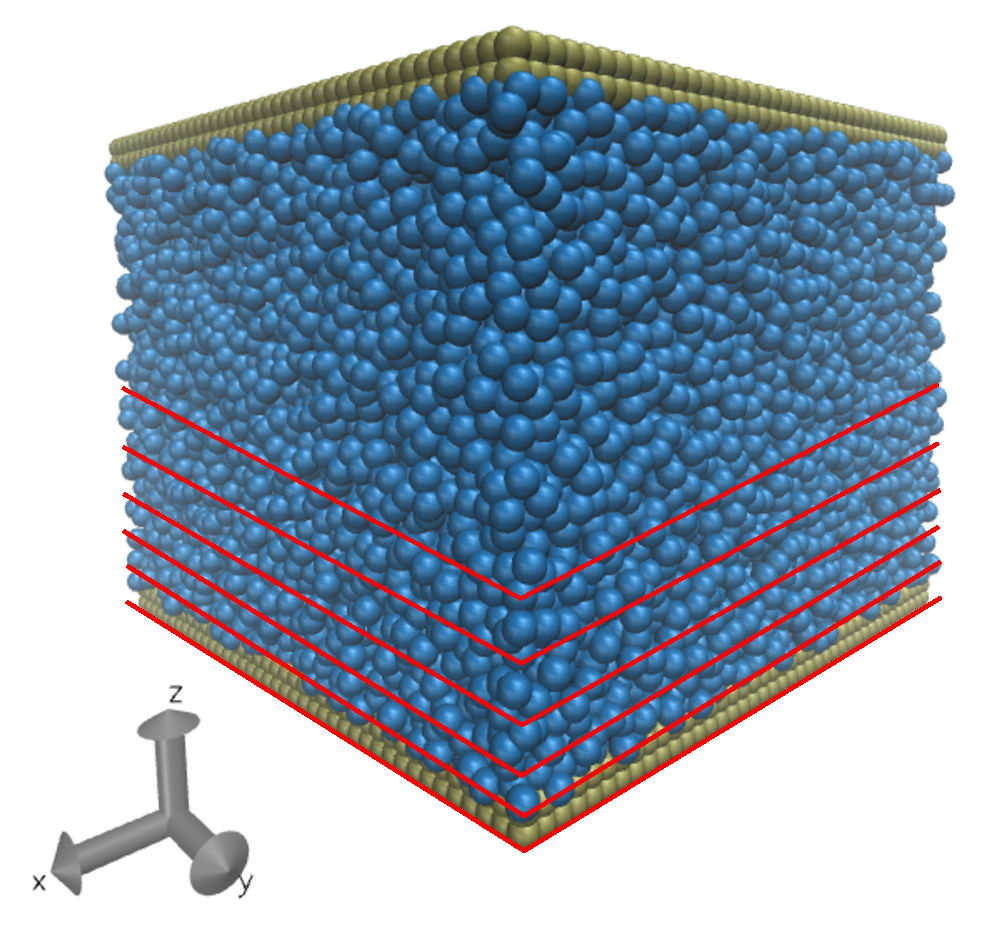
\includegraphics[scale=0.3]{system_nodes_walls}
    \caption[Walls box]{A visual representation of the MD simulation with a sketch of the binning used. In red are depicted the nodal planes used.}
    \label{fig:WallsBox}
\end{figure}
As in unconfined fluid simulations, we have checked that the correlations   $\llangle   \hat{\bf
  g}^1_\mu(t)\hat{\bf     g}^3_\nu\rrangle$,    $\llangle     \hat{\bf
  g}^1_\mu(t)\hat{\rho}_\nu\rrangle$     are    vanishingly     small,
corroborating  the predictions  of the  theory. Therefore,  as far  as
shear motion of  the fluid is concerned, a level  of description given
by the  parallel component  $\hat{\bf g}^1_\mu$ should  be sufficient.
We will consider elsewhere the  more general situation that allows one
to  study compression  of the  fluid in  the direction  normal to  the
walls.

The central quantity in this chapter, as well as in Chapter \ref{Chap:PBC}, is the equilibrium correlation matrix $C(t)$ of the CG variables given by
\begin{align}
  C(t)=\llangle \hat{g}(t) \hat{g}^T\rrangle
\end{align}
where  $T$  stands  for  transpose.   According  to  Mori  theory  the
correlation matrix decays in a linear way,
\begin{align}
 \frac{d}{dt}C(t)&= -\Lambda^*\esc C(t)
\label{InFull-C}
\end{align}
where  the  relaxation  matrix   $\Lambda^*$  is  a  constant  $N_{\rm
  bin}\times N_{\rm  bin}$ matrix. The relaxation  matrix subsumes all
  the transport coefficients  of the system. As shown  in Sec. \ref{Sec:MoriPBC},
the relaxation  matrix can  be decomposed  into a  non-local viscosity
contribution and non-local friction contributions, all defined through
Green-Kubo expressions,  suitably corrected  with the method  given in
Sec. \ref{Sec:CorrectedGK}.  As discussed in  Sec.  \ref{Sec:MarkovianAprox} a  Markovian equation
like (\ref{InFull-C}) is expected to hold only after a time $\tau$ has
elapsed. 

The Markovian relaxation equation (\ref{InFull-C}) predicts the following
evolution equation for correlation matrix
\begin{align}
  C^{\rm predict}(t)&=\exp\{-\Lambda^* (t-\tau)\}C(\tau)
\label{Cpredict}
\end{align}
where we  have introduced  the matrix  exponential through  its Taylor
series and have taken into account that Eq.  (\ref{InFull-C}) can only
be valid after  a time $\tau$. The elements of  the matrix exponential
do not  need to  decay as  exponential functions. As  we will  see, in
fact,  the decay  is  quasi-algebraic.   

In order to have an easier  identification of whether the evolution of
the  matrix  exponential  is   described  by  the  Markovian  equation
(\ref{InFull-C}) it  proves convenient to diagonalize  the correlation
matrix.   We introduce  eigenvalues  $\tilde{C}_\mu$ and  eigenvectors
$u_\mu$ in such a way that the  the correlation matrix is given by the
spectral decomposition
\begin{align}
  C(t)&=\sum_\mu^{N_{\rm bin}}\tilde{C}_\mu(t) u_\mu(t) \otimes u_\mu^T(t)
\label{spectral}
\end{align}
The unitary matrix $E(t)$ that  has as columns the eigenvectors allows
to diagonalize the correlation matrix, this is
\begin{align}
  E^{-1}(t)\esc C(t)\esc E(t)=\tilde{C}(t)
\label{diag}
\end{align}
where $\tilde{C}(t)={\rm Diag}[\tilde{C}_1(t),\cdots,\tilde{C}_{N_{\rm
    bin}}(t)]$ is a diagonal matrix  containing the eigenvalues in the
diagonal.   If  the  system  was traslation  invariant  in  the  $x^3$
dimension, the  matrix $E(t)$ would  be given by  the time-independent
discrete Fourier  transform, as discussed  in Chapter  \ref{Chap:PBC}.   In the
present problem where the solid walls break traslation invariance, the
unitary  matrix  $E(t)$ is  time  dependent.   As a  consequence,  the
diagonal matrix $\tilde{C}(t)$ evolves according to
\begin{align}
\frac{d}{dt}  \tilde{C}(t)&=-\tilde{\Lambda}^*\esc \tilde{C}(t)
  +\frac{d }{dt}(E^{-1}(t)) \esc C(t)\esc E(t)\nonumber\\
  &+E(t)\esc C(t)\esc \frac{d }{dt}E(t)  
\label{dc}
\end{align}
%\begin{align}
%\frac{d}{dt}  \tilde{C}(t)&=-\tilde{\Lambda}^*\esc \tilde{C}(t)
%+\frac{d }{dt}E(t) \esc E^{-1}(t) \esc \tilde{C}(t)\nonumber\\
%&+\tilde{C}(t)\esc \frac{d }{dt}E(t) \esc E^{-1}(t)  
%\label{dc}
%\end{align}
In Sec. \ref{Sec:ThinBins} we will show that the time dependence of the unitary  matrix is
very weak, $\dot{E}\simeq 0$, and allows one to approximate Eq. (\ref{dc}) as
\begin{align}
\frac{d}{dt}  \tilde{C}(t)&\simeq-\tilde{\Lambda}^*\esc \tilde{C}(t)
\label{Ctilde}
\end{align}
where,   consistently,  the   matrix  $\tilde{\Lambda}^*$   has  small
off-diagonal elements.   Therefore, we  arrive at the  conclusion that
the eigenvalues  $\tilde{c}_\mu(t)$ of  the correlation  matrix evolve
according to a single exponential
\begin{align}
  \tilde{C}_\mu(t)&=\exp\{-\tilde{\Lambda}_{\mu\mu} (t-\tau)\}  \tilde{C}_\mu(\tau)
\end{align}
where we have  taken into account that the  Markovian approximation is
valid only after the time $\tau$. This is one signature of the validity of the
Markovian equation (\ref{InFull-C}). Another signature of the validity is obtained from
each component of (\ref{Ctilde}) that shows that the function defined
as
\begin{align}
  \tilde{\Lambda}_{\mu}(t)&\equiv -\frac{1}{{\tilde{C}}_{\mu}(t)}\frac{d{\tilde{C}}_{\mu}}{dt}(t)
\label{LambdatRec}
\end{align}
should,  after  a time  $\tau$  reach  the  constant plateau  value  $
\tilde{\Lambda}_{\mu\mu}^*$.  Note  that the eigenvalues  should decay
exponentially  and,  therefore,  $  \tilde{\Lambda}_{\mu}(t)$  is  the
product  of an  exponentially decaying  function and  an exponentially
exploding function. This means that we need high quality statistics in
order  to have  sensible values  for $  \tilde{\Lambda}_{\mu}(t)$.  We
also realize that no matter how good our statistics is, we will always
encounter sufficiently large times where the exponential amplification
of statistical errors render  the function $ \tilde{\Lambda}_{\mu}(t)$
meaningless.

\section{MD simulations}
\label{Sec:SimWALLS}
The objetive of this section is to present the simulations we made to measure the matrix of correlations $C(t)$ in order to validate the Markoviam aproximation of a confined fluid. 
We follow the strategy presented in Chapter \ref{Sec:SimPBC}. Because the translational invariance is broken for confined fluids, it used, instead of the Fourier basis, the eigenvector basis of $C(t)$. 
In the first part of this section we deal with a sWe will deal with bines of diferent size, $\Delta z$.  
We deal with a system in which the space occupied by the fluid is exactly the same as in the case of an unconfined fluid. In the first part of this section the fluid region is divided in bins in which $Delta z$ is the same as the used in Chapter \ref{Chap:PBC}. In the second part, the size of the bins is doubled. 

\subsection{Simulation set up}
A system of particles interacting  with a LJ potential \ref{LJ}
truncated at $\sigma=2.5$ has been simulated with the open source code LAMMPS \cite{Plimpton1995}. The
box size  is $40\times40\times33$,  the number  of fluid  particles is
$N=28.175$ and  the time step  is $0.002$ in reduced  units.  Periodic
boundary conditions  (PBC) are assumed  in all directions.   Two solid
walls in the $xy$ plane confine the fluid as is shown in Fig. \ref{fig:WallsBox}.  The bottom wall is made of
two layers  of LJ  particles located  in a  simple cubic  lattice with
lattice spacing  $\sigma$. The top  wall is made  of two layers  of LJ
particles  in a  similar  cubic  lattice.  The  location  of the  four
crystalline planes  are $z=0,1,31,32$  in LJ units.   Due to  PBC, the
distance between  the layers of  solid particles which are  in contact
with   the  fluid   is  $3\sigma$   beyond  the   cutoff  of   the  LJ
potential. Therefore, the fluid particles occupy a space of $30\sigma$
and  do  not  interact  with  the  periodic  images  in  the  vertical
direction. Note that the space occupied by the fluid is equal to the case exposed in the previous chapter, in which the fluid is unconfined. 

After an equilibration of $10^5$ timesteps with a Langevin thermostate
to   produce  a   microstate  typical   from  a   thermodynamic  point
corresponding  to  $T=2,\rho=0.6$ in  reduced  units,  the system  is
evolved  under  NVE microcanonical  conditions  for  a further  $10^5$
timesteps.  After this equilibration  phase, production runs of $12\times 10^6$
time steps are launched and the transverse correlations are computed with the LAMMPS command \textit{ave/correlate} as it was explained in Sec. \ref{Sec:SimSetUpPBC}. 

\subsection{Thin bins with $\Delta z = 0.5\sigma$}
\label{Sec:ThinBins}
The $z$  axis is binned  in $66$ bins of  width of half  the molecular
size, $\Delta z=0.5\sigma$.  The  correlation matrix of the transverse
momentum of different bins is computed, requiring a total of $66\times
66$ time correlations  functions  in each  simulation.   
The support of  the correlation matrix  is extended only  up to a  time of
$t=1$ in reduced units, which  is sufficient to measure the relaxation
matrix.   A  few  selected  elements of  the  correlation  matrix  are
computed with a very long support of $t=30$ in reduced units, in order
to test the predictions of the theory at long times.

The time correlation  matrix is shown in  Fig.  \ref{fig:Ct-matrix-WALLS-66nodes} at
two different  times, $t=0$ and  $t=0.6$ in  reduced LJ units.   For the
covariance,  at $t=0$,  we  observe the  reminiscense  of the  density
layering near  the wall in the  form of peaks.  As  time proceeds, the
diagonal of  the correlation  widens and  decreases in  height.  Nodes
$\mu=0,1,64,65$ contain  no fluid, while  node $\mu=2,62$ have  a very
small  contribution  from  the  fluid but not negligible.  This means  that  out  of  the
$66\times66$ correlation matrix, we strip off a band of zeros, leaving
a matrix of $61\times61$ non-zero elements.

\begin{figure}[h!]
\centering
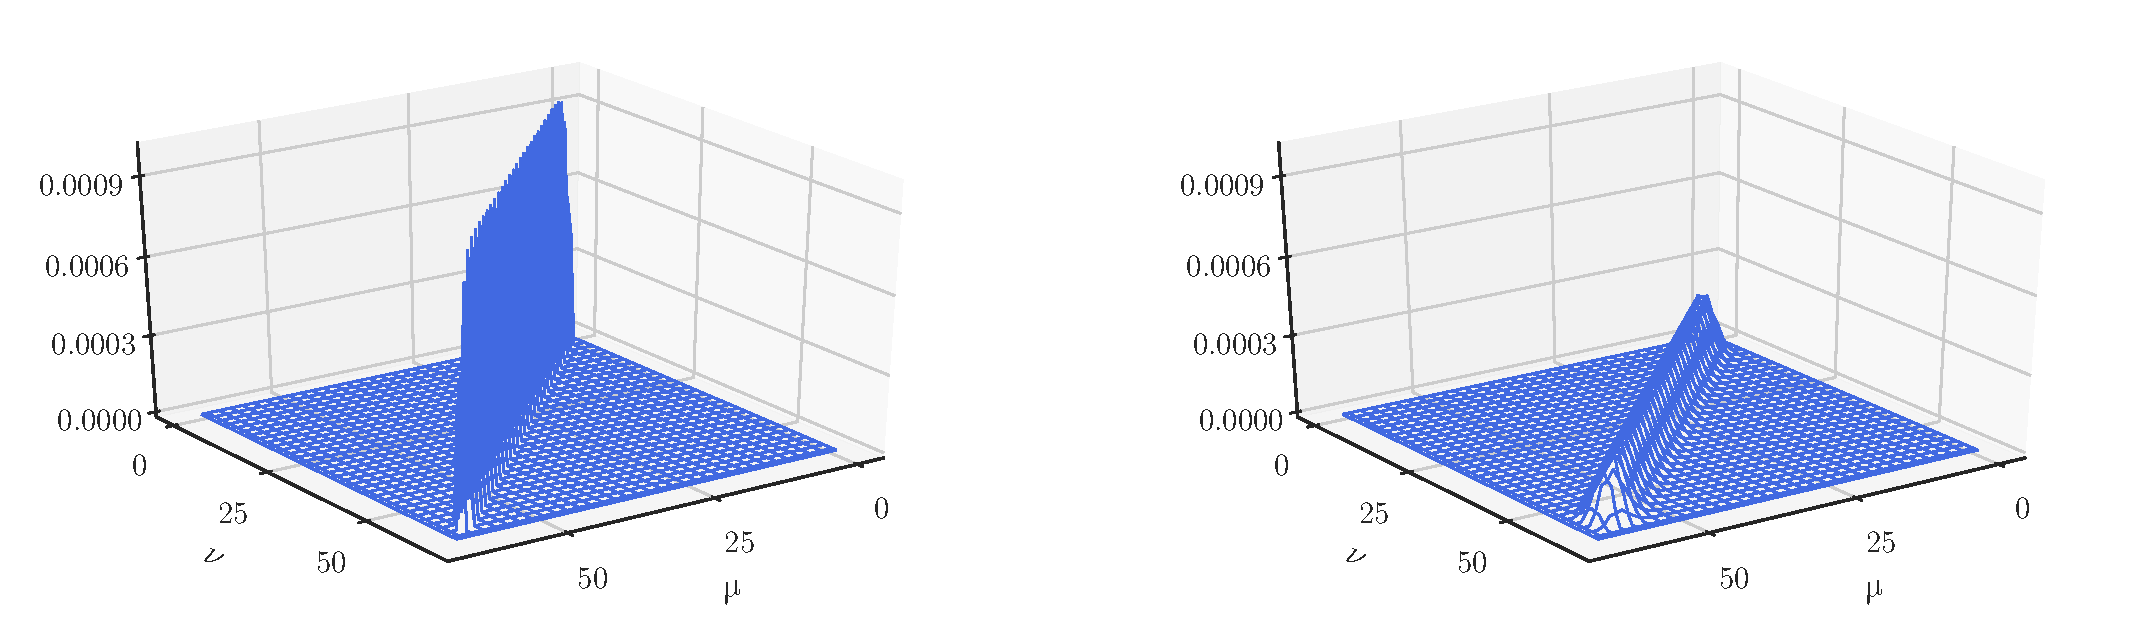
\includegraphics[scale=0.4]{Ct-matrix-WALLS-66nodes}
\caption[Correlation matrix $C(t)$ at $t=0$ and $t=0.6$ for confined fluid - 66 nodes.]{The   correlation    matrix   $C_{\mu\nu}(t)=\llangle
g_{\mu}(t)  g_\nu\rrangle$ for  $t=0$ (left) and $t=0.6$ (right).}
\label{fig:Ct-matrix-WALLS-66nodes}
\end{figure}

Next, we consider the time-dependent eigenvalues $\tilde{C}_\mu(t)$ of
the correlation matrix $C(t)$.  The eigenvector basis depends slightly
in time. We have checked that by  using the matrix $E(t)$ at the fixed
times  $t=0.15,0.30$  instead  of  the  time-dependent  matrix  $E(t)$  in
(\ref{diag}), the  correlation matrix $C(t)$  essentially diagonalizes
with  the same  eigenvalues,  therefore  validating the  approximation
(\ref{Ctilde}). i
This can be seen in Fig. \ref{fig:LambdatBasis-WALLS-66nodes}, 
where it plotted for clarity only $15$ elements of the diagonal of the matrix $\tilde{\Lambda}(t)$ in three different basis: 
$E(0.15)$, $E(0.30)$ and $E(t)$. 
\begin{figure}[h!]
  \centering
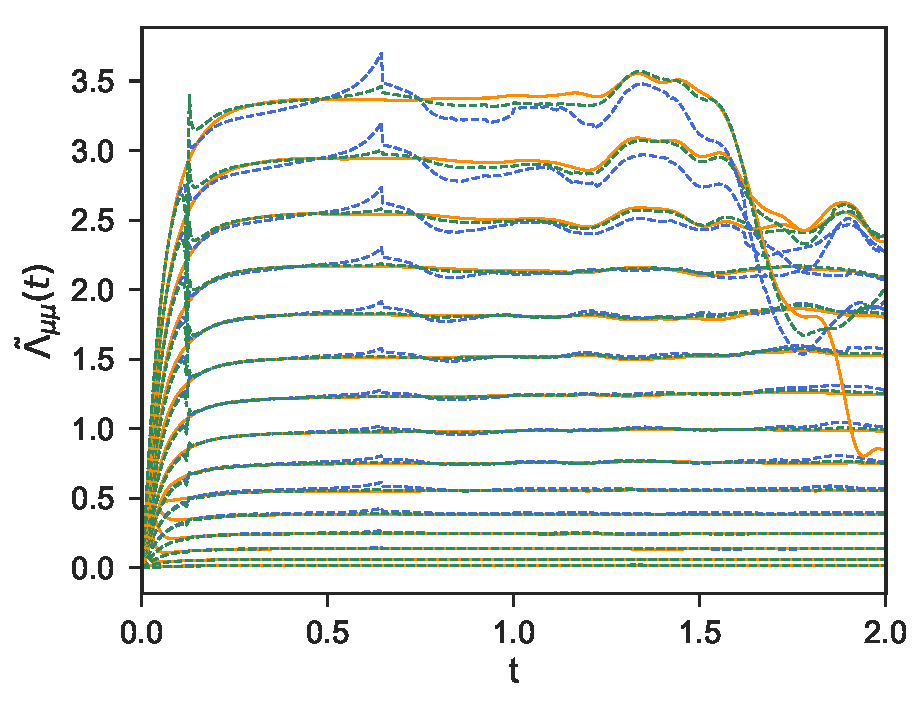
\includegraphics[scale=0.45]{LambdatBasis-WALLS-66nodes}
\caption[Diagonal elements  $\tilde{\Lambda}_{\mu\mu}(t)$ of $\Lambda(t)$ in three different basis - 66nodes.]{The  diagonal elements  $\tilde{\Lambda}_{\mu\mu}(t)$ of  the
  $\Lambda(t)$ in three basis:
$E(0.15)$ (dashed blue lines), $E(0.30)$ (dashed green lines) and $E(t)$ (solid orange lines). }
\label{fig:LambdatBasis-WALLS-66nodes}
\end{figure}


We plot in Fig.  \ref{fig:CtRec-WALLS-66nodes-exp}  all the 61 non-zero eigenvalues, in
descending  order,  as a  function  of  time. Statistical  errors  are
manifest in  the log-lin  plot, in spite  of the  overall high-quality
statistics. Also  clear from the log-lin  plot is the linear  decay of
the eigenvalues  beyond a certain  time, signaled by the  vertical red
line  located at  $\tau=0.2$.   Note that  at  $t=0$ the  correlation
matrix has zero  time derivative due to time  reversal invariance, and
this reflects in the parabolic,  not exponential, initial decay of the
eigenvalues \Note{Esto comentarlo también en PBC}.  In Fig.  \ref{fig:LambdatRec-WALLS-66nodes}  we show
the      function      $\tilde{\Lambda}_{\mu}(t)$      defined      in
(\ref{LambdatRec}). We only plot this  function for the data where the
eigenvalues   $\tilde{C}_{\mu}(t)>2\times10^{-5}$,    which   is   the
horizontal line plotted in the left panel in Fig.  \ref{fig:CtRec-WALLS-66nodes-exp}.  Below this value, which is
two  order  of  magnitude  smaller   than  the  value  at  $t=0$,  the
statistical errors  in the inverse  matrix blow up  exponentially, and
lead to an inverse that varies  erratically and is not reliable.  With
this cutoff,  a very  nice plateau  is observed  for the  lower modes,
reflecting the  exponential decay of  the eigenvalues as shown  in the
middle panel.

\begin{figure}[h!]
  \centering
  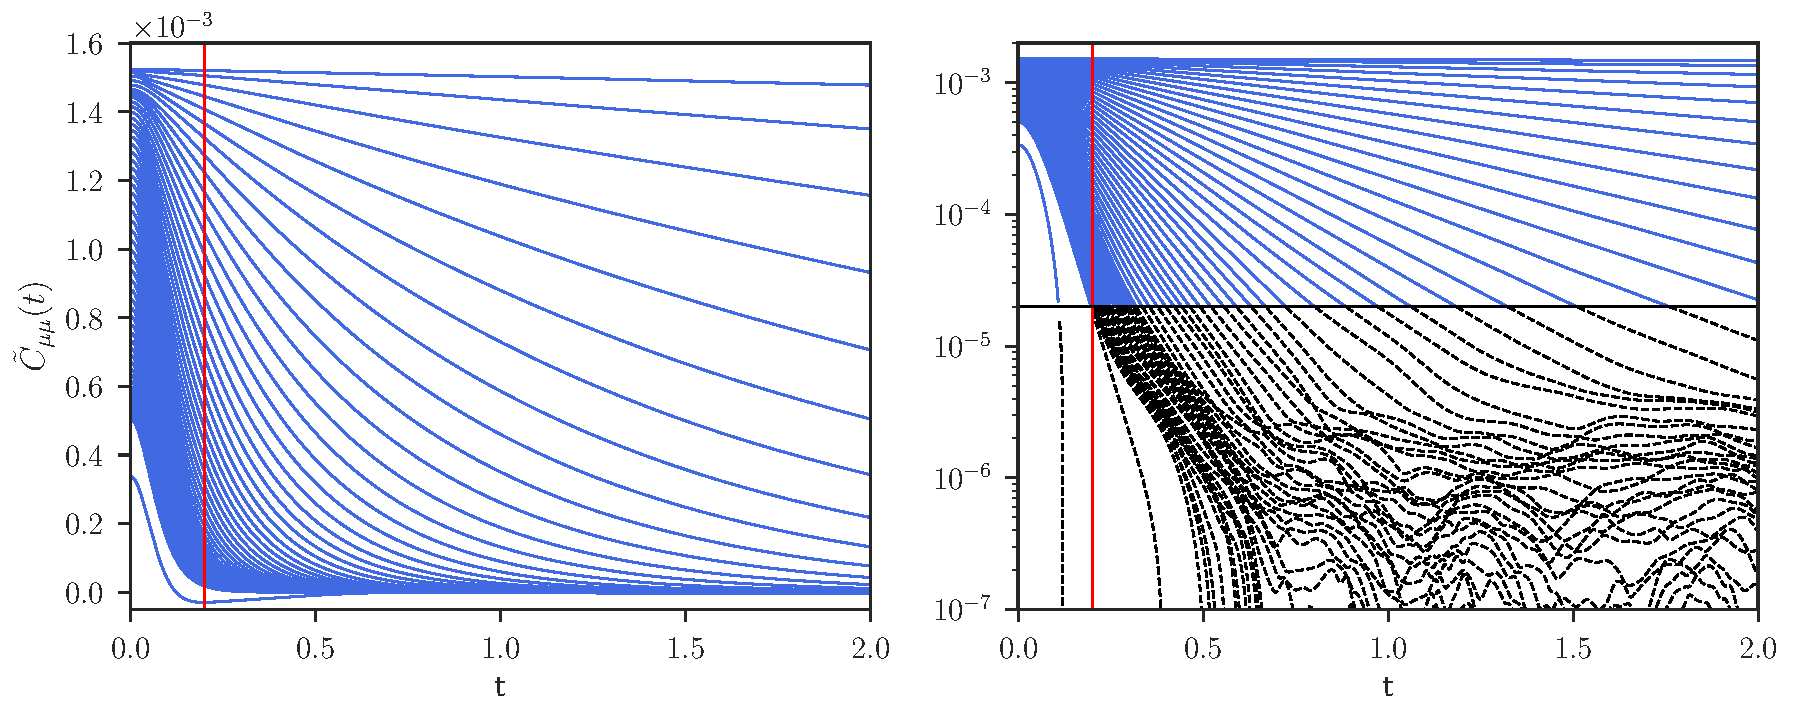
\includegraphics[scale=0.45]{CtRec-WALLS-66nodes-exp}
  \caption[Evolution of different eigenvalues $\tilde{C}_{\mu\nu}(t)$ for confined fluid - 66 nodes.]{
  The  evolution of  the different
  eigenvalues  $\tilde{C}_{\mu\mu}(t)$ of  the  correlation matrix  of
  momentum  as  a  function  of   time  in  a  lin-lin  plot  (left)
  and   log-lin   plot
  (right). Also  plotted are  a vertical line  at $t=\tau=0.2$  and a
  horizontal  line  at  the   value  $2\times10^{-5}$,  signaling  the
  threshold below which statistical errors give spurious results. }
\label{fig:CtRec-WALLS-66nodes-exp}
\end{figure}

\begin{figure}[h!]
  \centering
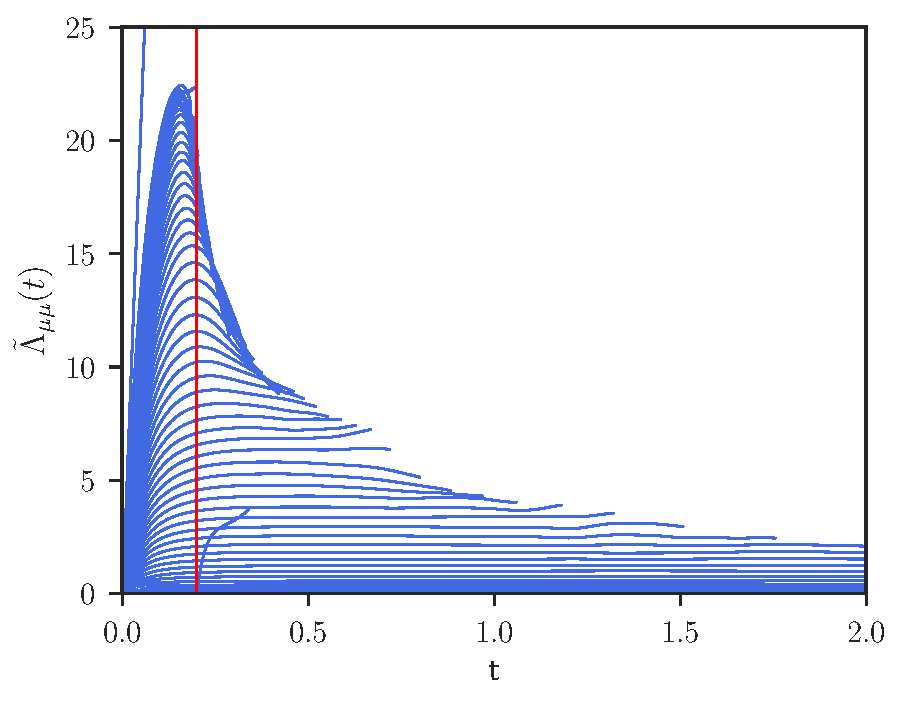
\includegraphics[scale=0.45]{LambdatRec-WALLS-66nodes}
\caption[Diagonal elements  $\tilde{\Lambda}_{\mu\mu}(t)$ of $\Lambda(t)$ in the reciprocal space - 66nodes.]{The  diagonal elements  $\tilde{\Lambda}_{\mu\mu}(t)$ of  the
  $\Lambda(t)$ in the reciprocal space defined in (\ref{}), as a
  function of $t$.}
\label{fig:LambdatRec-WALLS-66nodes}
\end{figure}

One  interesting feature  of the  spectrum of  the correlation  matrix
shown  in  Fig.  \ref{fig:CtRec-WALLS-66nodes-exp}  are  the  smallest two  eigenvalues
corresponding to $\mu=60,61$  that are clearly separated from the rest.
This eigenvalues are plotted in isolation for clarity in the left panel
of  Fig.  \ref{fig:EigenvaluesVectors-WALLS-66nodes}.   Note that  these eigenvalues  have a
distinct negative tail. This implies that  these modes do not decay in
an exponential way at all. The corresponding eigenvectors are shown in
the  right  panel of  Fig.   \ref{fig:EigenvaluesVectors-WALLS-66nodes}.   Note that  these
eigenvectors  are  localised  near   the  walls  and,  therefore,  the
contribution  of this  eigenvectors  into  the spectral  decomposition
(\ref{spectral}) boils  down to  a sort of  bounce-back effect  of the
fluid in the direction parallel to the walls.

\begin{figure}[h!]
  \centering
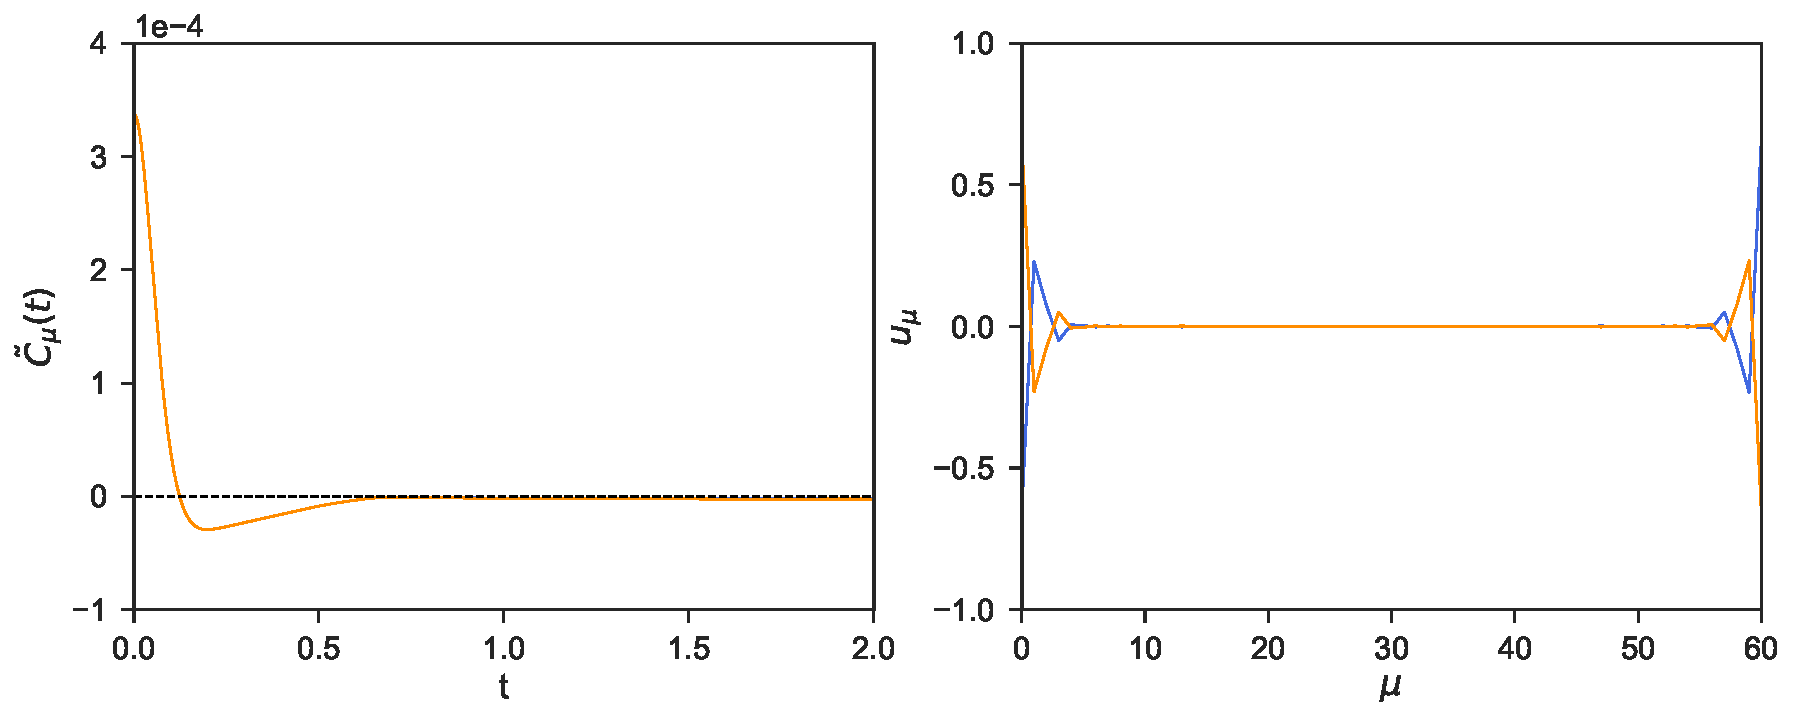
\includegraphics[scale=0.45]{EigenvaluesVectors-WALLS-66nodes}
\caption[Eigenvalues and eigenvectors near the walls for 66 nodes.]{The eigenvalues $\tilde{C}_{\mu}(t)$ of the correlation matrix $C(t)$ for $\mu=59,60$ which are identical and superimpose (left) and the corresponding eigenvectors $u_{\mu}$ in blue and orange, respectively (right).}
\label{fig:EigenvaluesVectors-WALLS-66nodes}
\end{figure}

The fact  that there are  eigenvalues that decay in  a non-exponential
way indicates  that the dynamics  is non-Markovian, at least  near the
walls. The non-Markovian effects could  be small, however, as only one
eigenvalue  is clearly  non-exponential.  In  order to  appreciate the
actual effect  of this  non-Markovian contribution to  the correlation
matrix in real space, we define the relaxation matrix in Fourier space
as   $\tilde{\Lambda}^*=\tilde{\Lambda}(\tau)$  for   $\tau=0.2$.   As
appreciated in Fig.   \ref{fig:LambdatRec-WALLS-66nodes}, this time
$\tau$ seems to  be a compromise for the minimum  time at which almost
all the elements $\tilde{\Lambda}_\mu(t)$ have reached the plateau and
yet the statistical errors due to  the inverse of the eigenvalues have
not exploded.   From $\tilde{\Lambda}^*$  we construct  the relaxation
matrix $\Lambda^*$ in  real space and, from  Eq.  (\ref{Cpredict}), we
obtain the prediction $C^{\rm  predict}(t)$ of the correlation matrix.
We plot in Fig. \ref{fig:Predictions-WALLS-66nodes} the  comparison of the measured and the
predicted correlation matrix  for particular elements $C_{\mu\mu}(t)$
of the matrix  along the diagonal.  In particular,  we choose $\mu=33$
which is in the middle of the  channel and $\mu=2,3$ which are the two
bins closer to the walls that have already fluid in it (bins $\mu=0,1$
do not contain  fluid particles due to the presence  of the wall).  In
the  top  panel  of  Fig.   \ref{fig:Predictions-WALLS-66nodes} are  the  results  for  the
autocorrelation in the middle of  the channel. The inset is a zoom at short times. The right plot, in logscale,
has  a support  up  to  $t=30$. The  agreement  between predicted  and
measured correlations is excellent in  the middle of the channel.  The
middle  and  bottom  panels  in Fig.   \ref{fig:Predictions-WALLS-66nodes}  describing  the
comparison   near   the   solid   wall,   however,   show   noticeable
discrepancies.   Very close  to  the wall,  for  $\mu=2$ the  measured
correlation displays  a bump,  better noticed  in the  logscale plot,
that  probably  reflects  the   ``bounce-back''  contribution  of  the
eigenvalues  $\mu=59,60$ in  the correlation  matrix (\ref{spectral}).
The  measured  autocorrelation  remains positive,  though,  while  the
predicted correlation  becomes negative.  Therefore, we  conclude that
the measured relaxation  matrix $\Lambda^*$ does not  allow to predict
through (\ref{InFull-C})  the correct  momentum correlations  near the
wall.   This is  clear sign  that the  dynamics near  the wall  is not
Markovian.


\begin{figure}[h!]
  \centering
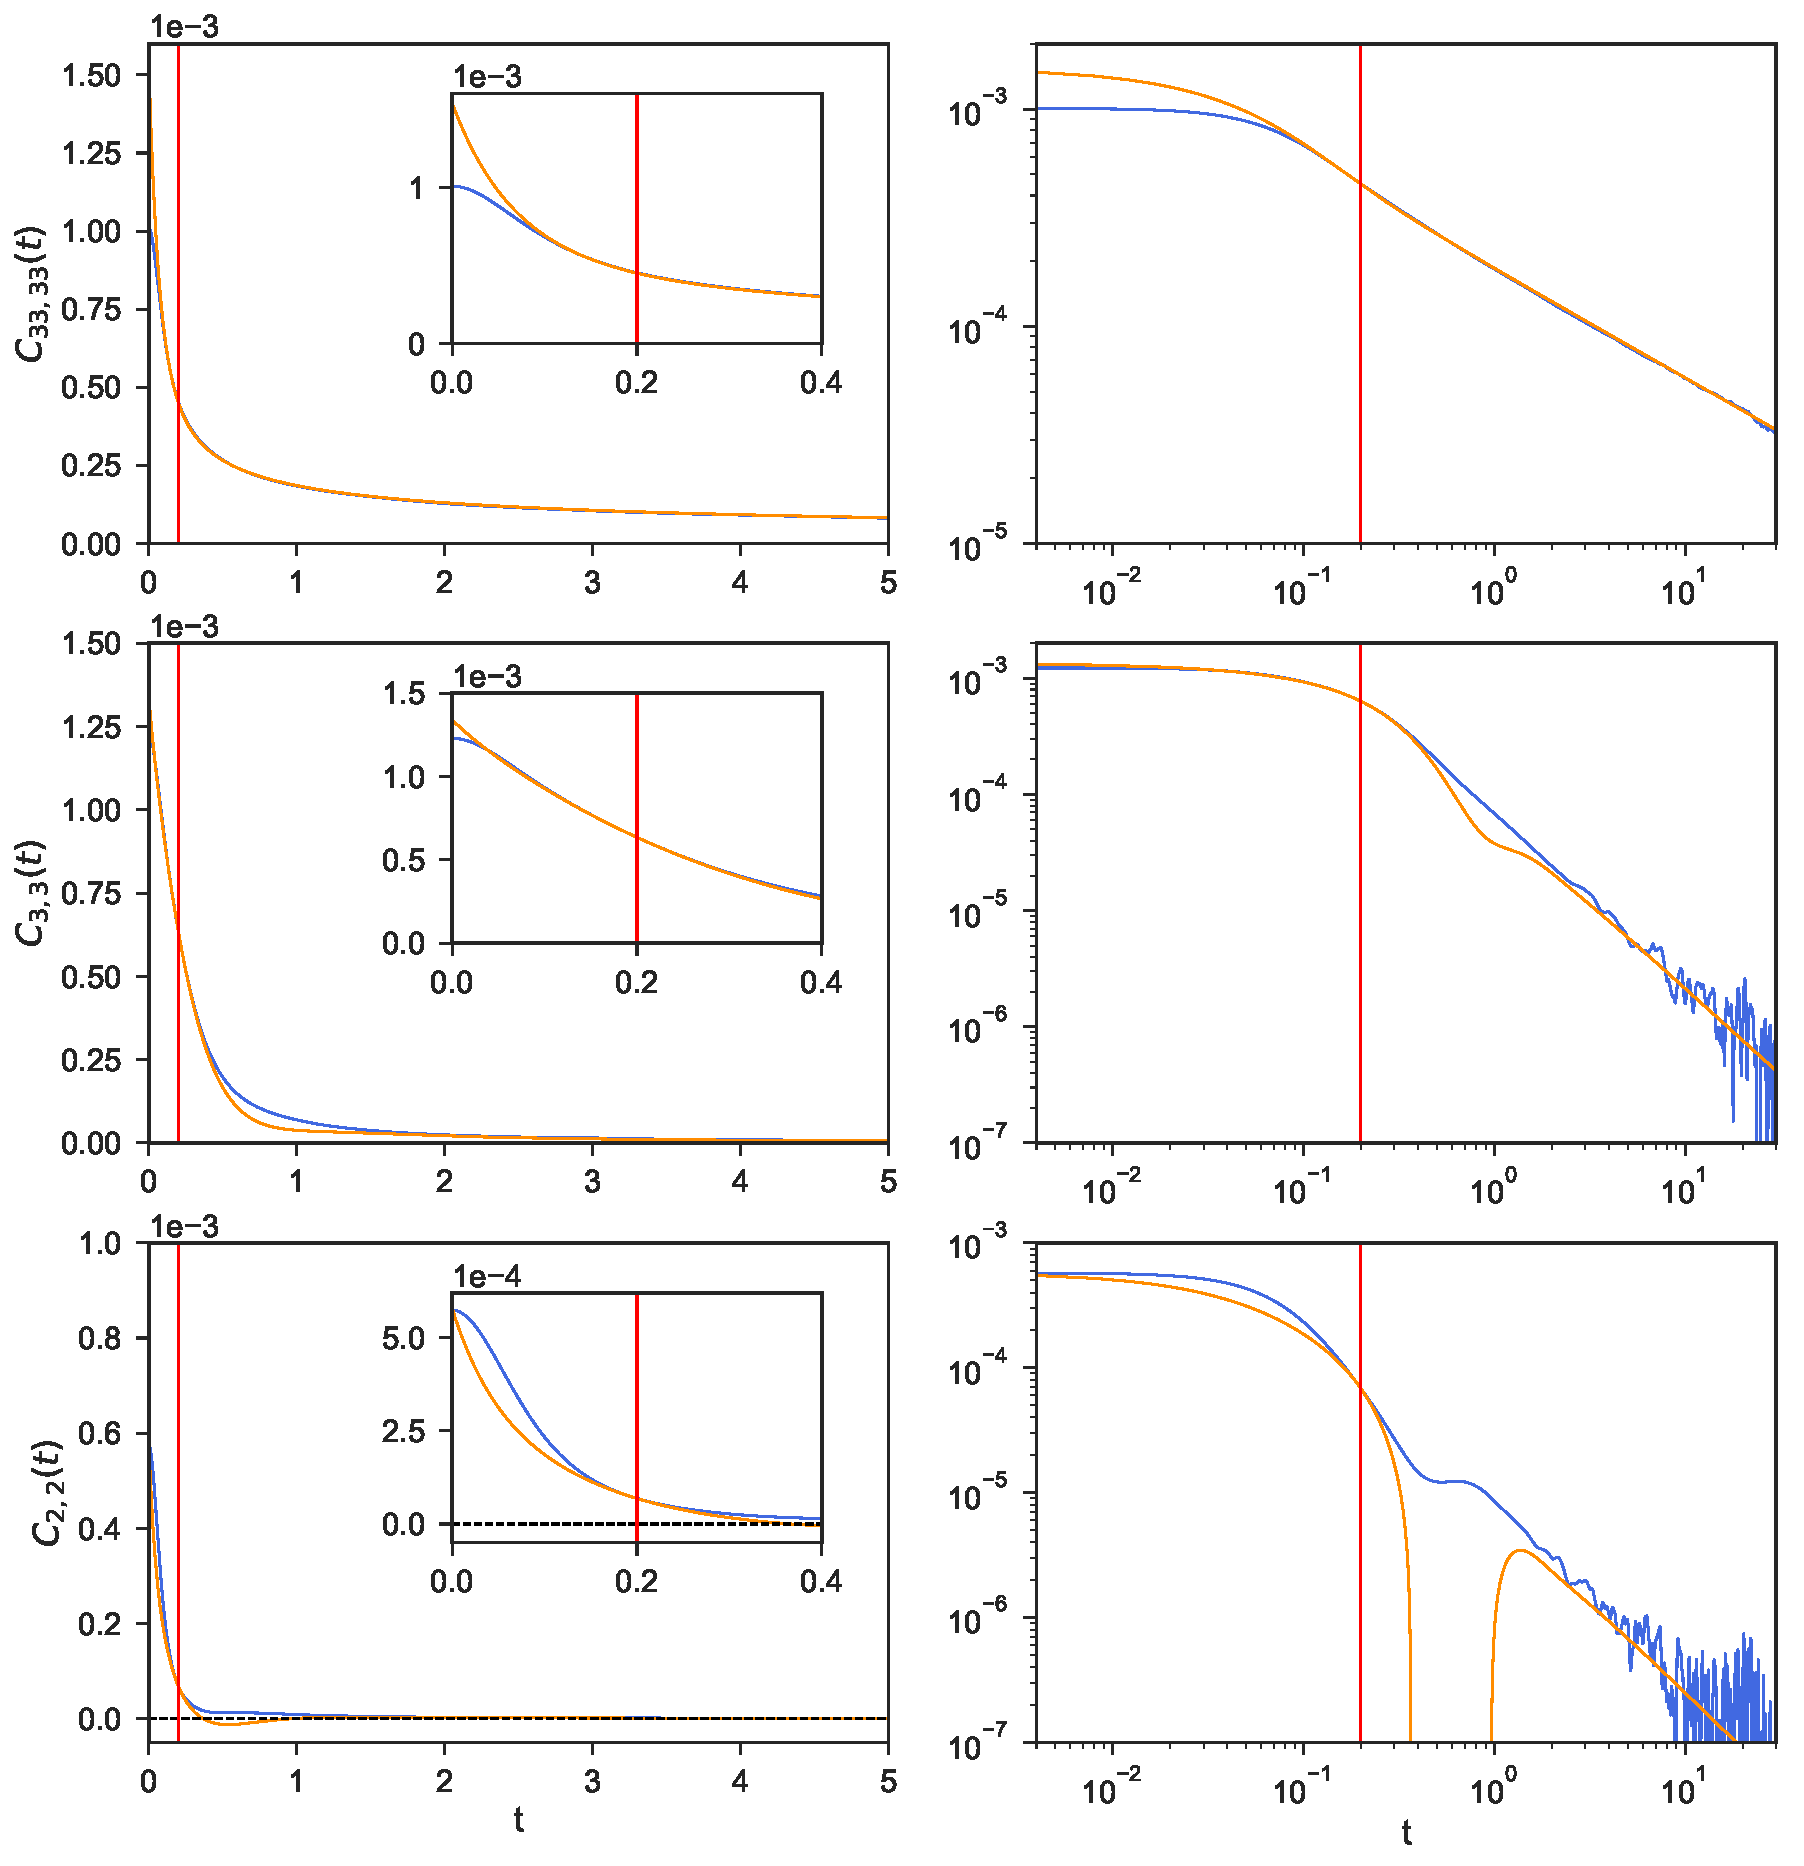
\includegraphics[scale=0.45]{Predictions-WALLS-66nodes}
\caption[Predicted autocorrelations of $C(t)$ for 66 nodes.]{The predicted (orange) and the measured (blue) values of the autocorrelation $C_{\mu\mu}(t)$ at different values of $\mu$ (top $\mu=33$, middle $\mu=3$ and bottom $\mu=2$). The predicted and measured correlations coincide by construction at $t=\tau=0.2$, where the vertical red line is. The inset shows a zoom at short times. The right panel is the same in logscale, where the correlations extends up to time $t=30$.}
\label{fig:Predictions-WALLS-66nodes}
\end{figure}

\subsection{Thick bins with $\Delta z = 2\sigma$}
In  order to  assess the  effect  of the  bin width  on the  Markovian
character of the  dynamics of the discrete momentum  variable, we have
conducted simulations  of the  same system but  with 33  nodal planes,
giving bins  of a  size $\Delta  z=\sigma$, and  with 17  nodal planes
giving a  bin width of  $\Delta z=2\sigma$.  The phenomenology  for 33
nodes  is very  similar to  the one  for 66  nodes.  
\Pendiente{In Fig. \ref{} we still observe negative eigenvalues and non-Markovian behaviour, although the effects are not so pronounced as for 66 nodes.}  
For 17 nodes the layering of the density field is not capture, as it showed in Fig. \ref{fig:DensityProfile-WALLS}


In  Fig.
\ref{fig:CtRec-WALLS-17nodes-exp}   (left   panel)   the   time   dependent   eigenvalues
$\tilde{C}_{\mu}(t)$  of  the  $17\times 17$  correlation  matrix  are
plotted as a function of time.  In the right panel, the logscale plot
shows a fairly linear decay, signaling exponential behaviour.  This is
more  clearly   seen  in   Fig. \ref{fig:LambdatRec-WALLS-17nodes},  where   the  function
$\tilde{\Lambda}_\mu(t)$  defined  in  (\ref{LambdatRec})  displays  a
plateau.   We select  the  plateau time  $\tau=0.3$  and measure  the
relaxation matrix $\Lambda^*$ as the Fourier transform of the diagonal
matrix  $\tilde{\Lambda}_{\mu}^*(\tau)$.   In  this way,  we  can  now
construct the  prediction (\ref{Cpredict}) for the  correlation matrix
$C(t)$ in real space. We  plot in Fig.  \ref{fig:Predictions-WALLS-17nodes} some selected
autocorrelations corresponding  to bins $\mu=7$  in the middle  of the
channel,  $\mu=4$ which  is  a  quarter distance  from  the wall,  and
$\mu=1$  the  first   bin  with  fluid  (bin  $\mu=0$   has  no  fluid
contribution).   We   observe  an  excellent  agreement   between  the
predicted and measured correlations.  This agreement is also very good
for the  cross-correlations, as shown in  Fig. \ref{fig:PredictionsCross-WALLS-17nodes}. Note
that the  cross-correlation $C_{8,7}(t)$ is non-zero  at $t=0$ because
the momentum at a  given node is defined in terms  of a finite element
basis  function.  For neighbouring  nodes,  the  finite element  basis
overlap  and this  gives  rise  to the  non-zero  value  of the  cross
correlation.  On  the other  hand, for nodes  separated by  two units,
where the finite elements no  longer overlap, the cross correlation at
$t=0$ vanishes, as it is clear for $C_{3,5}(t)$.



\begin{figure}[h!]
  \centering
  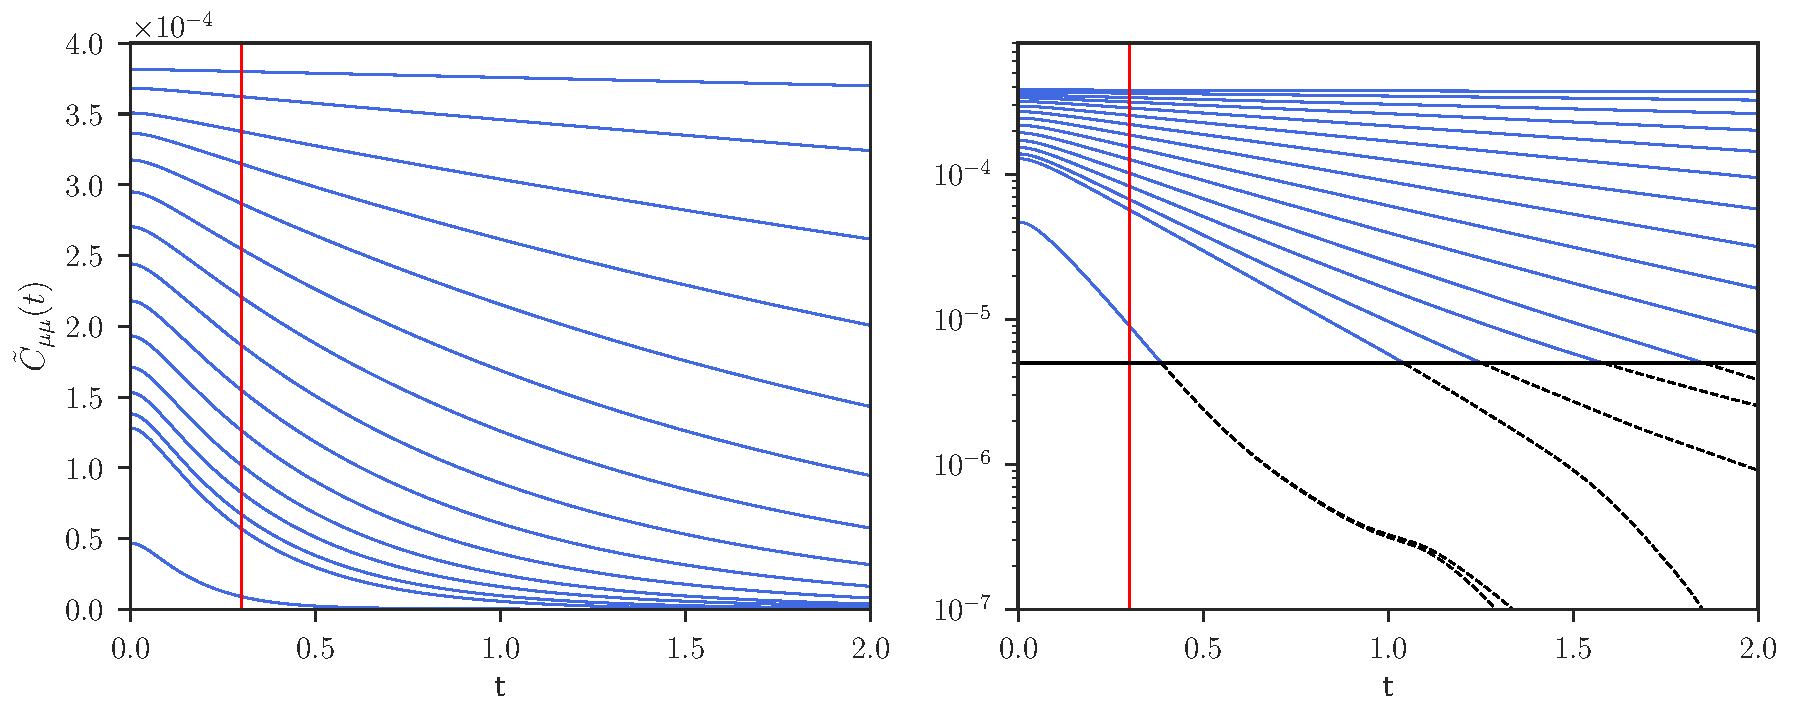
\includegraphics[scale=0.45]{CtRec-WALLS-17nodes-exp}
  \caption[Evolution of different eigenvalues $\tilde{C}_{\mu\nu}(t)$ for confined fluid - 17 nodes.]{
  The  evolution of  the different
  eigenvalues  $\tilde{C}_{\mu\mu}(t)$ of  the  correlation matrix  of
  momentum  as  a  function  of   time  in  a  lin-lin  plot  (left)
  and   log-lin   plot
  (right). Also  plotted are  a vertical line  at $t=\tau=0.3$  and a
  horizontal  line  at  the   value  $5\times10^{-6}$,  signaling  the
  threshold below which statistical errors give spurious results. }
\label{fig:CtRec-WALLS-17nodes-exp}
\end{figure}

\begin{figure}[h!]
  \centering
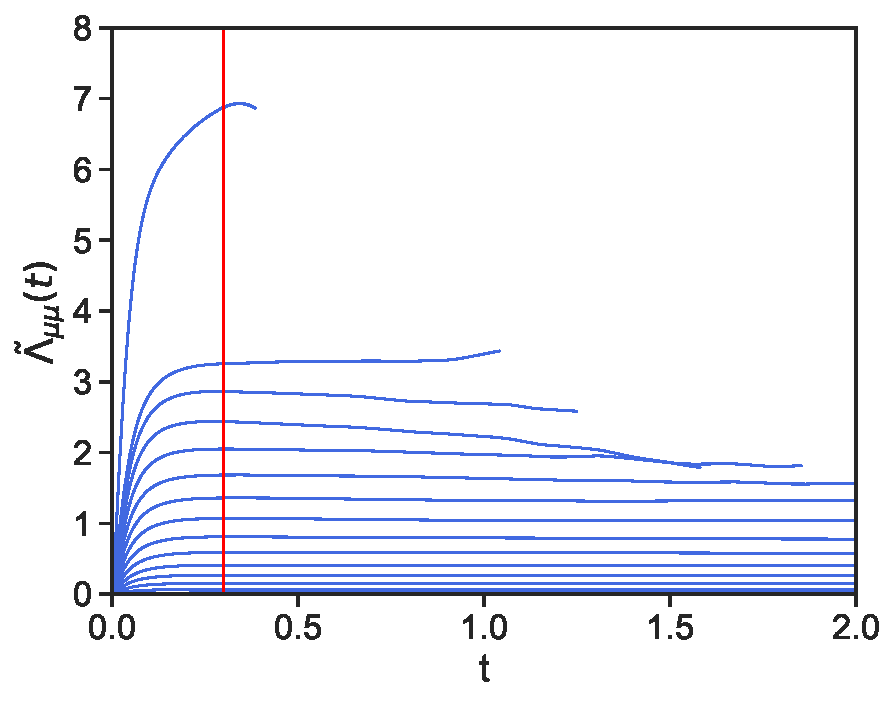
\includegraphics[scale=0.45]{LambdatRec-WALLS-17nodes}
\caption[Diagonal elements  $\tilde{\Lambda}_{\mu\mu}(t)$ of $\Lambda(t)$ in the reciprocal space - 17nodes.]{The  diagonal elements  $\tilde{\Lambda}_{\mu\mu}(t)$ of  the
  $\Lambda(t)$ in the reciprocal space defined in (\ref{}), as a
  function of $t$.}
\label{fig:LambdatRec-WALLS-17nodes}
\end{figure}

\begin{figure}[h!]
  \centering
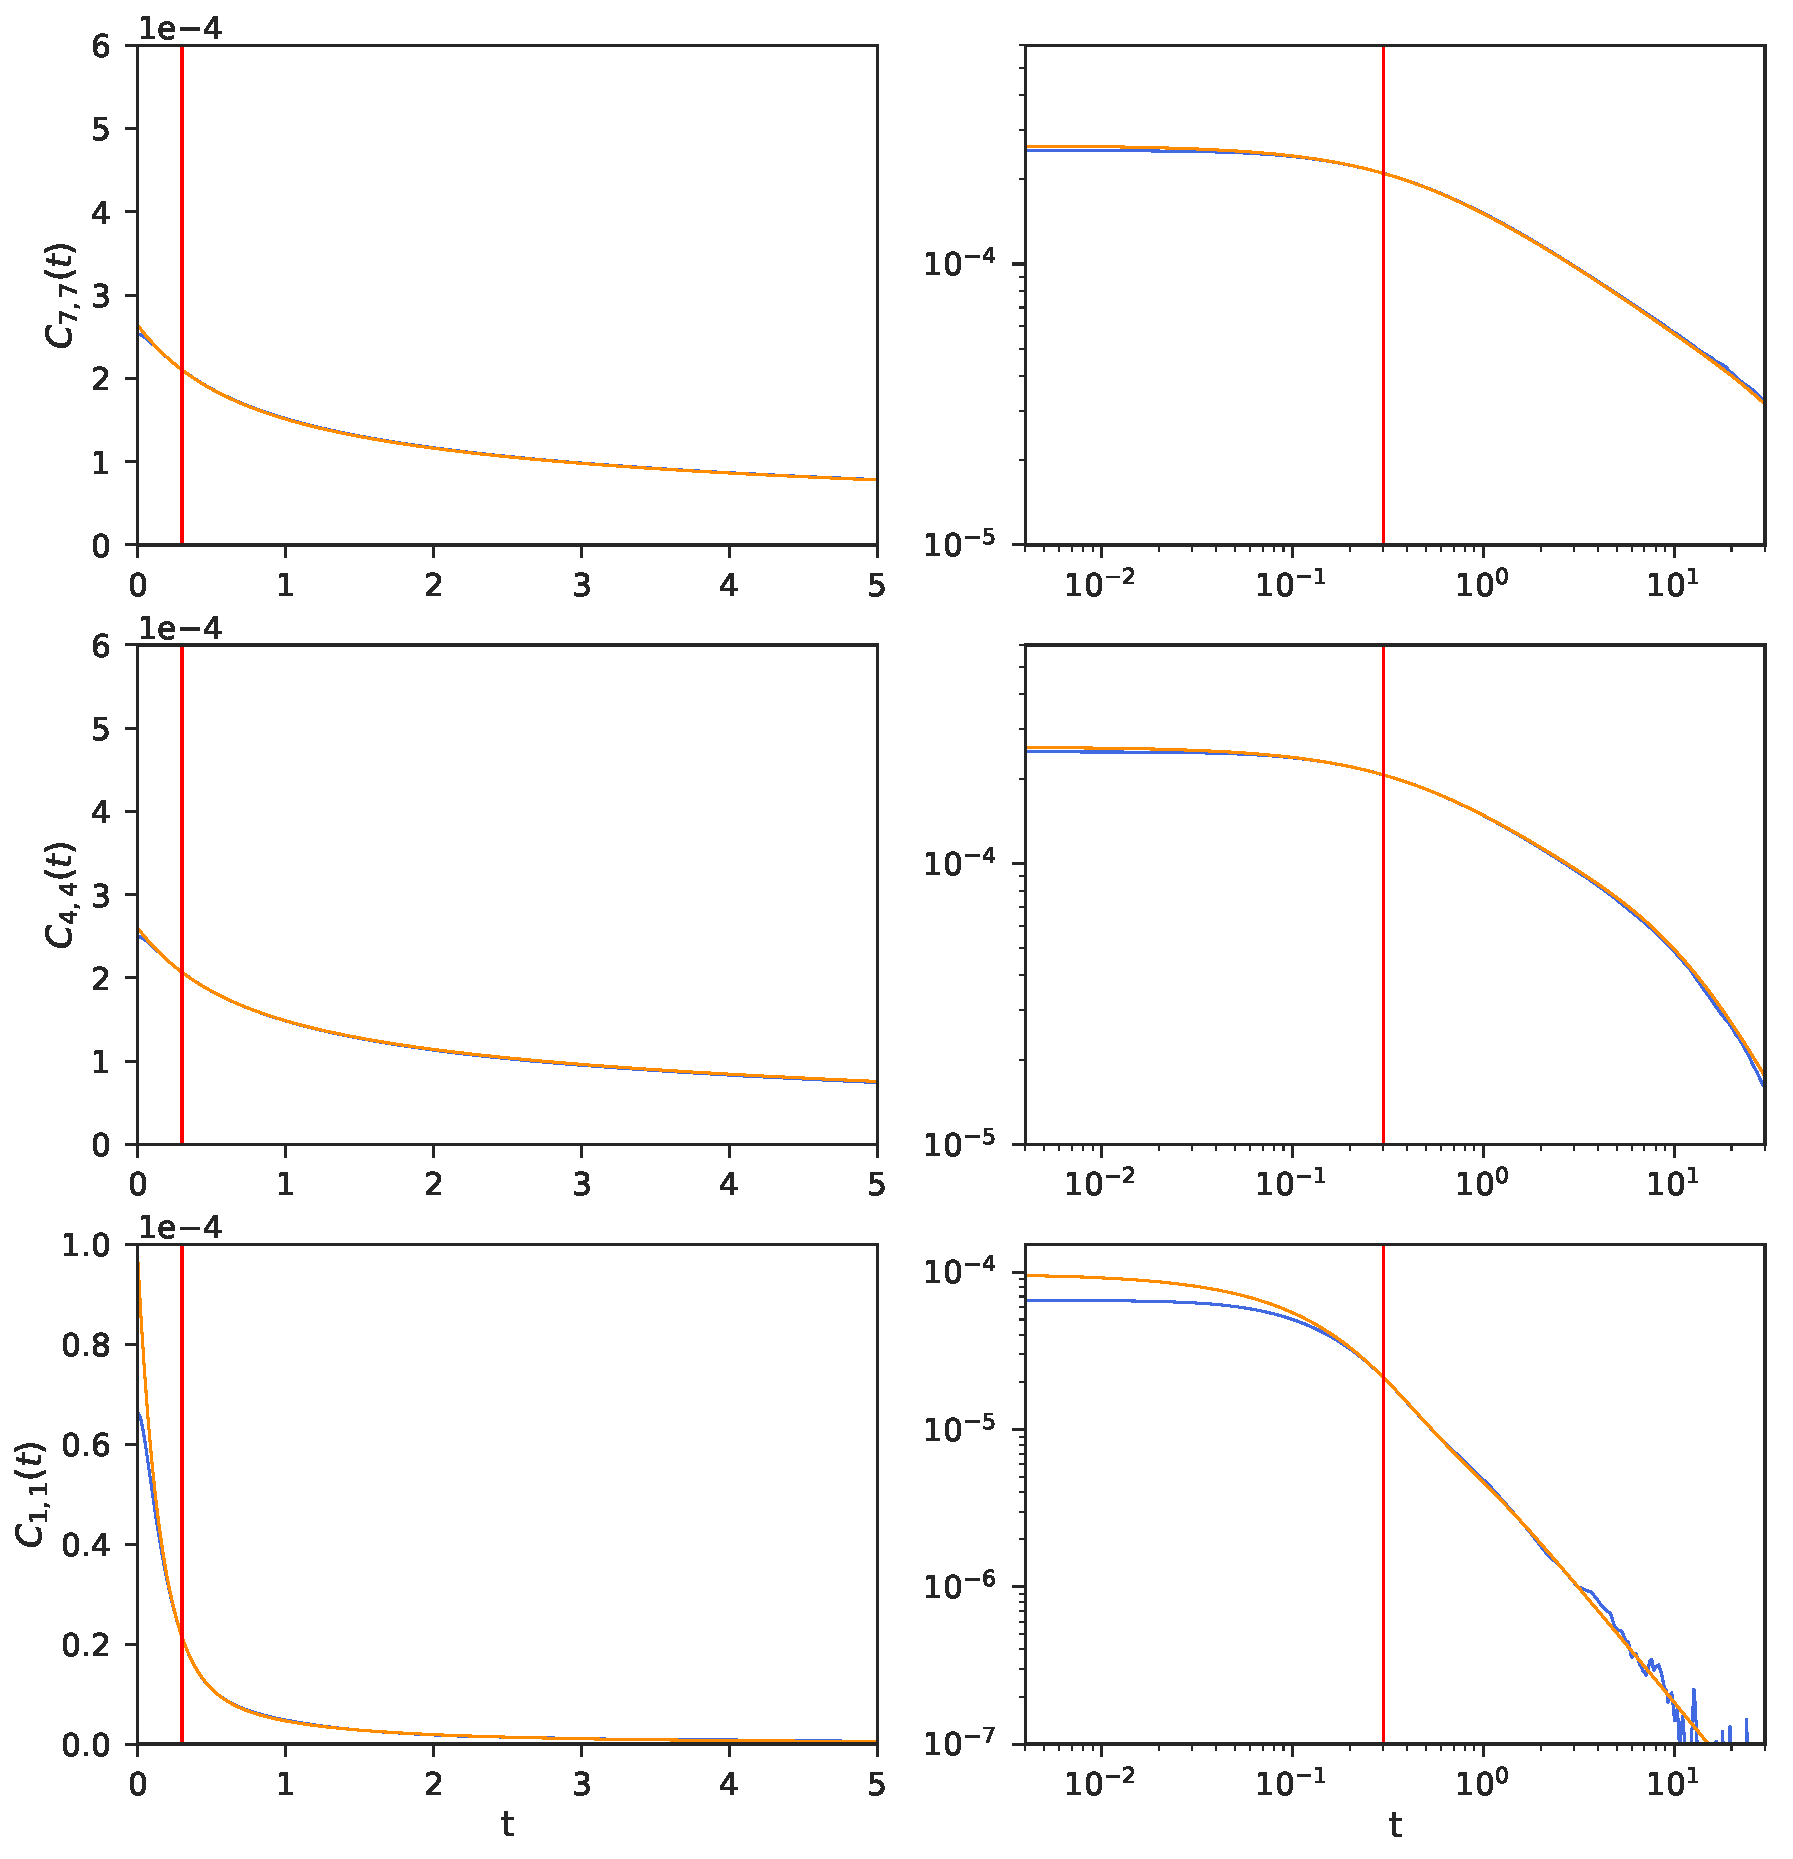
\includegraphics[scale=0.45]{Predictions-WALLS-17nodes}
\caption[Predicted autocorrelations of $C(t)$ for 17 nodes.] {Autocorrelations $C_{\mu\mu}(t)$  for different  bins $\mu=1$
  (bottom),  $\mu=4$  (middle),  and  $\mu=7$ (top).  The  right panel  is  in 
  logscale with a support up to $t=30$. The red line is plot at $t=0.3$}
\label{fig:Predictions-WALLS-17nodes}
\end{figure}


\begin{figure}[h!]
  \centering
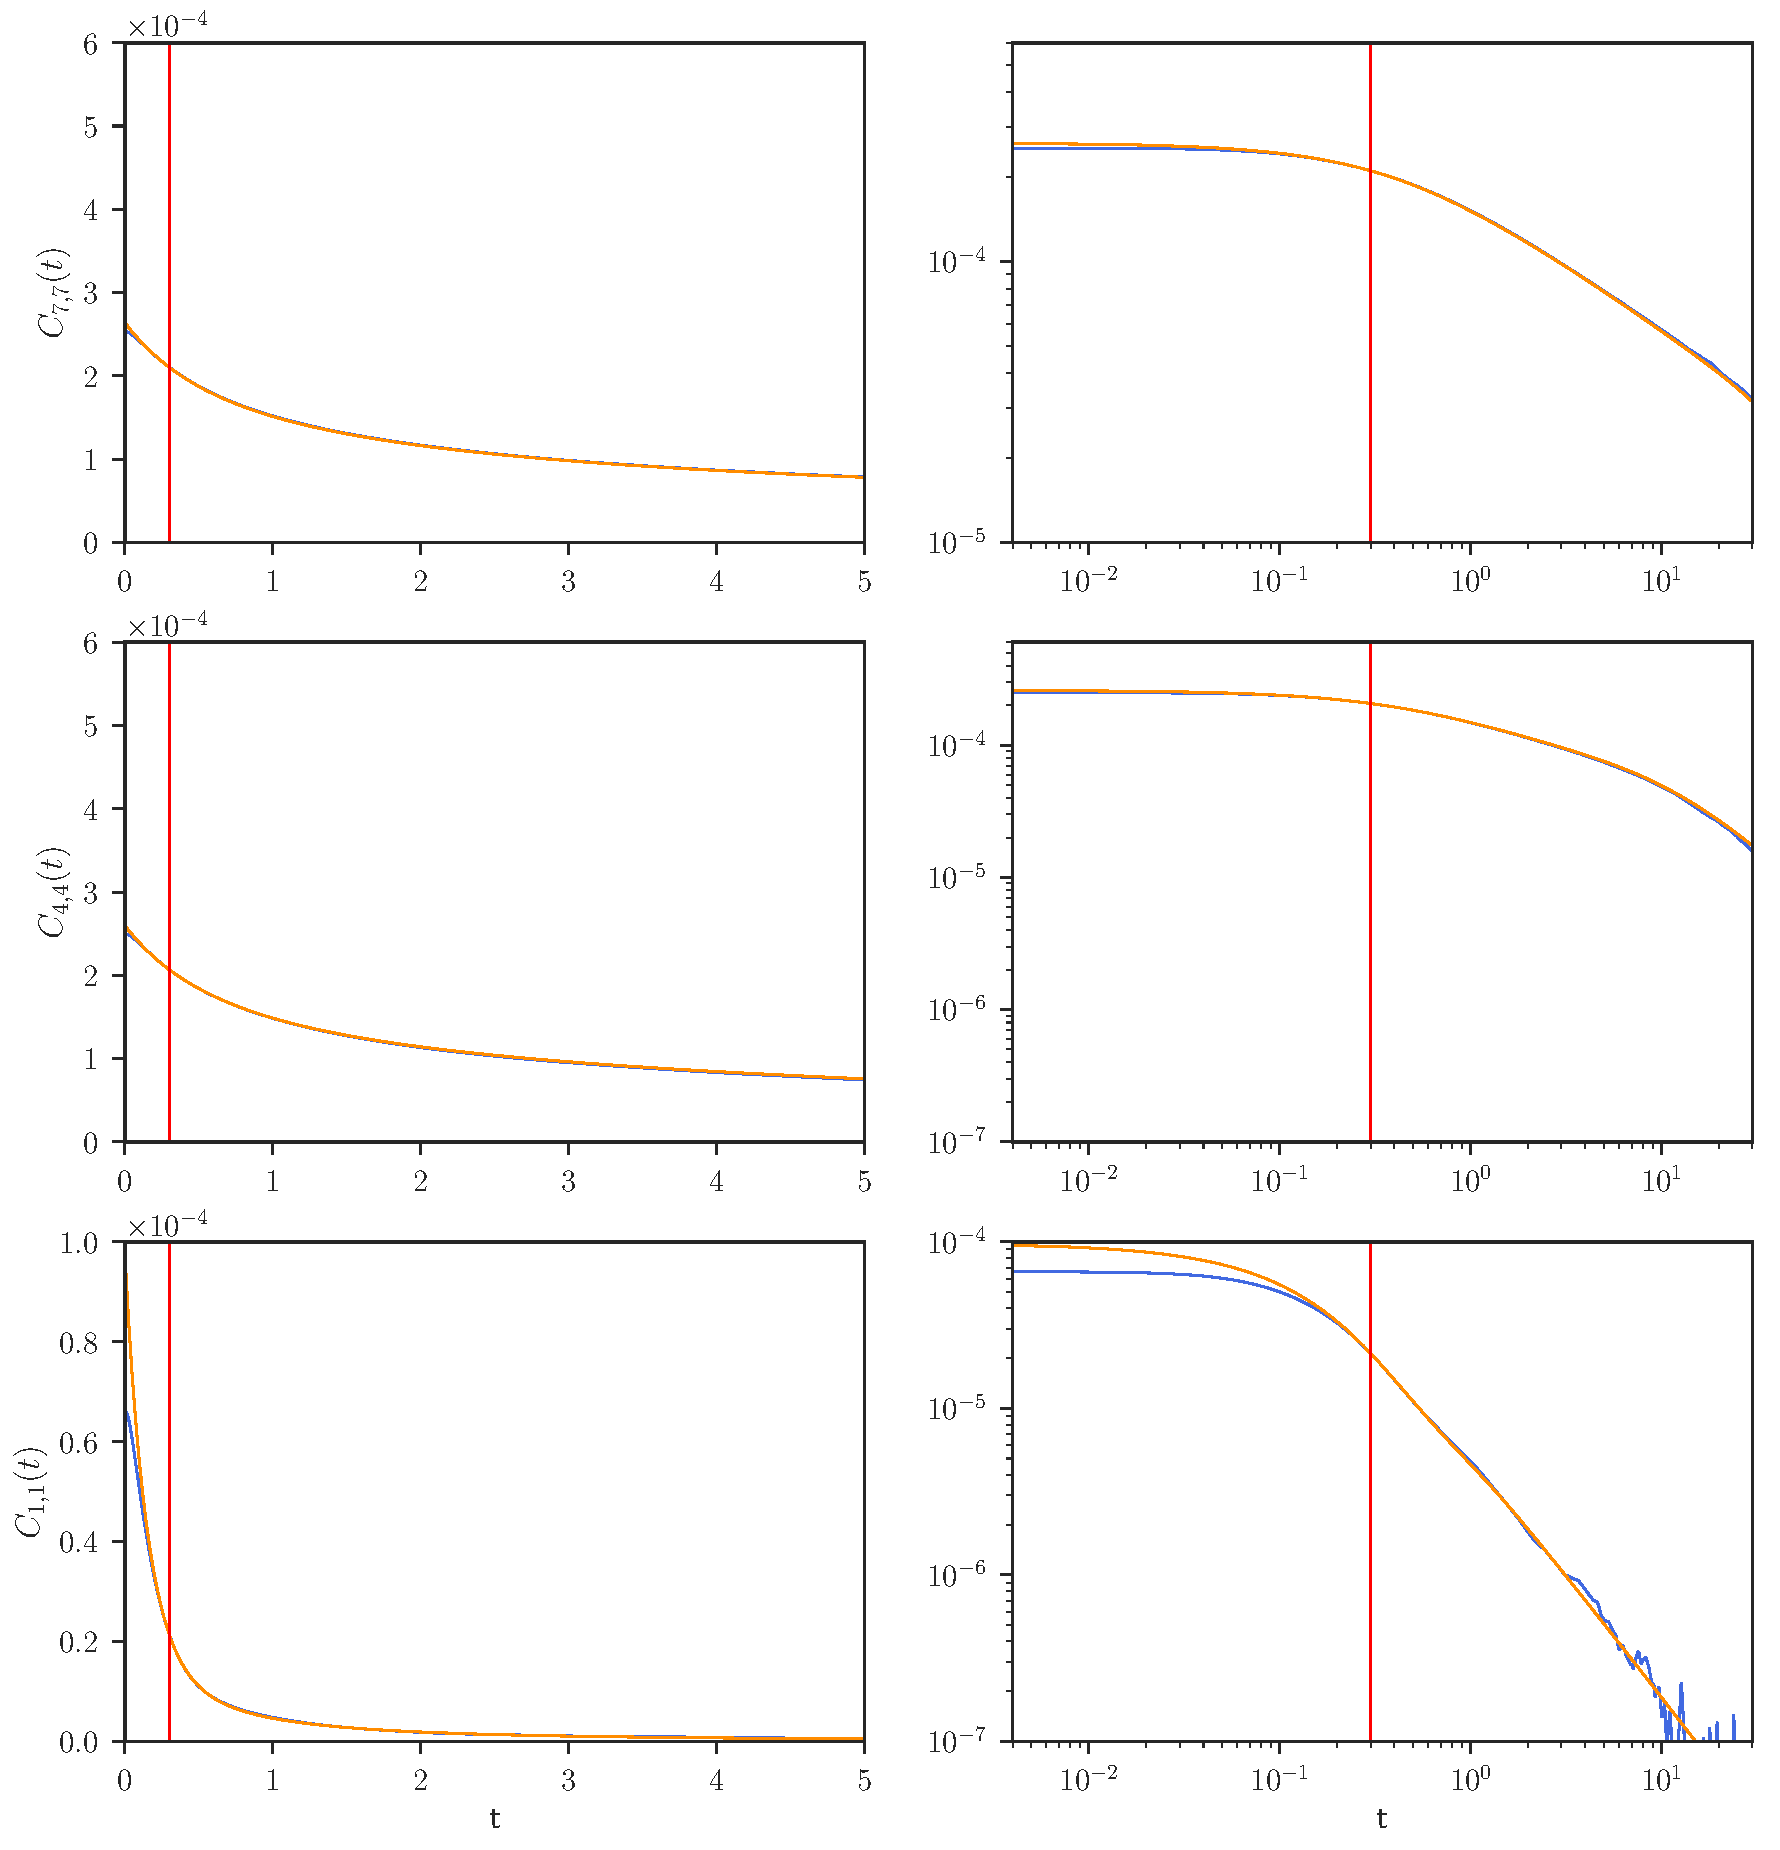
\includegraphics[scale=0.45]{PredictionsCross-WALLS-17nodes}
\caption[Predicted crosscorrelations of $C(t)$ for 17 nodes.]{The crosscorrelations between nodes $\mu=3,\nu=5$ (bottom) and  $\mu=8,\nu=7$ (top). The right pael is in logscale, and the red line is plot at $t=30$.}
\label{fig:PredictionsCross-WALLS-17nodes}
\end{figure}

\section{Conclusions}
In this chapter we have considered  the discrete hydrodynamics of  a LJ
fluid  confined  between   two  rigid  parallel  walls   of  fixed  LJ
particles. We  measure the correlation  matrix $C(t)$ of  component of
the discrete momentum density which is  parallel to the walls.  According
to  Mori theory,  under the  Markovian approximation  this correlation
should decay  in a  matrix exponential form  with a  relaxation matrix
$\Lambda^*$ that  can be  obtained from the  plateau region  where the
decay  of  $C(t)$  is  exponential.  By  looking  at  the  eigenvalues
$\tilde{C}_\mu(t)$  of the  correlation  matrix,  the Markov  property
translates into an  exponential decay of all the  eigenvalues. We have
observed that  for bins  smaller than  molecular dimensions  $\Delta z
\leq  \sigma$,  where  $\sigma$  is  the  LJ  diameter,  some  of  the
eigenvalues do  not decay  as exponential  and become  negative.  Even
though we can estimate a relaxation matrix from the plateau that gives
good predictions away  from the wall, the correlations  near the walls
are poorly described by the Markovian theory.

When we  increase the  size of  the bins, up  to $\Delta  z=2\sigma$, a
Markovian theory gives excellent results, where all the eigenvalues of
the   correlation  function   decay   exponentially,  a   well-defined
relaxation  matrix  $\Lambda^*$ can  be  measured,  and the  resulting
predictions  with  this  relaxation  matrix reproduce  very  well  the
measured correlation matrix.

The present chapter follows the  methodology of Chapter \ref{Chap:PBC}  where we
have  discussed  the  correlation  matrix  of  the  discrete  momentum
parallel to  the bins in  an \textit{unconfined} system  with periodic
boundary  conditions.  We  have  observed there  that the  correlation
matrix for the discrete momentum defined  in thin bins of size $\Delta
z= 0.5\sigma$ behaves in a Markovian way. Of course, this behaviour is
observed  only beyond  certain time  $\tau$, as  observed also  in the
present chapter.  It is clear that the breaking of the Markov assumption
for thin bins is due to the presence of the walls, which is consistent
with  the   observation  that  the  eigenvectors   of  the  non-Markov
eigenvalues are different  from zero only near the  walls. The physics
behind this non-Markov  behaviour for thin bins is  not entirely clear
but  we note  that for  thin bins,  we are  resolving scales  that are
comparable   to   the   ``roughness''    of   the   lattice   of   the
walls. Therefore, it is plausible that the bump in the autocorrelation
of the  bin close  to the lattice  shown in the  bottom panel  of Fig.
\ref{fig:Predictions-WALLS-66nodes} is  due to a  ``caging effect'' of the  fluid particles 
due to the lattice. Such a caging would be undetectable for much wider
bins, as it appears to be the case.

In  the  present  paper,  we  have  only  discussed  the  dynamics  of
transverse momentum.   With the same  methodology, we can  discuss the
coupled  dynamics of  the  density  and the  normal  component of  the
momentum.   It is  not yet  clear to  us whether  the highly  resolved
hydrodynamics near  the wall, that  reproduce the density  layering as
shown in  Fig.  \ref{fig:DensityProfile-WALLS} is  Markovian or  not. In any  case, we
expect that the study of perpendicular sound waves confined in between
parallel walls deserves further study.

\begin{figure}[h!]
  \centering
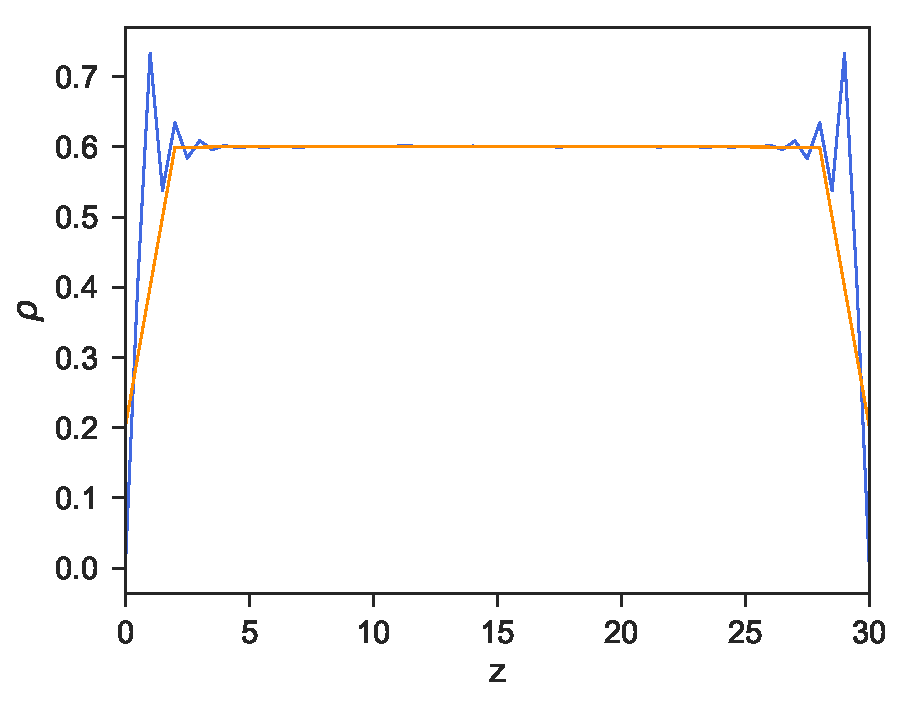
\includegraphics[scale=0.45]{DensityProfile-WALLS}
\caption[Fluid density profile for 66 and 17 nodes.]{The equilibrium average discrete density for thin bins (blue) and thick bins (orange). The thick bins do not capture the layering of the density field.}
\label{fig:DensityProfile-WALLS}
\end{figure}

The  fact that  hydrodynamics near  walls is  non-Markovian at  highly
resolved  scales  has a  number  of  implications. For example, in Chapter \ref{Chap:Theory} the coarse delta function introduced in the hydrodynamic fields can not be a Dirac delta functions as we presented in \cite{Camargo2018}. 
\Note{Esto no hará falta añadirlo porque voy a cambiar el capítulo 2. For  example,  the
continuum theory  described in Chapter \ref{Chap:Theory} can  only make
sense if the hydrodynamic fields are  defined not with the Dirac delta
function, but  rather with  coarse delta  functions with  an intrinsic
length  scale  larger than  molecular  dimensions  as, for  example  a
normalized Gaussian  of width  $\sigma$.  As  a consequence,  the free
energy functional  that emerges from  such a coarsely  defined density
field  is not  directly  given by  the usual  free  energy density  in
Equilibrium  Density Functional  Theory, which  is, in  fact, the  one
particle distribution function.  In fact,  a local model for the free energy 
is expected for  the former. The resulting free  energy functional for
coarsely  defined density  cannot  resolve the  density layering  near
walls.   It is  obvious now  that in  order to  describe the  resolved
dynamics of the density layering  near a wall requires a non-Markovian
theory  or,   alternatively,  a   Markovian  theory   with  additional
non-hydrodynamic variables.  Perhaps the  stress tensor is a candidate
to capture the apparent viscoelasticity of the density layering.}

Note   that   it    only   make   sense   to    speak   of   transport
\textit{coefficients} (or matrices of) in theories that are Markovian,
otherwise  one  needs   transport  \textit{memory  kernels}.   Another
implication of  non-Markovianity of  highly resolved  hydrodynamics is
that in order  to speak about the the  non-local friction coefficients
as the ones  described by Camargo et al. in \cite{CamargoBC2018} one  has to ensure
that the  bins are larger  than the  molecular size. In  the following chapter we will  measure  the non-local  viscosity and  non-local
friction matrices that are buried in the relaxation matrix $\Lambda^*$
and  that  have  not  been  considered in  this chapter.  These
transport matrices enter  into the microscopic definition  of the slip
length.


%-----------------------------------------------------------------
%CHAPTER 6
%-----------------------------------------------------------------
\chapter{The slip boundary condition from MD simulations}
\label{Chap:Slip}
\epigraph{\textit{It is remarkable how long men will believe in the bottomlessness of a pond without taking the trouble to sound it}}{Walden \\ HENRY DAVID THOREAU}
\markboth{The slip boundary condition from MD simulations}{}
\section{Introduction}

\section{Conclusions}


\chapter{Conclusions}\label{Chap:Conclusions}
%\epigraph{\it{El auténtico corredor corre hasta el final.}}{El corredor \\ JOHN L. PARKER}
\section{Conclusions}

%---------
% APPENDIX
%---------
\pagestyle{noHeader}
\begin{appendices}
%\appendix
\chapter{Contributions}\label{Ap:Contributions}
The following published articles and posters are related with this dissertation.
\begin{enumerate}
  \item Nanoscale hydrodynamics near solids.
  \item Discrete hydrodynamics near solids for planar flows.
  \item Revisiting the plateau problem in the Green-Kubo formula.
  \item Space and time locality of discrete hydrodynamics.
  \item Non-Markovian behaviour of discrete hydrodynamics near solids.
  \item The slip boundary condition from MD simulations revisited.
  \item Fises Sevilla
  \item Ucrania
  \item IWNET
  \item Fises Madrid
\end{enumerate}

\chapter{List of Acronyms}\label{Ap:Acronyms}
\begin{tabular}{l l}
    CM & Classical Mechanics \\
    GLE & Generalized Langevin Equation \\
    LADM & Local Average Density Model \\
    LJ & Lennard-Jones \\
    LFSA & Linear For Spiky Approximation \\
    MD & Molecular Dynamics \\
    NEMD & Non-Equilibrium Molecular Dynamics\\
    SM & Statistical Mechanics \\
    ToCG & Theory of Coarse-Graining \\
\end{tabular}

\chapter{Notation, conventions and quotes}\label{Ap:Notation}

Functions of microstates z in phase space are denoted with a hat as in $\hat{A}(z)$. We follow this convention except for probability densities, as in $\rho_t(z)$. Operators are denoted with ${\cal CALIGRAPHIC}$ symbols. Vectors and matrices are denoted with {\bf boldfaces}.
%We use a number of superscripts for matrices. $M^T$ is the transpose of $M$ , $M^S = (M+M^T )/2$ is the symmetric part of the matrix M while $M^A = (M-M^T )/2$ is the antisymmetric part. 


We follow Einstein summation convention in which, for example the product of two matrices in components is written as
\begin{align}
    (AB)_{\mu\nu} = A_{\mu\nu}B_{\nu\sigma}=\sum_{\nu}A_{\mu\nu}B_{\nu\sigma}
\end{align}
The derivative of a composite function is expressed as
\begin{align}
    \frac{\partial}{\partial x}F(g(x))=\frac{\partial F}{\partial g}(g(x))\frac{\partial g}{\partial x}(x)
\end{align}

The quotes in the beginning of each chapter are taken from books I read over the time I have spent working in this dissertation, the last four years. I have respected the language in which the writter wrote the novel.



\chapter{Physical parameters and variables}
\begin{tabular}{l l}
    N & Number of particles \\
    M & Number of nodes \\
    $k_B$ & Boltzmann's constant \\
    T & Temperature \\
    $\beta$ & $(k_BT)^{-1}$ \\
\end{tabular}


\chapter{The projected currents}
\label{Ap:Projected}
In  this appendix  we  consider  the explicit  form  of the  projected
currents  ${\cal  Q}_tiL\hat{A}$  for  the  present  selection  of  relevant
variables.   The projector  defined  in (\ref{Q})  gives  rise to  the
following  two projected  currents  ${\cal  Q}_t\hat{\bf F}^{\rm  s\to
  l}_{{\bf r}},  {\cal Q}_t\hat{\boldsymbol{\sigma}}_{{\bf  r}}$ given
explicitly by
\begin{align}
  {\cal Q}_t\hat{\bf F}^{\rm s\to l}_{{\bf r}}&=
\hat{\bf F}^{\rm s\to l}_{{\bf r}}- {\rm Tr}\left[\overline{\rho}_{t} \hat{\bf F}^{\rm s\to l}_{{\bf r}}\right]
-(\hat{\bf R}-{\bf R}(t)){\cdot}\frac{\partial}{\partial {\bf R}(t)}
{\rm Tr}\left[\overline{\rho}_{t} \hat{\bf F}^{\rm s\to l}_{{\bf r}}\right]
-(\hat{\bf P}-{\bf P}(t)){\cdot}\frac{\partial}{\partial {\bf P}(t)}
{\rm Tr}\left[\overline{\rho}_{t} \hat{\bf F}^{\rm s\to l}_{{\bf r}}\right]
\nonumber\\
&-\int d{\bf r}'(\hat{\rho}_{{\bf r}'}-\rho({\bf r}',t))
\frac{\delta}{\delta \rho({\bf r}',t)}{\rm Tr}\left[\overline{\rho}_{t'}  \hat{\bf F}^{\rm s\to l}_{{\bf r}}\right]
-\int d{\bf r}'(\hat{\bf g}_{{\bf r}'}-{\bf g}({\bf r}',t))
{\cdot}\frac{\delta}{\delta {\bf g}({\bf r}',t)}{\rm Tr}\left[\overline{\rho}_{t'}  \hat{\bf F}^{\rm s\to l}_{{\bf r}}\right]
\label{QF0}
\end{align}
and 
\begin{align}
  {\cal Q}_t\hat{\boldsymbol{\sigma}}_{{\bf r}}&=
\hat{\boldsymbol{\sigma}}_{{\bf r}}- {\rm Tr}\left[\overline{\rho}_{t} \hat{\boldsymbol{\sigma}}_{{\bf r}}\right]
-(\hat{\bf R}-{\bf R}(t)){\cdot}\frac{\partial}{\partial {\bf R}(t)}
{\rm Tr}\left[\overline{\rho}_{t} \hat{\boldsymbol{\sigma}}_{{\bf r}}\right]
-(\hat{\bf P}-{\bf P}(t)){\cdot}\frac{\partial}{\partial {\bf P}(t)}
{\rm Tr}\left[\overline{\rho}_{t} \hat{\boldsymbol{\sigma}}_{{\bf r}}\right]
\nonumber\\
&-\int d{\bf r}'(\hat{\rho}_{{\bf r}'}-\rho({\bf r}',t))
\frac{\delta}{\delta \rho({\bf r}',t)}{\rm Tr}\left[\overline{\rho}_{t'}\hat{\boldsymbol{\sigma}}_{{\bf r}}\right]
-\int d{\bf r}'(\hat{\bf g}_{{\bf r}'}-{\bf g}({\bf r}',t))
{\cdot}\frac{\delta}{\delta {\bf g}({\bf r}',t)}{\rm Tr}\left[\overline{\rho}_{t'}  \hat{\boldsymbol{\sigma}}_{{\bf r}}\right]
\label{QS0}
\end{align}
Under the  assumption that the  solid particle is  sufficiently large,
the  actual  values  $\hat{\bf  R},\hat{\bf  P}$  of  the  microscopic
functions will  not differ too much  from its average values,  and the
corresponding terms in (\ref{QF0}), (\ref{QS0}) may be neglected. The projected
currents become
\begin{align}
  {\cal Q}_t\hat{\bf F}^{\rm s\to l}_{{\bf r}}&=
\hat{\bf F}^{\rm s\to l}_{{\bf r}}- {\rm Tr}\left[\overline{\rho}_{t} \hat{\bf F}^{\rm s\to l}_{{\bf r}}\right]
-\int d{\bf r}'(\hat{\rho}_{{\bf r}'}-\rho({\bf r}',t))
\frac{\delta}{\delta \rho({\bf r}',t)}{\rm Tr}\left[\overline{\rho}_{t'}  \hat{\bf F}^{\rm s\to l}_{{\bf r}}\right]
-\int d{\bf r}'(\hat{\bf g}_{{\bf r}'}-{\bf g}({\bf r}',t)){\cdot}
\frac{\delta}{\delta {\bf g}({\bf r}',t)}{\rm Tr}\left[\overline{\rho}_{t'}  \hat{\bf F}^{\rm s\to l}_{{\bf r}}\right]
\label{QF}
\end{align}
and 
\begin{align}
  {\cal Q}_t\hat{\boldsymbol{\sigma}}_{{\bf r}}&=
\hat{\boldsymbol{\sigma}}_{{\bf r}}- {\rm Tr}\left[\overline{\rho}_{t} \hat{\boldsymbol{\sigma}}_{{\bf r}}\right]
-\int d{\bf r}'(\hat{\rho}_{{\bf r}'}-\rho({\bf r}',t))
\frac{\delta}{\delta \rho({\bf r}',t)}{\rm Tr}\left[\overline{\rho}_{t'}\hat{\boldsymbol{\sigma}}_{{\bf r}}\right]
-\int d{\bf r}'(\hat{\bf g}_{{\bf r}'}-{\bf g}({\bf r}',t))
{\cdot}
\frac{\delta}{\delta {\bf g}({\bf r}',t)}{\rm Tr}\left[\overline{\rho}_{t'}  \hat{\boldsymbol{\sigma}}_{{\bf r}}\right]
\label{QS1}
\end{align}
Let us start with the  projected current (\ref{QF}), that requires the
average with the relevant ensemble of the force density that the solid
exerts on the fluid
\begin{align}
  {\rm Tr}\left[\overline{\rho}_{t'}  \hat{\bf F}^{\rm s\to l}_{{\bf r}}\right]&=
  {\rm Tr}[{\cal G}\overline{\rho}_{t'} {\cal G} \hat{\bf F}^{\rm s\to l}_{{\bf r}}]
\end{align}
Because the force does not depend on velocities, the Galilean operator does nothing on it.
Therefore, we need to compute 
\begin{align}
    {\rm Tr}\left[\overline{\rho}_{t'}  \hat{\bf F}^{\rm s\to l}_{{\bf r}}\right]&=
\frac{1}{\Xi[\lambda(t)]}    {\rm Tr}\left[\rho^{\rm eq}(z)
\exp\left\{\beta\int d{\bf r}\mu({\bf r})\hat{\rho}_{\bf r}(z)
-\beta \boldsymbol{\lambda}_{R}(t)\esc\hat{\bf R}
-\beta \boldsymbol{\lambda}_{P}(t)\esc\hat{\bf P}\right\}
 \hat{\bf F}^{\rm s\to l}_{{\bf r}}\right]
\label{nogal}
\end{align}
which does  not depend on the  momentum of the fluid  (because none of
the  conjugate  variables does).   
Note that the average  of the force density  that the solid exerts  on the fluid
does  not depend  on  the  momentum variable,  and  the  last term  in
(\ref{QF}) vanishes. We end up, therefore, with the following result
\begin{align}
  {\cal Q}_t\hat{\bf F}^{\rm s\to l}_{{\bf r}}&=
\hat{\bf F}^{\rm s\to l}_{{\bf r}}- {\rm Tr}\left[\overline{\rho}_{t} \hat{\bf F}^{\rm s\to l}_{{\bf r}}\right]
-\int d{\bf r}'(\hat{\rho}_{{\bf r}'}-\rho({\bf r}',t))
\frac{\delta}{\delta \rho({\bf r}',t)}{\rm Tr}\left[\overline{\rho}_{t} \hat{\bf F}^{\rm s\to l}_{{\bf r}}\right]
\label{QF1}
\end{align}
Note that the functional derivative of the relevant ensemble is
\begin{align}
\frac{\delta}{\delta {\rho}({\bf r}',t)}\overline{\rho}_{t} &=
\frac{\delta}{\delta {\rho}({\bf r}',t)}
\frac{1}{\Xi[\lambda(t)]}   \rho^{\rm eq}(z)
\exp\left\{\beta\int d{\bf r}\mu({\bf r})\hat{\rho}_{\bf r}(z)
-\beta \boldsymbol{\lambda}_{R}(t)\esc\hat{\bf R}
-\beta \boldsymbol{\lambda}_{P}(t)\esc\hat{\bf P}\right\}
\nonumber\\
&=
\overline{\rho}_{t}\left[\frac{\delta}{\delta {\rho}({\bf r}',t)}\beta \int d{\bf r}\mu({\bf r})\hat{\rho}_{\bf r}(z)-\frac{\delta}{\delta{\rho}({\bf r}',t)}\ln \Xi[\lambda(t)]\right]
\nonumber\\
&=
\overline{\rho}_{t}\beta \int d{\bf r}'\frac{\delta \mu({\bf r}'')}{\delta {\rho}({\bf r}',t)}\delta\hat{\rho}_{{\bf r}''}(z)
\label{funcder}
\end{align}
where $\delta\hat{\rho}_{{\bf r}''}(z)=\hat{\rho}_{{\bf r}''}(z)-\rho({\bf r}'',t)$.
We have neglected terms that involve the functional derivative of $\boldsymbol{\lambda}_{\bf R}$ and $\boldsymbol{\lambda}_{\bf P}$ because they accompany fluctuations of ${\bf R}$ and ${\bf P}$ which are assumed to be negligible.

We need to evaluate the functional derivative of the chemical potential with respect to the number density field. This can be achieved by noting that 
\begin{align}
  \frac{\delta}{\delta \mu({\bf r})}\ln \Xi[\lambda]&=\beta\rho({\bf r})
\nonumber\\
  \frac{\delta^2}{\delta \mu({\bf r})\delta \mu({\bf r}')}\ln \Xi[\lambda]&=
\beta^2\llangle \delta\hat{\rho}({\bf r})\delta\hat{\rho}({\bf r})\rrangle
\label{chi1}
\end{align}
which both imply
\begin{align}
  \frac{\delta \rho({\bf r}')  }{\delta \mu({\bf r})}&=\beta
\llangle \delta\hat{\rho}_{{\bf r}}\delta\hat{\rho}_{{\bf r}'}\rrangle
\label{chi2}
\end{align}
The functional derivative appearing in (\ref{funcder}) is, therefore, the inverse of the
density correlation matrix, this is
\begin{align}
  \frac{\delta \mu({\bf r})}{\delta \rho({\bf r}')  }&=\beta^{-1}
\llangle \delta\hat{\rho}_{{\bf r}}\delta\hat{\rho}_{{\bf r}'}\rrangle^{-1}
\label{chi3}
\end{align}
Therefore, the projected current (\ref{QF1}) is
\begin{align}
  {\cal Q}_t\hat{\bf F}^{\rm s\to l}_{{\bf r}}&=
\hat{\bf F}^{\rm s\to l}_{{\bf r}}- {\rm Tr}\left[\overline{\rho}_{t} \hat{\bf F}^{\rm s\to l}_{{\bf r}}\right]
-\int d{\bf r}'\int d{\bf r}''(\hat{\rho}_{{\bf r}'}-{\rho}({\bf r}',t))
\llangle \delta\hat{\rho}_{{\bf r}'}\delta\hat{\rho}_{{\bf r}''}\rrangle^{-1}
\llangle \delta \hat{\rho}_{{\bf r}''}\hat{\bf F}^{\rm s\to l}_{{\bf r}}\rrangle\label{QF1b}
\end{align}
Let us now move to the projected current ${\cal Q}_t\hat{\boldsymbol{\sigma}}_{\bf r}$. 
\begin{align}
  {\cal Q}_t\hat{\boldsymbol{\sigma}}_{{\bf r}}&=
\hat{\boldsymbol{\sigma}}_{{\bf r}}- {\rm Tr}\left[\overline{\rho}_{t} \hat{\boldsymbol{\sigma}}_{{\bf r}}\right]
-\int d{\bf r}'(\hat{\rho}_{{\bf r}'}-\rho({\bf r}',t))
\frac{\delta}{\delta \rho({\bf r}',t)}{\rm Tr}\left[\overline{\rho}_{t'}\hat{\boldsymbol{\sigma}}_{{\bf r}}\right]
-\int d{\bf r}'(\hat{\bf g}_{{\bf r}'}-{\bf g}({\bf r}',t))
\frac{\delta}{\delta {\bf g}({\bf r}',t)}{\rm Tr}\left[\overline{\rho}_{t'}  \hat{\boldsymbol{\sigma}}_{{\bf r}}\right]
\nonumber\\
&=\hat{\boldsymbol{\sigma}}_{{\bf r}}- {\rm Tr}\left[\overline{\rho}_{t} \hat{\boldsymbol{\sigma}}_{{\bf r}}\right]
\nonumber\\
&-\int d{\bf r}'(\hat{\rho}_{{\bf r}'}-\rho({\bf r}',t))
\frac{\delta}{\delta \rho({\bf r}',t)}
\left[{\rm Tr}\left[\overline{\rho}_{t} \hat{\bf K}_{{\bf r}}\right]+{\rm Tr}\left[\overline{\rho}_{t} \hat{\boldsymbol{\Pi}}_{{\bf r}}\right]\right]
\nonumber\\
&-\int d{\bf r}'(\hat{\bf g}_{{\bf r}'}-{\bf g}({\bf r}',t))
\frac{\delta}{\delta {\bf g}({\bf r}',t)}
\left[{\rm Tr}\left[\overline{\rho}_{t} \hat{\bf K}_{{\bf r}}\right]+{\rm Tr}\left[\overline{\rho}_{t} \hat{\boldsymbol{\Pi}}_{{\bf r}}\right]\right]
\nonumber\\
\nonumber\\
&=\hat{\boldsymbol{\sigma}}_{{\bf r}}- {\rm Tr}\left[\overline{\rho}_{t} \hat{\boldsymbol{\sigma}}_{{\bf r}}\right]
\nonumber\\
&-\int d{\bf r}'(\hat{\rho}_{{\bf r}'}-\rho({\bf r}',t))
\frac{\delta}{\delta \rho({\bf r}',t)}
\left[
 \frac{k_BT}{m}\rho({\bf r})\boldsymbol{\delta}
+\frac{{\bf g}({\bf r}){\bf g}({\bf r})}{\rho({\bf r})}
+{\rm Tr}\left[\overline{\rho}_{t} \hat{\boldsymbol{\Pi}}_{{\bf r}}\right]\right]
\nonumber\\
&-\int d{\bf r}'(\hat{\bf g}_{{\bf r}'}-{\bf g}({\bf r}',t))
\frac{\delta}{\delta {\bf g}({\bf r}',t)}
\left[
 \frac{k_BT}{m}\rho({\bf r})\boldsymbol{\delta}
+\frac{{\bf g}({\bf r}){\bf g}({\bf r})}{\rho({\bf r})}
+{\rm Tr}\left[\overline{\rho}_{t} \hat{\boldsymbol{\Pi}}_{{\bf r}}\right]\right]
\label{QS}
\end{align}
where we  have decomposed the kinetic  and virial parts of  the stress
tensor and used  (\ref{api}).  The ideal part and the  virial part are
independent  of  momentum variables,  the  latter  because the  virial
stress  tensor $  \hat{\boldsymbol{\Pi}}_{\bf r}$  does not  depend on
velocities of the particles. The only term that depends on momentum is
the convective term. Therefore,
\begin{align}
  {\cal Q}_t\hat{\boldsymbol{\sigma}}^{\alpha\beta}_{{\bf r}}&=
\hat{\boldsymbol{\sigma}}^{\alpha\beta}_{{\bf r}}-{\rm Tr}\left[\overline{\rho}_t\hat{\boldsymbol{\sigma}}^{\alpha\beta}_{{\bf r}}\right]
\nonumber\\
&-\int d{\bf r}'(\hat{\rho}_{{\bf r}'}-\rho({\bf r}',t))
\frac{\delta}{\delta \rho({\bf r}',t)}
\left[
 \frac{k_BT}{m}\rho({\bf r})\delta^{\alpha\beta}
+\frac{{\bf g}^\alpha({\bf r}){\bf g}^\beta({\bf r})}{\rho({\bf r})}
+{\rm Tr}\left[\overline{\rho}_{t} \hat{\boldsymbol{\Pi}}^{\alpha\beta}_{{\bf r}}\right]\right]
\nonumber\\
&-\int d{\bf r}'(\hat{\bf g}^\gamma_{{\bf r}'}-{\bf g}^\gamma({\bf r}',t))
\frac{\delta}{\delta {\bf g}^\gamma({\bf r}',t)}
\frac{{\bf g}^\alpha({\bf r}){\bf g}^\beta({\bf r})}{\rho({\bf r})}
\nonumber\\
&=
\hat{\boldsymbol{\sigma}}^{\alpha\beta}_{{\bf r}}-{\rm Tr}\left[\overline{\rho}_t\hat{\boldsymbol{\sigma}}^{\alpha\beta}_{{\bf r}}\right]
\nonumber\\
&-\int d{\bf r}'(\hat{\rho}_{{\bf r}'}-\rho({\bf r}',t))
\delta({\bf r}-{\bf r}') \left[\frac{k_BT}{m}\delta^{\alpha\beta}-{\bf v}^\alpha({\bf r}){\bf v}^\beta({\bf r})\right]
\nonumber\\
&-\int d{\bf r}'(\hat{\rho}_{{\bf r}'}-\rho({\bf r}',t))
\frac{\delta}{\delta \rho({\bf r}',t)}
{\rm Tr}\left[\overline{\rho}_{t} \hat{\boldsymbol{\Pi}}^{\alpha\beta}_{{\bf r}}\right]
\nonumber\\
&-\int d{\bf r}'(\hat{\bf g}^\gamma_{{\bf r}'}-{\bf g}^\gamma({\bf r}',t))\delta({\bf r}-{\bf r}')
\left[\delta^{\gamma\beta}{\bf v}^\alpha({\bf r})+\delta^{\alpha\gamma}{\bf v}^\beta({\bf r})\right]
\label{QS2}
\end{align}
Simplifying
\begin{align}
  {\cal Q}_t\hat{\boldsymbol{\sigma}}^{\alpha\beta}_{{\bf r}}&=
\hat{\boldsymbol{\sigma}}^{\alpha\beta}_{{\bf r}}-{\rm Tr}\left[\overline{\rho}_t\hat{\boldsymbol{\sigma}}^{\alpha\beta}_{{\bf r}}\right]
-(\hat{\bf g}^\beta_{{\bf r}}-{\bf g}^\beta({\bf r},t))
{\bf v}^\alpha({\bf r})+
(\hat{\bf g}^\alpha_{{\bf r}}-{\bf g}^\alpha({\bf r},t))
{\bf v}^\beta({\bf r})
\nonumber\\
&-\int d{\bf r}'(\hat{\rho}_{{\bf r}'}-\rho({\bf r}',t))
\frac{\delta}{\delta \rho({\bf r}',t)}
{\rm Tr}\left[\overline{\rho}_{t} \hat{\boldsymbol{\Pi}}^{\alpha\beta}_{{\bf r}}\right]
-(\hat{\rho}_{{\bf r}'}-\rho({\bf r}',t))\frac{k_BT}{m}\delta^{\alpha\beta}
\label{QS3}
\end{align}
We may use now the same argument as in the case of the projected force
for computing the last functional derivative. The final result for the
projected currents is
\begin{align}
    {\cal Q}_t\hat{\bf F}^{\rm s\to l}_{{\bf r}}&=
\hat{\bf F}^{\rm s\to l}_{{\bf r}}- {\rm Tr}\left[\overline{\rho}_{t} \hat{\bf F}^{\rm s\to l}_{{\bf r}}\right]
-\int d{\bf r}'\int d{\bf r}''(\hat{\rho}_{{\bf r}'}-{\rho}({\bf r}',t))
\llangle \delta\hat{\rho}_{{\bf r}'}\delta\hat{\rho}_{{\bf r}''}\rrangle^{-1}
\llangle \delta \hat{\rho}_{{\bf r}''}\hat{\bf F}^{\rm s\to l}_{{\bf r}}\rrangle
\nonumber\\
  {\cal Q}_t\hat{\boldsymbol{\sigma}}^{\alpha\beta}_{{\bf r}}&=
\hat{\boldsymbol{\sigma}}^{\alpha\beta}_{{\bf r}}-{\rm Tr}\left[\overline{\rho}_t\hat{\boldsymbol{\sigma}}^{\alpha\beta}_{{\bf r}}\right]
-(\hat{\bf g}^\beta_{{\bf r}}-{\bf g}^\beta({\bf r},t))
{\bf v}^\alpha({\bf r})+
(\hat{\bf g}^\alpha_{{\bf r}}-{\bf g}^\alpha({\bf r},t))
{\bf v}^\beta({\bf r})
\nonumber\\
&-\int d{\bf r}'\int d{\bf r}''(\hat{\rho}_{{\bf r}'}-{\rho}({\bf r}',t))
\llangle \delta\hat{\rho}_{{\bf r}'}\delta\hat{\rho}_{{\bf r}''}\rrangle^{-1}
\llangle \delta \hat{\rho}_{{\bf r}''}\hat{\boldsymbol{\Pi}}^{\alpha\beta}_{{\bf r}}\rrangle
-(\hat{\rho}_{{\bf r}'}-\rho({\bf r}',t))\frac{k_BT}{m}\delta^{\alpha\beta}
\label{QFS}
\end{align}
Under the approximation  that the system is close  to equilibrium, the
relevant ensemble is very similar  to the equilibrium ensemble, and we
may  take  ${\bf v}({\bf  r},t)\simeq  0$  and $\rho({\bf  r},t)\simeq
\rho^{\rm eq}({\bf r})$. This gives the final result for the projected
currents
\begin{align}
    {\cal Q}_t\hat{\bf F}^{\rm s\to l}_{{\bf r}}&=
\hat{\bf F}^{\rm s\to l}_{{\bf r}}- {\rm Tr}\left[\rho_{\rm eq}\hat{\bf F}^{\rm s\to l}_{{\bf r}}\right]
-\int d{\bf r}'\int d{\bf r}''(\hat{\rho}_{{\bf r}'}-{\rho}_{\rm eq}({\bf r}'))
\llangle \delta\hat{\rho}_{{\bf r}'}\delta\hat{\rho}_{{\bf r}''}\rrangle_{\rm eq}^{-1}
\llangle \delta \hat{\rho}_{{\bf r}''}\hat{\bf F}^{\rm s\to l}_{{\bf r}}\rrangle_{\rm eq}
\nonumber\\
  {\cal Q}_t\hat{\boldsymbol{\sigma}}^{\alpha\beta}_{{\bf r}}&=
\hat{\boldsymbol{\sigma}}^{\alpha\beta}_{{\bf r}}-{\rm Tr}\left[\overline{\rho}_t\hat{\boldsymbol{\sigma}}^{\alpha\beta}_{{\bf r}}\right]
-\int d{\bf r}'\int d{\bf r}''(\hat{\rho}_{{\bf r}'}-{\rho}_{\rm eq}({\bf r}'))
\llangle \delta\hat{\rho}_{{\bf r}'}\delta\hat{\rho}_{{\bf r}''}\rrangle^{-1}
\llangle \delta \hat{\rho}_{{\bf r}''}\hat{\boldsymbol{\sigma}}^{\alpha\beta}_{{\bf r}}\rrangle_{\rm eq}
\label{QFSeq}
\end{align}
Physically,  the  last integral terms    are  the  responsible  to
subtract from the  equilibrium fluctuations of the  force density and
stress tensor that part that may still have a systematic dependence on
the  fluctuations  of  the  density.  



\chapter{Forces}  
\label{Ap:Forces}
In this appendix we summarize the different forces and force densities
introduced so far, and present  some results  concerning its
averages  with the relevant  ensemble.  The  force densities  that the
fluid or the solid exert on a fluid molecule located at the point ${\bf
  r}$ are introduced in (\ref{Fr}),
\begin{eqnarray}
\hat{\bf F}^{\rm l\to l}_{\bf r}(z) &\equiv& \sum^{NN}_{ij}\hat{\bf F}_{ij}\delta({\bf r}-{\bf q}_i)
\nonumber\\
\hat{\bf F}^{\rm s\to l}_{\bf r}(z) &\equiv& \sum^{NN'}_{ij'}\hat{\bf F}_{ij'}\delta({\bf r}-{\bf q}_i)
\label{Fr_ap}
\end{eqnarray}
where $\hat{\bf  F}_{ij'}$ is the  force that  atom $j'$ of  the solid
exerts on  atom $i$ of  the liquid.   This is, $\hat{\bf  F}^{\rm l\to
  l}_{\bf r}(z) $  is the force density that the  liquid exerts on the
liquid molecules that are around  the point ${\bf r}$, while $\hat{\bf
  F}^{\rm  s\to l}_{\bf  r}(z)$ is  the force  density that  the solid
exerts on the liquid at the point ${\bf r}$.

The total force density on the fluid is
\begin{align}
\hat{\bf F}^l_{\bf r}&=\hat{\bf F}^{\rm l\to l}_{\bf r}+\hat{\bf F}^{\rm s\to l}_{\bf r} =\sum^{N}_{j}-\frac{\partial U}{\partial {\bf q}_{j}}\delta({\bf r}-{\bf q}_j)
\end{align}
The total force on the fluid and on the solid are
\begin{align}
  \hat{\bf F}^l&=\int d{\bf r}\hat{\bf F}^l_{\bf r}
\nonumber\\
  \hat{\bf F}^s&= -\hat{\bf F}^l
\end{align}
where we have used that the total force
\begin{align}
  \hat{\bf F}&=-\sum^N_{i}\frac{\partial U}{\partial {\bf q}_i}
-\sum^{N'}_{i'}\frac{\partial U}{\partial {\bf q}_{i'}}
=\hat{\bf F}^l+\hat{\bf F}^s
\end{align}
 vanishes because the  potentials are translational invariant (and
therefore, Newton's third law holds).

Note that we have the result
\begin{align}
    \hat{\bf F}^s&= -\int d{\bf r}\hat{\bf F}^{\rm s\to l}_{\bf r}
\end{align}
Now, let us consider the average of the total force density on the liquid, Eq. (\ref{Frtot})
\begin{align}
{\bf F}^l_{\bf r} &\equiv{\rm Tr}[\overline{\rho}_t \hat{\bf F}^l_{\bf r}] =
 \langle \hat{\bf F}^l_{\bf r}\rangle^{\mu,\boldsymbol{\lambda}_R}
\nonumber\\
&=
\frac{1}{\Xi[\mu,\boldsymbol{\lambda}_R]}
 \sum_{N=0}^\infty \frac{1}{N!}
\int \frac{dq}{\Lambda^{3N}}\frac{dq'}{\Lambda^{3N'}}
\left[\sum^{N}_{j}-\frac{\partial U}{\partial {\bf q}_{j}}\delta({\bf r}-{\bf q}_j)\right]
e^{-\beta U}
\exp\left\{-\beta  \left( \boldsymbol{\lambda}_R{\cdot}\hat{\bf R}
-\sum_{i=1}^N m\mu({\bf q}_i)\right)\right\}
\end{align}
where we have  used the definition of the average  with respect to the
relevant ensemble,  after performing the momentum  integrals. Next, we
realize that the  derivative of the Boltzmann factor  is the potential
times the Boltzmann factor itself, this is
\begin{align}
{\bf F}^l_{\bf r}&=
\frac{1}{\Xi[\mu,\boldsymbol{\lambda}_R]}
 \sum_{N=0}^\infty \frac{1}{N!}
\int \frac{dq}{\Lambda^{3N}}\frac{dq'}{\Lambda^{3N'}}
\exp\left\{-\beta  \left(\boldsymbol{\lambda}_R{\cdot}\hat{\bf R}
-\sum_{i=1}^N m\mu({\bf   r}_i)\right)\right\}
k_BT\sum^{N}_{j}\delta({\bf r}-{\bf q}_j)\frac{\partial }{\partial {\bf q}_{j}}e^{-\beta U}
\end{align}
Integrate by parts to obtain
\begin{align}
{\bf F}^l_{\bf r}&=
\frac{1}{\Xi[\mu,\boldsymbol{\lambda}_R]}
 \sum_{N=0}^\infty \frac{1}{N!}
\int \frac{dq}{\Lambda^{3N}}\frac{dq'}{\Lambda^{3N'}}
e^{-\beta U}
k_BT\sum^{N}_{j}-\frac{\partial }{\partial {\bf q}_{j}}\left[\delta({\bf r}-{\bf q}_j)
\exp\left\{-\beta  \left( \boldsymbol{\lambda}_R{\cdot}\hat{\bf R}
-\sum_{i=1}^N m\mu({\bf q}_i)\right)\right\}\right]
\nonumber\\
&=
\frac{1}{\Xi[\mu,\boldsymbol{\lambda}_R]}
 \sum_{N=0}^\infty \frac{1}{N!}
\int \frac{dq}{\Lambda^{3N}}\frac{dq'}{\Lambda^{3N'}}
e^{-\beta U}
\sum^{N}_{j}\exp\left\{-\beta  \left( \boldsymbol{\lambda}_R{\cdot}\hat{\bf R}
-\sum_{i\neq j}^N m\mu({\bf   q}_j)\right)\right\}
\nonumber\\
&\times k_BT\left[-\frac{\partial }{\partial {\bf q}_{j}}\delta({\bf r}-{\bf q}_j)
\exp\left\{\beta   m\mu({\bf   q}_j)\right\}\right]
\nonumber\\
&=\frac{k_BT}{m}\boldsymbol{\nabla} \rho({\bf r})
-\rho({\bf r})\boldsymbol{\nabla}\mu({\bf r})
\label{fllr}
\end{align}
By following identical steps, we may compute the average of the total force on the solid ${\bf F}^s$
and obtain
\begin{align}
{\bf F}^s&={\rm Tr}[\overline{\rho}_t \hat{\bf F}^s]=
 \langle \hat{\bf F}^s\rangle^{\mu,\boldsymbol{\lambda}_R} 
\nonumber\\
&=\frac{1}{\Xi[\mu,\boldsymbol{\lambda}_R]}
 \sum_{N=0}^\infty \frac{1}{N!}
\int \frac{dq}{\Lambda^{3N}}\frac{dq'}{\Lambda^{3N'}}
\left[-\sum^{N'}_{i'}\frac{\partial U}{\partial {\bf q}_{i'}}\right]
e^{-\beta U}
\exp\left\{-\beta  \left(\sum_{i=1}^N m\mu({\bf
    r}_i)+ \boldsymbol{\lambda}_R{\cdot}\hat{\bf R}\right)\right\}
\nonumber\\
&=
\frac{1}{\Xi[\mu,\boldsymbol{\lambda}_R]}
 \sum_{N=0}^\infty \frac{1}{N!}
\int \frac{dq}{\Lambda^{3N}}\frac{dq'}{\Lambda^{3N'}}
\exp\left\{-\beta  \left(\sum_{i=1}^N m\mu({\bf
    r}_i)+ \boldsymbol{\lambda}_R{\cdot}\hat{\bf R}\right)\right\}
k_BT\left[\sum^{N'}_{i'}\frac{\partial }{\partial {\bf q}_{i'}}\right]e^{-\beta U}
\nonumber\\
&=
\frac{1}{\Xi[\mu,\boldsymbol{\lambda}_R]}
 \sum_{N=0}^\infty \frac{1}{N!}
\int \frac{dq}{\Lambda^{3N}}\frac{dq'}{\Lambda^{3N'}}
e^{-\beta U}
k_BT\left[-\sum^{N'}_{i'}\frac{\partial }{\partial {\bf q}_{i'}}\right]\exp\left\{-\beta  \left(\sum_{i=1}^N m\mu({\bf
    r}_i)+ \boldsymbol{\lambda}_R{\cdot}\hat{\bf R}\right)\right\}
\nonumber\\
&=
\frac{1}{\Xi[\mu,\boldsymbol{\lambda}_R]}
 \sum_{N=0}^\infty \frac{1}{N!}
\int \frac{dq}{\Lambda^{3N}}\frac{dq'}{\Lambda^{3N'}}
e^{-\beta U}
\exp\left\{-\beta  \left(\sum_{i=1}^N m\mu({\bf
    r}_i)+ \boldsymbol{\lambda}_R{\cdot}\hat{\bf R}\right)\right\}
\left[\sum^{N'}_{i'}\frac{\partial }{\partial {\bf q}_{i'}}\right] \boldsymbol{\lambda}_R{\cdot}\hat{\bf R}
\nonumber\\
&=\boldsymbol{\lambda}_R
\label{lf}\end{align}
This  identity  allows  one  to  interpret  physically  the  Lagrange
multiplier $\boldsymbol{\lambda}_R$ as the  force on the solid sphere.
By  using (\ref{Fd2})  we obtain  that the  total force  on the  solid
sphere is due to the gradient of the free energy functional
\begin{align}
{\bf F}^s&=-\frac{\partial  {\cal F}}{\partial{\bf R}}[\rho,{\bf R}]
\label{Fls}
\end{align}

\chapter{Details of the derivation of discrete hydrodynamics}
\label{Ap:KG}
In this  appendix we  give the  details needed  to obtain  the dynamic
equations of the discrete  hydrodynamic variables using the projection
operator   method.    We   refer   to   the    textbook   by   Grabert
\cite{Grabert1982}  and  to the Chapters \ref{Chap:NESM} and \ref{Chap:Theory} to set  the  notation.
\section{The relevant ensemble and the entropy}
As we saw in Chapter \ref{Chap:NESM}
the  relevant ensemble  is  at  the core  of  the projection  operator
formalism \cite{Grabert1982}. It is an  approximation to the real time
dependent  ensemble obeying  Liouville's  equation, and  it allows  to
express the real ensemble in terms  of the CG variables at the present
time and in the past, leading to closed equations for the CG variables.
The  relevant  ensemble is  obtained  by  maximizing the  Gibbs-Jaynes
functional (\ref{entropy}).
%\begin{align}
%  {\cal S}[\rho]=-k_B{\rm Tr}\left[\rho\ln\frac{\rho}{\rho_0}\right]
%\end{align}
%where   $\rho_0=\frac{1}{N!h^{3N}}$  is   a   constant  that   renders
%dimensionless the argument of the  logarithm. The trace denotes
%a macrocanonical sum over particles and an integration over phase space. Specifically 
%\begin{align}
%  {\rm Tr}\left[\cdots\right]&=\sum_{N=0}^\infty \frac{1}{N!h^{3N}}
%  \int d\hat{z}d\hat{z}'\cdots
%\end{align}
%where $\hat{z}$  are the degrees  of freedom of the  fluid and $\hat{z}'$  are the
%degrees of  freedom of the  solid. 
%Note that for the trace in phase space we are using a macrocanonical trace concerning the fluid degrees of freedom and a canonical trace for the solid degrees of freedom. The use of the macrocanonical ensemble for the liquid is standard in DFT

The maximization is done
subject  to  provide   the  correct  averages  of   the  CG  variables
(\ref{rhogmumic})  (plus   the  total   energy).  This  result   in  a
generalized canonical ensemble of the form
\begin{eqnarray}
  \overline{\rho}&=&\frac{1}{\Xi(\lambda,{\bf v})}\exp\left\{-\beta \hat{H}_N
-\beta\left(M^\psi_{\mu\nu}\lambda_\nu \hat{\rho}_{\mu}
-M^\psi_{\mu\nu}{\bf v}_\nu\esc\hat{\bf g}_{\mu}\right)\right\}
\label{relensln}
\end{eqnarray}
Here,      the     Lagrange      multipliers     are      $\beta,\beta
M^\psi_{\mu\nu}\lambda_\nu,-\beta  M^\psi_{\mu\nu}{\bf   v}_\nu$  where
$\beta, \lambda_\nu,{\bf  v}_\nu$ will  be interpreted as  the inverse
temperature,  chemical  potential  per  unit mass  and  the  velocity,
respectively.
The introduction of the matrix $M^\psi$ in the definition of the Lagrange multipliers is justified a posteriori. 
The resulting equations of motion have, with this definition, a direct counterpart with a discretization equations of the continuum hydrodynamic theory as presented in Sec. \ref{Sec:Galerkin}.
We use Einstein’s convention stating that sums over repeated indices is implied.
The   normalization   factor   is   the   generalized
grand-canonical partition function defined as
\begin{align}
&\Xi(\lambda,{\bf v})\equiv \sum_{N=0}^\infty \frac{1}{N!h^{3N}}
  \int d\hat{z}d\hat{z}'
\exp\left\{-\beta \hat{H}_N-\beta\left( M^\psi_{\mu\nu}\lambda_\nu\hat{\rho}_{\mu}
-M^\psi_{\mu\nu}{\bf v}_\nu\esc\hat{\bf g}_{\mu}\right)\right\}
\label{xiln0}
\end{align}
The  conjugate  fields  $\lambda_\nu,{\bf  v}_\nu$ are  fixed  by  the
condition that the averages of the CG variables (\ref{rhogmumic}) with
the  relevant ensemble  (\ref{relensln})  coincide  with the  averages
$\rho_\mu,{\bf g}_\mu$ computed with the  real ensemble (i.e. the
solution of the Liouville equation). This condition can be expressed in terms of
the generalized grand-canonical potential (\ref{oh})
in the form
\begin{align}
  \rho_\mu &=M^\delta_{\mu\nu}\frac{\partial \Phi(\lambda,{\bf v})}{\partial \lambda_\nu }
\nonumber\\
  {\bf g}_\mu &=-M^\delta_{\mu\nu}\frac{\partial \Phi(\lambda,{\bf v})}{\partial {\bf v}_\nu }
\label{rgo}
\end{align}
where we have used that the matrices $M^\delta, M^\psi$, defined in (\ref{MdMp}), are inverse of
each other.  

Because the function $ \Phi(\lambda,{\bf v})$ is convex, the conjugate
variables  $\lambda,{\bf  v}$  are  in  one  to  one  connection  with
$\rho,{\bf  g}$.  Therefore,  the  functions $\lambda(\rho,{\bf  g})$,
${\bf  v}(\rho,{\bf g})$,  exist  and are  unique.   We can  therefore
switch  from  the conjugate  variables  $\lambda,{\bf  v}$ to  the  CG
variables $\rho,{\bf  g}$.  One  way to  do it  is through  a Legendre
transform.   In   an  alternative   and  complementary  way,   in  the
Kawasaki-Gunton method, one  defines the entropy of  the present level
of description  as the result  of evaluating the  Gibbs-Jaynes entropy
(\ref{entropy}) at  the maximum, which  is given by  the relevant
ensemble (\ref{relensln}).  The result is
\begin{align}
  S(\rho,{\bf g}) &=k_B\beta\left[E-\Phi(\lambda,{\bf v})
+\rho_\mu M^\psi_{\mu\nu}\lambda_\nu-{\bf g}_\mu\esc M^\psi_{\mu\nu}{\bf v}_\nu\right]
\label{entropy2}
\end{align}
\Note{¿No tendría que ser la transformada de Legendre del gran potencial?}
where  here  the  conjugate  variables $\lambda,{\bf  v}$  are  to  be
understood as functions  of the averages $\rho,{\bf  g}$.  This allows one
to define  the following coarse-grained Hamiltonian
\begin{align}
  {\cal H}(\rho,{\bf g}) &=\Phi(\lambda,{\bf v})
 - M^\psi_{\mu\nu}\lambda_\nu \rho_\mu+M^\psi_{\mu\nu}{\bf v}_\nu\esc {\bf g}_\mu
\label{oleg}
\end{align}
as  the  free  energy  of  the  level  of  description  determined  by
$\rho_\mu,{\bf g}_\mu$. The derivatives of the entropy are given by
\begin{align}
\frac{\partial S}{\partial \rho_\mu} (\rho,{\bf g}) &=\beta M^\psi_{\mu\nu}\lambda_\nu
\nonumber\\
\frac{\partial S}{\partial {\bf g}_\mu} (\rho,{\bf g}) &=- \beta M^\psi_{\mu\nu}{\bf v}_\nu
\label{derS}
\end{align}
This gives the form of the conjugate variables in terms of the CG variables.
\section{Momentum integration}
We next consider the explicit  evaluation of the momentum integrals in
the grand partition function (\ref{xiln0}).  We may integrate over the
solid degrees of freedom $\hat{z}'$, with the result
\begin{align}
&\Xi(\lambda,{\bf v})
\equiv
 \sum_{N=0}^\infty \frac{1}{N!h^{3N}}
\int d\hat{z}
\exp\left\{-\beta (\hat{H}^l +\hat{V}^{\rm sl} )-\beta
\left(M^\psi_{\mu\nu}\lambda_\nu\hat{\rho}_{\mu} 
-M^\psi_{\mu\nu}{\bf v}_\nu\esc\hat{\bf g}_{\mu} \right)\right\}
\label{xiln}
\end{align}
where the CG effective potential $\hat{V}^{\rm sl}(z)$ captures, in a CG way the interaction
of the fluid atoms with the solid walls and it is defined as
\begin{align}
  \exp\{-\beta \hat{V}^{\rm sl}(\hat{z})\}=\int d\hat{z}' 
  \exp\{-\beta \hat{H}^{\rm s}(\hat{z}')+\hat{V}(\hat{z},\hat{z}')\}
\end{align}
We may separate the integrals over position and momenta explicitly in  the partition
function  (\ref{xiln})
\begin{align}
\Xi(\lambda,{\bf v})
&\equiv
 \sum_{N=0}^\infty \frac{1}{N!h^{3N}}
\int d\hat{q}
\exp\left\{-\beta \hat{V}(\hat{z})-\beta
M^\psi_{\mu\nu}\lambda_\nu\hat{\rho}_{\mu}(\hat{z})\right\}
\times \nonumber \\
&\int d\hat{p}
\exp\left\{-\beta\sum_i\frac{{\bf p}_i^2}{2m_i}+\beta M^\psi_{\mu\nu}{\bf v}_\nu\esc\sum_i{\bf p}_i\delta_\mu({\bf q}_i)\right\}
\label{xiln2}
\end{align}
where $\hat{V}(\hat{z})=\hat{V}^{ll}(\hat{z})+\hat{V}^{sl}(\hat{z})$ is the potential energy of the fluid. 

The  integral  over  momenta  is  just a  Gaussian  integral.  In  the
calculations that  follow we  will need  the following  integrals over
momenta
\begin{align}
\Omega_0&\equiv  \int d\hat{p}
\exp\left\{-\beta\sum_i\frac{{\bf p}_i^2}{2m_i}+\beta M^\psi_{\mu\nu}{\bf v}_\nu\esc\sum_i{\bf p}_i\delta_\mu({\bf q}_i)\right\}
\nonumber\\
\Omega_1&\equiv\int d\hat{p} {\bf p}_i
\exp\left\{-\beta\sum_i\frac{{\bf p}_i^2}{2m_i}+\beta M^\psi_{\mu\nu}{\bf v}_\nu\esc\sum_i{\bf p}_i\delta_\mu({\bf q}_i)\right\}
\nonumber\\
\Omega_2&\equiv\int d\hat{p} {\bf p}_i{\bf p}_i
\exp\left\{-\beta\sum_i\frac{{\bf p}_i^2}{2m_i}+\beta M^\psi_{\mu\nu}{\bf v}_\nu\esc\sum_i{\bf p}_i\delta_\mu({\bf q}_i)\right\}
\end{align}
The first integral $\Omega_0$ is   a particular  example  of the  following
Gaussian integral
\begin{align}
  \Omega_0(J)&= \int dp \exp\left\{-\frac{1}{2}p^T Ap+J^Tp\right\}
=\frac{(2\pi)^{N/2}}{\det A^{1/2}}
\exp\left\{\frac{1}{2}J^TA^{-1}J\right\}
\label{CGGJ2}
\end{align}
for the particular form 
\begin{align}
  A_{ij}&\to \frac{\beta}{m_i}\delta_{ij}{\bf 1}
\nonumber\\
J_i&\to \beta M^\psi_{\mu\nu}{\bf v}_\nu\delta_\mu({\bf r}_i)=\beta {\bf v}_\mu\psi_\mu({\bf r}_i)
\nonumber\\
A_{ij}^{-1}J_j&\to {\bf v}_\mu\psi_\mu({\bf r}_i)m_i
\end{align}
The other integrals can  be  obtained  from  the
derivatives of the Gaussian integral (\ref{CGGJ2})
\begin{align}
\frac{\partial  \Omega_0}{\partial J}(J)
& = \int dp p \exp\left\{-\frac{1}{2}p^T Ap+J^Tp\right\}
=\Omega_0(J) A^{-1}J
\nonumber\\
\frac{\partial^2  \Omega_0}{\partial J\partial J}(J)
&= \int dp pp \exp\left\{-\frac{1}{2}p^T Ap+J^Tp\right\}
=\Omega_0(J)\left[A^{-1}+ (A^{-1}J) (A^{-1}J)\right]
\label{CGGJ3}
\end{align}
leading to the following results
\begin{align}
  \Omega_0 &=(2\pi k_BTm)^{3N/2}\exp\left\{\frac{\beta}{2}\sum_i{\bf v}_\mu\psi_\mu({\bf q}_i)m_i
\psi_\nu({\bf q}_i){\bf v}_\nu\right\}=
(2\pi k_BTm)^{3N/2}\exp\left\{\frac{\beta}{2}\hat{\cal M}_{\mu\nu}(q){\bf v}_\mu{\bf v}_\nu\right\}
\nonumber\\
  \Omega_1 &=\Omega_0  {\bf v}_\mu\psi_\mu({\bf r}_i)m_i
\nonumber\\
  \Omega_2 &=\Omega_0\left[k_BTm_i\delta_{ij}{\bf 1}+m_i^2{\bf v}_\mu\psi_\mu({\bf r}_i) {\bf v}_\nu\psi_\nu({\bf r}_i)\right]
\label{Omegas}
\end{align}
where we have introduced the following matrix with dimensions of mass
\begin{align}
  \hat{\cal M}_{\mu\nu}(z)&=\sum_im_i\psi_\mu({\bf q}_i)\psi_\nu({\bf q}_i)=\llg\psi_\mu\psi_\nu\hat{\rho}\rlg
\label{calM}
\end{align}
This matrix is a  function of  the coordinates  of the  particles.   

By using the result for $\Omega_0$ in (\ref{Omegas}),  the  grand  partition  function
(\ref{xiln2}) becomes
\begin{align}
\Xi(\lambda,{\bf v})\equiv \sum_{N=0}^\infty \frac{1}{N!}
\int \frac{dq}{\Lambda^{3N}}
\exp\left\{-\beta V(q)-\beta M^\psi_{\mu\nu}\lambda_\nu\hat{\rho}_{\mu}(z)+\frac{\beta}{2}\hat{\cal M}_{\mu\nu}(q){\bf v}_\mu \esc{\bf v}_\nu
\right\}
\label{xiln2b}
\end{align}
%where the thermal wavelength $\Lambda$ is  
where the thermal wavelength $\Lambda$ is  defined in (\ref{ThermalWave}).
%\begin{align}
%  \Lambda =\left(\frac{h^2}{2\pi mk_BT}\right)^{1/2}
%\end{align}



It is possible to find the  explicit expression for the velocity ${\bf
  v}_\mu$ as  a function of  the CG variables  $\rho_\mu,{\bf g}_\mu$.
The  velocity   and  momentum   density  field  are   related  through
(\ref{rgo}).   By  using  (\ref{oh})  and (\ref{xiln2})  one  is  lead
directly to the explicit form of the conjugate variables
\begin{align}
{\bf g}_\mu&=M^\delta_{\mu\mu'}\llangle \hat{\cal M}_{\mu'\nu}\rrangle^{\lambda {\bf v}} {\bf v}_\nu =\rho_{\mu\nu}{\bf v}_\nu
\label{nu2}
\end{align}
where the  matrix $\hat{\cal M}_{\mu'\nu}$ is  defined in (\ref{calM})
and we have introduced the density matrix defined by
\begin{align}
  \rho_{\mu\nu} =\int d{\bf r}
\delta_\mu({\bf r})\psi_\nu({\bf r})\llangle\hat{\rho}_{\bf r}\rrangle^{\lambda{\bf v}}
\end{align}
where $\llangle\cdots\rrangle^{\lambda{\bf v}}$  is the average  with respect
to   the  relevant   ensemble   (\ref{relensln}). 

\section{The exact reversible part of the dynamics}
The reversible part of the dynamics  is given by the relevant ensemble
average of  the time derivatives.  We consider now the  reversible part
for the momentum equation.  It  involves the relevant ensemble average
of    the   time    derivative   of    the   momentum    variable   in
(\ref{iLMicrhogmu}), this is
\begin{align}
  \llangle i{\cal L}\hat{\rho}_\mu\rrangle^{\lambda{\bf v}} &=\llangle \sum_{i=1}^N{\bf p}_i\esc\boldsymbol{\nabla}\delta_\mu({\bf q}_i)\rrangle^{\lambda{\bf v}}
\nonumber\\
  \llangle i{\cal L}\hat{\bf g}_\mu\rrangle^{\lambda{\bf v}} &=
  \llangle \sum_{i=1}^N{\bf F}_i\delta_\mu({\bf q}_i)\rrangle^{\lambda{\bf v}}
+  \llangle \sum_{i=1}^N{\bf p}_i{\bf v}_i\esc\boldsymbol{\nabla}\delta_\mu({\bf q}_i)\rrangle^{\lambda{\bf v}}
\end{align}
In all their glory, the  averages over the relevant ensemble appearing
in these expressions have the form
\begin{align}
  \llangle i{\cal L}\hat{\rho}_\mu\rrangle^{\lambda{\bf v}} &= 
\frac{1}{\Xi} \sum_{N=0}^\infty \frac{1}{N!h^{3N}} \nonumber\\
&\times \int dq dp 
\exp\left\{-\beta V(q)-\beta \sum_i\frac{{\bf p}_i^2}{2m_i}-\beta M^\psi_{\mu'\nu'}\lambda_{\nu'}\hat{\rho}_{\mu}+\beta M^\psi_{\mu'\nu' }{\bf v}_{\nu'}\esc\hat{\bf g}_{\mu'}\right\}\sum_{i=1}^N{\bf p}_i\esc\boldsymbol{\nabla}\delta_\mu({\bf q}_i)
\nonumber\\
&= 
\frac{1}{\Xi} \sum_{N=0}^\infty \frac{1}{N!h^{3N}}\int dq p 
\exp\left\{-\beta V(q)-\beta M^\psi_{\mu'\nu'}\lambda_{\nu'} \hat{\rho}_{\mu'}\right\}\sum_{i=1}^N\boldsymbol{\nabla}\delta_\mu({\bf q}_i)
\nonumber\\
&\times \int dp{\bf p}_i\exp\left\{-\beta \sum_i\frac{{\bf p}_i^2}{2m_i}+\beta M^\psi_{\mu'\nu'}{\bf v}_{\nu'}\esc\hat{\bf g}_{\mu'}\right\}
\nonumber\\
  \llangle i{\cal L}\hat{\bf g}_\mu\rrangle^{\lambda{\bf v}} &=
  \llangle \sum_{i=1}^N{\bf F}_i\delta_\mu({\bf q}_i)\rrangle^{\lambda{\bf v}}
+\frac{1}{\Xi} \sum_{N=0}^\infty \frac{1}{N!h^{3N}}\int dq p 
\exp\left\{-\beta V(q)-\beta M^\psi_{\mu'\nu'}\lambda_{\nu'}\hat{\rho}_{\mu'}\right\}\sum_{i=1}^N\boldsymbol{\nabla}\delta_\mu({\bf q}_i)
\nonumber\\
&\times\frac{1}{m_i} \int dp{\bf p}_i{\bf p}_i\exp\left\{-\beta \sum_i\frac{{\bf p}_i^2}{2m_i}+\beta M^\psi_{\mu'\nu' }{\bf v}_{\nu'}\esc\hat{\bf g}_{\mu'}\right\}
\label{Revrho}
\end{align}
and  we  recognize  the   momentum  integrals  $\Omega_0,\Omega_1$  in
(\ref{Omegas}).   By  substituting  these  results  (\ref{Omegas})  in
(\ref{Revrho}) we obtain
\begin{align}
  \llangle i{\cal L}\hat{\rho}_\mu\rrangle^{\lambda{\bf v}} &= 
\frac{1}{\Xi} \sum_{N=0}^\infty \frac{1}{N!h^{3N}} \nonumber \\
&\times \int dq p 
\exp\left\{-\beta V(q)-\beta M^\psi_{\mu' \nu'}\lambda_{\nu'}\hat{\rho}_{\mu'}
+\frac{\beta}{2}\hat{\cal M}_{\mu'\nu'}(q){\bf v}_{\mu'} \esc{\bf v}_{\nu'}\right\}\sum_{i=1}^N\boldsymbol{\nabla}\delta_\mu({\bf q}_i)\esc m_i{\bf v}_\mu\psi_\mu({\bf q}_i)
\nonumber\\
  \llangle i{\cal L}\hat{\bf g}_\mu\rrangle^{\lambda{\bf v}} &=
  \llangle \sum_{i=1}^N{\bf F}_i\delta_\mu({\bf q}_i)\rrangle^{\lambda{\bf v}}
\nonumber \\
  &+\frac{1}{\Xi} \sum_{N=0}^\infty \frac{1}{N!h^{3N}}\int dq p 
\exp\left\{-\beta V(q)-\beta M^\psi_{\mu'\nu'}\lambda_{\nu'}\hat{\rho}_{\mu'}+\frac{\beta}{2}\hat{\cal M}_{\mu'\nu'}(q){\bf v}_{\mu'} \esc{\bf v}_{\nu'}\right\}
\nonumber\\
&\times \sum_{i=1}^N\left[k_BT{\bf 1} 
+ 
m_i{\bf v}_\mu\psi_{\mu}({\bf q}_i)
{\bf v}_\nu\psi_{\nu}({\bf q}_i)\right]
\esc\boldsymbol{\nabla}\delta_\mu({\bf q}_i)
\label{Revrho3}
\end{align}
By introducing the identity $\int d{\bf r}\delta({\bf r}-{\bf q}_i)=1$
inside these expressions  and using the definition  of the microscopic
mass density (\ref{rhogmumic}) we arrive at the final expression for
the reversible part of the dynamics
\begin{align}
  \llangle i{\cal L}\hat{\rho}_\mu\rrangle^{\lambda{\bf v}} &=   \llg\llangle \hat{\rho}\rrangle^{\lambda{\bf v}}\psi_\nu\boldsymbol{\nabla}\delta_\mu \rlg\esc  {\bf v}_\nu
=  \llg\llangle \hat{\rho}\rrangle^{\lambda{\bf v}}\overline{\bf v}\esc  \boldsymbol{\nabla}\delta_\mu \rlg
\nonumber\\
  \llangle i{\cal L}\hat{\bf g}_\mu\rrangle^{\lambda{\bf v}} &={\bf F}_\mu(\rho,{\bf g})
+ \frac{k_BT}{m} \llg \llangle\hat{\rho}\rrangle^{\lambda{\bf v}}\boldsymbol{\nabla}\delta_\mu\rlg
+\llg\llangle \hat{\rho}\rrangle^{\lambda{\bf v}}\overline{\bf v}\overline{\bf v}\esc
\boldsymbol{\nabla}\delta_{\mu}\rlg 
\end{align}
where we have used the notation (\ref{notation}) and introduced the discrete force density 
\begin{align}
{\bf F}_\mu(\rho,{\bf g})&=    \llangle \sum_{i=1}^N{\bf F}_i\delta_\mu({\bf q}_i)\rrangle^{\lambda{\bf v}}
\label{Kmuexact}
\end{align}
We consider now a more explict form of this force density. By using Hamilton's equation ${\bf F}_i=-\frac{\partial \hat{H}}{\partial {\bf q}_i}$ we have
\begin{align}
{\bf F}_\mu(\rho,{\bf g})&=  {\rm Tr}\left[\frac{1}{\Xi}\exp\{-\beta \hat{H}\}
\sum_i\hat{\bf F}_i\delta_\mu({\bf r}_i)
\exp\left\{-\beta M^\psi_{\mu'\nu'}(\lambda_{\nu'}\hat{\rho}_{\mu'}-{\bf v}_{\nu'}\esc\hat{\bf g}_{\mu'})\right\}
\right]
\nonumber\\
&=
{\rm Tr}\left[\frac{1}{\Xi}\exp\{-\beta \hat{H}\}
  \sum_i-\frac{\partial \hat{H}}{\partial {\bf r}_i}\delta_\mu({\bf r}_i)\exp\left\{-\beta M^\psi_{\mu'\nu'}(\lambda_{\nu'}\hat{\rho}_{\mu'}-{\bf v}_{\nu'}\esc\hat{\bf g}_{\mu'})\right\}
\right]
\nonumber\\
&= k_BT {\rm Tr}\left[\frac{1}{\Xi}
\sum_i\frac{\partial \exp\{-\beta \hat{H}\}}{\partial {\bf r}_{i}}\delta_\mu({\bf r}_i)\exp\left\{-\beta M^\psi_{\mu'\nu'}(\lambda_{\nu'}\hat{\rho}_{\mu'}-{\bf v}_{\nu'}\esc\hat{\bf g}_{\mu'})\right\}
\right]
\end{align}
An integration by parts allows to write this force in the form
\begin{align}
{\bf F}_\mu(\rho,{\bf g})
&= -k_BT {\rm Tr}\left[\frac{1}{\Xi}\exp\{-\beta \hat{H}\}
\sum_i\frac{\partial }{\partial {\bf r}_i}\left(\delta_\mu({\bf r}_i)\exp\left\{-\beta M^\psi_{\mu'\nu'}(\lambda_{\nu'}\hat{\rho}_{\mu'}-{\bf v}_{\nu'}\esc\hat{\bf g}_{\mu'})\right\}
\right)
\right]
\nonumber\\
&= -k_BT {\rm Tr}\left[\frac{1}{\Xi}\exp\{-\beta \hat{H}\}
\sum_i\boldsymbol{\nabla}\delta_\mu({\bf r}_i)\exp\left\{-\beta M^\psi_{\mu'\nu'}(\lambda_{\nu'}\hat{\rho}_{\mu'}-{\bf v}_{\nu'}\esc\hat{\bf g}_{\mu'})\right\}
\right]
\nonumber\\
& -k_BT {\rm Tr}\left[\frac{1}{\Xi}\exp\{-\beta \hat{H}\}
\sum_i\delta_\mu({\bf r}_i)\frac{\partial }{\partial {\bf r}_i}
\exp\left\{-\beta M^\psi_{\mu'\nu'}(\lambda_{\nu'}\hat{\rho}_{\mu'}-{\bf v}_{\nu'}\esc\hat{\bf g}_{\mu'})\right\}
\right]
\nonumber\\
&= -\frac{k_BT}{m}\int d{\bf r}\llangle\hat{\rho}_{\bf r}\rrangle^{\lambda{\bf v}}
\boldsymbol{\nabla}\delta_\mu({\bf r})
 + {\rm Tr}\left[\overline{\rho}
\sum_i\delta_\mu({\bf r}_i)
\frac{\partial }{\partial {\bf r}_i}
M^\psi_{\mu'\nu'}(\lambda_{\nu'}\hat{\rho}_{\mu'}-{\bf v}_{\nu'}\esc\hat{\bf g}_{\mu'})\right]
\label{F23}
\end{align}
Let us compute the last term in the right  hand side of (\ref{F23})
\begin{align}
   {\rm Tr}\left[\overline{\rho}
\sum_i\delta_\mu({\bf r}_i)
\frac{\partial }{\partial {\bf r}_i}
M^\psi_{\mu'\nu'}(\lambda_{\nu'}\hat{\rho}_{\mu'}-{\bf v}_{\nu'}\esc\hat{\bf g}_{\mu'})\right]
&=
   {\rm Tr}\left[\overline{\rho}
\sum_i\delta_\mu({\bf r}_i)
M^\psi_{\mu'\nu'}(\lambda_{\nu'}m_i\boldsymbol{\nabla}\delta_{\mu'}({\bf r}_i)-{\bf v}_{\nu'}\esc{\bf p}_i
\boldsymbol{\nabla}\delta_{\mu'}({\bf r}_i)
\right]
\nonumber\\
&=
   {\rm Tr}\left[\overline{\rho}
\sum_i\delta_\mu({\bf r}_i)
(m_i\boldsymbol{\nabla}\overline{\lambda}({\bf r}_i)-{\bf p}_i^\alpha
\boldsymbol{\nabla}\overline{\bf v}^\alpha({\bf r}_i)
\right]
\nonumber\\
&= \int d{\bf r}\llangle \hat{\rho}_{\bf r}\rrangle^{\lambda{\bf v}}\delta_\mu({\bf r})
\boldsymbol{\nabla}\overline{\lambda}({\bf r})
- \int d{\bf r}\delta_\mu({\bf r})
\llangle \hat{\bf g}^\alpha_{\bf r}\rrangle^{\lambda{\bf v}}\boldsymbol{\nabla}\overline{\bf v}^\alpha({\bf r})
\nonumber\\
&=\llg\delta_\mu\llangle \hat{\rho}_{\bf r}\rrangle^{\lambda{\bf v}}\boldsymbol{\nabla}\overline{\lambda}\rlg
- \llg\delta_\mu\llangle\hat{\rho}_{\bf r}\rrangle^{\lambda{\bf v}}
\boldsymbol{\nabla}\frac{\overline{\bf v}^2}{2}  \rlg \label{f1}
\end{align}
where  we  have  used  that  the  relevant  ensemble  average  of  the
microscopic momentum  density $\hat{\bf  g}_{\bf r}$ is  obtained from
the result for $\Omega_1$ in (\ref{Omegas}) in the form
\begin{align}
  \llangle \hat{\bf g}_{\bf r}\rrangle^{\lambda{\bf v}}={\bf v}_{\mu'}\psi_{\mu'}({\bf r})
\llangle\hat{\rho}_{\bf r}\rrangle^{\lambda{\bf v}}=\overline{\bf v}({\bf r})\llangle\hat{\rho}_{\bf r}\rrangle^{\lambda{\bf v}}
\end{align}
The final form of the force density is 
\begin{align}
  {\bf F}_\mu(\rho,{\bf g})
  &=-\frac{k_BT}{m}\llg\llangle\hat{\rho}_{\bf r}\rrangle^{\lambda{\bf v}}
\boldsymbol{\nabla}\delta_\mu\rlg
-\llg\delta_\mu\llangle\hat{\rho}_{\bf r}\rrangle^{\lambda{\bf v}}\boldsymbol{\nabla}\overline{\mu}\rlg
\end{align} 
where we have introduced the interpolated chemical potential  per unit mass field
\begin{align}
  \overline{\mu}({\bf r}) &=\frac{1}{2}\overline{\bf v}^2({\bf r})-\overline{\lambda}({\bf r})
\label{mufield}
\end{align}
In summary, by collecting results, the \textit{exact} reversible part of the mass and
momentum evolution is given by
\begin{align}
  \llangle i{\cal L}\hat{\rho}_\mu\rrangle^{\lambda{\bf v}} &=
  \llg\llangle \hat{\rho}_{\bf r}\rrangle^{\lambda{\bf v}}
\overline{\bf v}\esc\boldsymbol{\nabla}\delta_{\mu}\rlg
\nonumber\\
  \llangle i{\cal L}\hat{\bf g}_\mu\rrangle^{\lambda{\bf v}} &=
\llg\llangle \hat{\rho}_{\bf r}\rrangle^{\lambda{\bf v}}
\overline{\bf v}\overline{\bf v}\esc\boldsymbol{\nabla}\delta_{\mu}\rlg
+\llg\delta_\mu\llangle\hat{\rho}_{\bf r}\rrangle^{\lambda{\bf v}}\boldsymbol{\nabla}\overline{\mu}\rlg
\label{RevExact}
\end{align}
%It is  a simple calculation  to show that  the time derivative  of the
%entropy function (\ref{entropy2}) vanishes when  the variables  $\rho_\mu,{\bf g}_\mu$
%change according to the reversible dynamics (\ref{RevExact}).


\section{The approximate form of the reversible part of the dynamics}




\section{The connection between the  free energy functional and the
  free energy function}
\Note{Pendiente}




\chapter{Isotropic fourth order tensors}
\label{Ap:Iso}
In the  Appendix of  Ref. \cite{CamargoBC2018}  Camargo et al. consider  the second  and third
order tensors that are invariant under  a rotation around an axis with
unit vector  ${\bf n}$  and a  reflection around any
plane containing ${\bf n}$. In this chapter  we consider  the general
form  of a  fourth order  tensor satisfying these symmetries following the same route as in \cite{CamargoBC2018}.
The general  form  is  a linear  combinations  of the  tensor
products      of     fourth      rank     of      ${\bf     n}^\alpha$
and ${\bf T}^{\alpha\beta}=\boldsymbol{\delta}^{\alpha\beta}-{\bf n}^{\alpha}{\bf n}^{\beta}$ which are
\begin{align}
 {\bf n}^\alpha  {\bf n}^\beta   {\bf n}^\gamma   {\bf n}^\delta && && && && && &&
\nonumber\\
{\bf n}^\alpha  {\bf n}^\beta {\bf T}^{\gamma\delta} &&  
{\bf n}^\alpha  {\bf n}^\gamma {\bf T}^{\beta\delta} &&
{\bf n}^\alpha  {\bf n}^\delta {\bf T}^{\beta\gamma} &&
{\bf n}^\beta  {\bf n}^\gamma {\bf T}^{\alpha\delta} &&  
{\bf n}^\beta  {\bf n}^\delta {\bf T}^{\alpha\gamma} &&
{\bf n}^\gamma  {\bf n}^\delta {\bf T}^{\alpha\beta} &&
\nonumber\\
{\bf T}^{\alpha\beta}{\bf T}^{\gamma\delta}&&
{\bf T}^{\alpha\gamma}{\bf T}^{\beta\delta}&&
{\bf T}^{\alpha\delta}{\bf T}^{\beta\gamma}&& && && &&
\end{align}
The only  allowed linear combination  of the tensors that  ensure that
the fourth  order tensor is  symmetric with  respect to its  first two
indices and symmetric with respect to its last two indices is given by

\begin{align}
\boldsymbol{\eta}_{{\bf r}{\bf r}'}^{\alpha\beta\gamma\delta}  
&=
\eta^{(1)}_{{\bf r}{\bf r}'}{\bf T}^{\alpha\beta}{\bf T}^{\gamma\delta}
+\eta^{(2)}_{{\bf r}{\bf r}'}({\bf T}^{\alpha\gamma}{\bf T}^{\beta\delta}
+{\bf T}^{\alpha\delta}{\bf T}^{\beta\gamma}) 
\eta^{(3)}_{{\bf r}{\bf r}'} {\bf n}^\alpha  {\bf n}^\beta   {\bf n}^\gamma   {\bf n}^\delta 
\nonumber\\
&+\eta^{(4)}_{{\bf r}{\bf r}'}(
{\bf n}^\alpha  {\bf n}^\gamma {\bf T}^{\beta\delta}+ 
{\bf n}^\beta  {\bf n}^\gamma {\bf T}^{\alpha\delta}+ 
{\bf n}^\alpha  {\bf n}^\delta {\bf T}^{\beta\gamma}+ 
{\bf n}^\beta  {\bf n}^\delta {\bf T}^{\alpha\gamma}) 
\nonumber \\
&+\eta^{(5)}_{{\bf r}{\bf r}'}{\bf n}^\alpha  {\bf n}^\beta {\bf T}^{\gamma\delta} 
+\eta^{(6)}_{{\bf r}{\bf r}'}{\bf T}^{\alpha\beta} {\bf n}^\gamma  {\bf n}^\delta 
\label{viscosityTangential}
\end{align}
%In Ref. \cite{Schindler2010} a similar decomposition has been considered for the viscosity
%tensor.
%
%Note that
%the  projector satisfies
%\begin{align}
%  {\bf T}^{\alpha\beta}  {\bf T}^{\beta\gamma}&= {\bf T}^{\alpha\gamma} 
%\nonumber\\
%  {\bf T}^{\alpha\beta}{\bf n}^\alpha&=0
%\nonumber\\
%  {\bf T}^{\alpha\beta}{\bf n}^\beta&=0
%\nonumber\\
%  {\bf T}^{\alpha\alpha}&=2
%\nonumber\\
%  {\bf T}^{\alpha\beta}  {\bf T}^{\alpha\beta}&=2
%\label{tprop}
%\end{align}
%
%With the help of the properties (\ref{tprop}), we may now construct the full contractions
%\begin{align}
%\boldsymbol{\eta}_{{\bf r}{\bf r}'}^{\alpha\beta\gamma\delta}{\bf T}^{\alpha\beta}{\bf T}^{\gamma\delta}&=  4\eta^{(1)}_{{\bf r}{\bf r}'}+4\eta^{(2)}_{{\bf r}{\bf r}'}
%\nonumber\\
%\boldsymbol{\eta}_{{\bf r}{\bf r}'}^{\alpha\beta\gamma\delta}{\bf T}^{\alpha\gamma}{\bf T}^{\beta\delta}&=  2\eta^{(1)}_{{\bf r}{\bf r}'}+6\eta^{(2)}_{{\bf r}{\bf r}'}
%\nonumber\\
%\boldsymbol{\eta}_{{\bf r}{\bf r}'}^{\alpha\beta\gamma\delta}{\bf n}^\alpha{\bf n}^\beta{\bf n}^\gamma{\bf n}^\delta&= \eta^{(3)}_{{\bf r}{\bf r}'}
%\nonumber\\
%\boldsymbol{\eta}_{{\bf r}{\bf r}'}^{\alpha\beta\gamma\delta}{\bf n}^\alpha  {\bf n}^\gamma {\bf T}^{\beta\delta} &=2\eta^{(4)}_{{\bf r}{\bf r}'}
%\nonumber\\
%\boldsymbol{\eta}_{{\bf r}{\bf r}'}^{\alpha\beta\gamma\delta}{\bf n}^\alpha  {\bf n}^\beta {\bf T}^{\gamma\delta} &=2\eta^{(5)}_{{\bf r}{\bf r}'}
%\nonumber\\
%\boldsymbol{\eta}_{{\bf r}{\bf r}'}^{\alpha\beta\gamma\delta}{\bf T}^{\alpha\beta} {\bf n}^\gamma  {\bf n}^\delta &=2\eta^{(6)}_{{\bf r}{\bf r}'}
%\label{VT}
%\end{align}
%
%By  using  the  Green-Kubo  expression (\ref{GK})  for  the  viscosity
%tensor, we  end up with  explicit microscopic expressions for  the six
%kernels. They are
%\begin{align}
%  \eta^{(1)}_{{\bf r}{\bf r}'}+\eta^{(2)}_{{\bf r}{\bf r}'}
%&=
%\frac{1}{k_BT}\int_0^\tau  dt\left\langle 
%\frac{{\cal Q}\hat{\boldsymbol{\sigma}}^{11}_{{\bf r}}(t)+{\cal Q}\hat{\boldsymbol{\sigma}}^{22}_{{\bf r}}(t)}{2}
%\frac{{\cal Q}\hat{\boldsymbol{\sigma}}^{11}_{{\bf r}'}+{\cal Q}\hat{\boldsymbol{\sigma}}^{22}_{{\bf r}'}}{2}
%\right\rangle^\lambda 
%\nonumber\\
% \eta^{(1)}_{{\bf r}{\bf r}'}+3\eta^{(2)}_{{\bf r}{\bf r}'}
%&=\frac{1}{k_BT}\int_0^\tau  dt\left\langle 
%\frac{{\cal Q}\hat{\boldsymbol{\sigma}}^{11}_{{\bf r}}(t){\cal Q}\hat{\boldsymbol{\sigma}}^{11}_{{\bf r}'}
%+{\cal Q}\hat{\boldsymbol{\sigma}}^{22}_{{\bf r}}(t){\cal Q}\hat{\boldsymbol{\sigma}}^{22}_{{\bf r}'}}{2}
%\right\rangle^\lambda 
%+\frac{1}{k_BT}\int_0^\tau  dt\left\langle 
%{\cal Q}\hat{\boldsymbol{\sigma}}^{21}_{{\bf r}}(t){\cal Q}\hat{\boldsymbol{\sigma}}^{21}_{{\bf r}'}
%\right\rangle^\lambda 
%\nonumber\\
%\eta^{(3)}_{{\bf r}{\bf r}'}&= 
% \frac{1}{k_BT}\int_0^\tau  dt\langle 
%{\cal Q}\hat{\boldsymbol{\sigma}}^{33}_{{\bf r}}(t)
%{\cal Q}\hat{\boldsymbol{\sigma}}^{33}_{{\bf r}'}\rangle^\lambda 
%\nonumber\\
%\eta^{(4)}_{{\bf r}{\bf r}'}&=
%\frac{1}{k_BT}\int_0^\tau  dt\left\langle 
%\frac{1}{2}\left(
%{\cal Q}\hat{\boldsymbol{\sigma}}^{13}_{{\bf r}}(t){\cal Q}\hat{\boldsymbol{\sigma}}^{13}_{{\bf r}'}
%+
%{\cal Q}\hat{\boldsymbol{\sigma}}^{23}_{{\bf r}}(t){\cal Q}\hat{\boldsymbol{\sigma}}^{23}_{{\bf r}'}
%\right)\right\rangle^\lambda 
%\nonumber\\
%\eta^{(5)}_{{\bf r}{\bf r}'}&=
%\frac{1}{k_BT}\int_0^\tau  dt\left\langle 
%{\cal Q}\hat{\boldsymbol{\sigma}}^{33}_{{\bf r}}(t)
%\frac{1}{2}\left({\cal Q}\hat{\boldsymbol{\sigma}}^{11}_{{\bf r}'}+
%{\cal Q}\hat{\boldsymbol{\sigma}}^{22}_{{\bf r}'}\right)\right\rangle^\lambda 
%\nonumber\\
%\eta^{(6)}_{{\bf r}{\bf r}'}&=
%\frac{1}{k_BT}\int_0^\tau  dt\left\langle 
%\frac{1}{2}\left({\cal Q}\hat{\boldsymbol{\sigma}}^{11}_{{\bf r}}(t)+
%{\cal Q}\hat{\boldsymbol{\sigma}}^{22}_{{\bf r}}(t)\right)
%{\cal Q}\hat{\boldsymbol{\sigma}}_{{\bf r}'}^{33}\right\rangle^\lambda 
%\label{VT-GK}
%\end{align}


\chapter{The covariance}
\label{Ap:Cov}
\Note{Pendiente repasar este apéndice.}
In  this  appendix,  we  compute   explicitly  the  covariance  of  the
transverse momentum density  which is given by  the molecular ensemble
average
\begin{align}
  C_{\mu\nu}^E&=\llangle \hat{g}_\mu^1\hat{g}_\nu^1\rrangle
=\frac{1}{\Omega\left(E\right)}
\int dr dp \delta\left(\hat{H}(z)-E\right)
\delta\left(\sum_i^N{\bf p}_i\right) 
\sum_{ij}^N{\bf p}_i^1{\bf p}_j^1\delta_{\mu}({\bf r}_i) 
\delta_{\nu}({\bf r}_j) 
\end{align}
The molecular ensemble is microcanonical in the total energy and total
momentum, where  we have chosen the  reference frame of the  center of
mass  of the  system, where  total momentum  vanishes.  Although  this
microcanonical average can be computed  explicitly, it is much simpler
to compute the following canonical average
\begin{align}
  C_{\mu\nu}^\beta =\llangle \hat{g}_\mu^1\hat{g}_\nu^1\rrangle
=\frac{1}{Z(\beta)}
\int dr dp \exp\{-\beta\hat{H}(z)\}
\delta\left(\sum_i^N{\bf p}_i\right) 
\sum_{ij}^N{\bf p}_i^1{\bf p}_j^1\delta_{\mu}({\bf r}_i) 
\delta_{\nu}({\bf r}_j) 
\end{align}
where the Dirac delta function on  the Hamiltonian is substituted by a
Gibbs factor. We  keep, however the momentum  conservation Dirac delta
function as this has observable consequences.  The two covariances are
related by
\begin{align}
  C^{\beta}_{\mu\nu}&=\int dE P_\beta(E)
  C^{E}_{\mu\nu}
\end{align}
where the probability distribution of the energy in the canonical ensemble is
\begin{align}
P_\beta(E)&=  \frac{1}{Z(\beta)}e^{-\beta E}\Omega(E)
\end{align}
In the thermodynamic limit, the probability distribution is highly peaked
at the average energy $E^*$ corresponding to the particular value $\beta$. In this case, we may approximate the molecular
ensemble average with the canonical average
\begin{align}
  C^{\beta}_{\mu\nu}&=  C^{E^*}_{\mu\nu}
\end{align}
The momentum integral of the canonical average involves a Gaussian and the
Dirac delta function on total momentum. This integral may be computed by
using the Fourier representation of the Dirac delta function. The result
is
\begin{align}
  \frac{\int dp {\bf p}_i{\bf p}_je^{-\beta\sum_ip_i^2/2m_i}
\delta\left(\sum_k{\bf p}_k\right)}{\int dp e^{-\beta\sum_ip_i^2/2m_i}
\delta\left(\sum_k{\bf p}_k\right)}&=k_BT m_i\left(\delta_{ij}-\frac{1}{N}\right){\bf 1}
\label{momint}\end{align}
This expression satisfies  that if we sum both sides  of this equation
over the  total number of particles  we obtain $0=0$ as  it should, on
momentum conservation considerations.

After performing the momentum integrations with the result (\ref{momint})
we obtain
\begin{align}
  C_{\mu\nu}^\beta&=k_BTm n\int d{\bf r}\delta_\mu({\bf r})\delta_\nu({\bf r})
-\frac{k_BTm}{N}\llangle \hat{n}_\mu\hat{n}_\nu\rrangle^{\beta}
\label{Covmunu}
\end{align}
 In this expression $\hat{n}_\mu=\sum_i\delta_\mu({\bf r}_i)$ is the discrete
number density of node $\mu$ and $n=\llangle \hat{n}_\mu\rrangle$ is the average
number density, which for an homogeneous system is independent on the bin, and
given by $n=N/V$.

Note that the covariance satisfies
\begin{align}
  \sum_\mu {\cal V}_\mu C_{\mu\nu}^\beta=0
\end{align}
which is  a reflection of  momentum conservation.  For nodes  that are
more  than, roughly,  a  couple  of bins  appart,  the  first term  in
(\ref{Covmunu}) is very small, and the covariance takes the value
\begin{align}
  C_{\mu\nu}^\beta\simeq -\frac{k_BTm n^2}{N}
\label{Cneg}
\end{align}
This  value, although  vanishingly  small in  the thermodynamic  limit
$N\to\infty$, is  consistently detectable  in our simulations.  From a
physical point of view it means that if a bin has a positive momentum,
the  rest of  the bins  should have  a negative  momentum in  order to
comply  with  a  zero  total momentum,  resulting  into  the  negative
covariance (\ref{Cneg}).


\chapter{The continuum limit}
\label{Ap:Cont}
\Note{Think meaning of this. Supplementary material?}
\Note{Pendiente rehacer todo este apéndice}
In this appendix we discuss the continuum limit of the discrete theory
and compute analytically the  Green function.  This calculations allow
one to understand  why the discrete theory does  not reproduce exactly
the usual hydrodynamic  algebraic tails in the  correlations.  Only in
both,  the  continuum  and   thermodynamic  limits  one  recovers  the
algebraic tails.

Consider the  explicit analytical  solution of the  correlation matrix
$C(t)$  given  in  Eq. (\ref{Cmunut}).   By  introducing  $L_z={N_{\rm
    bin}}\Delta z$ one may write
\begin{align}
  C_{\mu\nu}(t)=\sum_{\nu'}\Delta z \frac{1}{L_z}\sum_{n}\exp\left\{i\frac{2\pi}{L_z}\Delta z (\mu-\nu')n\right\}
\exp\left\{-\tilde{\nu}_n\frac{2}{\Delta z^2}\left(1-\cos\frac{\Delta z 2\pi}{L_z}n\right)t\right\}C_{\nu'\nu}(0)
\end{align}

Note that we may take the continuum limit ${N_{\rm bin}}\to\infty$ with ${N_{\rm bin}}\Delta z=L_z$ constant, and $\mu\Delta z=z$, $\nu \Delta z =z'$, $ \nu' \Delta z =z''$. In this way
the above discrete equation becomes the continuum
\begin{align}
  C_{zz'}(t)=\frac{1}{L_z}\int dz''\sum_{n}\exp\left\{i\frac{2\pi}{L_z}(z-z'')n\right\}
\exp\left\{-\tilde{\nu}_n\left(\frac{2\pi}{L_z}n\right)^2t\right\}C_{z''z}(0)
\end{align}

We now  show that this continuum  limit of the discrete  result is, in
fact, identical to the  solution of the continuum integro-differential
equation  (\ref{congx}).   If we  assume  that  the density  field  is
constant  and that  the velocity  is given  by $v^1=g^1/\rho_0$  where
$\rho_0$ is the average constant density
\begin{align}
  \frac{d}{dt} g^1(z)&=\int dz'{\nu}(z-z')\partial^2_{z'} g^1(z')
\label{pgz}
\end{align}
where the kinematic viscosity  kernel is $\nu(z)=\eta(z)/\rho_0$.  The
field $g(z,t)$  is defined  in the domain  $z\in[0,L_z]$ with  PBC. By
using the Fourier series decomposition
\begin{align}
  g(z,t)&=\sum_{n=-\infty}^{\infty} \tilde{g}_n(t) \exp\left\{i\frac{2\pi}{L_z}nz\right\}
\nonumber\\
\tilde{g}_n(t)&=\frac{1}{L_z}\int_0^{L_z}dzg(z,t)  \exp\left\{-i\frac{2\pi}{L_z}nz\right\}
\end{align}
 we arrive at
\begin{align}
&  \sum_{n=-\infty}^{+\infty}\dot{g}_n(t)\exp\left\{i\frac{2\pi}{L_z}nz\right\}
\nonumber\\=&-  \sum_{n=-\infty}^{+\infty}{g}_n(t)\left(\frac{2\pi}{L_z}n\right)^2
\int_0^{L_z}dz'\nu(z-z')\exp\left\{i\frac{2\pi}{L_z}nz'\right\}
\label{Fou1}
\end{align}
Note that
\begin{align}
&  \int_0^{L_z}dz'\nu(z-z')\exp\left\{i\frac{2\pi}{L_z}nz'\right\}
\nonumber\\
=&
-\int_{z-L_z}^z dz''\nu(z'')\exp\left\{-i\frac{2\pi}{L_z}nz''\right\} \exp\left\{i\frac{2\pi}{L_z}z\right\}
\nonumber\\
=&\tilde{\nu}_n\exp\left\{i\frac{2\pi}{L_z}z\right\}
\label{nutilde}
\end{align}
where the Fourier transform of the kinematic viscosity kernel is
\begin{align}
  \tilde{\nu}_n&=\int_{0}^{L_z} dz'\nu(z')\exp\left\{-i\frac{2\pi}{L_z}nz'\right\} 
\end{align}
This kernel is   independent   of  $z$,   despite   the   integration  limits   in
(\ref{nutilde}), because  the kinematic viscosity kernel  is symmetric
$\nu(z)=\nu(-z)$, and periodic $\nu(z)=\nu(L_z-z)$.

Eq. (\ref{Fou1}) becomes
\begin{align}
\dot{g}_n(t)
&=-  {g}_n(t)\left(\frac{2\pi}{L_z}n\right)^2\tilde{\nu}_n
\label{Fou2}
\end{align}
whose solution is an exponential. Therefore, we may write the solution
of (\ref{pgz}) in the form 
\begin{align}
  g(z,t)&=\int_0^{L_z} dz G(z-z',t)g(z',0)  
\end{align}
where the Green's function is 
\begin{align}
  G(z,t)&=\frac{1}{L_z}\sum_{n=-\infty}^\infty \exp\left\{-\tilde{\nu}_n\left(\frac{2\pi}{L_z}n\right)^2t+
i\frac{2\pi}{L_z}nz\right\}
\label{Green1}
\end{align}
Note  that total  momentum is  conserved and  that we  may choose  the
reference system in such a way that total momentum is zero. This ammounts to
set the Fourier coefficient
\begin{align}
  g_0(t)=\frac{1}{L_z}\int_0^{L_z}dz g(z,t)
\end{align}
which  is  the total  momentum  divided  by  the  box size,  and  that
satisfies   $\dot{g}_0(t)=0$,   to   be   exactly   zero,   this   is,
$g_0(t)=0$. Then, we delete from the Green's function the term
$n=0$ or, equivalently, use the following ``rest'' Green's function
\begin{align}
  G(z,t)&=\frac{1}{L_z}\left[\sum_{n=-\infty}^\infty \exp\left\{-\tilde{\nu}_n\left(\frac{2\pi}{L_z}n\right)^2t+
i\frac{2\pi}{L_z}nz\right\}-1\right]
\end{align}
The meaning of the Green's function is that it gives the response to a Dirac delta-like initial
perturbation. In the case that total momentum is zero, the initial singular perturbation is of the form
\begin{align}
  g(z,0)=mv_0 \delta(z-L_z/2)-mv_0/L_z
\end{align}
This is, initially all the fluid is moving backwards, while a portion of fluid at $z=L_z/2$ is moving
forward.

Finally, consider the continuum local hydrodynamic prediction that starts from the hydrodynamic equation
\begin{align}
  \frac{d}{dt} g(z,t) &= \nu_0 \partial_z^2 g(z,t)
\label{Diff1}
\end{align}
for a field $g(z,t)$ in the domain $z\in[0,L_z]$ with PBC.
One easily finds that the Fourier coefficients obey
\begin{align}
  \frac{d}{dt}\tilde{g}_n(t)=-\nu_0\left(\frac{2\pi}{L_z}n\right)^2 g_n(t)
\label{Fou0}
\end{align}
to be compared with (\ref{Fou2}). This shows that the continuum  local prediction is again
given by (\ref{numunu0}).

\section{The Green's function}
One of the values of the  Fourier expression of the exponential matrix
(\ref{Cmunut}) is  that we may get  a feeling of the  behaviour of the
continuum limit and the thermodynamic  limit. 

Note that, according to Onsager's regreesion hypothesis, the evolution
of the average profile is given by 
\begin{align}
  g_\mu(t)&=\exp\{\Delta\esc\nu t\}_{\mu\nu}  g_\nu(0)
\label{gevol}
\end{align}
where the Fourier representation of the matrix exponential is given by
\begin{align}
  \exp\{\Delta\esc\nu t\}_{\mu\nu} &=
\frac{1}{{N_{\rm bin}}}\sum_{\mu'=0}^{{N_{\rm bin}}-1}\exp\left\{i\frac{2\pi}{{N_{\rm bin}}}(\mu-\nu)\mu'\right\}
\nonumber\\
\times&\exp\left\{-\tilde{\nu}_{\mu'}\frac{2}{\Delta z^2}\left(1-\cos\frac{2\pi}{{N_{\rm bin}}}\mu'\right)t\right\}
\end{align}
The matrix  exponential may be  understood as the Green's  function of
the problem.  We choose as initial  profile a Dirac delta like function at
the origin, suitably displaced to have a zero value of total momentum,
this is
\begin{align}
  g_\mu(0)=\frac{\delta_{\mu 0}}{\Delta z}g_0-\frac{1}{{N_{\rm bin}}\Delta z}g_0
\label{Inig}
\end{align}
that  satisfies  $\sum_{\mu=0}^{{N_{\rm bin}}-1}g_\mu(0)=0$.  If  we  insert  this
initial profile into (\ref{gevol}), we have
\begin{align}
  g_\mu(t)&=
g_0\frac{1}{{N_{\rm bin}}\Delta z}\sum_{\mu'=1}^{{N_{\rm bin}}-1}\exp\left\{i\frac{2\pi}{{N_{\rm bin}}}(\mu-\nu)\mu'\right\}
\nonumber\\
\times&\exp\left\{-\tilde{\nu}_{\mu'}\frac{2}{\Delta z^2}\left(1-\cos\frac{2\pi}{{N_{\rm bin}}}\mu'\right)t\right\}
\label{gmut}
\end{align}
where note  that the  term $\mu'=0$  is now  absent.  Note  that total
momentum   is   conserved    at   all   times   $\sum_{\mu=0}^{{N_{\rm
      bin}}-1}g_\mu(t)=0$.   Therefore, we  may  visualize the  matrix
exponential through  the evolution of  an initial profile of  the form
(\ref{Inig}).

\begin{figure}
%  \includegraphics[scale=.6]{GreenFunction2.eps}
%  \includegraphics[scale=.6]{Green01.eps}
\caption{Green's function (\ref{gmut}) that gives the average $g_\mu(t)$ for an initial Dirac delta like initial profile (\ref{Inig}). The length of the box is $L_z=24$, and the number of nodes is ${N_{\rm bin}}=112$}
\label{GreenFunction2}
\end{figure}
\begin{figure}
%  \includegraphics[scale=.6]{GreenFunction3.eps}
%  \includegraphics[scale=.6]{Green02.eps}
\caption{Value of $g_{\mu=0}(t)$ for an initial Dirac delta like initial profile (\ref{Inig}). The length of the box is $L_z=24,48,96 $, and the number of nodes is ${N_{\rm bin}}=112,224,448$ for increasing curves (leading to the thermodynamic limit). This shows that the shoulder is due to the size of the box. As we approach the thermodynamic limit, the decay seems to approach $t^{-1/2}$, as plotted.}
\label{GreenFunction3}
\end{figure}
\begin{figure}
%  \includegraphics[scale=.6]{Green04.eps}
%  \includegraphics[scale=.6]{Green03.eps}
  \caption{Value  of $g_{\mu=0}(t)$  for an  initial Dirac  delta like
    initial profile (\ref{Inig}).  The length  of the box is $L_z=24$,
    and the number  of nodes is ${N_{\rm bin}}=112,224,448$  for increasing curves
    (leading to the  continuum limit). This shows that  as we increase
    the resolution, we converge towards  a singular function at $t=0$,
    related to  the divergence with  $\Delta z^{-1}$. At  large times,
    all  curves  behave in  the  same  way.  The line  corresponds  to
    $\propto  t^{-1/2}$.  Only  in   both  limits  (thermodynamic  and
    continuum   limits)   we   approach  an   algebraic   decay   with
    $t^{-1/2}$. }
\label{GreenFunction4}
\end{figure}
\begin{figure}
%  \includegraphics[scale=.6]{GreenFunction5.eps}
\caption{Same as in Fig. \ref{GreenFunction4} in a linear plot.}
\label{GreenFunction5}
\end{figure}

\end{appendices}

\cleardoublepage
\addcontentsline{toc}{chapter}{List of figures} % para que aparezca en el indice de contenidos
\listoffigures % indice de figuras

\cleardoublepage
%\addcontentsline{toc}{chapter}{List of tables} % para que aparezca en el indice de contenidos
%\listoftables % indice de tablas

\bibliographystyle{unsrt}
\bibliography{bibTex/thesis-library}
\end{document}
